%\documentclass[12pt,twoside]{report}
\documentclass[12pt]{report}

%% last modification is May 26, 2014, Emma Pease

% note that the document can be single or double sided.  

%\usepackage[online]{suthesis-2e}
\usepackage{suthesis-2e}
\usepackage{amsmath, amsthm, amssymb, amsfonts}
\usepackage{bbm}
\usepackage{cite}
\usepackage{subfig}
\usepackage{graphicx}
\usepackage[colorlinks,citecolor=blue,urlcolor=blue,breaklinks,pdftitle={xtz},pdfauthor={Aviv Cukierman}]{hyperref}
\renewcommand{\arraystretch}{1.25}
\usepackage{lscape}
\newtheorem{prop}{Proposition}
\newtheorem{cor}{Corollary}
\usepackage[makeroom]{cancel}
\usepackage{multicol}
\usepackage{changepage}
\usepackage{placeins}

%\usepackage[backend=biber,style=numeric,sorting=none]{biblatex}
%\addbibresource{Thesis.bib}

%%%%%
%Say ttZ: slightly less than one, as is supported by http://arxiv.org/pdf/1505.06520.pdf.

%%%%%%

\newcommand{\br}{\ensuremath{\mathcal{BR}}}

\def\MeV{\ensuremath{\mathrm{MeV}}}
\def\GeV{\ensuremath{\mathrm{GeV}}}
\def\TeV{\ensuremath{\mathrm{TeV}}}
\def\CLs{\ensuremath{\mathrm{CL}_s}}
\def\CLsObs{\ensuremath{\mathrm{CL}_s^{\mathrm{observed}}}}
\def\CLsExp{\ensuremath{\mathrm{CL}_s^{\mathrm{expected}}}}
%\usepackage{a4wide}

\def\ifb{\ensuremath{\mathrm{fb}^{-1}}}

\newcommand{\formatGenerator}[1]{\textsc{#1}}
\newcommand{\geantFour}{\formatGenerator{geant4}}

\newcommand*{\pT}{\ensuremath{p_{\text{T}}}}
\newcommand*{\pt}{\ensuremath{p_{\text{T}}}}
\newcommand*{\PT}{\ensuremath{p_{\text{T}}}}
\newcommand*{\Pt}{\ensuremath{p_{\text{T}}}}
\newcommand*{\eT}{\ensuremath{E_{\text{T}}}}
\newcommand*{\et}{\ensuremath{E_{\text{T}}}}
\newcommand*{\ET}{\ensuremath{E_{\text{T}}}}
\newcommand*{\Et}{\ensuremath{E_{\text{T}}}}
\newcommand*{\Etmiss}{\ensuremath{E_{\text{T}}^\text{miss}}}
\newcommand*{\EtMiss}{\ensuremath{E_{\text{T}}^\text{miss}}}
\newcommand*{\ETmiss}{\ensuremath{E_{\text{T}}^\text{miss}}}
\newcommand*{\ETMiss}{\ensuremath{E_{\text{T}}^\text{miss}}}
\newcommand*{\etmiss}{\ensuremath{E_{\text{T}}^\text{miss}}}
\newcommand*{\etMiss}{\ensuremath{E_{\text{T}}^\text{miss}}}
\newcommand*{\eTmiss}{\ensuremath{E_{\text{T}}^\text{miss}}}
\newcommand*{\eTMiss}{\ensuremath{E_{\text{T}}^\text{miss}}}
% ATLAS jets standard terms
\newcommand*{\kt}{\ensuremath{k_{t}}}
\newcommand*{\antikt}{anti-\kt}
\newcommand*{\Antikt}{Anti-\kt}
\newcommand*{\GEANT}{\textsc{Geant}}
\newcommand*{\POWHEGBOX}{\textsc{Powheg-Box}}
\newcommand*{\PYTHIA}{\textsc{Pythia}}
\newcommand*{\SHERPA}{\textsc{Sherpa}}
\newcommand*{\SHERPAV}[1]{\textsc{Sherpa}~#1}
\newcommand*{\Herwigpp}{Herwig++}
\newcommand*{\HERWIGpp}{Herwig++}
\newcommand*{\Herwig}{Herwig}
\newcommand*{\HerwigV}[1]{Herwig~#1}
\newcommand*{\HERWIG}{\textsc{Herwig}}
\newcommand*{\HERWIGV}[1]{\textsc{Herwig}~#1}

\newcommand{\ptreco}{\ensuremath{p_\text{T}^\text{reco}}}
\newcommand{\ptrecohat}{\ensuremath{\hat{p}_\text{T}^\text{reco}}}
\newcommand{\pttrue}{\ensuremath{p_\text{T}^\text{true}}}
\newcommand{\wtrack}{\ensuremath{\langle p_\text{T,frac}\times\Delta R\rangle}}
\newcommand{\Rtrack}{\ensuremath{\Delta R_\text{track,avg}}}
\newcommand{\ntrack}{\ensuremath{n_\text{track}}}

%%%%%

\def\ltri{\mbox{\begin{picture}(7,10)
\put(1,0){\line(1,0){5}}
\put(6,0){\line(-1,2){5}}
\put(1,0){\line(0,1){10}}
\end{picture}
}}

\setcounter{secnumdepth}{5}
\setcounter{tocdepth}{4}

\makeatletter
\@addtoreset{chapter}{part}
\makeatother  

\usepackage{titletoc}
\titlecontents{chapter}
[2.65em]
{\addvspace{10pt}\bfseries}
{\contentslabel{2.3em}}
{\hspace*{-2.3em}}
{\space\hfill}
%{\space\hfill\contentspage}

\titlecontents{part}
[2.65em]
{\addvspace{10pt}\bfseries}
{\contentslabel{3.3em}}
{\hspace*{-2.3em}}
{\space\hfill}

\usepackage{overpic}
\usepackage{multirow}
\usepackage{adjustbox}

\usepackage{tikz}
\usetikzlibrary{arrows,shapes}
\usetikzlibrary{snakes}
\usetikzlibrary{decorations.pathmorphing}
\usetikzlibrary{decorations.markings}
\usetikzlibrary{backgrounds}

\usepackage{tikz-feynman}
\usepackage{comment}

\usepackage{booktabs,siunitx}
\sisetup{separate-uncertainty=true}

\usepackage{fancyvrb}

\tikzset{
	% >=stealth', %%  Uncomment for more conventional arrows
    vector/.style={decorate, decoration={snake}, draw},
	provector/.style={decorate, decoration={snake,amplitude=2.5pt}, draw},
	antivector/.style={decorate, decoration={snake,amplitude=-2.5pt}, draw},
    fermion/.style={draw=black, postaction={decorate},
        decoration={markings,mark=at position .55 with {\arrow[draw=black]{>}}}},
    fermionbar/.style={draw=black, postaction={decorate},
        decoration={markings,mark=at position .55 with {\arrow[draw=black]{<}}}},
    fermionnoarrow/.style={draw=black},
    gluon/.style={decorate, draw=black,
        decoration={coil,amplitude=2pt, segment length=5pt}},
    gluon2/.style={decorate, draw=black,
        decoration={coil,amplitude=5pt, segment length=6pt}},        
    scalar/.style={dashed,draw=black, postaction={decorate},
        decoration={markings,mark=at position .55 with {\arrow[draw=black]{>}}}},
    scalarbar/.style={dashed,draw=black, postaction={decorate},
        decoration={markings,mark=at position .55 with {\arrow[draw=black]{<}}}},
    scalarnoarrow/.style={dashed,draw=black},
    electron/.style={draw=black, postaction={decorate},
        decoration={markings,mark=at position .55 with {\arrow[draw=black]{>}}}},
	bigvector/.style={decorate, decoration={snake,amplitude=4pt}, draw},
}

%\renewcommand{\thepart}{\large \Roman{part}}
%\renewcommand{\thechapter}{\hspace{0.1em}\Roman{chapter}}
%\renewcommand{\thesection}{\arabic{section}}
%\renewcommand{\thesubsection}{\arabic{subsection}}
%\renewcommand{\thesubsubsection}{\arabic{subsection}.\arabic{subsubsection}}
%\renewcommand{\theparagraph}{\arabic{subsection}.\arabic{subsubsection}.\arabic{paragraph}} %\alph

\usepackage{euler}
\usepackage{verbdef}
\verbdef{\vtext}{generate p p > t t~ a / t t~}
%\usepackage{times}
\usepackage{textcomp}
\newcommand{\textapprox}{\raisebox{0.5ex}{\texttildelow}}
\usepackage[T1]{fontenc}
\usepackage{enumitem}
\usepackage{mathtools}
\newcommand\myeqa{\stackrel{\mathclap{\normalfont\mbox{\tiny(1)}}}{\implies}}
\newcommand\myeqb{\stackrel{\mathclap{\normalfont\mbox{\tiny(2)}}}{\implies}}
\newcommand\myeqc{\stackrel{\mathclap{\normalfont\mbox{\tiny(3)}}}{\implies}}
\newcommand\myeqd{\stackrel{\mathclap{\normalfont\mbox{\tiny(4)}}}{\implies}}

\newenvironment{dedication}
  {\clearpage           % we want a new page
   \thispagestyle{empty}% no header and footer
   \vspace*{\stretch{1}}% some space at the top 
   \itshape             % the text is in italics
   \raggedleft          % flush to the right margin
  }
  {\par % end the paragraph
   \vspace{\stretch{3}} % space at bottom is three times that at the top
   \clearpage           % finish off the page
  }

\makeatletter
     \renewcommand*\l@figure{\@dottedtocline{1}{1em}{3.2em}}
\makeatother

\newcommand\blfootnote[1]{%
  \begingroup
  \renewcommand\thefootnote{}\footnote{#1}%
  \addtocounter{footnote}{-1}%
  \endgroup
}

    \title{Searches for New Physics Using Jets with the ATLAS Detector}
    \author{Aviv Cukierman}
    \dept{Physics}
    \principaladviser{Ariel Schwartzman}
    %\coprincipaladviser{Ariel Schwartzman}
    \secondreader{Su Dong}
    \thirdreader{Patricia Burchat}
    \fourthreader{Natalia Toro}

    \begin{document}

    \beforepreface

\prefacesection{Abstract}
The Large Hadron Collider produces particle collisions at the highest energies ever observed in a scientific experiment.
This apparatus is built to test the predictions of the Standard Model of Particle Physics, including the existence and properties of the Higgs boson.
As a proton-proton collider, quarks and gluons are produced in abundance, which quickly hadronize into collimated showers of energy called jets.
These jets are detected and measured in the ATLAS detector, which is built around the point of the proton-proton collisions to observe the products of these interactions.

Three major original research efforts are presented using data from proton-proton collisions observed in ATLAS.
The first analyzes events with jets and photons to search for a beyond-the-Standard-Model decay of the Higgs boson.
The second utilizes novel techniques in weak supervision to perform a generic data-driven resonance search in events with two jets.
The third formalizes the calibration of the jet energies observed in the ATLAS detector, and further proposes a new method to improve this calibration with machine learning.

The work presented here addresses some of the key questions in particle physics today.
By searching for new physics, it is possible to shed light on the nature of the Higgs boson and the possibility of physics beyond the Standard Model. 
These searches focus on processes involving multiple jets in the final state, which motivates innovations in the reconstruction of jet energies.
In addition to setting new bounds on theoretically interesting models, the innovations in object reconstruction and analysis techniques developed in this work can be applied in other ATLAS efforts using currently available data or data gathered in the future.


%\begin{dedication}
\clearpage
 \vspace*{\stretch{1}}
\begin{flushright}
\vspace{10mm}
%{\it Is one PhD}\\
%%{\it Too much to ask from a child}\\
%{\it So much to ask from a child}\\
%%{\it To please his mother?}
%{\it After all I've done?}\\
%\vspace{20mm}
%{\it Story of a Jewish boy's life: dehooded at birth, hooded at graduation.}\\
%{\it - Unknown}\\
%\vspace{20mm}
{\it ``Your mother needs three doctors in the family to keep up her health.''}\\
{ --- Valentin Cukierman}\\
\end{flushright}
\vspace{\stretch{3}}
\clearpage
%\end{dedication}

\newpage

\prefacesection{Acknowledgements}
They say it takes a village to raise a PhD student.
While many people have contributed in some way to this milestone, my PhD experience was characterized by a few intense relationships which resulted in extraordinary research output.

The first acknowledgement goes to Ariel.
When I first started in the SLAC ATLAS group I had some vague notions about what I wanted to work on over the course of my degree.
Ariel inundated me with new creative ideas, far more than I could possibly work on, and all of them presenting exciting new avenues of discovery.
As an adviser, Ariel provided me not only with guidelines of interesting things to look into, but also with the freedom to pursue my own interests or go off on unpredicted tangential projects, for which I am extremely grateful.
These tangential projects turned into some of the most valuable original research and publications presented here.

Perhaps no one single person is more responsible for helping me attain my PhD than Ben.
As first a more senior student, and then an easily accessible postdoc, Ben provided both a mentorship and peer role which was immensively helpful for me to understand my own ideas and how they could be used and communicated in the community.
Of the seven publications I have been majorly involved with over the course of my PhD, three of them were produced by our two-person team, including three of the four key chapters in this Thesis, and an additional two were produced in small teams involving the two of us.
This represents a remarkable collaboration, and my thanks goes to Ben for being such an excellent research partner. 

The fourth key chapter resulted from another two-person team involving Francesco.
Francesco served as a close mentor and colleague during the key transition period between a student and a researcher that is the goal of a PhD.
Through him I learned what questions were the right ones to ask and how to do the work necessary to answer them satisfactorily.
My thanks goes to Francesco for providing the scaffolding for me to grow into a fully-fledged researcher.

While my relationships to the following people were not as intense as those mentioned above, they all contributed in some way and can rest assured that I would not have been as successful without them.
%Inevitably I will forget to mention someone important, but if I interacted with you in any way over the course of the last six years then you probably contributed to this work.

My thanks goes to the other senior members of the SLAC ATLAS group - Su Dong, Rainer, Charlie, Michael, Caterina, Lauren, Catrin, and Nicoletta - who provided much-needed feedback on my work from a senior perspective.
I have special gratitude to the SLAC computing team, who provided an excellent service which enabled my computationally-heavy research and allowed me to almost entirely avoid using the CERN grid over the course of my PhD.
There were the many postdocs and older students who served as more on-the-ground sources of knowledge: Max, Qi, Zihao, Rafael, Valentina, Zijun, Pascal, Katie, and Ke.
Finally, there were the younger students who helped me clarify my ideas and also reminded me to lighten up a little bit: Nicole, Murtaza, Jannicke, Sanha, and Rachel.

I am extremely grateful for my reading committee, which other than Ariel and Su Dong comprises Pat Burchat and Natalia Toro, and for my defense chair David Reis.
Their valuable feedback was necessary for communicating my ideas to a wider audience.

Some special thanks goes to Adrienne and Maria for making sure I got paid, stayed on track with my requirements, and graduated on time.

There is the entire ATLAS collaboration, including too many individuals to mention with whom I spent an inordinate amount of time speaking to remotely and in person.
These includes in particular members of the JET/MET group, or anyone who attended HCW, HFSF, or BOOST, and with whom I had detailed conversations about exciting projects. 
There are also the Exotics and HDBS groups, whose conveners and members allowed us to pursue our non-standard analysis ideas and supported us through the byzantine ATLAS publication process.

Before joining ATLAS I already had some research projects under my belt, and my thanks goes to Mike, Adam, and Peter for giving me valuable research experience which set me up for success in my PhD.

All of the professors and teachers who taught me how to learn in graduate school, undergraduate, and even high school and middle school laid the foundations for me being able to discover new knowledge via research.

Finally I turn to personal relationships.
Celine has been a constant source of happiness in my life for the past decade, and I can only hope we continue to make each other happy forever.
My thanks also go out to all my other friends from Stanford, MIT, and from TJ or before who never let me down when I was looking to destress and take some distance from school.
Ari has been there my whole life and probably understands me better than anyone - I couldn't ask for a brother whose thought processes are so similar and yet different enough to my own to allow for such spirited and deep questions and discussions.
The original acknowledgements of course go to my very cool and totally normal parents, who raised me to be kind, generous, and responsible, provided support and love my entire life, and taught me to always exceed expectations and to be looking for ways to grow and better myself.


\afterpreface

%----------

%\part[Particle Physics Theory and Experiment]{Particle Physics Theory and Experiment\\[1ex]\makebox[0pt]
%{\includegraphics[width=0.5\paperwidth]{figures/JetCharge/Diagram}}\\\blfootnote{A schematic (oversimplified) diagram illustrating the transmission of quark charge to the quantum properties of jets. The $u$ and $\bar{d}$ quarks are not directly observable, but their electric and color charge have observable consequences for the pattern of hadrons.}
%}\label{part:intro}

%\part[Particle Physics Theory and Experiment]{Particle Physics Theory and Experiment\\[1ex]\makebox[0pt]
%\label{part:intro}

%
%%\part[Searches for New Particles]{Searches for New Particles\\[1ex]\makebox[0pt]
%%\label{part:searches}
%

%----------

%\chapter{Introduction}
%\label{ch:intro}Over the past century or so, a remarkable picture has emerged about the nature of the universe - that fundamentally, everything we observe around us, and every way in which those things interact, is governed by elementary \textit{particles}, which are themselves local perturbations in quantum \textit{fields}.
The theory that describes these particles and their interactions, called the \textit{Standard Model}, makes many predictions which have been confirmed to be accurate by extremely precise measurements.
Some examples of these predictions include the description of \textit{Quantum Chromodynamics}\cite{ref:TODO}, or \textit{QCD}, including the phenomenon of \textit{jets}\cite{ref:TODO} which are observed in particle detectors; and the existence of the \textit{Higgs boson}~\cite{Englert:1964et,Higgs:1964pj,Higgs:1964ia,Guralnik:1964eu}, the discovery of which~\cite{HIGG-2012-27,CMS-HIG-12-028} earned a Nobel Prize in Physics in 2012\cite{ref:TODO}.
However, there are still big unanswered questions about certain phenomena we observe around us, including the nature of \textit{Dark Matter}~\cite{Trimble:1987ee} and \textit{Dark Energy}\cite{ref:TODO}, the so-called \textit{hierarchy problem}~\cite{Nilles:1982dy}, the strong CP problem~\cite{Peccei:1977hh}, and the possible \textit{fine-tuning}\cite{ref:TODO} that allows our universe to exist.
The success of the Standard Model in describing most of the phenomena we observe, and in predicting the outcomes of experiments, lends confidence to the idea that these unexplained phenomena may be explained by particles and fields.
Some proposed new theories include \textit{Supersymmetry}~\cite{ref:TODO,Dobrescu:2000yn,Ellwanger:2003jt,Dermisek:2005ar,Chang:2008cw,Morrissey:2008gm}, \textit{Higgs multiplet} models\cite{ref:TODO}, and other more exotic theories~\cite{ref:TODO}, including exotic decays of the Higgs boson~\cite{Curtin:2013fra}. %Refs for SUSY are only for NMSSM
These theories are tested using the \textit{ATLAS} experiment\cite{PERF-2007-01} to detect the results of particle collisions in the \textit{Large Hadron Collider}, or \textit{LHC}, located at the \textit{Center for European Nuclear Research}, or \textit{CERN}.

This Thesis presents original research in efforts to search for new physics beyond the Standard Model using jets observed in the ATLAS detector, including work on improving the reconstruction of jet energies intended to improve the sensitivity of these searches.
The work presented here addresses some of the key questions in particle physics today.
By searching for new physics, it is possible to shed light on the nature of the Higgs boson and the possibility of physics beyond the Standard Model. 
These searches focus on processes involving multiple jets in the final state, which motivates innovations in the reconstruction of jet energies.
In addition to setting new bounds on theoretically interesting models,
the innovations in object reconstruction and analysis techniques developed in this Thesis can be applied in other ATLAS efforts using currently available data or data gathered in the future.

Chapter~\ref{ch:SM} gives an overview of the Standard Model and goes into detail about some relevant aspects.
In Chapter~\ref{ch:LHC}, the LHC is described, and in Chapter~\ref{ch:ATLAS}, the ATLAS experiment is detailed, including the reconstruction of jets.

The remaining chapters cover original work by the author using data gathered at the ATLAS experiment.

Two chapters are devoted to independent searches for new physics using jets at ATLAS.
Chapter~\ref{ch:HBSM} covers a search for a beyond-the-Standard-Model decay of a Higgs boson.
In Chapter~\ref{ch:CWoLa}, a generic data-driven resonance search using machine learning is described.

Two following chapters discuss work to improve the reconstruction of the energy of jets from the measurements in the ATLAS calorimeter and tracking systems.
Chapter~\ref{ch:NI} describes efforts to make rigorous the calibration of jets observed in the ATLAS detector, and Chapter~\ref{ch:GenNI} discusses a new method to further improve this calibration with machine learning.

Finally, Chapter~\ref{ch:Conclusion} recounts the described efforts, puts them into context, and discusses future developments.

A few Appendices add to the body of work presented in this Thesis, mostly to supplement the Chapters in the main body of the text.
%Appendix ~\ref{ch:NI_app} contains some additional studies and proofs relevant to Chapter~\ref{ch:NI}.
%In Appendix~\ref{ch:Voronoi}, a novel method is proposed for subtracting the contribution of multiple simultaneous or out-of-time proton-proton collisions, or \textit{pile-up}, to the jet energy.
%In Appendix~\ref{ch:Beamspot}, a new technique is studied for calculating the precise location of the proton-proton interactions in ATLAS, or \textit{beamspot}, using Bayesian inference.

\section{Units}
Natural units are used, with $c=1$.
The unit of energy to be used most often is the $\GeV$, which is also the unit of mass in natural units.

\section{Coordinates}
As described in Chapter~\ref{ch:ATLAS}, ATLAS uses a right-handed coordinate system with its origin at the nominal interaction point (IP)
in the center of the detector and the \(z\)-axis along the beam pipe.
The \(x\)-axis points from the IP to the center of the LHC ring,
and the \(y\)-axis points upwards.
Cylindrical coordinates \((r,\phi)\) are used in the transverse plane,
\(\phi\) being the azimuthal angle around the \(z\)-axis.
The \textit{pseudorapidity} is defined in terms of the polar angle \(\theta\) as \(\eta = -\ln \tan(\theta/2)\).
The \textit{rapidity} is defined for an object with observed energy $E$ and momentum $p$ as \(y = \frac{1}{2}\ln\frac{E+p_Z}{E-p_Z}\); in the limit that the object's mass $m$ goes to zero, the rapidity and pseudorapidity are equal.
Angular distance is measured in units of \(\Delta R \equiv \sqrt{(\Delta\eta)^{2} + (\Delta\phi)^{2}}\).

%\section{Statistics}

%
%\chapter{The Standard Model of Particle Physics}
%\label{ch:SM}\section{Introduction}
The \textit{Standard Model of Particle Physics}, or \textit{SM}, is the overarching theory that describes Physics at the most fundamental level.
In the SM, \textit{particles} are localizations of \textit{quantum fields}, and these particle-fields account for both matter and all known forces or interactions other than gravity.
The SM is a remarkably well-measured and well-tested theory.
%For example, the anomalous magnetic moment of the muon, $g_\mu-2$, has been calculated~\cite{Aoyama:2012wk} using the SM out to $10$ decimal places and measured~\cite{Bennett:2006fi} to an uncertainty of $0.54$ parts per million\footnote{This is perhaps not the best example, since there is actually a tension ($\sim 2.9\sigma$) between the theoretical prediction and the experimental value. However, this example shows how well-measured the SM is and how precise the predictions are.}.
Figure~\ref{fig:SM:tests} shows the cross sections of a variety of Physics processes measured with the ATLAS detector (Chapter~\ref{ch:ATLAS}) and their theoretical predictions using the SM.
Every single measurement agrees with the theoretical prediction within the uncertainties.
\begin{figure}[htbp]
  \centering 
  \subfloat[]{\includegraphics[width=0.8\textwidth]{figures/{SM_tests}.pdf}}
  \caption{Summary of several cross section measurements at ATLAS, compared to their theoretical predictions using the SM. Figure sourced from~\cite{ATL-PHYS-PUB-2019-024}.}
  \label{fig:SM:tests}
\end{figure}

The SM describes three fundamental forces, each with a corresponding gauge symmetry group.
The electromagnetic and weak forces are combined into a single \textit{electroweak} interaction under SU(2)$\times$U(1) (Section~\ref{sec:SM:EW}). 
The SU(2) symmetry is spontaneously broken by the Higgs boson, giving rise to massive bosons and to the mass of quarks.
The strong force is described by \textit{quantum chromodynamics}, with symmetry group SU(3) (Section~\ref{sec:SM:QCD}).
The strong force is unique in that it gets weaker at higher energy scales, a phenomenon called \textit{asymptotic freedom}, which cause quarks to \textit{confine} into multi-quark \textit{hadrons} like protons and neutrons.
The specific matter content - the quarks, massive leptons, and neutrinos - of the SM is further described in Section~\ref{sec:SM:matter}.
Despite the successes of the SM, there are still unexplained phenomena like dark matter and dark energy and other curious features (which, if left unexplained, are at least unsatisfying) like the quark mass hierarchy (Section~\ref{sec:SM:BSM}).
There are many theories \textit{beyond the SM}, or \textit{BSM}, which attempt to answer these questions, many of which predict new particles that may be produced at the LHC (Chapter~\ref{ch:LHC}).
The two searches presented in this Thesis (Chapter~\ref{ch:HBSM} and Chapter~\ref{ch:CWoLa}) are both looking for evidence of any BSM particles.
The analysis in Chapter~\ref{ch:HBSM} is searching for BSM decays of the Higgs boson, while the analysis in Chapter~\ref{ch:CWoLa} is searching for generic new massive particles decaying hadronically.

This Chapter serves as a brief overview of the SM; there are a variety of textbooks and other sources which provide much more detailed and complete information.
Some textbooks in particular are~\cite{Schwartz:2013pla,Peskin:1995ev,Weinberg:1995mt,griffiths_particles}, which are the textbooks the Author used to learn about quantum field theory and the SM as a student.
In addition to serving as the primary sources for most of this Chapter, these textbooks were the catalysts which (in part) spurred the interest in Particle Physics ultimately resulting in the work presented in this Thesis.

\section{Electroweak Sector}
\label{sec:SM:EW}
%And SSB
%Yukawa couplings
\section{Quantum Chromodynamics}
\label{sec:SM:QCD}
%Asymptotic Freedom
%Confinement/Hadronization
%PDFs
\section{Matter}
\label{sec:SM:matter}
%Specific Yukawa couplings
\section{Beyond the Standard Model}
\label{sec:SM:BSM}
%Gravity, dark matter, neutrino masses/hierarchy problem, strong CP problem, Higgs boson mass

%
%\chapter{Jets}
%\label{ch:Jets}\section{Introduction}
At a hadron collider like the LHC, quarks and gluons are produced copiously.
These quarks and gluons are not observed directly - because of color confinement, these \textit{partons} fragment and hadronize almost immediately, leading to a collimated spray of hadronic particles which are ultimately observed in the detector.
Other massive particles, like $W/Z$ bosons, the Higgs boson, top quarks, and $\tau$ leptons, are also produced and play vital roles in searches and measurements at the LHC.
The hadronic decays of these massive particles are the primary way or one extremely important way of identifying their production in an event.
\textit{Jets}~\cite{Ali:2010tw,Asquith:2018igt,Larkoski:2017jix,Salam:2009jx} are algorithmic objects intended to group together the hadronic decay products of these partons or massive particles and derive the four-momentum of the originating particle.

There are a variety of jet algorithms; the most common contemporary one at the LHC is the \antikt{} algorithm~\cite{Cacciari:2008gp}, with distance parameter $R$=0.4 (\textit{small-$R$ jets}) or $R$=1.0 (\textit{large-$R$ jets}).
These algorithms group together constituent four-vector objects called \textit{seeds}.
Small-$R$ jets are intended to approximate light particles, in particular quarks and gluons, though in ATLAS $\tau$ leptons, photons, and electrons are in addition reconstructed as small-$R$ jets in the detector; large-$R$ jets are intended to approximate boosted massive objects decaying hadronically.
Both small- and large-$R$ jets have a variety of \textit{grooming} techniques applied to clean up the substructure in order to remove the effects of the underlying event and of multiple in and out of time simultaneous collisions (\textit{pile-up}).
There is also often a \textit{tagging} step where the substructure of the jet is used to identify the provenance of the jet.

As almost all particles produced at the LHC are reconstructed as jets, other than muons and neutrinos, jets play an essential role in almost every search and measurement in ATLAS.
This Thesis in particular discusses two searches (Chapter~\ref{ch:HBSM} and Chapter~\ref{ch:CWoLa}) that use jets extensively, and further delves deeply into methods for improving the calibration of the energy of jets (Chapter~\ref{ch:NI} and Chapter~\ref{ch:GenNI}).

This Chapter is organized as follows.
Section~\ref{sec:jets:def} discusses the definition of jets used in ATLAS.
Section~\ref{sec:jets:grooming} goes over how these jets are groomed, and Section~\ref{sec:jets:tagging} discusses how jets are tagged.
Finally, Section~\ref{sec:jets:conclusion} summarizes the Chapter and puts it into context of the rest of the Thesis.

\section{Jet Definition}
\label{sec:jets:def}
Jet algorithms are functions for mapping a set of \textit{seeds} observed in a detector to groupings of those seeds, called jets.
For example, Figure~\ref{fig:jets:eventdisplays} shows two events recorded in the ATLAS detector - one with two hard jets (\textit{dijet}) and one with multiple (\textit{multijet}).

\begin{figure}[htbp]
  \centering 
  \subfloat[]{\includegraphics[width=0.5\textwidth]{figures/{eventdisplay_dijet}.png}}
  \subfloat[]{\includegraphics[width=0.5\textwidth]{figures/{eventdisplay_multijet}.png}}\\
  \caption{Two events recorded by the ATLAS detector in data-taking at $\sqrt{s}=7$ TeV $pp$ collisions. (a) A dijet event. (b) A multijet event. Figures sourced from ~\cite{EventDisplayStandAlone}.}
  \label{fig:jets:eventdisplays}
\end{figure}

In ATLAS seeds are defined either as topologically connected, noise-suppressed cell-clusters in the electromagnetic and hadronic calorimeters~\cite{Aad:2016upy}, which may themselves be calibrated or uncalibrated; as particle flow objects~\cite{Aaboud:2017aca} which combine information from the calorimeter and tracker; or as the tracks themselves without using the calorimeter.
From the point of view of the jet algorithm these distinctions are irrelevant, as the seeds are abstracted into individual points with some transverse momentum ($\pt$) and some position ($\eta,\phi$) in the detector\footnote{Seeds may also be given a small mass, e.g. the pion mass, for the purposes of four-momentum summation.}.
Figure~\ref{fig:jets:seeds} shows an event display with the seeds in the ($\eta,\phi$) plane.

Jets have a long history in high energy physics and various definition with different properties have been used~\cite{Salam:2009jx}.
The Snowmass Accords~\cite{Huth:1990mi} laid out a series of properties jet definitions should have in order to be both useful experimentally and also tractable theoretically and computationally.
In particular, jets should be \textit{IRC} safe, which is a portmanteau of \textit{IR} and \textit{collinear} safety.
IR safety requires that soft (i.e., infrared) emissions should not affect the set of jets the algorithm produces, as soft emissions can grow without bound in theoretical computations.
Collinear safety requires that if a single seed splits into multiple collinear seeds sharing the original seed's momentum, this should also not affect the output of the algorithm; again, hard partons can undergo many collinear splittings, which can lead to divergences in perturbative QCD calculations.
In practice detectors tend to be both IR and collinear safe, as noise-suppression removes soft emissions and the finite size of calorimeter cells and tracking pixels sum up nearly collinear particles; but it is still desired for the algorithm itself to obey these properties for theoretical calculations.

The most common contemporary jet algorithms are called \textit{sequential recombination} algorithms, though there is a long history of other types of algorithms which will not covered here~\cite{Salam:2009jx}.
In these algorithms, every seed is first denoted to be a \textit{proto-jet}, and a distance parameter $d_{ij}$ is defined between every pair of proto-jets $i$ and $j$.
The algorithm then proceeds as folows:
\begin{enumerate}
  \item Calculate the distance $d_{ij}$ between every pair of existing proto-jets.\label{jets:step1}
  \item Find the minimum $d_{ij}$ over all pairs of proto-jets $i,j$, $d_\text{min}$.
  \item If $d_\text{min}$ is less than some threshold, then combine proto-jets $i$ and $j$ into a single proto-jet and go back to step~\ref{jets:step1}.
  \item Else, terminate and let all existing proto-jets be the output jets of the algorithm.
\end{enumerate}

\noindent The \kt{} jet algorithms use the distance metric
\begin{align}
  d_{ij} &= \text{min}\left(p_{\text{T}i}^{2p},p_{\text{T}j}^{2p}\right)\frac{\Delta R_{ij}^2}{R^2}, \hspace{2cm}\Delta R_{ij}^2 = (y_i-y_j)^2+(\phi_i-\phi_j)^2\\
  d_{iB}&=p_{\text{T}i}^{2p}
\end{align}
with $p$ and $R$ free parameters of the algorithm\footnote{Here the rapidity $y$ is used instead of the pseudorapidity $\eta$. $y$ is a kinematic quantity: $y=\frac{1}{2}\ln\frac{E+p_z}{E-p_z}$; while $\eta$ is a geometric quantity: $\eta = -\ln\tan\theta/2$. For massless particles $y=\eta$, and the distinction is meaningless; however, proto-jets may and in general do have non-zero mass. Differences in rapidity are invariant under longitudinal boosts, while differences in pseudorapidity are invariant only for massless particles.}.
$d_{iB}$ is called the beam distance, and if $d_\text{min}$ is a $d_{iB}$ the proto-jet is removed from the event and added to the list of final jets; there is no minimum threshold but rather the algorithm continues until there are no more proto-jets in the event.

The algorithm with $p=1$ is called the \kt{} algorithm~\cite{Ellis:1993tq}, with $p=0$ is called the Cambridge-Aachen algorithm~\cite{Dokshitzer:1997in}, and with $p=-1$ is called the \antikt algorithm~\cite{Cacciari:2008gp}.
The \antikt{} algorithm is the standard jet algorithm used in ATLAS and CMS.
First, it is manifestly IRC safe - low \pt{} seeds get added to high \pt{} proto-jets if $\Delta R<R$ without affecting the proto-jet itself in the limit $\pt\rightarrow 0$, and collinear splittings are combined together since $\Delta R\rightarrow 0$.
Second, the algorithm tends to make circular jets with radius $R$ for isolated clusters, and if there are two clusters within $R<\Delta R<2R$ then the highest \pt{} cluster is circular while the second cluster is a crescent.
The results of an \antikt{} jet algorithm can be seen in Figure~\ref{fig:jets:clustered}.

\begin{figure}[htbp]
  \centering 
  \subfloat[]{\includegraphics[width=0.5\textwidth]{figures/{eventdisplay_dijet_seeds}.png}\label{fig:jets:seeds}}
  \subfloat[]{\includegraphics[width=0.5\textwidth]{figures/{eventdisplay_dijet_clustered}.png}\label{fig:jets:clustered}}\\
  \caption{A simulation of a dijet event. (a) The seeds in the ($\eta,\phi$) plane. (b) The results of the \antikt{} jet algorithm with distance parameter $R=1.0$ (jets with $\pt<20$ GeV removed). Figures sourced from~\cite{JetEtmissApprovedBOOST2014EventDisplays}.}
  \label{fig:jets:algo}
\end{figure}

If there are $N$ seeds in the event, then the \kt{} algorithms require calculating the pair-wise distance $d_{ij}$ among all proto-jets, which takes $O(N^2)$ time; and then repeating that process until all jets have been found, which in general is $O(N)$.
Thus the whole algorithm naively takes $O(N^3)$ time, which is prohibitive for events in which $N$ can be in the hundreds.
However, faster algorithms using nearest neighbor algorithms~\cite{Cacciari:2005hq} have reduced this computation time to $O(N\log N)$, a significant improvement.
In practice this algorithm is executed with the FastJet package~\cite{Cacciari:2011ma}.

As mentioned above, the most common distance parameters used are $R=0.4$ (\textit{small-$R$ jets}) and $R$=1.0 (\textit{large-$R$ jets}).
The distance parameters correspond exactly to the size of the circular cone formed by the jet, and are intended to target the decays of particles with typical sizes on the order of the respective $R$.

The decay products of light quarks and gluons have a spread due to the hadronic fragmentation.
The calculation of the size of this spread is in general very complicated, but jets with $R=0.4$ are used to capture the decay products of these partons.
Gluons are slightly wider than quarks due to the difference in their color charge, and for $R=0.4$ roughly 89\% of the originating particle \pt{} for gluons and 95\% for quarks ends up within the catchment area of the jet~\cite{Salam:2009jx}.

Photons and electrons shower primarily in the electromagnetic calorimeter, but as the seeds are formed from clusters in the electromagnetic and hadronic calorimeters, and the typical size of photon and electron decays is $\sim 0.2$~\cite{Aad:2019tso}, these are also reconstructed as small-$R$ jets.
However jets originating from photons and electrons can be identified with high discrimination power based on the three-dimensional energy shower shape~\cite{Aad:2019tso} (Section~\ref{sec:ATLAS:EM}), and typically jets that overlap with these are identified and removed from consideration of the hadronic activity in the event (``overlap-removed'').
In addition, jets originating from bottom quarks take advantage of the relatively long lifetime of hadrons containing bottom quarks and the resulting presence of tracks with large impact parameters and/or a secondary vertex~\cite{Aad:2015ydr,Aaboud:2018xwy,Aad:2019aic} (Section~\ref{sec:ATLAS:btagging}).

For massive particles, the opening angle of the decay products is generically roughly $\Delta R \sim \frac{2m}{\pt}$~\cite{Shelton:2013an}.
With $\pt\gtrsim 2m$, the opening angle is therefore $\Delta R \lesssim 1.0$, and the particle can be reconstructed as a single large-$R$ jet.
When the decay products of a massive particle can be reconstructed as a single jet, it is called \textit{boosted}, while for lower \pt{} it is called \textit{resolved}.
$\tau$ leptons decay hadronically roughly 65\% of the time~\cite{PDG}, although due to their light mass they are reconstructed as small-$R$ jets.
Again, there are dedicated tagging algorithms with high discrimination power that can identify hadronically-decaying $\tau$ leptons~\cite{ATLAS-CONF-2017-029} (Section~\ref{sec:ATLAS:taus}).
Large-$R$ jets are used for particles on the electroweak scale, like $W/Z$ bosons, top quarks, and even boosted Higgs bosons, for $\pt\gtrsim 200$ GeV, which are typical scales for these particles at the LHC.
The opening angle $\Delta R$ for the decay products of $W$ bosons and top quarks can be seen for example in Figure~\ref{fig:jets:deltaR}.
These large-$R$ jets have substructure that can be used to tag the provenance of the jet; these techniques are discussed further in Section~\ref{sec:jets:tagging}.

\begin{figure}[htbp]
  \centering 
  \subfloat[]{\includegraphics[width=0.5\textwidth]{figures/{deltaR_W_qq}.png}}
  \subfloat[]{\includegraphics[width=0.5\textwidth]{figures/{deltaR_top_Wb}.png}}\\
  \caption{Simulated distributions of $\Delta R$ between decay products of massive particles as a function of the particle \pt. (a) For hadronically decaying $W\rightarrow q\bar{q}$. (b) For hadronically decaying $t \rightarrow Wb$. Figures sourced from~\cite{Aad:2013gja}.}
  \label{fig:jets:deltaR}
\end{figure}

\section{Grooming}
\label{sec:jets:grooming}
A typical $pp$ collision at the LHC produces many radiative particles other than the hard-scatter interaction just from the interactions of all the constituent quarks and internal gluons in the protons; this is referred to as \textit{underlying event}.
In addition there are secondary hard-scatter interactions, or \textit{multiple parton interactions}.
Furthermore, as will be mentioned in Section~\ref{sec:LHC:luminosity}, the collisions occur in whole bunches of $10^{11}$ protons, so that there are multiple simultaneous interactions in a single bunch crossing; this is referred to as \textit{in-time pile-up}.
There is also \textit{out-of-time pile-up}, which are energy deposits from previous and future bunch crosses which are integrated into the signal shape when reconstructing a seed.
Taken together these effects form a layer of soft particles spread diffusely over the entire event, which can end up in the catchment area of jets and add noise to the jet measurements.

Because of this, there is a desire to \textit{groom} jets by removing whatever seeds ended up in their catchment areas and originate from underlying event or pile-up.

Small-$R$ jets are not typically groomed directly, but rather the first step of the calibration process is a jet-wide pile-up subtraction formed by estimating the pile-up density in the event $\rho$ and area of the jet $A$.
However, there are a series of exciting new techniques proposed which do groom small-$R$ jets on the constituent level.
The Author has contributed towards implementing some of these techniques~\cite{ATLAS-CONF-2017-065} by estimating the catchment areas of seeds using Voronoi areas and subtracting pile-up from the seeds directly; these subtracted seeds can further be removed as a grooming procedure.

Large-$R$ jets have a much larger catchment area and are therefore more susceptible to underlying event and pile-up.
Though the soft radiation from underlying event and pile-up does not affect the overall energy that much, especially for jets with high \pt{}, the jet mass can be significantly adversely affected by soft wide-angle radiation.
Since large-$R$ jets are typically used to identify massively decaying particles, it is therefore important to remove this source of noise.

There have been a variety of grooming techniques proposed for large-$R$ jets~\cite{Aad:2013gja}.
For example, one proposed alternative method to form large-$R$ jets is to first find small-$R$ jets, correct for pile-up and calibrate those jets, and then \textit{recluster} them into large-$R$ jets by using the small-$R$ jets as seeds~\cite{Nachman:2014kla}.

The standard contemporary grooming technique in ATLAS is jet trimming~\cite{Krohn:2009th}.
In trimming, the constituents of a jet are reclustered using a different jet algorithm with smaller distance parameter in order to find distinct subjets.
These subjets are then removed (`trimmed') if their \pt{} fraction of the whole jet is less than some $f_\text{sub}$; then the only remaining subjets are hard clusters of energy, removing a significant amount of underlying event and pile-up.
In ATLAS the reclustering uses the \kt{} algorithm with $R$ parameter $0.2$, and $f_\text{sub}=0.05$; the effect of this trimming can be seen in Figure~\ref{fig:jets:trimming}.
The choice of trimming and these parameters were optimized at the beginning of Run 2 for boosted $W$ tagging~\cite{ATL-PHYS-PUB-2014-004}, though there is still an active effort to understand the best way to groom large-$R$ jets~\cite{ATL-PHYS-PUB-2019-027}.

\begin{figure}[htbp]
  \centering 
  \subfloat[]{\includegraphics[width=0.5\textwidth]{figures/{TrimSequence_subjetsColorPt_etaphi_default}.png}}
  \subfloat[]{\includegraphics[width=0.5\textwidth]{figures/{TrimSequence_subjetsTrimmedPtFrac_etaphi_default}.png}}\\
  \caption{A simulation of a dijet event, showing the effect of trimming. (a) The reclustered large-$R$ jets, showing the subjets (this event uses $R=0.3$ instead of the current standard $R=0.2$). (b) After trimming with $f_\text{sub}=0.05$. Figures sourced from~\cite{JetEtmissApprovedBOOST2014EventDisplays}.}
  \label{fig:jets:trimming}
\end{figure}

\section{Tagging}
\label{sec:jets:tagging}
After grooming, the substructure of jets can be used to tag the provenance of the jet.
The term ``substructure'' here is taken to mean functions of the distribution of the seeds associated to a jet in $(\eta,\phi,\pt)$ space.
For many of the following taggers the tracks resulting from charged particles that lie within the catchment area of the jet are used to wholly or partially supplant the seeds themselves as tracks are significantly more robust to pile-up than the calorimeter seeds.

Jet substructure has a long history in high energy physics~\cite{Larkoski:2017jix,Asquith:2018igt};
its use can be traced back to LEP~\cite{Alexander:1991ce,Barate:1998cp,Abreu:1995hp,Acciarri:1997it}, Tevatron~\cite{Abe:1992wv,Abachi:1995zw}, and HERA~\cite{Breitweg:1997gg,Breitweg:1998gf,Adloff:1998ni}.

Jet substructure for small-$R$ jets focuses on distinguishing quark-initiated from gluon-initiated jets at ATLAS~\cite{ATL-PHYS-PUB-2017-009,Aad:2014gea,ATLAS-CONF-2016-034,ATL-PHYS-PUB-2017-017} and CMS~\cite{CMS-PAS-JME-16-003,CMS-PAS-JME-13-002,CMS-DP-2016-070,CMS-DP-2017-027}.
The discrimination typically focuses on the fact that gluon-initiated jets are slightly wider than quark-initiated jets.
Jet substructure has also been used to discriminate between small-$R$ jets that arise from a single particle and those that arise stochastically from multiple pile-up interactions~\cite{Aaboud:2017pou}.

For large-$R$ jets a variety of techniques are employed to tag those jets originating from $W/Z$ bosons~\cite{ATL-PHYS-PUB-2014-004,Aad:2015rpa,Aaboud:2018psm}, top quarks~\cite{Aad:2016pux,Aaboud:2018psm} and boosted Higgs~\cite{Aad:2019uoz} decaying to two bottom quarks.
The fully hadronic decays that these taggers target are $W/Z\rightarrow q\bar{q}$, $t\rightarrow Wb \rightarrow q\bar{q} b$, and $H\rightarrow b\bar{b}$, respectively (there are also decays involving leptons or photons which as mentioned have their own dedicated taggers).
Of course, in addition to the substructure itself the decays involving $b$ quarks can use the dedicated $b$-tagging algorithms mentioned above to further discriminate.
The intention of these taggers is primarily to discriminate these jets from those originating from quark and gluons; though as mentioned above small-$R$ jets are sufficient to capture these particle showers, expanding the $R$ parameter in the jet algorithm still finds these, albeit with a small hard core.
The most obvious substructure variable is the mass of the jet itself~\cite{ATLAS-CONF-2016-035}; but in addition, each of the above taggers rely on the fact that the decays of these objects will have multiple hard cores.
While all of these taggers now make use of a complicated combination of multiple substructure variables, a prominent one is $n$-subjettiness~\cite{Thaler:2010tr}, which gives a sense of how compatible a given jet is with having $n$ hard subjets.

\section{Conclusion}
\label{sec:jets:conclusion}
Jets are ubiquitious at a hadronic collider like the LHC.
As generic groupings of detector seeds, almost every Standard Model particle other than muons and neutrinos are reconstructed as jets.
The precise definition of the jet algorithm is a choice, governed by the physics requirements and implications of that choice.
Both small-$R$ and large-$R$ jets are groomed to remove soft additions due to underlying event or pile-up.
Finally, a suite of taggers has been developed to tag jets originating from each individual particle.

Jets are interesting theoretical, algorithmic, and physical objects in and of themselves.
In this Thesis in particular, Chapter~\ref{ch:HBSM} and Chapter~\ref{ch:CWoLa} discuss two searches that use jets extensively, and Chapter~\ref{ch:NI} and Chapter~\ref{ch:GenNI} further delve deeply into methods for improving the calibration of the energy of jets.
In light of this material, the use of jets can be considered a central theme of this Thesis.

%
%\chapter{The Large Hadron Collider}
%\label{ch:LHC}\section{Introduction}
The \textit{Large Hadron Collider}~\cite{CERN-Brochure-2017-002-Eng,Pettersson:291782,Evans:313675,Evans:2008zzb}, or \textit{LHC}, is a high energy particle accelerator and collider located at \textit{CERN} near Geneva, Switzerland.
The LHC is the largest machine ever built, with a circumference of $27$ km, running $100$ m underground and straddling the border between Switzerland and France.
The purpose of the LHC is to produce the highest energy particle collisions ever, with a design center-of-mass energy of $\sqrt{s}=14$ TeV.
A view of the LHC superimposed on an aerial view of Geneva and the surrounding areas can be seen in Figure~\ref{fig:LHC:aerial}, including the four main LHC experiments: ATLAS~\cite{PERF-2007-01}, CMS~\cite{CMS-TDR-08-001}, LHCb~\cite{Alves:2008zz}, and ALICE~\cite{Aamodt:2008zz}.
It was built at a cost of about $4.5$ billion USD over the course of almost $20$ years~\cite{CERN-Brochure-2017-002-Eng}, in addition making it one of the most expensive scientific experiments ever built.

\begin{figure}[htbp]
  \centering 
  \subfloat[]{\includegraphics[width=0.8\textwidth]{figures/{Aerial-photograph-representing-the-Large-Hadron-Collider-with-the-border-between-France}.png}}
  \caption{An image of the LHC (yellow circle) superimposed on an aerial view of Geneva and the surrounding areas. The white dashed lined indicates the French/Swiss border. The two main CERN sites at Meyrin and Pr{\'e}vessin, and the four main LHC experiments (ATLAS, CMS, LHCb, and ALICE) are indicated. Geneva is at the tip of Lac L{\'e}man, and Mont Blanc can be seen in the background. Figure sourced from~\cite{HiggsBridge}.}
  \label{fig:LHC:aerial}
\end{figure}

The main LHC experiments are built around particle interaction points and are themselves extremely impressive scientific apparatuses.
This Thesis uses data gathered at the ATLAS experiment (Chapter~\ref{ch:ATLAS}), which is the largest particle detector ever built by volume, with a diameter of $25$ m and a length of $44$ m~\cite{atlas-discover-detector}.
The ``rival'' experiment to ATLAS is CMS, which is slightly smaller than ATLAS but is the heaviest particle detector ever, at $14000$ tons~\cite{cms-discover-detector}.
The LHC also represents a remarkable international scientific collaboration, with over $10000$ scientists from at least $40$ countries~\cite{CERN-Brochure-2017-002-Eng} working on one of the experiments or on LHC operations.

This Chapter goes over the design of the LHC (Section~\ref{sec:LHC:LHC}), the conditions of particle collisions (Section~\ref{sec:LHC:luminosity}), and finally the data taking history and future plans for the LHC (Section~\ref{sec:LHC:data}).

\section{Design}
\label{sec:LHC:LHC}
The LHC is the final stage of the CERN accelerator complex, which accelerates protons from rest to TeV-scale energies through a series of accelerators, with a final speed of $>99.99999\%$ of the speed of light.
The entire CERN accelerator complex can be seen in Figure~\ref{fig:LHC:LHC}.

\begin{figure}[htbp]
  \centering 
  \subfloat[]{\includegraphics[width=0.6\textwidth]{figures/{AccComplex0700829}.png}}
  \caption{The CERN accelerator complex. Figure sourced from~\cite{accelerator-complex}.}
  \label{fig:LHC:LHC}
\end{figure}

Protons start as ordinary ionized hydrogen, which are accelerated~\cite{CERN-Brochure-2017-002-Eng} in the \textit{Linear Accelerator 2} (Linac 2) to an energy of $50$ MeV.
They are then passed through the \textit{Proton Synchrotron Booster} (PS Booster) and the \textit{Proton Synchrotron} (PS) to final energies of $1.4$ GeV and $25$ GeV, respectively.
The final intermediate stage before the LHC is the \textit{Super Proton Synchrotron} (SPS), which accerates the protons an injection energy of $450$ GeV.
The LHC itself then accelerates the protons to an energy of up to $7$ TeV, though operating histories have been less than this - $3.5$ TeV in 2010, $4$ TeV in 2011-2012, and $6.5$ TeV in 2015-2018 data taking (Section~\ref{sec:LHC:datataking}).

The LHC is also used to accelerate and collide lead ions, which reach energies of up to $2.56$ TeV.

The particles are accelerated using radiofrequency cavities~\cite{cern-accelerators,humphries_1986} which in the LHC operate at $400$ MHz - every tenth wave is filled with a \textit{bunch} of about $10^{11}$ protons, for a bunch rate of $40$ MHz, and $2808$ bunches circulating the LHC per proton beam.
Accelerating charged particles radiate~\cite{jackson_1999}, so that the accelerators have to constantly input energy in order to maintain constant beam energy.
However, the radiation from charged particles moving in circular motion, called \textit{synchrotron radiation}, goes as $\frac{E^2}{m^{4}}$, so this radiation is strongly suppressed for protons relative to electrons and positrons at the same energy.
As a historical note, the LHC reuses the tunnel built for the \textit{Large Electron-Positron Collider}~\cite{LEP-design,Myers:226776,cern-lep}, or \textit{LEP}, which collided electrons and protons at a maximum center-of-mass energy of $209$ GeV.
However, when increasing the energy of the beams for the LHC, it was decided to switch to proton-proton collisions which suppresses the synchrotron radiation.

The particles are kept along a circular trajectory with a perpendicular magnetic field produced by dipole magnets\footnote{There are also quadrupole, sextupole, etc. magnets to provide second-order effects like stabilization and beam focusing.}.
The radius of curvature $R$, magnetic field $B$, and momentum $p$\footnote{Note that, as the particles are highly relativistic, $p=\gamma mv$. Also, since $m_p\approx 1~\GeV{} \ll ~\mathcal{O}(\TeV{})=$ beam energy, $p\approx E$.} are related~\cite{humphries_1986} via
\begin{align}
  BR = \frac{p}{|q|},
  \label{eqn:LHC:chargedparticle}
\end{align}
where $q$ is the charge (for protons, $q=+1$ elementary charges).
As the protons are accelerated around the ring the magnetic field increases proportionally in order to keep the radius fixed.
A given magnet can only support a magnetic field range of $\mathcal{O}(100)$, which is why the energy increases by a factor of $20-25$ in each stage of the accelerator complex before moving to the next stage with a larger $R$.

In the final stage, in the LHC, $1232$ dipole magnets provide a magnetic field of up to $8.3$ T (there are almost $10000$ total magnets, including those with higher orders)~\cite{CERN-Brochure-2017-002-Eng}.
The magnets are made of superconducting NbTi cables cooled down to $1.9$ K with superfluid helium.

The LHC consumes about $750$ GWh per year~\cite{cern-facts-and-figures}, most of which is for the cryogenics system, and CERN in general consumes about $1300$ GWh per year; in comparison, the entire Geneva canton consumes about $3000$ GWh per year\footnote{CERN is actually connected to the French electrical grid, not the Swiss~\cite{cern-powering}.}.

The LHC is split into eight \textit{octants}, each of which supports its own cryostat.
As can be seen in Figure~\ref{fig:LHC:octants}, each octant has some special feature, like the two injection sites (for the two beams that circulate in opposite directions in adjacent beam pipes), beam dump, beam cleaning, and of course the four collision points.
\begin{figure}[htbp]
  \centering 
  \subfloat[]{\includegraphics[width=0.6\textwidth]{figures/{LHC_octants}.png}}
  \caption{Schematic of the LHC showing the two circulating beams, the four main experiments, and the eight octants with some of their special features. Figure sourced from~\cite{Evans:2008zzb}.}
  \label{fig:LHC:octants}
\end{figure}
ATLAS, in the center of Octant 1, has the distinction of being located at ``Point 1'', which is also near where (on surface level) the main CERN Meyrin campus is, and the easiest to access from downtown Geneva; CMS on the other hand is at ``Point 5'', at the CERN Pr{\'e}vessin campus in the middle of the French countryside. 

\section{Luminosity and Pile-up}
\label{sec:LHC:luminosity}
The rate of collisions is called the \textit{luminosity} $\mathcal{L}$~\cite{griffiths_particles}, and has units of inverse area per unit time.
The expected number of events $N$ per unit time of a particular process with cross-section $\sigma$ is
\begin{align}
  \frac{dN}{dt} = \mathcal{L}\sigma.
\end{align}

In particle physics a commonly used unit of area is the \textit{barn}, which is equal to $10^{-24}$ cm$^2$~\cite{si-brochure}.
The LHC has a peak luminosity of about $10^{34}~\text{cm}^{-2}\text{s}^{-1} = 10~\text{nb}^{-1}\text{s}^{-1}$~\cite{Evans:2008zzb}\footnote{Just to be clear, $1$ nb$^{-1}$ = $10^{+9}$ b$^{-1}$, etc.}.
As a point of comparison, the total proton-proton cross section at $13$ TeV is about $10^8$ nb, as can be seen in Figure~\ref{fig:LHC:xs}.
While at the LHC the total proton-proton cross section is measured (e.g. in ATLAS, broken down into total elastic cross section~\cite{Aaboud:2016ijx} and total inelastic cross section~\cite{Aaboud:2016mmw}), one primary Physics goal of the LHC is to provide inelastic scattering of the proton constituents (partons) at the electroweak scale ($\mathcal{O}(100)$ GeV), e.g. in particular the production of a Higgs boson.
The cross section for these ``interesting'' processes are at least a factor of $10^{-5}$ less than the total cross section, and many (like production of the Higgs boson) are much rarer; therefore in order to produce enough events to claim discovery of a new particle with statistical significance, increasing luminosity is critical.
\begin{figure}[htbp]
  \centering 
  \subfloat[]{\includegraphics[width=0.5\textwidth]{figures/{crosssections2012_v5}.pdf}}
  \caption{Cross sections for $pp$ interactions as a function of $\sqrt{s}$ center-of-mass energy. Figure sourced from~\cite{StirlingXS}.}
  \label{fig:LHC:xs}
\end{figure}

The luminosity at the LHC is given by the formula
\begin{align}
  \mathcal{L} = \frac{N^2 n f \gamma}{4 \pi \epsilon^* \beta^*}F,
\end{align}
where $N$ is the number of particles per bunch, $n$ the number of bunches per beam, $f$ the revolution frequency, $\gamma$ the relativistic factor, $\epsilon^*$ the \textit{normalized emittance}, $\beta^*$ the \textit{beta function} at the collision point, and $F$ a geometric factor based on the angle of the beam crossing.

The \textit{emittance} $\epsilon$~\cite{wilson_accelerators,Holzer:2203629} is a quantity that measures the area or spread in phase space (position-momentum space $x-p$) taken up by the beam - the locus of points in phase space usually forms an ellipse, and the emittance is the area of this ellipse\footnote{More precisely, the set of points in the beam can be considered to be drawn from a two-dimensional Gaussian distribution in phase space, for which the contours of constant probability density are ellipses. The area is appropriately defined according to some integral over this probability density.}.
An example locus of points in phase space can be seen in Figure~\ref{fig:LHC:emittance}.
According to Liouville's theorem, the emittance is an invariant for a beam at constant energy being acted on by external magnetic fields (disregarding synchrotron radiation).
As the beams are accelerated to increase the energy and longitudinal momentum, the emittance shrinks as $\frac{1}{p}$, a phenomenon known as \textit{adiabatic damping}.
The \textit{normalized emittance} $\epsilon^* = \frac{p}{m}\epsilon$ takes into this into account and is an invariant for the beam the whole time is it being accelerated.

\begin{figure}[htbp]
  \centering 
  \subfloat[]{\includegraphics[width=0.5\textwidth]{figures/{emittance}.png}}
  \caption{Example locus of points in a beam in phase space, showing the distributions in $x$ and $p_x$. The red ellipse corresponds to a contour of constant probability density, and the area of the ellipse is (up to a constant factor) the emittance $\epsilon$. Given $\epsilon$, the spread in $x$ is given by $\beta$, and the spread in $p_x$ is given by $\gamma$. Figure sourced from~\cite{beam-dynamics}.}
  \label{fig:LHC:emittance}
\end{figure}

Though the (normalized) emittance is an invariant, there is still flexibility to control the shape of the beam locus in phase space.
The parameter that controls the spread along the position axis is called $\beta$ and the spread along the momentum axis $\gamma$\footnote{These, along with a cross-term parameter $\alpha$, are called the \textit{Twiss parameters} in Hamiltonian mechanics. Not to be confused with the relativistic $\beta=v$ (with $c$=1) and $\gamma = \frac{1}{\sqrt{1-\beta^2}}$ - there are unfortunately too few Greek letters for all the uses Physics has for them.}.
This is illustrated in Figure~\ref{fig:LHC:emittance}.
In order to maximize the luminosity, $\beta$ is desired to be as small as possible in order to reduce the size of the beam in the transverse plane\footnote{There is an emittance corresponding to each of the longitudinal direction and the two transverse directions. For the colliding beams the relevant quantity is the size in the transverse directions - the two transverse directions are treated symmetrically, assumed to have an equal $\epsilon^*$ and $\beta^*$.}, at the expense of increasing the spread in momentum space.
The minimum $\beta$ reached at the interaction point is called $\beta^*$.

As mentioned above, the rate of proton-proton interactions is roughly $\mathcal{L}\sigma_{pp} \approx 10^9~\text{s}^{-1}$, and the rate of bunch crossings, or \textit{events}\footnote{Since the bunch crossing occurs in a short span of time (much less than the time between bunch crossings), the products of all interactions in a single bunch crossing are recorded in the detector at once and so the bunch crossing is the natural discretization unit.}, is $40$ MHz ($=25$ ns between bunch crossings).
This means that there is more than one proton-proton interaction per bunch crossing, a phenomenon known as \textit{pile-up}.
The average number of interactions per bunch crossing $\mu$ is a direct measurement of the luminosity and amount of pile-up.
Also as mentioned above, almost all proton-proton interactions are ``uninteresting'', so that even with $\mu>1$ most events need to be thrown away due to disk writing and space requirements; in ATLAS there is a trigger (Section~\ref{sec:ATLAS:trigger}) that decides in real-time whether or not to store an event based on whether at least one of the interactions was ``interesting''.
In addition, even if an event is triggered, it is almost certain that there is at most one ``interesting'' interaction in the event; however, the remaining interactions cover the detector with a mostly uniform soft layer of particles, introducing a major source of noise in the energy measurements of physics objects in the detector.
In particular, jets (Chapter~\ref{ch:Jets}) can include energy deposits from pile-up interactions, requiring this contribution to be subtracted and calibrated, which is the focus of Chapters~\ref{ch:NI} and~\ref{ch:GenNI}.

In ATLAS, the luminosity is measured and monitored~\cite{LUCID2} using detectors downstream from the interaction point, almost along the beam line, and using the well-measured total differential inelastic proton-proton cross section.

The luminosity gives the rate of proton-proton collisions per unit time.
The \textit{integrated luminosity} $\int\mathcal{L}dt$ is the integral of the luminosity over the data-taking run, and has units of inverse area.
The total number of events produced over a data-taking run for a process with cross section $\sigma$ is $N = \sigma\int\mathcal{L}dt$, and so the integrated luminosity is a key quantity for understanding the statistical power of a dataset.

\section{Data Taking History and Future}
\label{sec:LHC:data}
The LHC turned on for the first time on 10 September 2008~\cite{the-lhc}, though due to ``the incident'' on 19 September 2008~\cite{Bajko:1168025}, it did not turn back on again until 20 November 2009, and did not start recording collisions at its target (less than design) center-of-mass energy of $7$ TeV until 30 March 2010.
In 2010 and 2011 the LHC ran successfully at $\sqrt{s}=7$ TeV and in 2012 this was bumped up to $\sqrt{s}=8$ TeV.
The data-taking run consisting of 2010-2012 is called \textit{Run 1}, and was particularly important as ATLAS and CMS jointly announced the discovery of the Higgs boson~\cite{HIGG-2012-27,CMS-HIG-12-028} based on this dataset.
Figure~\ref{fig:LHC:data_run1} shows the luminosity, $\mu$ distributions, and integrated luminosity over time in Run 1\footnote{What is being shown is the ATLAS recorded luminosity, which is slightly less than the LHC delivered luminosity.}.
The luminosity was gradually ramped up over the course of the Run to a maximum of almost $8\times10^{33}~\text{cm}^{-2}\text{s}^{-1}$.
This was achieved in part by increasing $\mu$ from $5-15$ in 2010 and 2011 to $10-30$ in 2012.
The total integrated luminosity delivered was $48.1~\text{pb}^{-1}$ in 2010 and $5.46~\ifb$ in 2011 at $\sqrt{s}=7~\TeV$ and $22.8~\ifb$ in 2012 at $\sqrt{s}=8~\TeV$~\cite{luminositypublic_run1}.

\begin{figure}[htbp]
  \centering 
  \subfloat[]{\includegraphics[width=1.0\textwidth]{figures/{lumivstime_2010_2012}.eps}}\\
  \subfloat[]{\includegraphics[width=0.5\textwidth]{figures/{mu_2010_2012}.eps}}
  \subfloat[]{\includegraphics[width=0.5\textwidth]{figures/{intlumivsyear_2010_2012}.eps}}
  \caption{(a) Luminosity vs time in Run 1. (b) $\mu$ distributions in 2010-2011 at $\sqrt{s}=7$ TeV and in 2012 at $\sqrt{s}=8$ TeV. (c) Integrated luminosity vs time in Run 1. Figure sourced from~\cite{luminositypublic_run1}.}
  \label{fig:LHC:data_run1}
\end{figure}

After Run 1 the LHC was shut down for \textit{Long Shutdown 1} until resuming collisions at $\sqrt{s}=13$ TeV in June 2015.
The center-of-mass energy remained at $13$ TeV for data-taking in 2015, 2016, 2017, and 2018, a period known as \textit{Run 2}.
The searches in this Thesis use data taken during Run 2 - the search in Chapter~\ref{ch:HBSM} uses data from 2015-2016, while the search in Chapter~\ref{ch:CWoLa} uses the entire Run 2 dataset 2015-2018.
Figure~\ref{fig:LHC:data_run2} shows the luminosity, $\mu$ distributions, and integrated luminosity over time in Run 2\footnote{Again, what is being shown is the ATLAS recorded luminosity, which is slightly less than the LHC delivered luminosity.}.
The luminosity was gradually ramped up over time and reached a maximum of $21\times10^{33}~\text{cm}^{-2}\text{s}^{-1}$ in 2018.
The $\mu$ distribution was higher than in Run 1, broadly ranging from $10-60$ with a mode at around $\langle \mu \rangle \approx 30$.
The total integrated luminosity delivered was $4.2~\ifb$ in 2015, $38.5~\ifb$ in 2016, $50.2~\ifb$ in 2017, and $63.3~\ifb$ in 2018, for a total of $156~\ifb$~\cite{luminositypublic}.

\begin{figure}[htbp]
  \centering 
  \subfloat[]{\includegraphics[width=0.5\textwidth]{figures/{lumivstime_2015}.pdf}}
  \subfloat[]{\includegraphics[width=0.5\textwidth]{figures/{lumivstime_2016}.pdf}}\\
  \subfloat[]{\includegraphics[width=0.5\textwidth]{figures/{lumivstime_2017}.pdf}}
  \subfloat[]{\includegraphics[width=0.5\textwidth]{figures/{lumivstime_2018}.pdf}}\\
  \subfloat[]{\includegraphics[width=0.5\textwidth]{figures/{mu_2015_2018}.pdf}}
  \subfloat[]{\includegraphics[width=0.5\textwidth]{figures/{intlumivsyear_2015_2018}.pdf}}
  \caption{(a,b,c,d) Luminosity vs time in 2015, 2016, 2017, 2018, respectively. (b) $\mu$ distributions in Run 2. (c) Integrated luminosity vs time in Runs 1 and 2. Figure sourced from~\cite{luminositypublic}.}
  \label{fig:LHC:data_run2}
\end{figure}

At time of writing, the LHC is currently in \textit{Long Shutdown 2}, which is projected to last until 2021.
Data taking in \textit{Run 3} will last from 2021 to 2024~\cite{lhc-commissioning} at the design center-of-mass energy of $14$ TeV and a peak luminosity of $2.0\times10^{34}~\text{cm}^{-2}\text{s}^{-1}$~\cite{Boyd:2020qox}, with $\langle \mu \rangle\approx 55$, similar to data-taking in 2018.
Run 3 is targeted to provide about $100~\ifb$ per year, and a total of $300-400~\ifb$ total~\cite{lhc-commissioning-run3}.

The LHC will then be shut down again for \textit{Long Shutdown 3} until 2027.
From 2027 to 2030 the LHC will be running in \textit{Run 4}, then shutting down for \textit{Long Shutdown 4} until \textit{Run 5} from 2032 to 2034~\cite{lhc-commissioning}.
Runs 4 and 5 are also known as \textit{high-luminosity LHC} or \textit{HL-LHC}~\cite{hl-lhc}, as the luminosity will be significantly increased.
The target peak luminosity is $5.0\times10^{34}~\text{cm}^{-2}\text{s}^{-1}$~\cite{Boyd:2020qox}, achieved mostly by decreasing $\beta^*$ by a factor of almost $2$, and increasing the number of protons per bunch also by a factor of almost $2$ relative to Run 2.
The pile-up in HL-LHC will be at $\langle \mu \rangle$ between $150$ and $200$, presenting a significant challenge to suppress this amount of noise, especially in low energy jets.
Due to this increased luminosity, HL-LHC is expected to deliver almost $3000~\ifb$ over the course of the two Runs.


%
%\chapter{The ATLAS Detector}
%\label{ch:ATLAS}\newcommand{\AtlasCoordFootnote}{
ATLAS uses a right-handed coordinate system with its origin at the nominal interaction point (IP)
in the center of the detector and the $z$-axis along the beam pipe.
The $x$-axis points from the IP to the center of the LHC ring,
and the $y$-axis points upwards.
Cylindrical coordinates $(r,\phi)$ are used in the transverse plane, 
$\phi$ being the azimuthal angle around the $z$-axis.
The pseudorapidity is defined in terms of the polar angle $\theta$ as $\eta = -\ln \tan(\theta/2)$.
Angular distance is measured in units of $\Delta R \equiv \sqrt{(\Delta\eta)^{2} + (\Delta\phi)^{2}}$.}


\section{ATLAS Detector}
\label{sec:ATLAS:ATLAS}
The ATLAS detector~\cite{PERF-2007-01} is a general-purpose particle physics detector 
%
with nearly $4\pi$ coverage in solid angle around the collision point.\footnote{\AtlasCoordFootnote}
%
It consists of an inner tracking detector (ID),  surrounded by a superconducting solenoid providing a \SI{2}{\tesla} axial magnetic field, a system of calorimeters, and a muon spectrometer (MS) incorporating three large superconducting toroid magnets.  
The ID provides charged-particle tracking in the range $|\eta| < 2.5$ using three technologies: silicon pixel and silicon microstrip tracking detectors, and a transition radiation tracker (up to $|\eta| < 2$).  Due to their precise angular resolution, tracks can be well-associated to the hard-scatter vertex — the primary vertex with at least two associated tracks that also has the largest $\sum_\text{tracks in vertex} p_\text{T}^2$ over all such vertices.  As a result of this association, the contribution from pile-up to track-based observables is small.  
%
%
Relatively fine-granularity electromagnetic and hadronic calorimeters cover the region $|\eta| < 4.9$. 
The central hadronic calorimeter is a sampling calorimeter with scintillator tiles as the active medium with steel absorbers. All of the electromagnetic calorimeters, as well as the endcap and forward hadronic calorimeters, are sampling calorimeters with liquid argon as the active medium and lead, copper, or tungsten absorber.
%
%
The MS consists of three layers of high-precision tracking chambers with coverage up to $|\eta|=2.7$ and dedicated chambers for triggering in the region $|\eta|<2.4$. 


\section{Jets}
\label{sec:ATLAS:jets}
Detector-level (`reco') jets are formed from topologically connected, noise-suppressed calorimeter cell-clusters~\cite{Aad:2016upy} at the electromagnetic scale using the FastJet~\cite{Cacciari:2011ma} implementation of the \antikt jet algorithm~\cite{Cacciari:2008gp} with distance parameter $R = 0.4$.   The angular coordinates of the cell-clusters are corrected to point to the location of the $pp$ collision instead of the geometric center of the detector.  

\subsection{Jet Calibration}
\label{sec:ATLAS:jet_calibration}
Hadron-level (`truth') jets are formed from detector-stable simulated particles ($c\tau > 10$ mm), excluding muons and neutrinos.  Reco jets are geometrically matched to truth jets using the $\Delta R$ distance metric; all jets with a reco-truth match are considered.  Truth jets are matched to partons using ghost association~\cite{Cacciari:2008gn}; the type of the highest energy parton matched to a truth jet is used as the label. 

The goal of jet calibration is to ensure that the average calibrated detector-level momentum is the same as the corresponding particle-level quantity on average: $f(x)\equiv\langle p_\text{T}^\text{reco}|p_\text{T}^\text{true}=x\rangle\approx x$.  In practice, since $p_\text{T}^\text{reco}|p_\text{T}^\text{true}$ is not exactly normal, a Gaussian function is fit to the core of the probability distribution and the mean and standard deviation of the fit are used to quantify the bias and spread.  A related quantity to $f(x)$ is the average response $R(x)=f(x)/x$.  The closure of the jet calibration procedure is often quantified by the deviation of $R(x)$ from unity.

The calibration procedure is achieved through a series of steps.
Following jet reconstruction from the calorimeter cell-clusters, the impact of multiple nearly simultaneous $pp$ collisions (pile-up) is corrected for using a jet area-based~\cite{Cacciari:2007fd,Cacciari:2008gn} approach with a residual correction sensitive to both in-time and out-of-time pile-up~\cite{Aad:2015ina}.
Following the pile-up correction, a calibration for the jet energy brings $E^\text{reco,calibrated}\approx E^\text{true}$.
This absolute MC-based calibration also corrects the jet direction.
After this calibration is applied, the GSC corrects the dependence of the jet $p_\text{T}$ on various jet quantities using information from the tracker, calorimeter, and MS (see Section $5.3$ in~\cite{PERF-2016-04} for the detailed list).
This reduced dependence makes the response more similar for quark and gluon jets, reduces the uncertainty due to jet fragmentation modeling for a given jet type, and improves the jet energy resolution.
The final step of the jet calibration procedure applied only to data is an in-situ correction that accounts for the residual difference in $R$ between data and simulation.
Complete details about the ATLAS jet calibration procedure can be found in~\cite{PERF-2016-04,Aad:2011he}.  



%\chapter{A Search for a Beyond-the-Standard-Model Higgs Decay}
%\label{ch:HBSM}\section{Introduction}
This chapter presents a search for exotic decays of the Higgs boson to a pair of new (pseudo)scalar
particles, $H\to aa$, with a mass in the range 20--60 \GeV{}, and where one of the $a$ bosons decays into a pair of photons and the other to a pair of gluons.
The results of this search are published in~\cite{ref:TODO}.
The search is performed in event samples enhanced in vector-boson fusion Higgs boson production
by requiring two jets with large invariant mass in addition to the Higgs boson candidate decay products.
The analysis is based on the full dataset of $pp$ collisions at $\sqrt{s}= 13$ \TeV{} recorded in 2015 and 2016 with the ATLAS detector at the CERN Large Hadron Collider,
corresponding to an integrated luminosity of 36.7 \ifb.
The data are in agreement with the Standard Model predictions and an upper limit at the 95\% confidence level is placed on the production cross section times the
branching ratio for the decay $H\to aa\to \gamma\gamma gg$.
This limit ranges from 3.1 pb to 9.0 pb depending on the mass of the $a$ boson.


\section{Motivation}

%The search for the Standard Model (SM) Higgs 
%boson has been one of the main goals of the Large Hadron Collider (LHC) physics programme.  
%A Higgs boson with mass  of 125~\GeV, and with  properties compatible with those expected for the SM Higgs boson ($H$), 
%was discovered by the ATLAS~\cite{HIGG-2012-27} and CMS~\cite{CMS-HIG-12-028} collaborations.
%Since its discovery, a comprehensive programme of measurements of the properties of this particle has been underway.
%These measurements could uncover deviations from expected SM branching ratios or 
%set a limit on the possible branching ratio for decays into new particles beyond the SM (BSM).
%Existing measurements constrain the branching ratio for such decays ($B_\text{BSM}$) 
%to less than 34\% at 95\% confidence level (CL)~\cite{HIGG-2015-07}, 
%assuming that the absolute couplings to vector bosons are smaller than or equal to the SM ones.
%
%Many BSM models predict exotic decays of the Higgs boson~\cite{Curtin:2013fra}.
%One possibility is that the Higgs boson decays into a pair of 
%new (pseudo)scalar particles, $a$, which in turn decay to a pair of SM particles.
%Several searches have been performed for $H\to a a$ in various final 
%states~\cite{Abazov:2009yi,CMS-HIG-13-010,CMS-HIG-16-015,EXOT-2013-15,HIGG-2014-02}.
%
%The results presented in this chapter cover the unexplored $\gamma\gamma{jj}$ final state in searches for
%$H\to a a$, where one of the $a$ bosons decays into a pair of photons and the other decays into a pair of gluons.
%This final state becomes relevant in models where the fermionic decays are suppressed
%and the $a$ boson decays only into photons or gluons~\cite{Curtin:2013fra,hep-ph/0703247}.
%The ATLAS Run 1 search for $H\to aa \to \gamma\gamma\gamma\gamma$~\cite{EXOT-2013-24} set
%a 95\% CL limit $\sigma_H\times B(H\to aa\to \gamma\gamma\gamma\gamma)<10^{-3}~\sigma_\text{SM}$
%for $10<m_a<62~\GeV{}$, where $\sigma_\text{SM}$ is the production cross-section for the SM Higgs boson.
%There is currently no direct limit set on $B(H\to aa\to \gamma\gamma gg)$;
%however, in combination with $B_\text{BSM}<34\%$,
%the $H\to aa \to \gamma\gamma\gamma\gamma$ result sets an indirect limit on $B(H\to aa\to \gamma\gamma gg)$ to less than $\sim4\%$.
%Assuming the same ratio of photon and gluon couplings to the $a$ boson as to the SM Higgs boson,
%the $H\to \gamma\gamma\gamma\gamma$ decay occurs very rarely relative to the $H\to \gamma\gamma gg$ decay 
%(a typical value for the ratio $B(H\to \gamma\gamma\gamma\gamma)/B(H\to \gamma\gamma gg)$ is $3.8\times10^{-3}$~\cite{hep-ph/0703247})
%making $H\to \gamma\gamma jj$ an excellent unexplored final state for probing these fermion-suppressed coupling models.
%The branching ratio for $a\to \gamma\gamma$ can be enhanced in some scenarios.
%The two searches are therefore complementary,
%where the $H\to \gamma\gamma jj$ final state is more sensitive to photon couplings
%with the new physics sector similar to the photon coupling to the SM Higgs boson,
%while the $H\to \gamma\gamma\gamma\gamma$ final state is more sensitive to scenarios with enhanced photon couplings.
%
%Reference~\cite{hep-ph/0703247} shows that the search for $H \to \gamma\gamma gg$, 
%where the Higgs boson is produced in association with a vector boson which decays leptonically, 
%would require approximately $300~\ifb$ of LHC data in order to be sensitive to branching ratios less than 4\%. 
%The gluon--gluon fusion (ggF) production has a larger cross-section, 
%but is overwhelmed by the $\gamma\gamma$+multi-jet background.
%The strategy described in this chapter consists in selecting events where vector-boson fusion (VBF) is the dominant Higgs boson production mode.
%Even though the production rate is lower than that for the ggF mode, 
%the characteristic topology of the jets produced in association with the Higgs boson enables 
%more effective suppression of the background.

%%%%%%%%%%%

The search for the Standard Model (SM) Higgs 
boson~\cite{Englert:1964et,Higgs:1964pj,Higgs:1964ia,Guralnik:1964eu}  
has been one of the main goals of the LHC physics program.  
A new particle with mass  of 125 GeV, and with  properties compatible with those expected for the SM Higgs boson, 
has been discovered by the ATLAS~\cite{HIGG-2012-27} and CMS~\cite{CMS-HIG-12-028} collaborations.
Since its discovery, a comprehensive program of measurements of the properties of this particle has been underway.
These measurements could uncover deviations from expected SM branching ratios or 
allow for the possibility of decays into new particles. 
Existing measurements constrain the branching ratio for such decays ($\text{B}_\text{exotic}$) 
to less than 34\% at 95\% confidence level~\cite{Khachatryan:2016vau}.
Exotic decays are predicted by many theories of physics beyond the SM~\cite{Curtin:2013fra},
including those with an extended Higgs sector 
such as the Next-to-Minimal Supersymmetric Standard Model 
~\cite{Dobrescu:2000yn,Ellwanger:2003jt,Dermisek:2005ar,Chang:2008cw,Morrissey:2008gm},
several models of dark matter~\cite{SILVEIRA1985136,Pospelov:2007mp,Draper:2010ew,Ipek:2014gua,Martin:2014sxa},
models with a first order electroweak phase transition~\cite{Profumo:2007wc,Blinov:2015sna},
and theories with neutral naturalness~\cite{Burdman:2006tz,Craig:2015pha,Curtin:2015fna}.
These theories are motivated by some of the most outstanding unanswered questions in physics, such as the gauge hierarchy problem~\cite{Nilles:1982dy}, the nature of dark matter~\cite{Trimble:1987ee}, and the strong CP problem~\cite{Peccei:1977hh}.

One of the simplest possibilities is that the Higgs boson decays to a pair of 
new scalars or pseudoscalars, $a$, which in turn decay to a pair of SM particles.
Several searches have been performed for $H\rightarrow a a$ in various final states~\cite{Khachatryan:2017mnf,Aad:2015sva,Aad:2015oqa}.

The work presented here explores in particular the search for $H\rightarrow a a$, where the final state contains two photons ($\gamma$) and two gluons ($g$) ($H\rightarrow aa \rightarrow \gamma\gamma gg$).
This decay mode becomes relevant in models where the $a\rightarrow$ fermion decays are suppressed 
and the $a$ decays only to photons and gluons
~\cite{Curtin:2013fra,hep-ph/0703247}.
The ATLAS Run 1 search for $H\rightarrow aa \to 4\gamma$~\cite{Aad:2015bua} sets 
a limit $\sigma\times \text{B}(H\to aa\rightarrow 4\gamma)<10^{-3}\sigma_\text{SM}$ 
for $10~\GeV<m_a<62~\GeV$.
There is currently no direct limit set on $\text{B}(H\rightarrow aa\rightarrow \gamma\gamma gg)$;
however, in combination with $\text{B}_\text{exotic}<34\%$, 
the $H\rightarrow 2a \to 4\gamma$ result sets indirect limits on $\text{B}(H\rightarrow aa\rightarrow \gamma\gamma gg)$ to less than $\sim4\%$.
Assuming a SM-like ratio of photon and gluon couplings, 
the $H\rightarrow 4\gamma$ decay occurs very rarely relative to the $H\rightarrow \gamma\gamma gg$ decay (a typical value of the relative ratio of branching ratios is $3.8\times10^{-3}$~\cite{hep-ph/0703247})
\footnote{The $H\rightarrow 4g$ final state is the most common, but is unfortunately swamped by background.},
making the $H\rightarrow \gamma\gamma gg$ an excellent unexplored final state for probing these fermion-suppressed models.
The branching ratio for $a\rightarrow \gamma\gamma$ can be enhanced in some scenarios;
the two searches are therefore complementary, 
where the $H\rightarrow \gamma\gamma gg$ final state is more sensitive to SM-like photon couplings 
with the new physics sector, 
while the $H\rightarrow 4\gamma$ final state is more sensitive to the enhanced photon scenarios. 

The most common Higgs production modes at the LHC are through gluon fusion, vector boson fusion (VBF), or associated production with an additional vector boson (VH)~\cite{Dittmaier:2011ti}.
Ref.~\cite{hep-ph/0703247} shows that the search for $H \to \gamma\gamma gg$ in the VH mode, 
where the additional vector boson
decays leptonically, would require approximately $300~\ifb$ of LHC data in order to be sensitive to branching ratios less than 4\%. 
The gluon fusion production has a larger cross section, 
but is overwhelmed by background.
We have found (Fig.~\ref{fig:HBSM_prodmodes}) that the search in the VBF production 
mode can achieve sensitivity competitive with or better than the above two production modes in the range $20$ to $300~\ifb$ of LHC integrated luminosity data,
and in particular with the approximately $150~\ifb$ of data at the end of LHC Run 2~\cite{lhc-commissioning}.

In the VBF production mode, two extra quarks are produced along with the Higgs in the hard scatter interaction.
The gluons from the Higgs decay and the quarks from the VBF production are reconstructed as jets ($j$) in the ATLAS detector;
therefore, this search is focused on the $H\to2\gamma2j$ final state with two additional jets from the VBF production.
Fig.~\ref{fig:VBFH_feynman} shows a tree-level Feynman diagram of the VBF production and $\gamma\gamma gg$ decay of the Higgs boson, including the $aa$ intermediate state.

\begin{figure}[t]
  \centering 
  \subfloat[]{\includegraphics[width=0.45\textwidth]{figures/{HBSM_prodmodes}.pdf}\label{fig:HBSM_prodmodes}}
  \subfloat[]{
    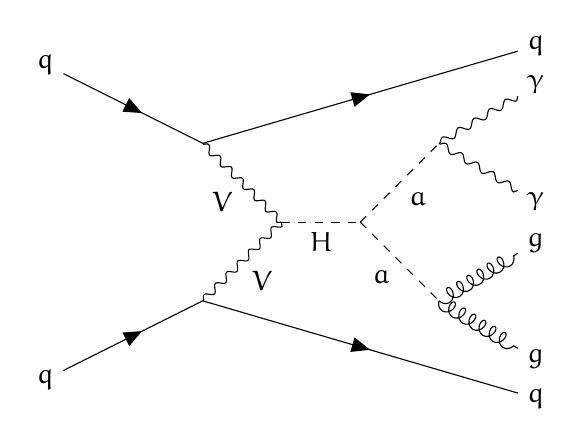
\begin{tikzpicture}
      \begin{feynman}
        \vertex (q1init) {\(q\)};
        \vertex [below =4. of q1init] (q2init) {\(q\)};
        \vertex [below right=1. and 2. of q1init] (qqV);
        \vertex [above right=1. and 2. of q2init] (qqV2);
        \vertex [above right=1. and 4. of  qqV] (q1final) {\(q\)};
        \vertex [below right=1. and 4. of qqV2] (q2final) {\(q\)};
        \vertex [below right=1. and 1. of qqV] (VVH);
        \vertex [right=1. of VVH] (H);
        \vertex [above right=1. and 1. of H] (ayy);
        \vertex [below right=1. and 1. of H] (agg);
        \vertex [above right=0.5 and 1. of ayy] (y1) {\(\gamma\)};
        \vertex [below right=0.5 and 1. of ayy] (y2) {\(\gamma\)};
        \vertex [above right=0.5 and 1. of agg] (g1) {\(g\)};
        \vertex [below right=0.5 and 1. of agg] (g2) {\(g\)};
        \diagram* {
          (q1init) -- [fermion] (qqV) -- [fermion] (q1final),
          (q2init) -- [fermion] (qqV2) -- [fermion] (q2final),
          (qqV) -- [boson, edge label'=\(V\)] (VVH),
          (qqV2) -- [boson, edge label'=\(V\)] (VVH),
          (VVH) -- [scalar, edge label'=\(H\)] (H),
          (H) -- [scalar, edge label'=\(a\)] (ayy),
          (H) -- [scalar, edge label'=\(a\)] (agg),
          (ayy) -- [photon] (y1),
          (ayy) -- [photon] (y2),
          (agg) -- [gluon] (g1),
          (agg) -- [gluon] (g2),
        };
      \end{feynman}
    \end{tikzpicture}
    \label{fig:VBFH_feynman}
  }
  \caption{
    (a) Projected branching ratio for $H\rightarrow \gamma\gamma gg$ in order to make a discovery of new physics at a significance level of $5\sigma$, as a function of integrated luminosity, when searching in the gluon fusion (GGH), vector boson fusion (VBF), and associated production (VH) production modes.
    The projection for GGH and VBF assumes a $20\%$ systematic uncertainty due to jet reconstruction effects, while the projection for VH uses the estimation from Ref.~\cite{hep-ph/0703247}, assuming the significance is statistics-dominated.
    With less than $\sim 20 \ifb$, the gluon fusion mode is most sensitive, but with more statistics this production mode quickly becomes dominated by systematic uncertainties and is unable to provide better limits.
    Up to $\sim 300 \ifb$, the VBF mode is most sensitive; in Run 2 the LHC has gathered 140$\ifb$.
    With more than $\sim 300 \ifb$, the VH mode likely provides the best sensitivity.
    (b) Tree-level diagram of production and decay of Higgs boson being searched for in this analysis.
    }
\end{figure}

This search presents many interesting areas of original research in order to improve the sensitivity of the analysis.
The fully reconstructed final state contains four jets;
the main challenges present in this analysis involve reconstructing and identifying these jets.

When reconstructing the energy of the originating parton of a jet, both the effects of the energy response of the calorimeter and the effect of other proton-proton interactions in the event (pile-up) must be taken into account.
Chapter~\ref{ch:NI} presents work on studying in a rigorous framework the mathematical process of reversing the effects of the calorimeter response in order to access the originating parton energy (\cite{Cukierman:2016dkb});
and Chapter~\ref{ch:Calib} presents work on using machine learning to further improve this process.
Appendix~\ref{ch:Voronoi} presents work on novel jet reconstruction algorithms which aim to reduce the effect of pileup on the jet reconstructed energy~\cite{ATLAS-CONF-2017-065}.
These efforts serve to develop new techniques for reconstructing the energies of the jets that appear in the final state of this analysis, and therefore improve the ultimate sensitivity of this search.
These techniques can also be effective in the higher pileup conditions expected at the LHC in Run 3 and beyond, and are intended to be broadly applicable to other analyses than the one being studied here. 

\section{Data and simulation}

The search presented in this chapter is based on the 36.7~\ifb{} dataset of proton--proton collisions
recorded by the ATLAS experiment at the LHC at $\sqrt{s}=13$ \TeV{} during 2015 and 2016.
The ATLAS detector~\cite{PERF-2007-01} comprises an inner detector in a 2 T axial magnetic field, 
for tracking charged particles and a precise localisation of the interaction vertex, 
a finely segmented calorimeter, a muon spectrometer and a two-level trigger~\cite{TRIG-2016-01} that
accepts about 1 kHz rate for data storage.

Monte Carlo (MC) event generators were used to simulate the $H\to aa \to \gamma\gamma gg$ signal.
Signal samples for the ggF and VBF processes were generated at next-to-leading order using 
\POWHEGBOX{}~\cite{Nason:2004rx,Frixione:2007vw,Alioli:2010xd} interfaced with \PYTHIA{}~\cite{Sjostrand:2014zea} for parton showering and hadronisation using the AZNLO set of tuned parameters set~\cite{STDM-2012-23} and the CT10 parton distribution function (PDF) set~\cite{Lai:2010vv}.
Samples were generated in the $m_a$ range\footnote{The diphoton triggers considered for this
search do not have acceptance for the lower mass range ($m_a<20~\GeV{}$), where the two photons are collimated.} 
$20~\GeV{} < m_a < 60~\GeV{}$, assuming the $a$ boson to be a (pseudo)scalar.
All MC event samples were processed through a detailed simulation~\cite{SOFT-2010-01} of the ATLAS detector
based on \geantFour{}~\cite{Agostinelli:2002hh}, and contributions from additional $pp$ interactions (pile-up), simulated using
\PYTHIA{} and the MSTW2008LO PDF set~\cite{Martin:2009iq}, were overlaid onto the hard-scatter events.

\section{Selection criteria}

Events are selected by two diphoton triggers.
One trigger path requires the presence in the electromagnetic (EM) calorimeter of two clusters of energy
deposits with transverse energy\footnote{ATLAS uses a right-handed coordinate system with its origin 
  at the nominal interaction point (IP) in the centre of the detector and the $z$-axis along the beam pipe. The $x$-axis points from the IP to the centre of the LHC ring, 
  and the $y$-axis points upward. Cylindrical coordinates $(r,\phi)$ are used in the transverse plane, $\phi$ being the azimuthal angle around the $z$-axis. 
  The pseudorapidity is defined in terms of the polar angle $\theta$ as $\eta=-\ln\tan(\theta/2)$.}
above 35 \GeV{} and 25 \GeV{} for the leading (highest transverse energy) and sub-leading
(second-highest transverse energy) clusters, respectively. In the high-level trigger the shape of the energy
deposit in both clusters is required to be loosely consistent with that expected from an EM shower initiated by a photon.
The other trigger path requires the presence of two clusters with transverse energy above 22 \GeV{}.
In order to suppress the additional rate due to the lower transverse energy threshold, the shape requirements for the energy deposits are
more stringent.

The photon candidates are reconstructed from the clusters of energy deposits in the EM calorimeter within the range $|\eta|<2.37$.
The energies of the clusters are calibrated to account for energy losses upstream of the calorimeter 
and for energy leakage outside the cluster, as well as other effects due to the detector geometry and response.
The calibration is refined by applying $\eta$-dependent correction factors of the order of $\pm1$\%, derived from $Z\to ee$ events~\cite{PERF-2013-05}.
As in the trigger selection, photon candidates are required to satisfy a set of identification criteria based on the shape of the EM cluster~\cite{PERF-2013-04}.
Two working points are defined: a \textit{Loose} working point, used for the preselection and the data-driven background estimation, and a 
\textit{Tight} working point, with requirements that further reduce the misidentification of neutral hadrons decaying to two photons.
In order to reject the hadronic jet background, photon candidates are required to be isolated from any other activity in the calorimeter.
The calorimeter isolation is defined as the sum of the transverse energy in the
calorimeter within a cone of \mbox{$\Delta R = \sqrt{(\Delta\eta)^2+(\Delta\phi)^2}=0.4$} centred around the photon candidate,
The transverse energy of the photon candidate is subtracted from the calorimeter isolation.
Contributions to the calorimeter isolation from the underlying event and pile-up are subtracted using the method proposed in Ref.~\cite{jetareas}.
Candidates with a calorimeter isolation larger than 2.2\% of the photon's transverse energy are rejected.

Jets are reconstructed from topological clusters~\cite{PERF-2014-07} using the anti-$k_t$
algorithm~\cite{Cacciari:2008gp} implemented in the FastJet package~\cite{Cacciari:2011ma} with a radius parameter of $R=0.4$. 
Jets are calibrated using an energy- and $\eta$-dependent
calibration scheme, and are required to have a transverse momentum (\pt{}) greater than $20~\GeV{}$ and $|\eta|<2.5$ or $\pt>30~\GeV{}$ and $|\eta|<4.4$.
A track- and topology-based veto~\cite{PERF-2014-03,PERF-2016-06} is used to suppress jets originating from pile-up interactions.
Jets must have an angular separation of $\Delta R>0.4$ from any \textit{Loose} photon candidate in the event.

\begin{figure}[t]
  \centering 
  \subfloat[]{\includegraphics[width=0.45\textwidth]{figures/{vbf_mjj_shape_log_VBF8_combined_8.7.17}.pdf}\label{fig:dista}}
  \subfloat[]{\includegraphics[width=0.45\textwidth]{figures/{vbf_jet1pt_postselection_shape_log_VBF8_combined_8.7.17}.pdf}\label{fig:distb}}\\
  \subfloat[]{\includegraphics[width=0.45\textwidth]{figures/{hmass_amassdiff_shape_VBF8_combined_8.7.17}.pdf}\label{fig:distd}}
  \subfloat[]{\includegraphics[width=0.45\textwidth]{figures/{amassdiff_shape_VBF8_combined_8.7.17}.pdf}\label{fig:distc}}
  \caption{
    Distributions of kinematic observables before the requirements on \smash{$m_{jj}^\text{VBF}$}, leading VBF jet \pt{}, \smash{$m_{\gamma\gamma jj}$}
    and $|m_{jj}-m_{\gamma\gamma}|$ for:
    (a) $m_{jj}^\text{VBF}$; (b) leading VBF jet \pt{};
    (c) $m_{\gamma\gamma jj}$ (with the additional requirement $|m_{jj}-m_{\gamma\gamma}|< 12~\GeV{}$ 
    that defines the signal-enriched region); and (d) $|m_{jj}-m_{\gamma\gamma}|$.
    The quantities are shown separately for simulated signal events (with $m_a=30$ \GeV{}) produced in the VBF mode 
    and compared with those produced in the ggF mode and the observed data.
    }
  \label{fig:dist}
\end{figure}

Events are required to have at least two photon candidates. 
The transverse energy requirements depend on the trigger path through which the event was recorded.
For events passing the trigger with higher transverse energy thresholds, the leading photon is required to have $E_\text{T}>40$ \GeV{}, 
and the sub-leading photon is required to have $E_\text{T}>30$ \GeV{}. For events passing the trigger with lower thresholds, 
both the leading and sub-leading photons are required to have $E_\text{T}>27$ \GeV{}. 
For events passing both triggers, the latter selection is applied.
The invariant mass of the two leading photon candidates is denoted by $m_{\gamma\gamma}$.

In the VBF production mode, the Higgs boson is produced in association with two additional light-quark jets
with a large opening angle and a large invariant mass.
Selected events are therefore required to have at least four jets and 
the pair of jets with the highest invariant mass ($m_{jj}^\text{VBF}$) are referred to as \textit{VBF jets}.
In VBF signal events, these jets correspond to the light quarks emitting the vector bosons 55\% of the time, 
as estimated in simulation.
The VBF Higgs boson signal is further enhanced,
relative to the dominant $\gamma\gamma$+multi-jet background,
by requiring $m_{jj}^\text{VBF}$ to be greater than 500 \GeV{} and 
the \pt{} of the leading VBF jet to be greater than 60 \GeV{}.
The discrimination power of these observables can be seen in the difference in shape between the VBF signal and the 
data, shown in Figures~\ref{fig:dista} and \ref{fig:distb}.
The two remaining highest-\pt{} jets are referred to as \textit{signal jets}, with invariant mass $m_{jj}$.
The two photon candidates and the two signal jets form the Higgs boson candidate with invariant mass $m_{\gamma\gamma jj}$, 
which is required to be in the range $100 < m_{\gamma\gamma jj} < 150~\GeV{}$. 
Figure~\ref{fig:distd} shows that most of the selected signal events lie within this range, 
while the data have a broad distribution extending to higher values.

In order to take advantage of the $m_{\gamma\gamma}$ resolution of about 1.3 \GeV{} to suppress the background with $m_{\gamma\gamma}$ far from the
range of interest, five overlapping $m_{\gamma\gamma}$ regimes are defined as summarised in Table~\ref{tab:amassdiffcut}.
The boundaries of the $m_{\gamma\gamma}$ regimes are chosen so that for any value of $m_a$ 
considered in the scope of this search there is at least one regime where there is no significant signal acceptance loss
due to the $m_{\gamma\gamma}$ requirement.
For each $m_{\gamma\gamma}$ regime, the set of $m_a$ values for which this requirement causes no significant signal acceptance loss is also indicated.

\section{Background estimation}

The $\gamma\gamma$+multi-jet background consists of multi-jet events with two reconstructed photon candidates, 
originating from isolated EM radiation or from jets.
A data-driven estimation based on two-dimensional sidebands is used to predict the background yields.
The method consists of using two uncorrelated observables
to define four regions labelled A, B, C and D.

The first axis of the A/B/C/D plane separates events in regions C and D with both photons passing the \textit{Tight} requirement 
from events in regions A and B with at most one photon 
passing the \textit{Tight} requirement and at least one passing the \textit{Loose} but not the \textit{Tight} requirement. 
These regions are referred to respectively as \textit{Tight--Tight} (C and D) and \textit{Tight--Loose} (A and B). 

The second axis separates events in regions B and D, satisfying $|m_{jj}-m_{\gamma\gamma}|< x_\text{R}$, 
from events in regions A and C, satisfying $|m_{jj}-m_{\gamma\gamma}|>x_\text{R}$. 
The value $x_\text{R}$ depends on the $m_{\gamma\gamma}$ regime R to account for the degradation in resolution at higher mass.
For $H\to aa \to \gamma\gamma gg$ signal events, where the $a$ boson candidates have similar masses, the difference $|m_{jj}-m_{\gamma\gamma}|$ tends to be smaller, 
as shown in Figure~\ref{fig:distc}.
The signal events that lie outside of the range $|m_{jj}-m_{\gamma\gamma}|< x_\text{R}$ are due to poor $m_{jj}$ resolution or to incorrect assignment of the jets corresponding 
to the gluons originating from the $a$ boson decay.
Specific $x_\text{R}$ values are given in Table~\ref{tab:amassdiffcut}.
In each $m_{\gamma\gamma}$ regime, the boundary for $|m_{jj}-m_{\gamma\gamma}|$ is 0.4 times the central $m_{\gamma\gamma}$ value.
An exception is made for the lowest $m_{\gamma\gamma}$ regime, where $x_\text{R}$ is larger in order to increase the signal efficiency.

\begin{table}[t]
  \begin{center}
    \caption{
      Definition of each $m_{\gamma\gamma}$ regime, the range of $m_a$ values considered in the scope of this search with no significant signal loss acceptance due to the $m_{\gamma\gamma}$ requirement, and the corresponding boundary $x_\text{R}$ for $|m_{jj}-m_{\gamma\gamma}|$.  
    }
  \label{tab:amassdiffcut}
    {\footnotesize
  \begin{tabular}{ c c c c }
    \toprule
    $m_{\gamma\gamma}$ regime & Definition & Range of $m_a$ values & $x_\text{R}$ [\GeV{}] \\
    \midrule
    1 & $17.5$ \GeV{} $< m_{\gamma\gamma}< 27.5$ \GeV{} & $20$ \GeV{} $\le m_a \le 25$ \GeV{} & 12 \\
      2 & $22.5$ \GeV{} $< m_{\gamma\gamma}< 37.5$ \GeV{} & $25$ \GeV{} $\le m_a \le 35$ \GeV{} & 12 \\
      3 & $32.5$ \GeV{} $< m_{\gamma\gamma}< 47.5$ \GeV{} & $35$ \GeV{} $\le m_a \le 45$ \GeV{} & 16 \\
      4 & $42.5$ \GeV{} $< m_{\gamma\gamma}< 57.5$ \GeV{} & $45$ \GeV{} $\le m_a \le 55$ \GeV{} & 20 \\
      5 & $52.5$ \GeV{} $< m_{\gamma\gamma}< 65.0$ \GeV{} & $55$ \GeV{} $\le m_a \le 60$ \GeV{} & 24 \\
    \bottomrule
  \end{tabular}
    }
  \end{center}
\end{table}

Region D is expected to contain the highest contribution of signal. 
In this region, 60\% of the signal events are produced in the VBF mode and the remaining 40\% in the ggF mode.
Assuming no correlation in the background events between the two observables used to define the A/B/C/D regions,
the number of background events in the signal region D ($N^\text{bkg}_\text{D}$) is related to the number
of background events in the control regions A, B and C, denoted by $N^\text{bkg}_\text{A}$, $N^\text{bkg}_\text{B}$
and $N^\text{bkg}_\text{C}$, respectively, by the formula
\begin{align}
N^\text{bkg}_\text{D} = \frac{N^\text{bkg}_\text{B}N^\text{bkg}_\text{C}}{N^\text{bkg}_\text{A}}.
\label{eqn:closure}
\end{align}
In the following, the difference between the prediction $N^\text{bkg}_\text{D}$ and the actual background yield in region D 
is referred to as \textit{non-closure}.
The non-closure results from residual correlations between the two observables used to define the A/B/C/D regions,
and the uncertainty accounting for this effect is referred to as \textit{closure uncertainty}.
In order to quantify the non-closure, the data-driven estimation as described above is performed 
with the exception that the requirement on $m_{\gamma\gamma jj}$ is inverted.
For each $m_{\gamma\gamma}$ regime,
the closure uncertainty is defined to be 
the central value of the non-closure if it is found to be significant ($>1\sigma$) in comparison with its statistical uncertainty; 
otherwise, the statistical uncertainty of its estimate is used.

\section{Results}

The efficiency of the event selection for the $pp\to H\to aa \to \gamma\gamma gg$ signal in each of the A/B/C/D regions is shown in Table~\ref{tab:ABCD},
assuming the SM cross-section and kinematics for the different production modes as described in Ref.~\cite{deFlorian:2016spz}.
The observed number of events in each of the A/B/C/D regions for each $m_{\gamma\gamma}$ regime is shown in Table~\ref{tab:ABCD_data}
along with the predicted background in the signal region D, taking into account the closure uncertainty. 
Due to the low event counts in each of the A/B/C/D regions,
the median expected background yield in region D estimated from pseudo-data experiments involving asymmetric Poisson uncertainties 
in the different regions slightly differs from the direct estimation from Eq.~(\ref{eqn:closure}).
No large excess is observed in region D when comparing the data yield to the background predicted from the A/B/C regions
assuming that the signal is absent in these regions.
However, given that a signal contamination is possible, a more refined procedure
taking into account signal contributions in all regions
is employed to set limits on the production rate of $H\to aa \to \gamma\gamma gg$.

\begin{table}[t]
  \begin{center}
    \caption{Efficiency of event selection on the $pp\to H\to aa \to \gamma\gamma gg$ signal, 
      assuming the SM Higgs boson production cross-section and kinematics,
      in each of the A/B/C/D regions, for different $m_a$ mass hypotheses.
      For each $m_a$ value, all $m_{\gamma\gamma}$ regimes in which there is no significant signal acceptance loss due to the $m_{\gamma\gamma}$ requirement are shown.
    }
    \label{tab:ABCD}
    \footnotesize
    \bgroup
    \def\arraystretch{1.5}
    \begin{tabular}{
        c
        c
        r@{}l
        r@{}l
        r@{}l
        r@{}l
      }
      \hline
      {$m_a$ [\GeV{}]} & {$m_{\gamma\gamma}$ regime} & \multicolumn{8}{c}{Efficiency $(\times 10^{-5})$}  \\
      & & \multicolumn{2}{c}{A} & \multicolumn{2}{c}{B} & \multicolumn{2}{c}{C} & \multicolumn{2}{c}{D}  \\
      \hline
      20 & 1 & 0.50&$^{+0.16}_{-0.14}$ & 1.2&$\pm0.4$ & 3.9&$\pm1.1$           & 6.2&$\pm1.8$           \\
      25 & 1 & 0.67&$^{+0.27}_{-0.33}$ & 2.6&$^{+0.5}_{-0.6}$ & 5.8&$\pm1.4$           & 15&$\pm4$           \\ 
      25 & 2 & 0.67&$^{+0.27}_{-0.33}$ & 2.6&$^{+0.5}_{-0.6}$ & 5.8&$\pm1.4$           & 15&$\pm4$           \\ 
      30 & 2 & 1.22&$\pm0.34$           & 3.3&$\pm0.9$          & 7.6&$^{+1.4}_{-1.6}$   & 25&$^{+5}_{-6}$   \\
      35 & 2 & 1.8&$\pm1.1$            & 2.7&$\pm1.2$           & 9.3&$\pm2.6$           & 27&$\pm6$           \\ 
      35 & 3 & 0.53&$^{+1.20}_{-0.24}$  & 4.1&$\pm1.2$           & 6.1&$^{+1.2}_{-1.6}$   & 31&$\pm7$           \\
      40 & 3 &  1.2&$\pm0.4$           & 3.3&$\pm1.0$           & 7.9&$^{+1.7}_{-2.4}$   & 26&$\pm6$           \\
      45 & 3 & 2.5&$\pm1.0$           & 4.1&$\pm1.3$           & 7.7&$^{+1.7}_{-2.0}$   & 19&$\pm5$           \\ 
      45 & 4 & 2.2&$\pm0.9$  & 4.4&$\pm1.4$           & 5.9&$^{+1.5}_{-2.2}$   & 22&$\pm5$           \\ 
      50 & 4 &  0.93&$\pm0.30$           & 4.4&$\pm1.2$           & 5.0&$^{+1.3}_{-1.0}$   & 24&$\pm5$   \\
      55 & 4 & 0.37&$\pm0.11$          & 3.3&$\pm0.9$          & 5.4&$^{+1.3}_{-1.4}$   & 21&$\pm5$           \\ 
      55 & 5 & 0.23&$\pm0.16$          & 3.6&$\pm1.0$          & 3.4&$\pm0.8$          & 24&$\pm6$           \\ 
      60 & 5 &  0.77&$^{+0.32}_{-0.30}$  & 3.9&$\pm1.0$           & 4.9&$\pm1.4$           & 23&$\pm6$           \\
      \hline
    \end{tabular}
    \egroup
  \end{center}
\end{table}

\begin{table}[t]
  \begin{center}
    \caption{Number of events observed in each of the A/B/C/D regions, 
      the relative size of the closure uncertainty considered for each $m_{\gamma\gamma}$ regime, 
      and the prediction for the number of background events in region D based on the control region yields.
      The median predicted background yield and its $\pm1\sigma$ uncertainty in region D is also shown.
      The uncertainties in the prediction account for both the Poisson fluctuations of the number of events in the control regions 
      and the closure uncertainty.
    }
    \label{tab:ABCD_data}
          {\footnotesize
            \bgroup
            \def\arraystretch{1.3}
	    \begin{tabular}{
                ccccccr@{}l
              }
	      \hline
              $m_{\gamma\gamma}$ regime &   A &   B &   C &   D  & Relative closure uncert. & \multicolumn{2}{c}{Predicted background yield}\\
	      \hline
              1 &  15 &   4 &  28 &   4 &  0.50 & \hspace{1.4cm}6&$^{+7}_{-4}$   \\
              2 &  22 &   6 &  34 &  15 &  0.32 & 8&$^{+7}_{-4}$   \\
              3 &  12 &  16 &  29 &  26 &  0.20 & 37&$^{+23}_{-14}$ \\
              4 &   8 &  12 &  19 &  38 &  0.21 & 27&$^{+22}_{-12}$ \\
              5 &   6 &  20 &  20 &  36 &  0.20 & 66&$^{+56}_{-28}$ \\
	      \hline
	    \end{tabular}
            \egroup
          }
  \end{center}
\end{table}

A likelihood function, describing both the expected background and signal, is fit to all four A/B/C/D regions simultaneously.
The free parameters of the likelihood are the numbers of signal and background events in region D, 
$\mu_\text{S}$ and $\mu_\text{bkg}$ respectively, the ratio of background events expected in region B to that in region D, $\tau_\text{B}$, 
and the analogous ratio for region C, $\tau_\text{C}$.
The assumption of no correlation in the total background, Eq.~(\ref{eqn:closure}), 
allows the background to be parameterised in terms of only three parameters.
The closure uncertainty, which accounts for the uncertainty due to assuming non-correlation, is included in the likelihood function by applying a Gaussian prior
to the expected number of background events in region A, $\tau_\text{B}\tau_\text{C}\mu_\text{bkg}$.
The Gaussian width is determined by the size of the closure uncertainty summarized in Table~\ref{tab:ABCD_data}.
The parameter $\mu_\text{S}$ can be expressed as the product of the total integrated luminosity, the signal cross-section 
$\sigma_H\times B(H\to aa\to \gamma\gamma gg)$, and the signal selection efficiency estimated in MC simulation
and quoted in Table~\ref{tab:ABCD}.
The signal contamination in the control regions A, B, and C is estimated from MC simulation 
and is varied coherently with $\mu_\text{S}$ in the likelihood fit.

The low number of observed events is the dominant source of uncertainty for this search.
The second largest uncertainty is due to the closure uncertainty, also statistical in nature.
Other sources of systematic uncertainty only affect the overall signal normalisation and the amount of signal contamination
in control regions A, B and C.
Dominant sources of experimental systematic uncertainty arise from the calibration and resolution of the energy of the 
jets~\cite{PERF-2016-04,PERF-2011-04}. 
Uncertainties associated with the photon energy calibration and resolution~\cite{PERF-2013-05}, as well as the photon identification and isolation
efficiencies~\cite{PERF-2013-04}, are found to be negligible. Uncertainties associated 
with the estimation of the integrated luminosity and the simulation of pile-up interactions (\textit{Lumi and Pile-up})
are found to be negligible. 
The systematic uncertainty associated with the modelling of the kinematics in signal 
events (\textit{Modelling}) is evaluated by varying the choice of scales used in the generator program and
assuming the SM Higgs boson production~\cite{Heinemeyer:2013tqa}.
It is found to be similar in size to the experimental systematic uncertainty.

Nuisance parameters corresponding to each source of uncertainty are included in the profile likelihood as Gaussian constraints.
Their effects on the estimated number of signal events $\mu_\text{S}$ are studied using Asimov~\cite{Cowan:2010js} pseudo-datasets generated
for an expected signal corresponding to the 95\% CL upper limit obtained in this search and using the values of the background 
parameters maximising the likelihood in a fit to data which assumes no signal.
Table~\ref{tab:systs} summarises the impact of each source of uncertainty varied by $\pm1\sigma$ on the maximum-likelihood estimate for $\mu_\text{S}$ in each 
of the $m_{\gamma\gamma}$ regimes for an illustrative $m_a$ hypothesis. The statistical uncertainty is the largest one for all regimes.
\begin{table}[t]
  \begin{center}
    \caption{
      Maximum fractional impact on the fitted $\mu_\text{S}$ from sources of systematic uncertainty estimated using Asimov datasets.
      The signal injected in the Asimov datasets corresponds to the observed upper limit quoted in Table~\ref{tab:limits}.
    }
    \label{tab:systs}
          {\footnotesize
	  \begin{tabular}{cccccc}
	  \hline
          &\multicolumn{5}{c}{$m_{\gamma\gamma}$ regime} \\
          Source of Uncert.   &    1  &   2  &   3  &   4  &   5  \\
            &   $m_a=20~\GeV{}$ &  $m_a=30~\GeV{}$ &  $m_a=40~\GeV{}$ &  $m_a=50~\GeV{}$ &  $m_a=60~\GeV{}$ \\
          \hline
	  Statistical          &     0.73 &     0.51 &     0.89 &     1.13 &     0.92 \\
	  Closure              &     0.44 &     0.27 &     0.39 &     0.64 &     0.89 \\
	  \hline
	  Modelling            &     0.35 &     0.34 &     0.46 &     0.42 &     0.65 \\
	  Jet                  &     0.58 &     0.38 &     0.25 &     0.90 &     0.71 \\
	  Photon               &     0.06 &     0.05 &     0.10 &     0.12 &     0.13 \\
	  Lumi and Pile-up     &     0.06 &     0.04 &     0.27 &     0.14 &     0.32 \\
	  \hline
	  \end{tabular}
          }
  \end{center}
\end{table}
The best-fit values of the parameters of the likelihood function are given in Table~\ref{tab:MLE}.
The probability that the data are compatible with the background-only hypothesis is computed for each $m_{\gamma\gamma}$ regime and no significant 
excess is observed. The smallest local $p$-value, obtained for the $m_{\gamma\gamma}$ regime 2 ($m_a\approx30~\GeV{}$), is of the order of 4\%.
\begin{table}[t]
  \begin{center}
    \caption{Maximum-likelihood fit values for each of the free parameters of the likelihood function 
      in each $m_{\gamma\gamma}$ regime for a relevant signal $m_a$ hypothesis.
      The estimated uncertainties in the fit parameters assume
      that the likelihood function is parabolic around the minimum of the fit.
    }
    \label{tab:MLE}
          {\footnotesize
	    \begin{tabular}{
                cc
                r@{}lr@{}l
                r@{}lr@{}l
              }
	      \hline
              $m_{\gamma\gamma}$ regime & $m_a$ [\GeV{}] &   \multicolumn{2}{c}{$\mu_\text{S}$} &   \multicolumn{2}{c}{$\mu_\text{bkg}$}  &   \multicolumn{2}{c}{$\tau_\text{B}$} & \multicolumn{2}{c}{$\tau_\text{C}$} \\
	      \hline
              1 & 20 &  -7&$\pm$18    & 11&$\pm$17   & 0.5 &$\pm$0.4 &  2.9&$\pm$3.1   \\
              2 & 30 &  8&$\pm$8      & 7&$\pm$6     & 0.68 &$\pm$0.32 & 4.3&$\pm$3.1   \\
              3 & 40 &  -30&$\pm$80   & 60&$\pm$70   & 0.35 &$\pm$0.19 & 0.67&$\pm$0.33 \\
              4 & 50 &  22&$\pm$28    & 16&$\pm$23   & 0.5 &$\pm$0.4 & 0.9&$\pm$1.0   \\
              5 & 60 &  -290&$\pm$260 & 340&$\pm$340 & 0.21&$\pm$0.05 & 0.24&$\pm$0.05 \\
	      \hline
	    \end{tabular}
          }
  \end{center}
\end{table}
Since no significant excess is observed, an upper limit is derived at 95\% CL.            
The expected and observed exclusion limits on $\mu_\text{S}$ are given in Table~\ref{tab:limits}.
This is related to the limit on the $pp\to H\to aa \to \gamma\gamma gg$ cross-section by appropriately normalising to the measured total integrated luminosity 
and selection efficiencies relative to the inclusive signal production obtained from the ggF and VBF MC samples (Table~\ref{tab:ABCD}).
The limit is also expressed relative to the SM cross-section for the Higgs boson, shown in Figure~\ref{fig:brazil_ma}.
Within a $m_{\gamma\gamma}$ analysis regime, limits are interpolated linearly in between simulated $m_a$ values.
Finally, for each mass point, the $m_{\gamma\gamma}$ regime that yields the best expected limit is used to provide the observed exclusion limit.
The limit is calculated using a frequentist $\text{CL}_\text{s}$ calculation~\cite{Read:2002hq}. 

\begin{table}[t]
  \begin{center}
    \caption{Observed (expected) upper limits at the 95\% CL, for each of the $m_a$ values considered in the search.
      In each case, the $m_{\gamma\gamma}$ regime used to calculate the limits is also indicated.
      The uncertainties include both the statistical and systematic sources of uncertainty in the fit.}
    \label{tab:limits}
          {\footnotesize
            \bgroup
            \def\arraystretch{1.5}
            \begin{tabular}{ccr@{}lr@{}lr@{}l}
	    \hline
            $m_{\gamma\gamma}$ regime & $m_a$ [\GeV{}] & \multicolumn{2}{c}{$\mu_\text{S}$}   & \multicolumn{2}{c}{$\sigma_H\times B(H\to aa \to \gamma\gamma gg)$ [pb]}  & \multicolumn{2}{c}{$\frac{\sigma_H}{\sigma_\text{SM}}\times B(H\to aa \to \gamma\gamma gg)$} \\
	    \hline
            1 & 20 & $10.8\Big(10.4$&$^{+4.6}_{-3.1}\Big)$   & \hspace{1.1cm}$4.8\Big(4.6$&$^{+2.1}_{-1.4}\Big)$  & \hspace{0.505cm}$0.086\Big(0.082$&$^{+0.037}_{-0.025}\Big)$ \\
            1 & 25 & $10.4\Big(10.9$&$^{+3.8}_{-2.5}\Big)$   & $1.9\Big(2.0$&$^{+0.7}_{-0.5}\Big)$  & $0.034\Big(0.036$&$^{+0.013}_{-0.008}\Big)$ \\
            2 & 25 & $28\Big(25$&$^{+8}_{-6}\Big)$   & $5.1\Big(4.7$&$^{+1.4}_{-1.1}\Big)$  & $0.092\Big(0.084$&$^{+0.026}_{-0.019}\Big)$ \\
            2 & 30 & $29\Big(24$&$^{+11}_{-6}\Big)$  & $3.1\Big(2.6$&$^{+1.1}_{-0.7}\Big)$ & $0.056\Big(0.046$&$^{+0.021}_{-0.012}\Big)$ \\
            2 & 35 & $27\Big(22$&$^{+9}_{-6}\Big)$   & $2.7\Big(2.2$&$^{+0.9}_{-0.6}\Big)$ & $0.049\Big(0.040$&$^{+0.016}_{-0.011}\Big)$  \\
            3 & 35 & $30\Big(36$&$^{+18}_{-9}\Big)$  & $2.7\Big(3.2$&$^{+1.6}_{-0.8}\Big)$ & $0.048\Big(0.057$&$^{+0.028}_{-0.014}\Big)$  \\
            3 & 40 & $31\Big(39$&$^{+19}_{-12}\Big)$ & $3.2\Big(4.0$&$^{+2.0}_{-1.2}\Big)$  & $0.058\Big(0.073$&$^{+0.035}_{-0.022}\Big)$ \\
            3 & 45 & $45\Big(53$&$^{+15}_{-20}\Big)$ & $6.3\Big(7.5$&$^{+2.1}_{-2.8}\Big)$   & $0.113\Big(0.134$&$^{+0.038}_{-0.050}\Big)$     \\
            4 & 45 & $74\Big(68$&$^{+16}_{-15}\Big)$ & $9.2\Big(8.4$&$^{+2.0}_{-1.9}\Big)$  & $0.166\Big(0.152$&$^{+0.036}_{-0.034}\Big)$ \\
            4 & 50 & $79\Big(77$&$^{+17}_{-16}\Big)$ & $9.0\Big(8.8$&$^{+2.0}_{-1.8}\Big)$  & $0.162\Big(0.159$&$^{+0.036}_{-0.032}\Big)$   \\
            4 & 55 & $73\Big(69$&$^{+11}_{-10}\Big)$  & $9.7\Big(9.1$&$^{+1.5}_{-1.2}\Big)$   & $0.173\Big(0.163$&$^{+0.026}_{-0.022}\Big)$    \\
            5 & 55 & $48\Big(59$&$^{+41}_{-19}\Big)$ & $5.5\Big(6.8$&$^{+4.7}_{-2.1}\Big)$  & $0.10\Big(0.12$&$^{+0.08}_{-0.04}\Big)$ \\
            5 & 60 & $67\Big(81$&$^{+24}_{-31}\Big)$ & $8.0\Big(9.5$&$^{+2.8}_{-3.6}\Big)$  & $0.14\Big(0.17$&$^{+0.05}_{-0.07}\Big)$   \\
	    \hline
	    \end{tabular}
            \egroup
          }
  \end{center}
\end{table}

\begin{figure}[t]
  \centering 
  {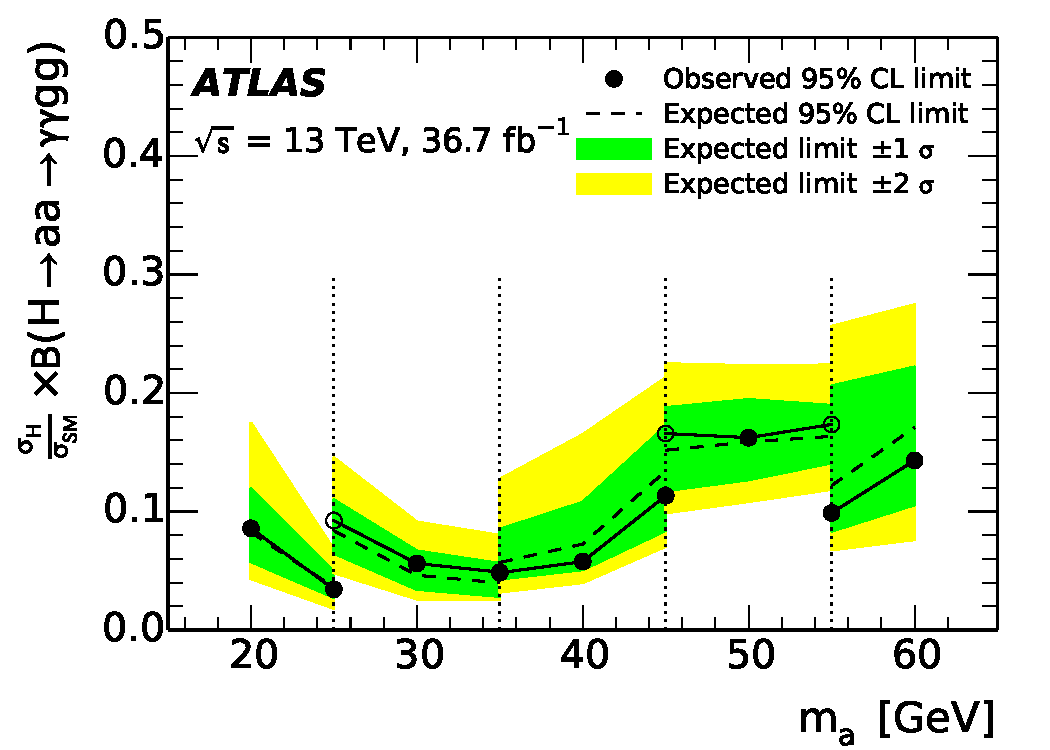
\includegraphics[width=0.9\textwidth]{figures/ABCD_twosigma_brazil_Freq_systs_obs_HF_ma_2_16_18.pdf}}
  \caption{The observed (solid line) and expected (dashed line) 95\% CL exclusion upper limit on 
    the \mbox{$pp\to H\to aa \to \gamma\gamma gg$} cross-section times branching ratio as a function of $m_a$,
    normalised to the SM inclusive $pp\to H$ cross-section~\cite{deFlorian:2016spz}.
  The vertical lines indicate the boundaries between the different $m_{\gamma\gamma}$ analysis regimes.
  At the boundaries, the $m_{\gamma\gamma}$ regime that yields the best expected limit is used to provide the observed exclusion limit (filled circles); the observed limit provided by the regime that yields the worse limit is also indicated (empty circles).
}
  \label{fig:brazil_ma}
\end{figure}

\section{Conclusions}

In summary, a search for exotic decays of the Higgs boson into a pair of new (pseudo)scalar particles,
$H\to aa$, in final states with two photons 
and two jets is conducted using 36.7~\ifb{} of $pp$ collisions at $\sqrt{s}=13$ \TeV{} recorded 
with the ATLAS detector at the LHC. The search for $H\to aa \to \gamma\gamma gg$ is performed
in the mass range $20 < m_a < 60~\GeV{}$ and with additional jet requirements 
to enhance VBF-produced signal while suppressing the $\gamma\gamma$+jets background.
No significant excess of data is observed relative to the SM predictions. An upper limit
is set for the product of the production cross-section for $pp\to H$ and the branching
ratio for the decay $H\to aa\to\gamma\gamma gg$. The upper limit ranges from 3.1 pb to 9.0 pb depending
on $m_a$, and is mostly driven by the statistical uncertainties.
These results complement the previous upper limit on $H\to aa\to\gamma\gamma\gamma\gamma$ and
further constrains the BSM parameter space for exotic decays of the Higgs boson.

%Another challenge present in this analysis is identifying and labeling the jets in the event as coming from the final state gluons, the quarks from the VBF production, or from pileup or underlying event.
%Tackling this challenge will involve utilizing newly developed techniques in quark-gluon tagging and pileup mitigation, including in the particularly difficult forward region of the calorimeter.
%Particularly challenging is the low-$m_a$ regime of the parameter space;
%in this regime, the gluons produced from the $a$ decay tend to be collimated and therefore can be reconstructed inside a single jet.
%Specific techniques will have to be developed in order to separate these gluons using custom substructure and track-based jet algorithms.
%


\chapter{A Generic Data-Driven Resonance Search with Weak Supervision}
\label{ch:CWoLa}This Chapter presents a search for dijet resonances enabled by new techniques with weak supervision.
The results of this search are published in~\cite{Aad:2020cws}.
The search does not rely on a specific signal model hypothesis and is sensitive to generic final states of the form $A\rightarrow BC$, where all of $A,B,C$ are massive and may be beyond the Standard Model, with $m_A\sim$ O(TeV) and $m_B,m_C\sim$ O(100 GeV).
The $B$ and $C$ particles are each reconstructed as single large-$R$ jets and the $A$ particle is reconstructed as a resonance in the dijet invariant mass spectrum.
The search uses a novel technique in weak supervision called classification without labels (CWoLa) to tag events with jets corresponding to possible signals with a neural network trained entirely in data.
As the first demonstration of this technique, the neural network uses a reduced set of features of just the masses of the two jets to tag potential signals.
As the neural network learns what to tag directly from data, this technique allows for avoiding the large trials factor associated with searching in the 3-dimensional feature space of $\{m_A,m_B,m_C\}$.
The search uses the full Run 2 $\sqrt{s}=13$ TeV $pp$ collisions dataset of 139\ifb{} gathered by the ATLAS detector at the LHC.
Background-only $p$-values for the dijet invariant mass between 1.8 and 8.2 TeV are reported on and no significant evidence for a localized excess is found.
In addition, new limits are set on the cross section of a variety of specific signal models with narrow-width $B,C$ decaying hadronically, with the limits ranging from 1-10 fb corresponding to improvements of up to 10 times existing limits from the inclusive dijet search, especially at high $m_B,m_C$.

%-------------------------------------------------------------------------------
\section{Introduction}
\label{sec:CWoLa:intro}
%-------------------------------------------------------------------------------
One of the simplest searches that can be done at any particle collider is to look for events in which two distinct objects are formed in the calorimeter and search for excesses in the invariant mass spectrum formed by combining these two objects.
In ATLAS the generic object formed in the calorimeter is a jet; almost all light standard model (SM) particles other than muons and neutrinos are reconstructed as jets in the ATLAS calorimeter, and more massive particles like the top quark, the vector bosons, and the Higgs boson have dominant or significant hadronic decays which are in turn reconstructed as jets, especially when boosted as is expected when decaying from a more massive resonant particle.
ATLAS has an extensive history of searches for for these \textit{inclusive} dijet resonances, including searches at $\sqrt{s}=7$~\cite{Aad:2010ae,Aad:2011aj,Aad:2011fq}, $\sqrt{s}=8$~\cite{Aad:2014aqa}, and $\sqrt{s}=13$ TeV~\cite{ATLAS:2015nsi,Aaboud:2017yvp,Aaboud:2018fzt,Aad:2019hjw}.
These searches are generically sensitive to beyond the SM (BSM) resonant decays to hadronic, electromagnetic, or electroweak objects reconstructed as jets in the calorimeter, and therefore are one of the first searches performed when a collider reaches a new center-of-mass energy.

Dedicated searches for specific final states will always be more sensitive than the generic inclusive search, and ATLAS has an extensive program searching for di-$\tau$~\cite{Aaboud:2016cre,Aaboud:2017sjh}, di-$b$ quark resonances~\cite{Aaboud:2016nbq,Aaboud:2018tqo}, di-top quark resonances~\cite{Aaboud:2018mjh}, $bt$ resonances~\cite{Aaboud:2018juj}, di-W/Z boson resonances~\cite{Aaboud:2016okv,Aaboud:2017fgj,Aaboud:2017itg,Aaboud:2017eta,Aad:2019fbh}, VH resonances~\cite{Aaboud:2018eoy,Aaboud:2017cxo,Aaboud:2017ahz}, di-Higgs resonances~\cite{Aaboud:2018knk}, and many more.
These dedicated searches tag events based on the structure of the underlying jets in order to enhance the presence of the specific signal being searched for relative to the overwhelming background from events corresponding to SM QCD interactions.
There are also complementary searches for the direct production of BSM particles decaying into SM particles and reconstructed as a single large-$R$ jet~\cite{Aaboud:2018zba,Aaboud:2018fzt,Aaboud:2019zxd} using initial state radiation to boost the potential new particles.
Searches for any combination of SM particles can be well-motivated by one or more standard (BSM) theory frameworks~\cite{Craig:2016rqv,Kim:2019rhy,}, but not all combinations are currently covered by dedicated searches.

In addition, nearly all dijet resonance searches focus on decays to SM particles.
Notable exceptions include the XH search~\cite{Aaboud:2018eoy,Aaboud:2017ecz}, where the $X$ is a $Z$-prime or $H$-like particle with unknown mass and the displaced jet search~\cite{Aaboud:2018aqj}.
Of particular relevance to this Thesis is the photon-jet search~\cite{Aaboud:2018djx} ($X\rightarrow aa, a\rightarrow \text{photons}$), with the $a$ particles boosted and reconstructed as single small-$R$ jets;
this search is sensitive to exactly the same class of models being targeted by the search presented in Chapter~\ref{ch:HBSM}, and though that search does not exactly fall under the realm of dijet searches (since the decays of the $a$ particles in that search are resolved into two separate small-$R$ jets, and the $X$ is constrained to be the Higgs boson),
future iterations of that analysis will have exactly the dijet resonance topology (Appendix~\ref{sec:HBSM_app:lowmass}).
There is currently no search for $A\rightarrow BC$, where all of $A,B,C$ can be BSM particles with possibly different masses.

This motivates the pursuit of a search which can be generically sensitive to these dijet topologies by tagging on the structure of the underlying jets which is complementary to these targeted efforts.
A meta-search consisting of an ensemble of dedicated searches for each possible signal model would suffer from a very large trials factor due to the large space of possibilities.
The trials factor accounts for the effect that since the probability of observing a large deviation from the background-only hypothesis increases with the number of orthogonal searches, a proportionally larger deviation is required from any one search in order to claim a new discovery - accounting for this effect (which is necessary) therefore makes the sensitivity of any one included search worse.
A novel analysis technique is proposed in~\cite{Collins:2018epr,Collins:2019jip} based on weak supervision approaches called classification without labels (CWoLa) first introduced in~\cite{Metodiev:2017vrx} that can be sensitive to many particular topologies all at once without paying a large trials factor.
The new technique trains a classifier directly on data to tag events which seem to distinguish between background samples at different values of the dijet invariant mass $m_{JJ}$ which should be indistinguishable, if not for the presence of a signal resonant at one particular value of $m_{JJ}$.
Since the classifier is trained directly on data, no specific signal model hypothesis is required, and the analysis is sensitive to a wide variety of new signal models.
The details of this technique and the application to this specific search are presented in later Sections.

This Chapter presents a search for a generic $A\rightarrow BC$ resonance where the $B$ and $C$ particles are each reconstructed as single massive large-$R$ jets, and the $A$ particle is reconstructed as a resonance in the dijet invariant mass spectrum, but other than that the properties of $A,B,C$ are not specified, and in particular may or may not be BSM.
Events collected by the ATLAS detector using the full Run 2 $\sqrt{s}=13$ TeV $pp$ collision dataset are used for the search, corresponding to 139\ifb{} of data.
The CWoLa technique is used by training a neural network (NN) to act as the classifier of potential signal.
Though the original proposal for this kind of analysis~\cite{Collins:2019jip} uses a broad class of features related to the substructure of the jet, this analysis uses a reduced feature space of just the masses $\{m_1,m_2\}$ of the two jets.
As this is the first search of its kind, this reduction is intended to simplify the analysis and understand fully all the various effects.
This simplification also allows for the setting of limits on specific signal models, since any limit setting requires the use of simulations of signal models, and the calibration of the large-$R$ jet mass is well-constrained and the uncertainties are well-understood (a similar statement cannot be made about the general substructure of large-$R$ jets).
This search is therefore essentially a search in the 3-dimensional space of $\{m_A,m_B,m_C\}$, without paying the large trials factor associated with the scan in $\{m_B,m_C\}$.

The results of this search are compared to the results from the ATLAS inclusive dijet search~\cite{Aad:2019hjw}, which as mentioned above is also generically sensitive to decays of the form $A\rightarrow \text{jets}$, but is not specifically sensitive to massive decay products of the $A$
\footnote{In fact, the incusive dijet search uses small-$R$ jets, so that the decay products of the $B$ and $C$ are not necessarily entirely contained within the jet. Because of this, as $m_B$ and $m_C$ get larger for fixed $m_A$, the limits from the incusive dijet search get worse.}.
Also relevant are the results from the ATLAS all-hadronic diboson resonance search~\cite{Aad:2019fbh}, which targets signal models of the form $A\rightarrow WW/WZ/ZZ$ and is thus sensitive to signals with $m_B\sim m_C\sim m_{W/Z}$
\footnote{In fact this analysis is expected to be considerably more sensitive to these signals, since the substructure of the jets is used in addition to the masses in order to tag the $W$ and $Z$ particles.}
, but has no sensitivity outside that range.
There are also searches for direct production of $B,C$~\cite{Aaboud:2018zba,Aaboud:2018fzt,Aaboud:2019zxd} when these are produced in association with photons or jets and their decay products are therefore collimated into a single large-$R$ jet as in this analysis.
However, those limits are orders of magnitude weaker than the ones studied here.
%$Sirunyan:2019vxa,Sirunyan:2017nvi,Sirunyan:2018ikr
This analysis does not present the limits on an exhaustive set of signal models, but rather shows the limits on a few specific models in order to demonstrate the sensitivity of the method.
For some of these signal models the limits are improved by considerable factors, up to 10 times the existing limits at high $m_B,m_C$;
for other signals, especially at low $m_B,m_C$, the technique sets about the same, worse, or no limits at all.

This Chapter is organized as follows.
First, Section~\ref{sec:CWoLa:eventsamples} introduces the data and simulated event samples.
Section~\ref{sec:CWoLa:analysis} gives a broad overview of the analysis, including the validation and blinding approach, and Section~\ref{sec:CWoLa:analysis_details} goes over the steps of the analysis in detail.
Section~\ref{sec:CWoLa:simulation_analysis} demonstrates the full analysis pipeline using dijet monte carlo to simulate the expected data.
Section~\ref{sec:CWoLa:val_analysis} demonstrates the full analysis pipeline using validation data with an inverted delta rapidity cut as a proxy for the expected data in the non-inverted signal region.
The results of the unblinded analysis are presented in Section~\ref{sec:CWoLa:unblinded}.
Finally, some aspects of the analysis, including the future outlook, are discussed in Section~\ref{sec:CWoLa:discussion} and the conclusions are provided in Section~\ref{sec:CWoLa:conclusion}.

\section{Event Samples}
\label{sec:CWoLa:eventsamples}

%The \href{https://gitlab.cern.ch/atlas/athena/blob/master/PhysicsAnalysis/DerivationFramework/DerivationFrameworkExotics/share/EXOT3.py}{EXOT3} derivation is used for both data and simulation.  ATHENA release 21 is used throughout. 

\subsection{Data}
\label{sec:CWoLa:data}

This analysis is performed using data from $pp$ collisions provided from the Large Hadron Collider with $\sqrt{s} = 13$~\TeV~between 2015-2018, and collected with the ATLAS detector. The total integrated luminosity of this dataset is 139~\ifb.

Data are collected using the lowest available unprescaled single large-radius jet trigger, which varies depending on the period during Run 2.
In all years, the Level 1 trigger require a Level 1 jet with $\pt>100$ GeV (\texttt{L1\_J100}).
In 2015 and 2016 the triggers in the high-level trigger fire on the untrimmed jet $\pt$; in 2015 the requirement was $360$ GeV (\texttt{HLT\_j360\_a10\_lcw\_sub\_L1J100}), and in 2016 this requirement was raised to $420$ GeV (\texttt{HLT\_j420\_a10\_lcw\_L1J100}).
From 2017 onward, the triggers in the high-level trigger use the trimmed jet $\pt$ and apply a jet energy scale calibration, and the requirement on this $\pt$ was $460$ GeV (\texttt{HLT\_j460\_a10t\_lcw\_jes\_L1J100}).
%\footnote{This is the same as the all-hadronic diboson resonance search and the text here is copied from their support note~\cite{Aad:2019fbh}.}

\subsection{Simulation}

As will be described in Section~\ref{sec:CWoLa:analysis}, this analysis is completely data-driven, both for training and testing.
However, simulations of the expected background are used to validate the procedure and simulations of signals are used for setting model-dependent limits.
Samples of Monte Carlo (MC) simulated dijet and multijet events are used to emulate the SM (Section~\ref{sec:ATLAS:simulation}).
As the jet cross-section is orders of magnitude larger than electroweak processes, the consideration of these samples is sufficient to describe the data and all other processes are ignored.  

\PYTHIA{} v8.2~\cite{Sjostrand:2007gs,Sjostrand:2006za} is used as the nominal MC generator for this analysis.
Samples of $2\rightarrow 2$ dijet events are simulated using the A14 tune~\cite{ATL-PHYS-PUB-2014-021} and NNPDF 2.3~\cite{Ball:2012cx} parton distribution function (PDF) set.
The after-burner generator EvtGen~\cite{Lange:2001uf} is used to model decays of heavy flavor hadrons.
In order to fully populate a wide range of jet \pt, these samples are generated in slices of the particle-level $R=0.6$ jet \pt.
%Two alternative samples are generated with the \SHERPA{} v2.1~\cite{Gleisberg:2008ta} and \HERWIG{} v7.0.4~\cite{Bahr:2008pv,,Bellm:2015jjp} generators. The \HERWIG{} v7.0.4 sample is generated with the NNPDF 3.0 NLO PDF set and using the H7UE~\cite{Bellm:2015jjp} set of tuned parameters. The \SHERPA{} v2.1 leading-order multileg samples use the CT10 PDF set~\cite{Lai:2010vv} and are generated with the default \SHERPA{} tune and include $2\rightarrow 2$ and $2\rightarrow3$ processes at matrix element level, combined using the CKKW prescription~\cite{Catani:2001cc}.

%\href{https://its.cern.ch/jira/browse/ATLMCPROD-6767}{Signal samples are generated} using \PYTHIA{} v8.2 and the process $Z'\rightarrow WZ$, where the $W$ and $Z$ masses are altered, the widths are set to 0.1 GeV.
Signal samples are generated using \PYTHIA{} v8.2 and the process $Z'\rightarrow WZ$, where the $W$ and $Z$ masses are altered, and their widths are set to 0.1 GeV.
These altered bosons are required to decay hadronically, except that top quark decays are switched off.
As the parameter space of this simplified model is three-dimensional, we consider only a subset of all possibilities in order to demonstrate the method on some example signal models.
The samples shown for the rest of this Chapter use $m_{Z'}\in\{3,5\}$~TeV and $\{m_W,m_Z\}\in\{80,200,400\}$~GeV.

All simulation is reconstructed using a full detector simulation and superimpose simulated minimum-bias interactions to represent multiple $pp$ interactions during the same or nearby bunch crossings (pile-up).
The distribution of the average number of pile-up interactions in simulation is re-weighted during data analysis to match that observed in the Run 2 data.

%Lists of the specific MC samples used for this analysis are provided in Appendix~\ref{sec:CWoLa:app:CWoLa:samples}.

\clearpage
%-------------------------------------------------------------------------------
\section{Analysis Overview}
\label{sec:CWoLa:analysis}
%-------------------------------------------------------------------------------

\subsection{Background: CWoLa and CWoLa Hunting}
\label{sec:CWoLa:schematic}
In a standard search for BSM at the LHC, some particular signal model is designated and an event selection is optimized to target this signal relative to the expected background using signal simulation and some proxy for the background (either simulation- or data-based).
This is for example the strategy pursued in the search presented in Chapter~\ref{ch:HBSM}, in which the event selection was chosen roughly manually to optimize the signal to background discrimination power.
This strategy is also employed for example by the all-hadronic diboson resonance search~\cite{Aad:2019fbh}, where dedicated $W/Z$ taggers are trained as somewhat of a black box on simulation and then calibrated in data.
This method of tagging signal can be broadly classified as ``supervised learning'', since the tagger is told what is signal and what is background at time of training.

There are two major drawbacks related to training a classifier in simulation and using it in data.
First, the simulation of the signal may not itself be entirely accurate, leading to a suboptimal selection even on the specific signal model in data.
While data/simulation calibrations can remove bias in the tagger, they do not in general remove this suboptimality.
Second, the trained tagger will only be sensitive to the specific signal model used for training, limiting sensitivity to other similar signals but with different values of the features used in training.
There is therefore a motivation to train a classifier directly on data to tag whatever signals that may be found there.

There is of course the obvious issue that in data there are no labels on individual events telling the tagger whether the event comes from a signal or background process.
However, a series of techniques using ``weakly supervised learning'' have been developed for high energy physics, which allow for learning even when these per-instance labels are not present~\cite{Metodiev:2017vrx,Dery:2017fap,Cohen:2017exh,Komiske:2018oaa}.
The basic idea for this method is shown in Figure~\ref{fig:CWoLa:cwolasetup}.
The setup of CWoLa is that there are two samples, each of which has a mixed composition of signal and background events.
Crucially, the fraction of signal and background events between the two samples must be different; and while of course the signal and background events must differ from each other in the distributions of some features, the signal events and background events cannot differ among themselves between the two samples
\footnote{
Or rather, if there are differences between background events in Mixed Sample 1 and background events in Mixed Sample 2, those differences must be smaller than the difference in signal fraction between the two samples times the difference between signal and background.  
}.
The insight of the CWoLa method is that a classifier can be trained to distinguish between the two mixed samples using any supervised learning technique.
The resulting classifier learns to distinguish between the signal and background events.
The main result of~\cite{Metodiev:2017vrx} is that it can be proved that this procedure produces an optimal classifier for distinguishing signal from background in the asymptotic limit (enough data, flexible enough training model, etc.).

\begin{figure}
\centering
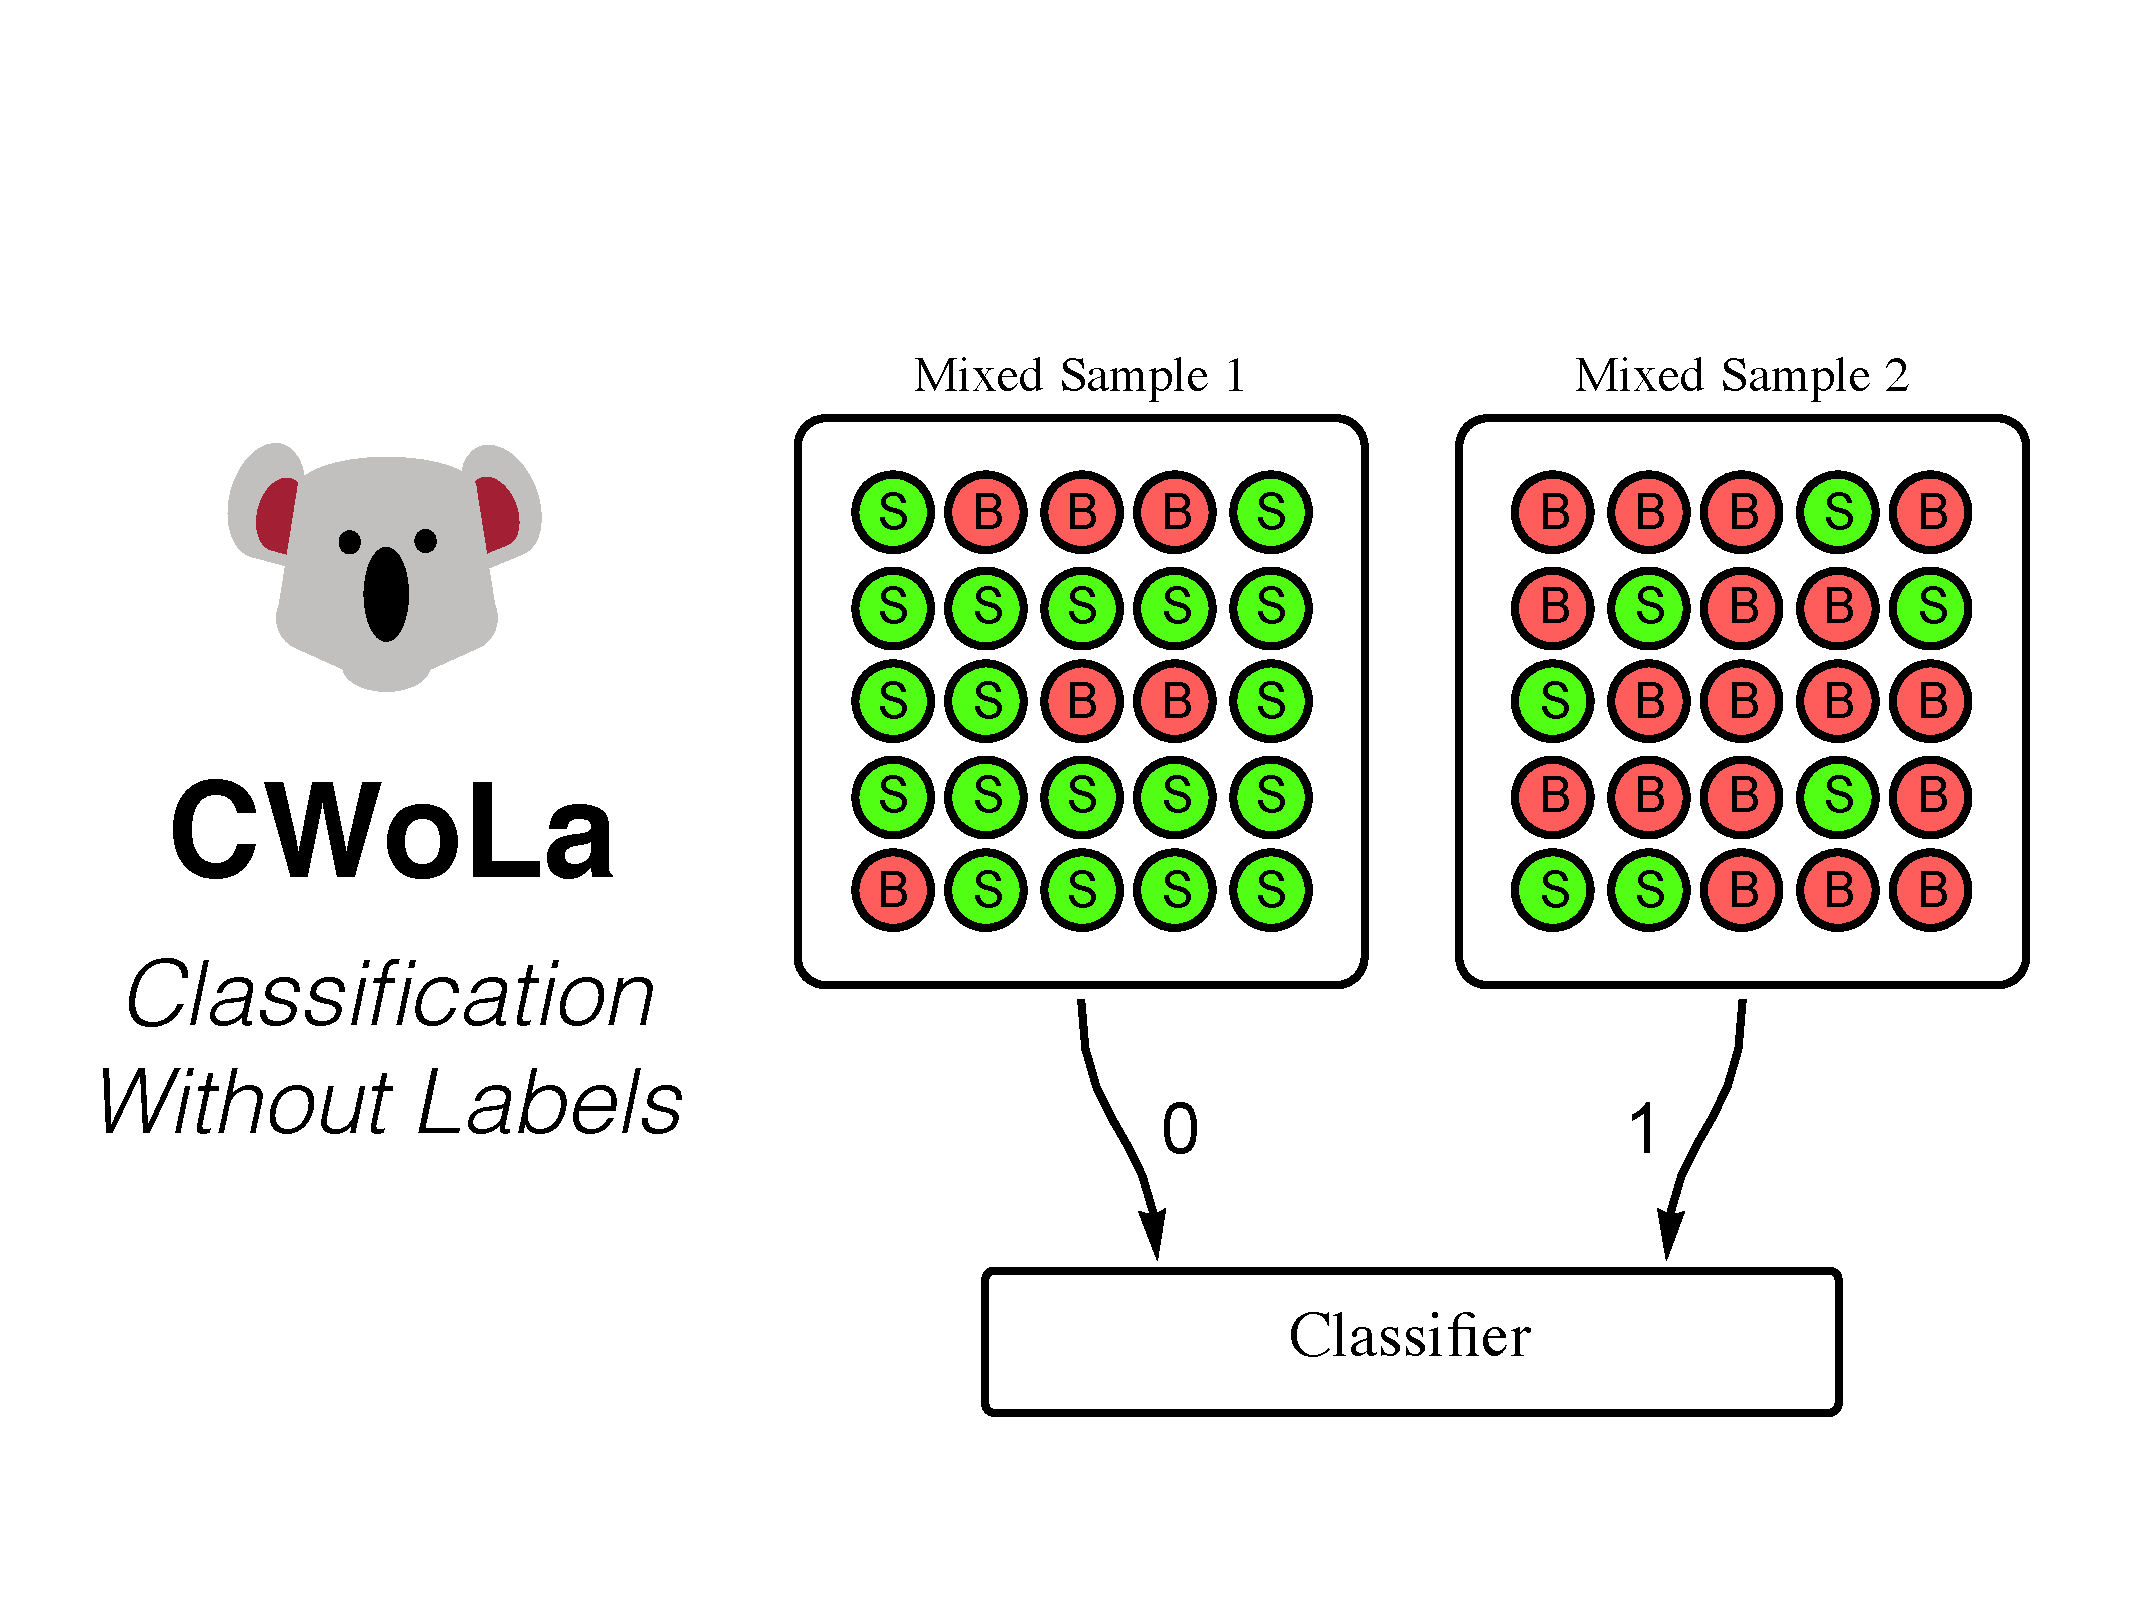
\includegraphics[width=0.6\textwidth]{figures_CWoLa/cwola.pdf}
\caption{
  Schematic of basic idea behind classification without labels (CWoLa), represented by a koala bear.
  There are two samples, each of which has a mixed but different composition of signal and background events.
  A supervised classifier is trained to distinguish between the two mixed samples.
  This same classifier is then used to distinguish between signal and background events.
  Figure adapted from~\cite{Metodiev:2017vrx}.
}
\label{fig:CWoLa:cwolasetup}
\end{figure}

It is worth noting the properties and limitations of this method.
First, the features used to distinguish between signal and background events cannot or can only be very bad at distinguishing between background events in Mixed Sample 1 and Mixed Sample 2 (and similarly for signal events, though typically the signal presence is very small in one sample and basically zero in the other, so this is not as much of a concern).
Second, the key insight is that it is okay if there is some signal in both mixed samples; however, learning is easiest when the fraction of signal between the two mixed samples differs the most.
This being said, because the classifier is trained directly on data, it avoids the first major drawback of supervised learning mentioned above, since there is no possible simulation-data difference.

As mentioned above, the second major drawback of supervised learning is that the trained classifier is only sensitive to one particular signal model.
The idea of ``CWoLa hunting''~\cite{Collins:2018epr,Collins:2019jip} is to use the CWoLa method to search for BSM physics without a particular signal model in mind.
In fact, the method learns to tag whatever signal is present in the data, allowing the search to be generically sensitive to new signals that have different distributions of whatever features are used than the background.
The setup CWoLa hunting is shown schematically in Figure~\ref{fig:CWoLa:cwolahuntingsetup}.
There is some feature $m_\text{res}$ for which the background has a smoothly falling spectrum, while the signal is narrowly peaked (\textit{resonant}) in that feature.
Two mixed samples are formed: one with values of $m_\text{res}$ centered near the potential new resonance and one using events in neighboring regions of $m_\text{res}$.
A neural network (NN) is trained to distinguish between these two mixed samples based on some other features, resulting in an overall score $y$.
The first mixed sample clearly has a higher signal fraction than the second;
and because the two mixed samples come from nearby regions of $m_\text{res}$, the difference in distributions of features in the background between the two mixed samples can be smaller than the fraction of signal times the difference in distributions between the signal and background.
Therefore, because of the principles of CWoLa, the scores from the resulting network $y$ can distinguish between signal and background events. 
In the case that in fact there was no signal in the first mixed sample, the tagger will either learn to tag randomly or learn to tag based on the minute differences in the background between the samples.
In either case, after tagging based on the output $y$, the combined spectrum of $m_\text{res}$ can be fit with a smooth function - if indeed there was a signal, there will be a bump in the $m_\text{res}$ spectrum; while if there was no signal, the background should remain smooth, even if the network learned to tag some differences in the background\footnote{This is why it is key to use neighboring regions on both sides. The prevention of background sculpting is a major consideration in this analysis, as discussed in more detail in Section~\ref{sec:CWoLa:Analysis:Overview}.}.
This process is then repeated for different regions of $m_\text{res}$ in order to be sensitive to a broad spectrum of BSM masses.
One of the key aspects of this technique is a nested cross-validation procedure, which prevents overtraining in the case of no signal presence.

\begin{figure}
\centering
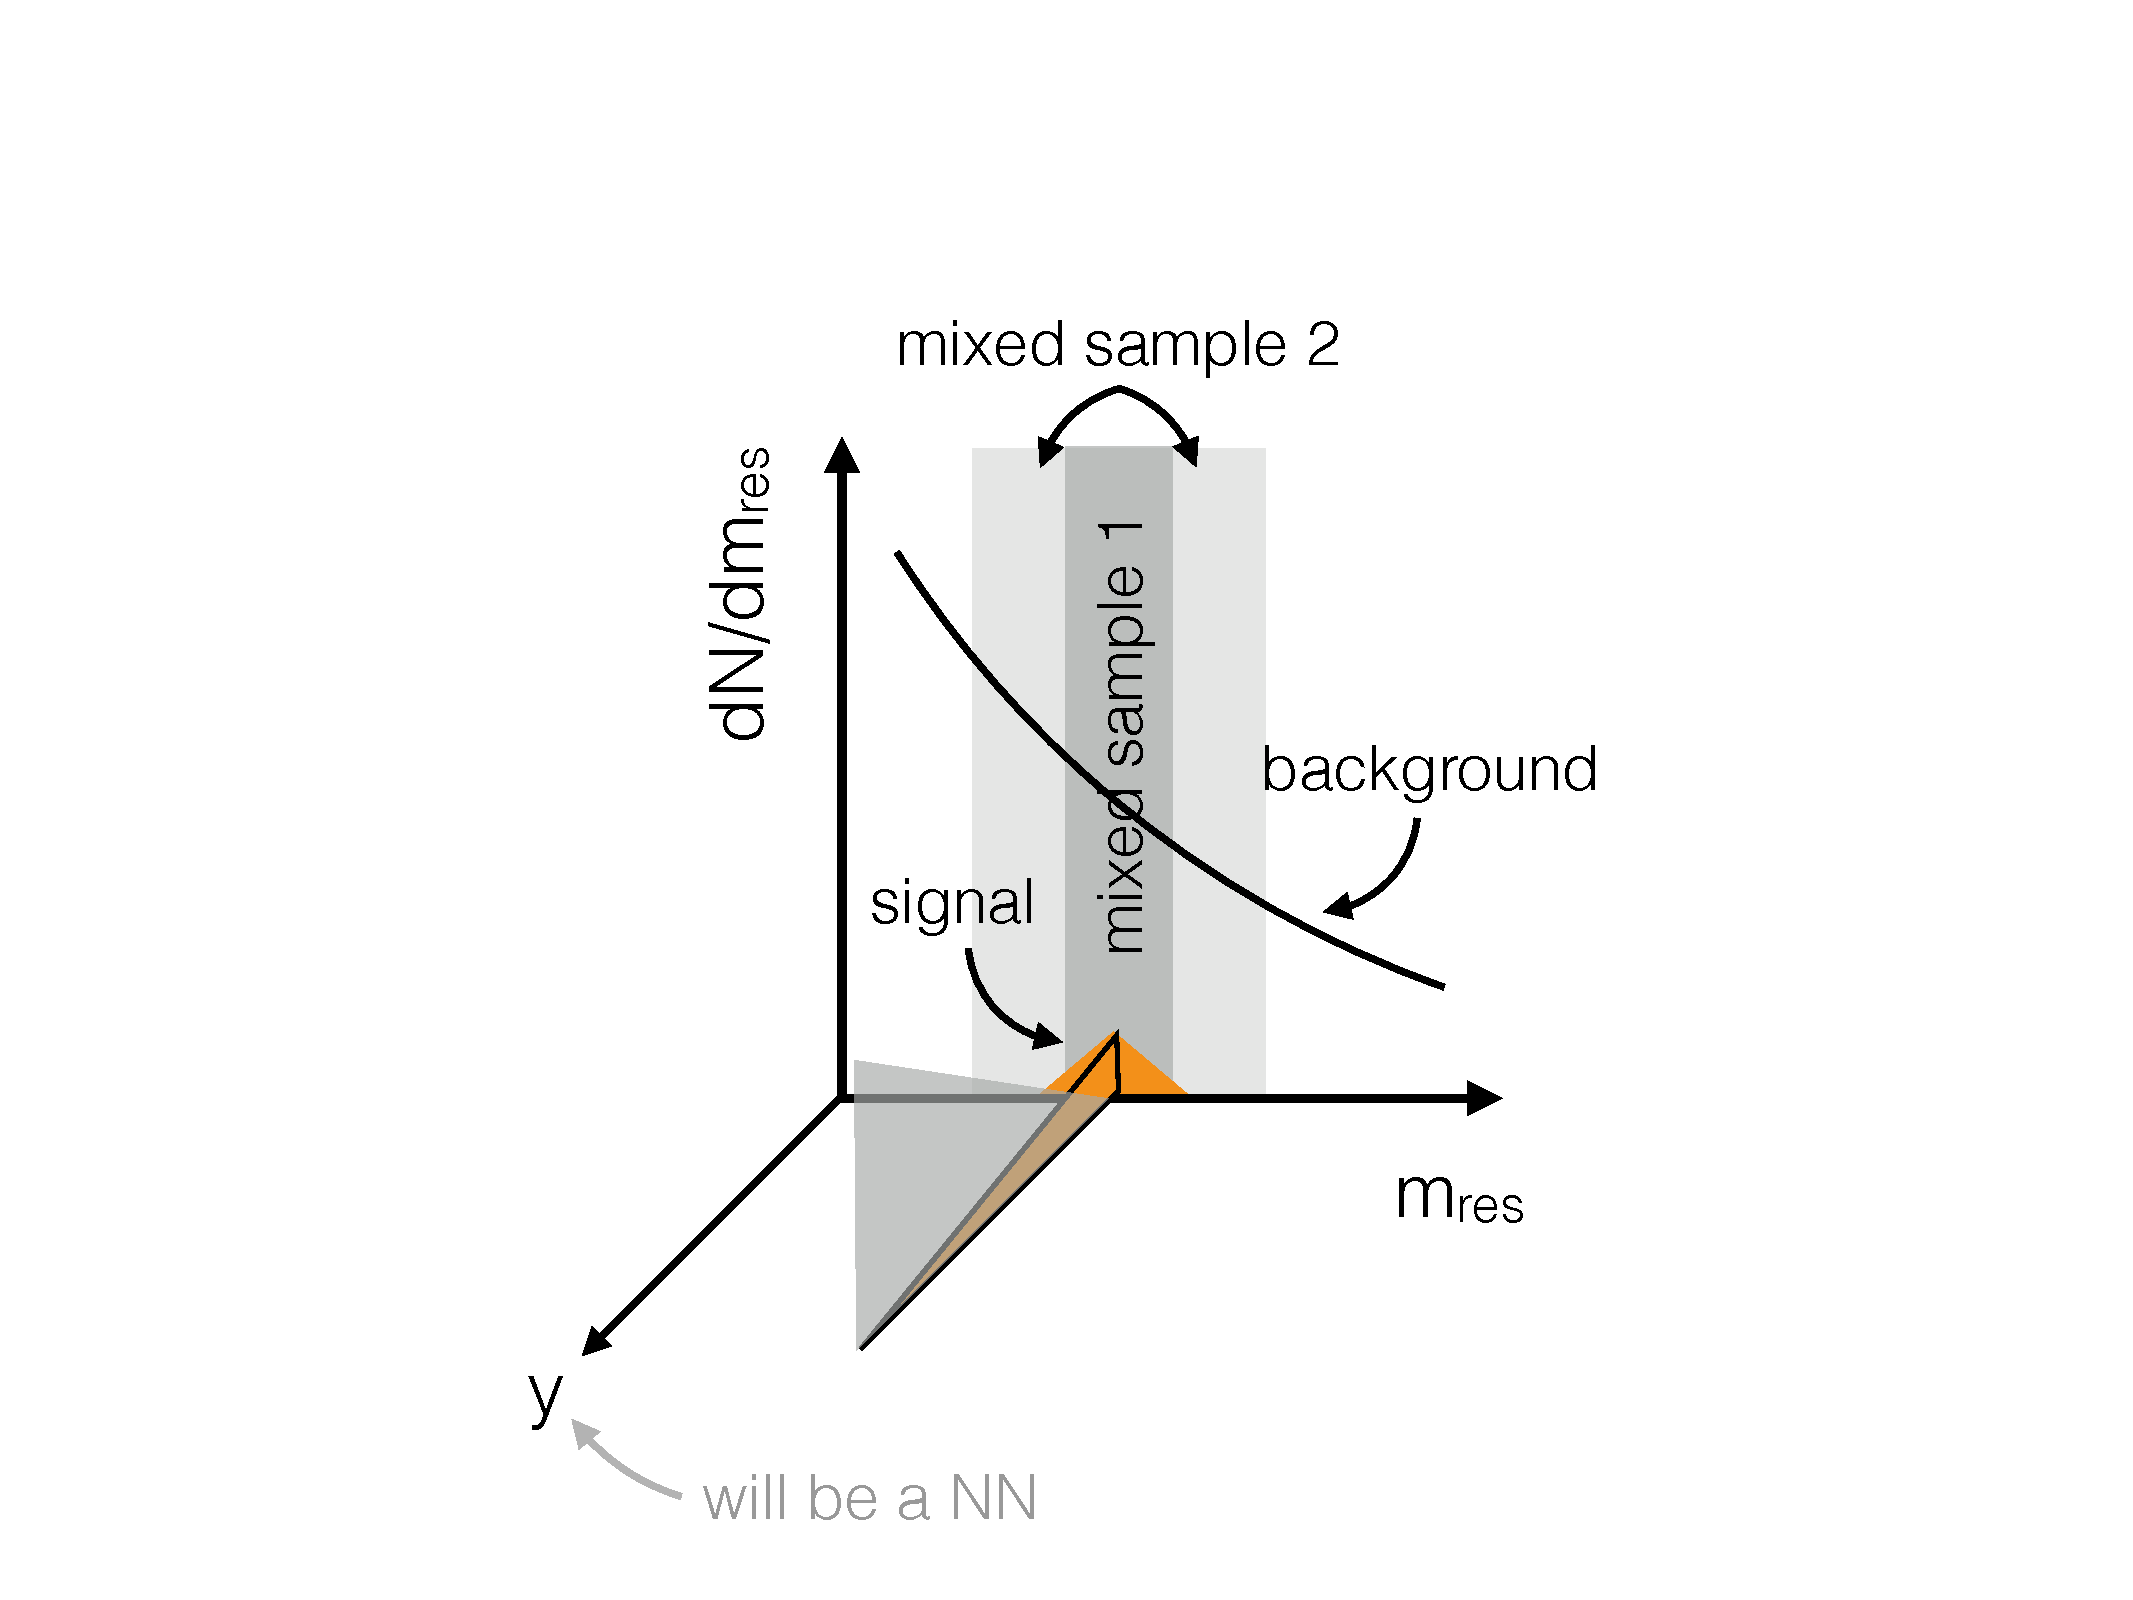
\includegraphics[width=0.5\textwidth]{figures_CWoLa/cwolahuntingsetup.pdf}
\caption{
  A schematic for the setup of CWoLa hunting.
  The background has a smoothly falling spectrum in some feature $m_\text{res}$, while the signal is narrowly peaked (resonant) in that feature.
  A network is trained to distinguish between a narrow region of $m_\text{res}$ in which the signal lies from its neighboring regions.
  Because of the principles of CWoLa, the scores from the resulting network $y$ can distinguish between signal and background events. 
  Figure adapted from~\cite{NPKI_CWoLa_Hunting}.
}
\label{fig:CWoLa:cwolahuntingsetup}
\end{figure}

This and other key aspects are discussed in the following Section, which lays out the assumptions and specifics of this analysis based on the above ideas with $m_\text{res}=m_{JJ}$.

\clearpage
\subsection{Analysis Strategy}
\label{sec:CWoLa:Analysis:Overview}
This analysis utilizes the concept of Classification Without Labels (CWoLa) described in Section~\ref{sec:CWoLa:schematic} in order to be sensitive to a broad class of non-SM models of the form $A\rightarrow BC$, with $A$ massive and on-shell, and the decay products of $B$ and $C$ reconstructed as large-$R$ jets in the ATLAS calorimeter.
In these models, the reconstructed dijet mass $m_{JJ}$ will show a peak near the mass of the $A$, with width determined by the dijet mass resolution.
There are two key assumptions that enable this analysis to be sensitive to these models.
\begin{enumerate}
  \item \textbf{(Assumption 1)} One or both of the jets reconstructed from the $B$ and $C$ decays have features, e.g. in their substructure, which differ from the background composition (i.e., non-resonant dijet events from QCD and other SM processes), so that these jets can be tagged in order to increase the signal to background ratio of the signal $m_{JJ}$ peak over the background shape. \label{ass1}
  \item \textbf{(Assumption 2)} After tagging on these features, the background $m_{JJ}$ remains smooth, so that a fit to the background $m_{JJ}$ spectrum does not indicate a potential discovery via a bump in the $m_{JJ}$ spectrum. \label{ass2}
\end{enumerate}
In particular, clearly one of the features that differs between the signal and the background composition is $m_{JJ}$ itself; if $m_{JJ}$ is used as a feature, or if jet features that allow reconstruction of $m_{JJ}$ are used, then Assumption~\ref{ass2} is violated, because after tagging on this feature the $m_{JJ}$ spectrum in the background will no longer be smooth.
Therefore some effort must be put into choosing features that will not violate Assumption~\ref{ass2}, and into validating that the assumption is not violated once the features are chosen.

Under these assumptions, the outline of the analysis is as follows.
\begin{enumerate}
  \item Select events in which at least two large-$R$ jets are reconstructed, and in these events form the dijet invariant mass, $m_{JJ}$, and record some relevant jet features $X$.\label{step1}
  \item Partition the $m_{JJ}$ spectrum into discrete, monotonically increasing bins.\label{step2}
  \item Label one of these bins the \textit{signal region}, and the bins on either side in $m_{JJ}$ space the \textit{sideband regions}.~\label{step3}
  \item Train a neural network (NN) to distinguish between the signal region and the sideband regions based on the chosen features $X$.
    There are three possibilities of what the network learns, based on where the true signal lies relative to the signal region.
    \begin{enumerate}
      \item If the signal mass peak happens to lie in the signal region, then the signal fraction in the signal region will be higher than in the sideband regions, and the network will learn that it can identify some events in the signal region by tagging the true signal; i.e., the network will learn how to tag signal events.
        This process is what is referred to as CWoLa.\label{case1}
      \item If the signal mass peak happens to lie in one of the sideband regions, then the signal fraction in the signal region will be lower than in the sideband regions, and the network will learn to identify some events in the sideband region by tagging the true signal; i.e., the network will learn how to anti-tag signal events.\label{case2}
      \item If the signal mass peak does not lie in the signal region or sideband regions, or if there is no signal at all, then the network will learn to distinguish between the background events in the signal and sideband regions based on the features $X$, as far as such correlations exist.\label{case3}
    \end{enumerate}
    Note that, in Cases~\ref{case1} and~\ref{case2}, the network is sensitive to both the difference in the distribution of the features $X$ between the signal and the background, and to the differences between the background in the signal region and the background in the sideband regions.
    In order to allow the network to focus on tagging the signal versus the background, the sideband regions are chosen to be adjacent to the signal region in kinematic space so that the difference in the features in the background between the signal and sideband regions is minimzed.
  \label{step4}
  \item Tag events by choosing events with high neural network output.
    In Case~\ref{case1}, the neural network is a signal tagger, so the signal-to-background ratio increases, in particular increasing the significance of the signal peak over the background $m_{JJ}$ shape. 
    In Case~\ref{case2}, the network anti-tags signal, and in Case~\ref{case3}, the network tags only differences in the background between signal and sideband regions; in either case, the signal-to-background ratio after tagging is small or zero.
  \label{step5}
  \item Fit to the $m_{JJ}$ shape after tagging.
    Because of Assumption~\ref{ass2}, the background spectrum is smooth after tagging.
    In Case~\ref{case1}, there will be a bump in the $m_{JJ}$ spectrum in the signal region due to the presence of signal, allowing the potential of a discovery of this signal.
    In Cases~\ref{case2} and~\ref{case3}, there will be little to no signal, so there will be no bump in the $m_{JJ}$ spectrum, and the spectrum fit will not indicate the discovery of a signal.
    \label{step6}
  \item Repeat Steps~\ref{step3}-\ref{step6} with each possible signal region bin.
    If there is any true signal, then the signal will lie in one of the signal region bins, and Case~\ref{case1} will be true in that bin, allowing discovery of this signal.
    If there is no true signal, then in each signal region bin Case~\ref{case3} will be true, thus indicating no discovery over the whole $m_{JJ}$ range.
\end{enumerate}
Since there is a difference in the observed outcomes between the case where there is presence of signal and when there is no signal, limits can be set on specific signal models based on what would have been observed if those signals were present.

Since the network learns what features distinguish the signal from the background automatically, this analysis is sensitive to a wide range of possible signal distributions of these features, and thus the analysis can be sensitive to a wide range of signal models without paying the price of a look-elsewhere effect that a dedicated search for each one of these signal models would entail.

Furthermore, since the network learns the features that distinguish the signal from the background directly from data, the tagger does not need to be calibrated to account for differences between simulation and background; this removes a source of uncertainty relative to a dedicated search with a tagger trained to distinguish between signal and background in simulation.

\clearpage
\subsection{Blinding and Validation Procedure}
\label{sec:CWoLa:blinding}
Validating the analysis in a blinded region of the data is a challenge for this analysis.
In a typical analysis, after running the analysis entirely in simulation, some validation region is defined with orthogonal cuts with low signal efficiency in order to validate the analysis.
This validation region is used to either do data/MC comparisons to verify that the simulation is describing the background adequately or to perform in situ checks of the assumptions of the analysis.
For example, in the search described in Chapter~\ref{ch:HBSM}, the background is estimated in a data-driven way with an A/B/C/D matrix of regions; the highest signal efficiency is expected in region D.
The assumption of the A/B/C/D method (that the ratio of events in B/A is the same as in D/C in the background) is verified both in simulations of the background and in a data validation region, inverting the $m_{gg\gamma\gamma}$ cut.

In this analysis, the original event selection (Analysis Step~\ref{step1}) is inclusive and minimal, in order to be sensitive to a broad class of new models.
The event selection learned by the NN depends on the data, so there is no way to construct an orthogonal signal-deficient region ahead of time.
In Analysis Step~\ref{step5}, only events with some high NN score are chosen, so one idea is to use the events with lower NN scores for validation.
However, this does not clearly work - if selecting only events that the NN assigned \textit{low} scores, then in Case~\ref{case2}, where the network has anti-tagged the signal, this selection would actually have a high signal efficiency, defeating the purpose of the validation region.
Another option is to select only events with \textit{average} scores, i.e. close to the median NN output.
However these events are exactly those for which the NN has decided it cannot distinguish between the signal and sideband regions, so that even if Assumption~\ref{ass2} were being violated in general by the NN selection, for these events the Assumption would \textit{not} be violated, again defeating the purpose of a validation region.
These ideas and others for constructing a validation sample are explored in Appendix~\ref{app:CWoLa:validation_alternate}.

In light of these considerations, the event selection is given one additional non-trivial selection, a maximum rapidity difference between the two jets in the event; and the validation region is defined to be the inverse of this.
This rapidity selection is also present in the inclusive dijet search~\cite{Aad:2019hjw} and in the all-hadronic diboson resonance search~\cite{Aad:2019fbh}, two analyses which are sensitive to similar signals and also aim to be inclusive in their searches.
This selection both suppresses contributions from $t$-channel QCD dijet production, while remaining efficient on $A\rightarrow BC$ signals.
The distribution of the rapidity difference in the background simulation can be seen in Figure~\ref{fig:CWoLa:bkg_rapdiff}, and the distributions in various signal models can be seen in Figure~\ref{fig:CWoLa:sig_rapdiff}.

\begin{figure}[htbp]
  \centering 
  \subfloat[]{\includegraphics[width=0.45\textwidth]{figures_CWoLa/{jet_rapdiff_log_bn04_4.10.19}.pdf}}
  \subfloat[]{\includegraphics[width=0.45\textwidth]{figures_CWoLa/{jet_rapdiff_log_bn510_4.10.19}.pdf}}
  \caption{Distribution of $|y_1-y_2|$ in the background simulation, broken down by the $m_{JJ}$ region, as described in Section~\ref{sec:CWoLa:binning}. (a) $m_{JJ}$ regions 0-4; (b) $m_{JJ}$ regions 5-9. The green line indicates the cut at 1.2 (Section~\ref{sec:CWoLa:eventselection}).}
\label{fig:CWoLa:bkg_rapdiff}
\end{figure}

\begin{figure}[htbp]
  \centering 
  \subfloat[]{\includegraphics[width=0.45\textwidth]{figures_CWoLa/{jet_rapdiff_log_Wprime_WZqqqq_M3000_m200_m200_4.10.19}.pdf}}
  %\subfloat[]{\includegraphics[width=0.45\textwidth]{figures_CWoLa/{jet_rapdiff_log_Wprime_WZqqqq_M6000_m200_m200_4.10.19}.pdf}}
  \caption{Distribution of $|y_1-y_2|$ for a signal model with ($m_A,m_B,m_C=3000,200,200$ GeV).
    %(a) ($m_A,m_B,m_C=3000,200,200$ GeV);
    %(b) ($m_A,m_B,m_C=6000,200,200$ GeV).
    The green line indicates the selection at 1.2 (Section~\ref{sec:CWoLa:eventselection}).}
\label{fig:CWoLa:sig_rapdiff}
\end{figure}

The validation and unblinding procedure is then as follows:
\begin{enumerate}
\item Run the full method in simulation.  These results are presented in Section~\ref{sec:CWoLa:simulation_analysis}.  Two challenges with this validation are (i) we have less simulation than data and (ii) the simulated events are weighted.  The latter can be challenging for our training procedure and is not an issue for the real data version of the analysis. This step is referred to as the ``simulation'' or ``MC'' analysis.
\item Proceed to run the full method on data where the rapidity gap cut is inverted.  Any $s$-channel model will have a reduced cross-section while the background rate increases.  This is discussed in Section~\ref{sec:CWoLa:val_analysis} and allows us to run the full procedure on data where we do not expect to see any signal. This step is referred to as the ``inverted rapidity cut'', ``data validation'', or simply ``validation'' analysis, as it serves as the main validation in data before the full unblinded analysis.
\item Run the method on the full dataset (with the uninverted rapidity gap cut).  The results of this are reported in Section~\ref{sec:CWoLa:unblinded}. This step is referred to as the ``uninverted'', ``unblinded'', ``signal selection'', or simply ``full'' analysis.
\end{enumerate}

The development of this analysis occurred by progressing through each of these steps in turn, and though overall most of the analysis remained the same between each of the steps, naturally some details changed after learning things at various steps of the validation.
The details of the analysis outlined in Section~\ref{sec:CWoLa:analysis_details} apply to each of these steps, but are clear about where they are different.
In particular, the fitting process (Analysis Step~\ref{step6}) went through multiple iterations before settling on the final procedure.
In general, doing a parametric background fit on large datasets tends to be a key challenge;
this challenge was compounded due to the effective statistics of the background in each of these steps, which is expanded on below.

The effective statistics of the inverted sample compared with the nominal sample and the simulation are presented in Figure~\ref{fig:CWoLa:effectivestats}\footnote{Also given for good measure are the statistics for 3.2\ifb, which corresponds to the 2015 LHC dataset.}.
The binnings presented there are those defined in Section~\ref{sec:CWoLa:binning}, and given in Table~\ref{tab:mjj_bins}.
For the simulation, the effective statistics is defined as the inverse of the sum of the squares of the normalized event weights.
For the central dataset, the MC statistics are relatively uniform in $m_{JJ}$ and there are only more effective events past the third bin, with boundaries at $1.90 \le m_{JJ} < 2.28$ TeV.
Even in the fourth bin ($2.28 \le m_{JJ} < 2.74$ TeV), there are events with a large weight, which makes the training and fitting unrealistic.

For the inverted dataset, the problem is much more severe because for a fixed $m_{JJ}$, lower $p_T$ jets can contribute than for the central dataset.
For the full Run 2 statistics, the MC has the same number of weighted events only by the eighth bin($4.73 \le m_{JJ} < 5.68$ TeV).

\begin{figure}[h!]
\centering
\subfloat[]{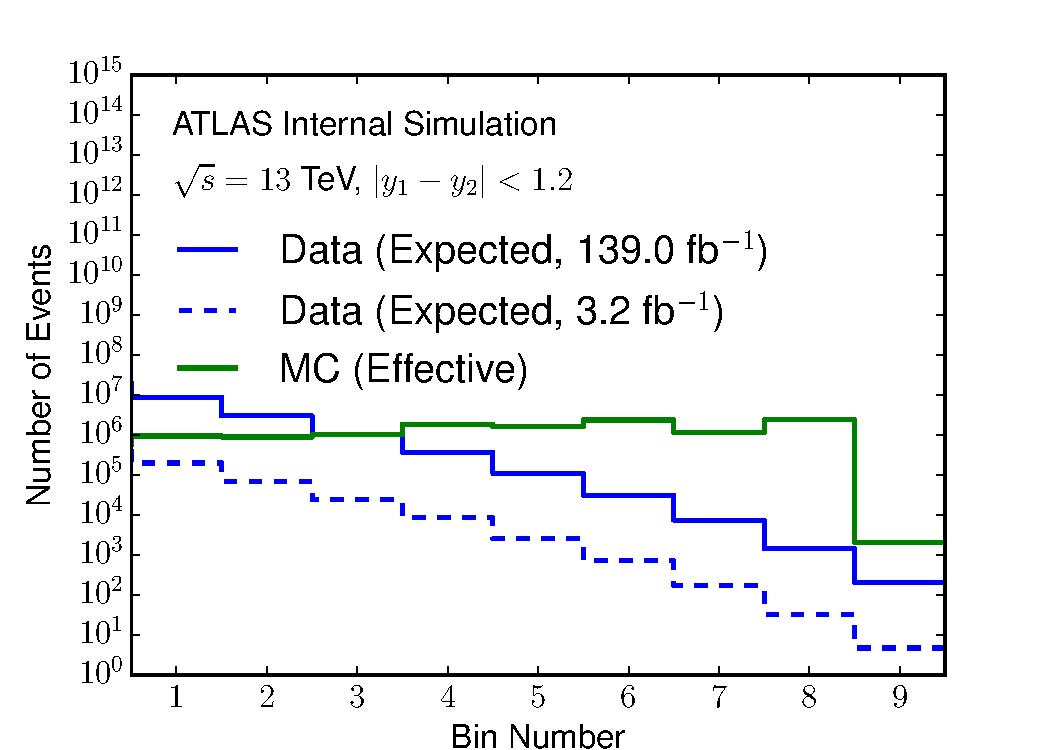
\includegraphics[width=0.45\textwidth]{figures_CWoLa/MCstats_4_10_19.pdf}}
\subfloat[]{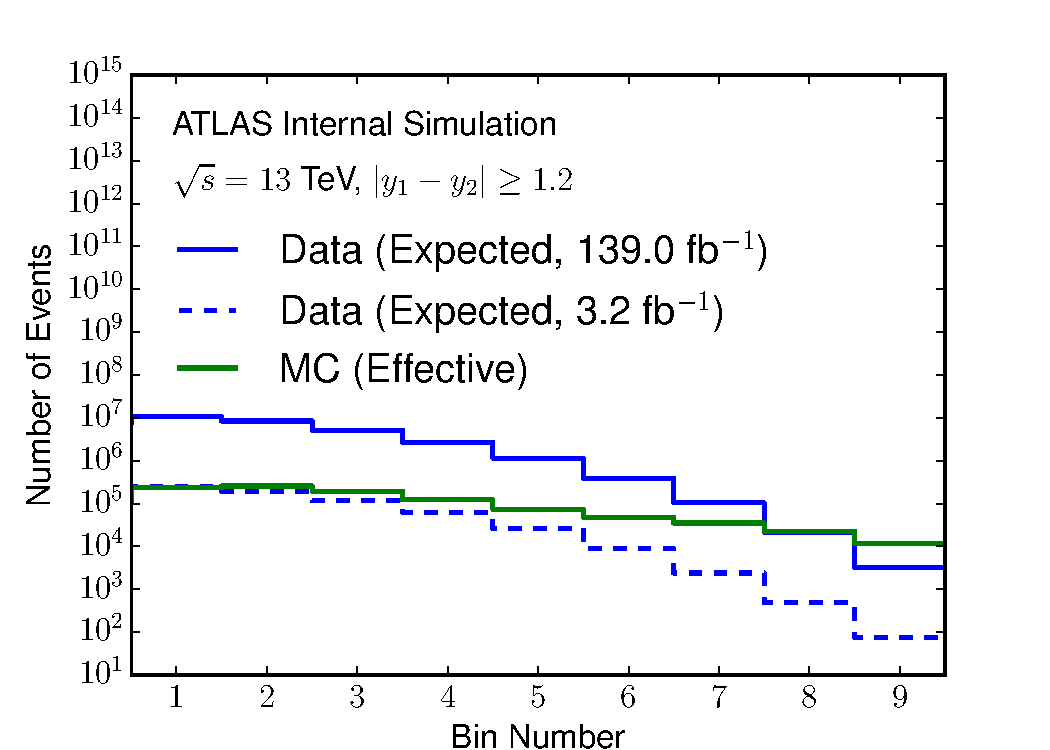
\includegraphics[width=0.45\textwidth]{figures_CWoLa/MCstats_yinvert_4_10_19.pdf}}
\caption{The effective statistics for the nominal rapidity difference (a) and the inverted one (b) for MC and data and for different integrated luminosities.}
\label{fig:CWoLa:effectivestats}
\end{figure}

The inverted dataset has about ten times more events than the nominal rapidity difference dataset above about 3 TeV, which can be seen in Figure~\ref{fig:CWoLa:invertedcutratio}.
In order for the inverted dataset to have comparable statistics to the nominal dataset for testing our methodology, random sampling without replacement is used to reduce the dataset.
The random sampling rate is determined from a fit to the ratio of efficiencies for the two rapidity differences cuts (also shown in Figure~\ref{fig:CWoLa:invertedcutratio})
\footnote{In principle, by looking at this distribution, we have unblinded the full dataset with no NN cut.  However, we have not examined this distribution in detail and have not performed any statistical tests on the quality of the fit.  It actually may be easier to do the bump hunt in this ratio, which is relatively flat, but this is left for future studies.}.

\begin{figure}[h!]
\centering
\includegraphics[width=0.45\textwidth]{figures_CWoLa/{yinvert_eff_fit_11.2.19}.pdf}
\caption{The ratio of efficiencies for the two rapidity differences cuts.  A fit shown with a dashed line is the sum of two power law functions.  Note that these are data plots and not simulation.}
\label{fig:CWoLa:invertedcutratio}
\end{figure}

As will be mentioned in Section~\ref{sec:CWoLa:fitting}, each analysis imposes a cut of $m_{JJ}>1.8$ TeV for the fitting.
For the simulation analysis, as mentioned above, the effective MC statistics are only reliable above around that value.
For the data analyses, this cut results mainly from the finding that the fitting procedure simply is not sufficient to describe the background shape for the high numbers of events seen below that cut\footnote{A more sophisticated (possibly non-parametric) fitting procedure may be able to extend the search to lower values in the future.}.
However, it is also the case that the inverted rapidity selection provides multiple copies of independent datasets to test the analysis when the ratio of efficiencies is $<\frac{1}{2}$;
in particular, the ratio of efficiencies is $<\frac{1}{3}$ (so $3$ statistically independent copies) for $m_{JJ}>\sim 1.8$ TeV, which was useful for testing the statistical properties of the fitting.

\clearpage
\section{Analysis Details}
\label{sec:CWoLa:analysis_details}

\subsection{Event Selection}
\label{sec:CWoLa:eventselection}
The following can be considered an explication of the event selection mentioned in Analysis Step~\ref{step1}.

As mentioned in Section~\ref{sec:CWoLa:data}, data are collected using the lowest available unprescaled single-jet trigger.

%For both data and simulation, the EXOT3 derivation is used, which requires at least two \\ \texttt{AntiKt10LCTopoTrimmedPtFrac5SmallR20} jets with $\pt>100$ GeV, $|\eta|<2.8$, and (uncalibrated) $m>30$ GeV if the jet $\pt$ is less than 1000 GeV.

This analysis uses anti-$k_t$, $R=1.0$ jets reconstructed from topoclusters with the local cluster weighting scheme (LCW)~\cite{Aad:2016upy}.
The jets are trimmed~\cite{Krohn:2009th} using using the parameters $f_\text{cut} = 5\%$ and $R_\text{sub} = 0.2$.
A Monte Carlo-based particle-level calibration is then applied to the jets used in this analysis~\cite{Aaboud:2018kfi}.
It corrects on average the reconstructed mass and $p_T$ of the jets to their true values.
The \textit{combined mass} measurement is used, which combines measurements from the tracking system and the calorimeter; including this information has been shown to have better mass resolution, especially at high jet $\pt$~\cite{ATLAS-CONF-2016-035}.

The offline selection that is made on top of the selection from the derivation is intended to be as fully inclusive as possible to prospective signal models, while remaining on the plateau of the turn-on for the trigger.

Each event is required to have at least two large-$R$ jets with calibrated $\pt>200$ GeV
\footnote{Jet calibrations for large-radius jets only go to 200 GeV.
%In any case, the number of jets with $\pt$ between 100 and 200 GeV is negligible: 0.1\% for $m_{JJ} > 1.8$ TeV.
%The simulation and validation analyses do not remove these as they are already done and nothing noticeable will change by removing them (at the expense of a lot of additional work).  They are removed for the unblinded nominal data analysis.
}
and $|\eta|<2.0$, and with at least one such jet with calibrated $\pt>500$ GeV.
This offline threshold has been shown to be fully efficient with respect to the trigger selection~\cite{Adorni:2647394}.
There is no explicit lepton overlap removal or veto.

Only the two jets with highest $\pt$ in the event are used in this analysis, and the remaining jets are discarded.
For each jet $j=1,2$, the four-momentum $p^\mu_j$ recorded, in particular the jet mass $m_j^2 = (p^\mu_j)^2$.
As mentioned in Section~\ref{sec:CWoLa:blinding}, a selection is placed on the rapidity difference, $|y_1-y_2|<1.2$.
%The distribution of the rapidity difference in the background simulation can be seen in Figure~\ref{fig:CWoLa:bkg_rapdiff}, and the distributions in various signal models can be seen in Figure~\ref{fig:CWoLa:sig_rapdiff}.

The jets are ordered by their mass, so that $m_1 \ge m_2$.
In order to suppress background and therefore increase sensitivity to massive signal objects, a minimum cut $m_1$, $m_2 > 30$ \GeV{} is applied.
Also, in order to make the kinematic region in which the learning is applied definite, as discussed in Section~\ref{sec:CWoLa:features}, a maximum cut $m_1$, $m_2 < 500$ \GeV{} is applied.

Typically the dijet invariant mass $m_{JJ}$ would be defined as in terms of the sum of the four-momenta of the two jets, $m_{JJ}^2 = (p^\mu_1+p^\mu_2)^2 = m_1^2+m_2^2+2\left(E_1E_2-\vec{p}_1\cdot\vec{p}_2\right)$, with $E^2 = |\vec{p}|^2+m^2$ and $|\vec{p}| = p_T\cosh(\eta)$.
In this analysis the dijet invariant mass is defined slightly differently: in order to reduce correlations between the features used in the neural network ($m_1,m_2$) and the final $m_{JJ}$ value, the dijet invariant mass is formed by setting all $m_i$ to zero: $m_{JJ}^2 \equiv 2\left(|\vec{p}_1||\vec{p_2}|-\vec{p}_1\cdot\vec{p}_2\right)$.
This new definition removes all correlations between $m_{JJ}$ and $m_1,m_2$ except for those arising from indirect correlations between the jet $m$ and the jet $p_T$ and $\eta$.
In practice this is a very small change, because the jets in this analysis typically have energies much larger than their masses, and so the new definition gives almost the same value for the invariant mass.
As will be discussed in Section~\ref{sec:CWoLa:binning}, a selection is applied on the dijet invariant mass of $1.1 \le m_{JJ} < 8.17$ TeV.
As will be discussed in Section~\ref{sec:CWoLa:fitting}, effectively a selection of $1.8 \le m_{JJ}$ TeV is applied as the fitting range.

These selections are summarized in Table~\ref{tab:event_selection}.
\begin{table}[htbp]
  \begin{center}
    \caption{Jet selection. The $m_{JJ}$ selection is indicated for the $m_{JJ}$ bins (Section~\ref{sec:CWoLa:binning}) and also for the fitting range (Section~\ref{sec:CWoLa:fitting}).}
  \label{tab:event_selection}
    \begin{tabular}{c c}
      \hline
      Observable & Selection \\
      \hline
      $p_T$ & $>500$ GeV (leading), $>200$ GeV (subleading) \\
      $|\eta|$ & $<2.0$ \\
      $|y_1-y_2|$ & $<1.2$ \\
      $m$ & $> 30$ GeV, $<500$ GeV \\
      $m_{JJ}$ (bins) & $\ge 1.1$ TeV, $<8.17$ TeV \\
      $m_{JJ}$ (fitting) & $\ge 1.8$ TeV \\
      \hline
    \end{tabular}
  \end{center}
\end{table}

The cutflow of these selections on the signal samples is given in Table~\ref{tab:cutflow_signal}.
\begin{table}[htbp]
  \begin{adjustwidth}{-2cm}{-2cm}
  \begin{center}
    \caption{Signal sample efficiency with selections up to and including given selection. All selections are given in Section~\ref{sec:CWoLa:eventselection}. The jet selections are summarized in Table~\ref{tab:event_selection}. The $m_{JJ}$ selection is included for the binning selection of $1.1 \le m_{JJ} < 8.17$ TeV and for the additional selection from the fitting of $1.8 \le m_{JJ}$ TeV.}
  \label{tab:cutflow_signal}
    \begin{tabular}{c c c c c c c c c}
      \hline
      $(m_A,m_B,m_C)$ [\GeV] & Derivation & Trigger & \pt & $|\eta|$ & $|y_1-y_2|$ & $m$ & $m_{JJ}$ (bins) & $m_{JJ}$ (fitting) \\
      \hline
      (3000,80,80)   & 1.00 & 0.90 & 0.85 & 0.85 & 0.64 & 0.63 & 0.62 & 0.59 \\
      (3000,80,200)  & 1.00 & 0.91 & 0.85 & 0.85 & 0.63 & 0.62 & 0.61 & 0.58 \\
      (3000,80,400)  & 1.00 & 0.92 & 0.81 & 0.81 & 0.61 & 0.60 & 0.58 & 0.56 \\
      (3000,200,200) & 1.00 & 0.93 & 0.87 & 0.87 & 0.64 & 0.63 & 0.63 & 0.59 \\
      (3000,200,400) & 1.00 & 0.95 & 0.84 & 0.84 & 0.62 & 0.61 & 0.60 & 0.58 \\
      (3000,400,400) & 1.00 & 0.95 & 0.82 & 0.82 & 0.62 & 0.60 & 0.59 & 0.57 \\
      (5000,80,80)   & 1.00 & 0.68 & 0.58 & 0.58 & 0.44 & 0.44 & 0.42 & 0.34 \\
      (5000,80,200)  & 1.00 & 0.70 & 0.59 & 0.59 & 0.45 & 0.44 & 0.42 & 0.34 \\
      (5000,80,400)  & 1.00 & 0.78 & 0.58 & 0.58 & 0.44 & 0.43 & 0.40 & 0.34 \\
      (5000,200,200) & 1.00 & 0.75 & 0.63 & 0.63 & 0.48 & 0.47 & 0.45 & 0.37 \\
      (5000,200,400) & 1.00 & 0.82 & 0.65 & 0.65 & 0.49 & 0.48 & 0.45 & 0.39 \\
      (5000,400,400) & 1.00 & 0.88 & 0.68 & 0.68 & 0.50 & 0.48 & 0.47 & 0.43 \\
      \hline
    \end{tabular}
  \end{center}
  \end{adjustwidth}
\end{table}

\clearpage
\subsection{Binning}
\label{sec:CWoLa:binning}
As mentioned in Analysis Step~\ref{step2}, the $m_{JJ}$ spectrum is binned in order to derive the signal and sideband regions.
The size of the binning is chosen to be 20\%, guided by the dijet mass resolution of the signal models.
The minimum $m_{JJ}$ value is 1.1 TeV, due to the jet and trigger selection, and the maximum value is at 8.17 TeV (the right edge of bin $10$ with 20\% bin size), above which few events are expected to be observed.
Since every event is required to lie in an $m_{JJ}$ bin, effectively an event selection is therefore applied for $1.1 \le m_{JJ} < 8.17$ TeV.
The bin definitions are given in Table~\ref{tab:mjj_bins}.

\begin{table}[htb]
  \centering
  \caption{\label{tab:mjj_bins} $m_{JJ}$ bin definitions.}
  \begin{tabular}{c c}
    \hline
    Bin & Definition  \\ \hline
    0 & $1.10 \le m_{JJ} < 1.32$ TeV \\
    1 & $1.32 \le m_{JJ} < 1.58$ TeV \\
    2 & $1.58 \le m_{JJ} < 1.90$ TeV \\
    3 & $1.90 \le m_{JJ} < 2.28$ TeV \\
    4 & $2.28 \le m_{JJ} < 2.74$ TeV \\
    5 & $2.74 \le m_{JJ} < 3.28$ TeV \\
    6 & $3.28 \le m_{JJ} < 3.94$ TeV \\
    7 & $3.94 \le m_{JJ} < 4.73$ TeV \\
    8 & $4.73 \le m_{JJ} < 5.68$ TeV \\
    9 & $5.68 \le m_{JJ} < 6.81$ TeV \\
    10 & $6.81 \le m_{JJ} < 8.17$ TeV \\
    \hline
  \end{tabular}
\end{table}

The distribution of $m_{JJ}$ in the background with these bin definitions can be seen in Figure~\ref{fig:CWoLa:bkg_mjj}.
It can be seen that the distribution of $m_{JJ}$ in the background before any cuts is smooth, with no bumps indicating possible discoveries.
\begin{figure}[htbp]
  \centering 
  \subfloat[]{\includegraphics[width=0.6\textwidth]{figures_CWoLa/{mjj_loglog_4.10.19}.pdf}}
  \caption{Distribution of $m_{JJ}$ in the background MC. The green lines indicate the bin edges of $m_{JJ}$ regions 0-10.}
\label{fig:CWoLa:bkg_mjj}
\end{figure}

The distributions of $m_{JJ}$ in a variety of signal models are plotted in Figure~\ref{fig:CWoLa:sig_mjj}.
It can be seen that the mass of the signal object, $m_A$, is well-reconstructed as $m_{JJ}$, with significant tails at lower $m_{JJ}$ values.
The resolution of $m_A$ with $m_{JJ}$ is roughly 20\%, which guides the sizing of the binning, as mentioned above.

\begin{figure}[htbp]
  \centering 
  \subfloat[]{\includegraphics[width=0.3\textwidth]{figures_CWoLa/{mjj_loglog_vlines_Wprime_WZqqqq_M3000_m80_m80_1.14.20}.pdf}}
  \subfloat[]{\includegraphics[width=0.3\textwidth]{figures_CWoLa/{mjj_loglog_vlines_Wprime_WZqqqq_M3000_m80_m200_1.14.20}.pdf}}
  \subfloat[]{\includegraphics[width=0.3\textwidth]{figures_CWoLa/{mjj_loglog_vlines_Wprime_WZqqqq_M3000_m80_m400_1.14.20}.pdf}}\\
  \subfloat[]{\includegraphics[width=0.3\textwidth]{figures_CWoLa/{mjj_loglog_vlines_Wprime_WZqqqq_M3000_m200_m200_1.14.20}.pdf}}
  \subfloat[]{\includegraphics[width=0.3\textwidth]{figures_CWoLa/{mjj_loglog_vlines_Wprime_WZqqqq_M3000_m200_m400_1.14.20}.pdf}}
  \subfloat[]{\includegraphics[width=0.3\textwidth]{figures_CWoLa/{mjj_loglog_vlines_Wprime_WZqqqq_M3000_m400_m400_1.14.20}.pdf}}\\
  \subfloat[]{\includegraphics[width=0.3\textwidth]{figures_CWoLa/{mjj_loglog_vlines_Wprime_WZqqqq_M5000_m80_m80_1.14.20}.pdf}}
  \subfloat[]{\includegraphics[width=0.3\textwidth]{figures_CWoLa/{mjj_loglog_vlines_Wprime_WZqqqq_M5000_m80_m200_1.14.20}.pdf}}
  \subfloat[]{\includegraphics[width=0.3\textwidth]{figures_CWoLa/{mjj_loglog_vlines_Wprime_WZqqqq_M5000_m80_m400_1.14.20}.pdf}}\\
  \subfloat[]{\includegraphics[width=0.3\textwidth]{figures_CWoLa/{mjj_loglog_vlines_Wprime_WZqqqq_M5000_m200_m200_1.14.20}.pdf}}
  \subfloat[]{\includegraphics[width=0.3\textwidth]{figures_CWoLa/{mjj_loglog_vlines_Wprime_WZqqqq_M5000_m200_m400_1.14.20}.pdf}}
  \subfloat[]{\includegraphics[width=0.3\textwidth]{figures_CWoLa/{mjj_loglog_vlines_Wprime_WZqqqq_M5000_m400_m400_1.14.20}.pdf}}\\
  \caption{Distribution of $m_{JJ}$ for a signal model with:\\
    (a) ($m_A,m_B,m_C=3000,80,80$ GeV);
    (b) ($m_A,m_B,m_C=3000,200,80$ GeV);\\
    (c) ($m_A,m_B,m_C=3000,400,80$ GeV);
    (d) ($m_A,m_B,m_C=3000,200,200$ GeV);\\
    (e) ($m_A,m_B,m_C=3000,400,20$ GeV);
    (f) ($m_A,m_B,m_C=3000,400,400$ GeV);\\
    (g) ($m_A,m_B,m_C=5000,80,80$ GeV);
    (h) ($m_A,m_B,m_C=5000,200,80$ GeV);\\
    (i) ($m_A,m_B,m_C=5000,400,80$ GeV);
    (j) ($m_A,m_B,m_C=5000,200,200$ GeV);\\
    (k) ($m_A,m_B,m_C=5000,400,20$ GeV);
    (l) ($m_A,m_B,m_C=5000,400,400$ GeV).
  }
\label{fig:CWoLa:sig_mjj}
\end{figure}

One thing to note about this analysis is that the binnings are fixed.
A possible issue with this is that for a signal that is found close to the edge of a bin, the NN may not learn to tag that signal because it has presence in both that bin and its sideband.
This effect is mitigated somewhat due to two factors: (1) Because the background is steeply falling, there is only a small region of $m_A$ in which the signal fraction in both a signal bin and its sideband are comparable; and (2) the NN is trained on both sidebands simultaneously, so that the signal should still be tagged when distinguishing between the signal region and the combined sidebands even if it lies on the edge.
A study of this effect is presented in Appendix~\ref{app:CWoLa:binoffset}.

\clearpage
\subsection{Features}
\label{sec:CWoLa:features}
In Analysis Step~\ref{step4}, some features $X$ are designated which, as per Assumption~\ref{ass1}, can be used to distinguish signals from the background.
In this analysis, only the masses of the two jets, $X = \{m_1,m_2\}$, are used as features.

The distributions of $m_1$ and $m_2$ in the background using the nominal simulation are plotted in various $m_{JJ}$ regions in Figure~\ref{fig:CWoLa:bkg_m1_m2}.
The distributions of $m_1$ and $m_2$ in a variety of signal models are plotted in the $m_{JJ}$ region which is most efficient on that signal in Figure~\ref{fig:CWoLa:sig_m1_m2}.
It can be seen that the masses of the signal objects, $m_B$ and $m_C$, are well-reconstructed as $m_1$ and $m_2$.

\begin{figure}[htbp]
  \centering 
  \subfloat[]{\includegraphics[width=0.3\textwidth]{figures_CWoLa/{jet1_m_jet2_m_sigR0_4.10.19}.png}}
  \subfloat[]{\includegraphics[width=0.3\textwidth]{figures_CWoLa/{jet1_m_jet2_m_sigR1_4.10.19}.png}}
  \subfloat[]{\includegraphics[width=0.3\textwidth]{figures_CWoLa/{jet1_m_jet2_m_sigR2_4.10.19}.png}}\\
  \subfloat[]{\includegraphics[width=0.3\textwidth]{figures_CWoLa/{jet1_m_jet2_m_sigR3_4.10.19}.png}}
  \subfloat[]{\includegraphics[width=0.3\textwidth]{figures_CWoLa/{jet1_m_jet2_m_sigR4_4.10.19}.png}}
  \subfloat[]{\includegraphics[width=0.3\textwidth]{figures_CWoLa/{jet1_m_jet2_m_sigR5_4.10.19}.png}}\\
  \subfloat[]{\includegraphics[width=0.3\textwidth]{figures_CWoLa/{jet1_m_jet2_m_sigR6_4.10.19}.png}}
  \subfloat[]{\includegraphics[width=0.3\textwidth]{figures_CWoLa/{jet1_m_jet2_m_sigR7_4.10.19}.png}}
  \subfloat[]{\includegraphics[width=0.3\textwidth]{figures_CWoLa/{jet1_m_jet2_m_sigR8_4.10.19}.png}}\\
  \subfloat[]{\includegraphics[width=0.3\textwidth]{figures_CWoLa/{jet1_m_jet2_m_sigR9_4.10.19}.png}}
  %\subfloat[]{\includegraphics[width=0.3\textwidth]{figures_CWoLa/{jet1_m_jet2_m_sigR10_4.10.19}.pdf}}
  \caption{Distribution of $m_1$ and $m_2$ in the background simulation in $m_{JJ}$ regions (a) 0; (b) 1; (c) 2; (d) 3; (e) 4; (f) 5; (g) 6; (h) 7; (i) 8; (j) 9.}
\label{fig:CWoLa:bkg_m1_m2}
\end{figure}

\begin{figure}[htbp]
  \centering 
  \subfloat[]{\includegraphics[width=0.3\textwidth]{figures_CWoLa/{jet1_m_jet2_m_Wprime_WZqqqq_M3000_m80_m80_1.14.20}.pdf}}
  \subfloat[]{\includegraphics[width=0.3\textwidth]{figures_CWoLa/{jet1_m_jet2_m_Wprime_WZqqqq_M3000_m80_m200_1.14.20}.pdf}}
  \subfloat[]{\includegraphics[width=0.3\textwidth]{figures_CWoLa/{jet1_m_jet2_m_Wprime_WZqqqq_M3000_m80_m400_1.14.20}.pdf}}\\
  \subfloat[]{\includegraphics[width=0.3\textwidth]{figures_CWoLa/{jet1_m_jet2_m_Wprime_WZqqqq_M3000_m200_m200_1.14.20}.pdf}}
  \subfloat[]{\includegraphics[width=0.3\textwidth]{figures_CWoLa/{jet1_m_jet2_m_Wprime_WZqqqq_M3000_m200_m400_1.14.20}.pdf}}
  \subfloat[]{\includegraphics[width=0.3\textwidth]{figures_CWoLa/{jet1_m_jet2_m_Wprime_WZqqqq_M3000_m400_m400_1.14.20}.pdf}}\\
  \subfloat[]{\includegraphics[width=0.3\textwidth]{figures_CWoLa/{jet1_m_jet2_m_Wprime_WZqqqq_M5000_m80_m80_1.14.20}.pdf}}
  \subfloat[]{\includegraphics[width=0.3\textwidth]{figures_CWoLa/{jet1_m_jet2_m_Wprime_WZqqqq_M5000_m80_m200_1.14.20}.pdf}}
  \subfloat[]{\includegraphics[width=0.3\textwidth]{figures_CWoLa/{jet1_m_jet2_m_Wprime_WZqqqq_M5000_m80_m400_1.14.20}.pdf}}\\
  \subfloat[]{\includegraphics[width=0.3\textwidth]{figures_CWoLa/{jet1_m_jet2_m_Wprime_WZqqqq_M5000_m200_m200_1.14.20}.pdf}}
  \subfloat[]{\includegraphics[width=0.3\textwidth]{figures_CWoLa/{jet1_m_jet2_m_Wprime_WZqqqq_M5000_m200_m400_1.14.20}.pdf}}
  \subfloat[]{\includegraphics[width=0.3\textwidth]{figures_CWoLa/{jet1_m_jet2_m_Wprime_WZqqqq_M5000_m400_m400_1.14.20}.pdf}}\\
  \caption{Distribution of $m_1$ and $m_2$ in for a signal model with:\\
    (a) ($m_A,m_B,m_C=3000,80,80$ GeV);
    (b) ($m_A,m_B,m_C=3000,200,80$ GeV);\\
    (c) ($m_A,m_B,m_C=3000,400,80$ GeV);
    (d) ($m_A,m_B,m_C=3000,200,200$ GeV);\\
    (e) ($m_A,m_B,m_C=3000,400,20$ GeV);
    (f) ($m_A,m_B,m_C=3000,400,400$ GeV);\\
    (g) ($m_A,m_B,m_C=5000,80,80$ GeV);
    (h) ($m_A,m_B,m_C=5000,200,80$ GeV);\\
    (i) ($m_A,m_B,m_C=5000,400,80$ GeV);
    (j) ($m_A,m_B,m_C=5000,200,200$ GeV);\\
    (k) ($m_A,m_B,m_C=5000,400,20$ GeV);
    (l) ($m_A,m_B,m_C=5000,400,400$ GeV).
  }
\label{fig:CWoLa:sig_m1_m2}
\end{figure}

Since $m_1$ and $m_2$ peak around the values of $m_B$ and $m_C$ in the signal, while they have smoothly falling spectra in the background, these features satisfy Assumption~\ref{ass1}, and therefore can be used for the training.

\clearpage
\subsubsection{Mass Decorrelation}
\label{sec:CWoLa:decorrelation}
In Figure~\ref{fig:CWoLa:bkg_m1_m2}, it can be seen that there are true physical differences in the features in the background between a given signal region and sideband regions (as chosen in Analysis Step~\ref{step3}); in particular, the distribution gets more populated at higher $m_1$,$m_2$ as $m_{JJ}$ increases.
This therefore requires some modification of these features in order to satisfy Assumption~\ref{ass2}.

The idea is to scale the 1-dimensional marginal distribution of the jet mass $m$ (combining both $m_1$ and $m_2$ across all events) in the sideband regions to the signal region.
This is accomplished by constructing the empirical cumulative distribution function (ECDF) in each region $s$:
\begin{align}
  \Phi_s(m) = \frac{1}{n_s} \sum_{j=1}^{n_s} \mathbbm{1}(m_j\le m)
\end{align}
Where $n_s$ is the number of jets in $m_{JJ}$ region $s$, $\mathbbm{1}$ is the indicator function, and $j$ goes over all jets (leading and subleading) in region $s$.\footnote{Actually, $\Phi_s(m)$ is evaluated at all values of $m$ that exist in the $m_{JJ}$ region, and then is linearly interpolated for intermediate values.}
Note that the distribution of $\Phi_s(m)$ over all jets in $m_{JJ}$ region $s$ is by definition uniform; and that the distribution of $\Phi^{-1}_s(x)$ is exactly the distribution of $m$ in $m_{JJ}$ region $s$, if $x$ follows a uniform distribution.
The ECDF is a good approximation of the true CDF in regions where there are a sufficient number of samples.
This motivates the choice to place a maximum cut on the jet mass at $500 \GeV$, in order to restrict to the region in which the CDF can be approximated well.

Then, for a given signal segion $s$, the masses of all jets in the sideband segions $s-1$ and $s+1$ are rescaled to the signal segion:
\begin{align}
  \begin{cases}
    m \rightarrow \Phi^{-1}_s\left(\Phi_{s-1}\left(m\right)\right) & m \in \text{region } s-1 \\
    m \rightarrow \Phi^{-1}_s\left(\Phi_{s+1}\left(m\right)\right) & m \in \text{region } s+1
  \end{cases}
\end{align}
This insures that the 1-dimensional distributions of $m$ in the sideband regions are exactly the same, by construction, as in the signal region.
Note that, if there is a signal present in the signal region, that the scaling will be slightly biased by the presence of this signal, depending on the signal fraction in that region.
This scaling is demonstrated for an example signal and sideband regions in Figure~\ref{fig:CWoLa:m_scaling}, including an example with an injected signal.
\begin{figure}[t!]
    \centering
    \subfloat[]{\includegraphics[width=0.45\textwidth]{{figures_CWoLa/jet_m_log_mjjbins_sigR5_4.10.19}.pdf}}
    \subfloat[]{\includegraphics[width=0.45\textwidth]{{figures_CWoLa/jet_m_scaled_log_mjjbins_sigR5_4.10.19}.pdf}}\\
    \subfloat[]{\includegraphics[width=0.45\textwidth]{{figures_CWoLa/jet_m_log_mjjbins_sigR5_Wprime_WZqqqq_M3000_m200_m200_nS2000_4.10.19}.pdf}}
    \subfloat[]{\includegraphics[width=0.45\textwidth]{{figures_CWoLa/jet_m_scaled_log_mjjbins_sigR5_Wprime_WZqqqq_M3000_m200_m200_nS2000_4.10.19}.pdf}}
    \caption{The distributions of $m$, comparing between signal region $s=5$ and sideband regions $s-1=4$ and $s+1=6$.
    (a) Before any scaling.
    (b) After scaling via the empirical cumulative distribution function.
    (c) Including an injected signal sample with $m_A,m_B,m_C=3000,200,200$ GeV, which lies mostly in signal segion 5, and with $\frac{S}{\sqrt{B}}\sim 2$ in that region.
    (d) After scaling, with the presence of the signal sample.}
    \label{fig:CWoLa:m_scaling}
\end{figure}

After the 1-dimensional scaling the only differences that can exist are in the 2-dimensional distribution $m_1$ and $m_2$, which can arise due to differences in the correlation between $m_1$ and $m_2$ between the regions.
It is expected that in the background these differences are small, and this is supported by examining the distributions of $m_1$ and $m_2$ in simulation, as can be seen in Figure~\ref{fig:CWoLa:LR2D}.

The presence of a signal in one of the regions is exactly such a difference that can exist in the correlations between $m_1$ and $m_2$.
Therefore, even though the scaling can be biased by the presence of a signal in the signal region, it is expected that there will still exist differences in the 2-dimensional distribution between the signal and sideband regions, as can be seen in Figure~\ref{fig:CWoLa:LR2D}.
\begin{figure}[t!]
    \centering
    \subfloat[]{\includegraphics[width=0.3\textwidth]{{figures_CWoLa/jet_m1_m2_scaled_ratiolow_sigR5_scaleall_4.10.19}.pdf}}
    \subfloat[]{\includegraphics[width=0.3\textwidth]{{figures_CWoLa/jet_m1_m2_scaled_ratiohigh_sigR5_scaleall_4.10.19}.pdf}}
    \subfloat[]{\includegraphics[width=0.3\textwidth]{{figures_CWoLa/jet_m1_m2_scaled_ratio_sigR5_scaleall_4.10.19}.pdf}}\\
    \subfloat[]{\includegraphics[width=0.3\textwidth]{{figures_CWoLa/jet_m1_m2_scaled_ratiolow_sigR5_Wprime_WZqqqq_M3000_m200_m200_nS2000_4.10.19}.pdf}}
    \subfloat[]{\includegraphics[width=0.3\textwidth]{{figures_CWoLa/jet_m1_m2_scaled_ratiohigh_sigR5_Wprime_WZqqqq_M3000_m200_m200_nS2000_4.10.19}.pdf}}
    \subfloat[]{\includegraphics[width=0.3\textwidth]{{figures_CWoLa/jet_m1_m2_scaled_ratio_sigR5_Wprime_WZqqqq_M3000_m200_m200_nS2000_4.10.19}.pdf}}
    \caption{The 2-dimensional likelihood ratio in $m_1$ and $m_2$ after scaling, comparing between signal region $s=5$ and (a) sideband region $s-1=4$;
      (b) sideband region $s+1=6$;
      and (c) combining sideband regions $4$ and $6$, as described in Section~\ref{sec:CWoLa:network}.
      (d,e,f) Including an injected signal sample with $m_A,m_B,m_C=3000,200,200$ GeV, which lies mostly in signal region 5, and with $\frac{S}{\sqrt{B}}\sim 2$ in that region.
      N.B. This Figure may appear fuzzy if viewing in macOS Preview; using a different PDF viewer, e.g. Google Chrome, seems to fix the problem.
  }
    \label{fig:CWoLa:LR2D}
\end{figure}

\clearpage
\subsection{Neural Network Architecture}
\label{sec:CWoLa:network}
The network which determines the final score for each event, indicating more or less signal-like, is derived in multiple stages.
These stages are intended to maximize the sensitivity to new potential signals, while remaining robust to statistical fluctuations and true correlations in the background.

In Analysis Step~\ref{step3} (Section~\ref{sec:CWoLa:Analysis:Overview}), some signal bin $s$ is designated. The process below can then be considered an enumeration of the steps in Analysis Step~\ref{step4} (Section~\ref{sec:CWoLa:Analysis:Overview}).
See also Figure~\ref{fig:CWoLa:flowchart} for an overview. 

\begin{enumerate}
  \item Designate the sideband regions $s+1$ (the ``upper" sideband) and $s-1$ (the ``lower" sideband). 
  \label{NNstep2}
  \item All events in the entire dataset are separated randomly into 5 equally-sized \textit{cross-validation} sets $i \in [0-4]$.
  \label{NNstep1}
  \item Designate one of the cross-validation sets $i_t$ as the \textit{test set}.
  \label{NNstep3}
  \item Designate a different cross-validation set $i_v \ne i_t$ as the \textit{validation set}. The remaining 3 cross-validation sets are designated as the \textit{training set}.
  \label{NNstep5}
  \item A network is trained using just the training set, with features $X = \{m_1,m_2\}$, rescaled as described in Section~\ref{sec:CWoLa:decorrelation}. The events are labeled with $Y \in [0,1]$, with $1$ indicating an event in the signal region, and $0$ indicating an event in the sidebands. The events in each of the sideband regions are weighted uniformly in the training so that the sum of weights in each of the sideband regions is equal.

  The network is a Sequential Neural Network with 4 hidden layers of size 64,32,8,1, and activation functions \texttt{ReLu},\texttt{ReLu},\texttt{ReLu},sigmoid, respectively, as implemented in \texttt{Keras}~\cite{chollet2015keras}.
  The loss used is the binary cross-entropy, and the training loss is minimized using the \texttt{Adam}~\cite{kingma2014adam} optimizer.
  The loss is evaluated on the validation set.
  
  Total number of epochs is 1000, with an early stopping with patience of 100 on the validation loss. The batch size is 1\% of the total.

  
  \label{NNstep6}
  \item Repeat Step~\ref{NNstep6} with 3 different random initial configurations of the neural network weights, and choose the network with the lowest validation loss. The other 2 networks are discarded.
  \label{NNstep7}

  Finally, this network is evaluated on the test set, and only the scores on the test set are recorded.

  \textbf{Scaling}
  \phantomsection
  \label{NNstep7scaling}

  The score from the neural network output is scaled monotonically as a quantile between 0 and 1 on the events in the signal region test set (note that the scores for all events in the test set are recorded, not just those in the signal region).
  That is to say, after the scaling, an event with a score of $0 \le \epsilon \le 1$ received a higher score from the neural network than exactly a fraction $\epsilon$ of the events in the signal region test set.
  The scaling is done in this way so that different networks can later be combined by averaging their scores; since the network output score is standardized, this averaging is meaningful.
  \item Repeat Steps~\ref{NNstep5}-\ref{NNstep7} by varying $i_v$ to each of the remaining cross-validation sets in turn, keeping the test set $i_t$ fixed.
    I.e., there are 4 different validation set choices for the given test set, and these steps are repeated for each one, resulting in 4 different networks.
    The scores from these 4 networks are then averaged, and the average score is further rescaled as described in Step~\ref{NNstep7scaling}.
  \label{NNstep8}
  \item Repeat Steps~\ref{NNstep3}-\ref{NNstep8} by varying the chosen test set $i_t$, for a total of 5 networks.
  The total sample is then combined together; since the score from each network is scaled to be an efficiency on its respective test set, and the test sets are equally sized, the score for each event remains an efficiency over the entire dataset.
  \label{NNstep9}
\end{enumerate}

Ultimately, there are $3\times4\times5 = 60$ neural networks trained for each signal region $s$. A flowchart of the process described above is given in Figure~\ref{fig:CWoLa:flowchart}, and the neural network outputs are shown at each step in the process for a sample with injected signal.

The events are separated into training, validation, and test sets as described above in order to reduce the effect of statistical fluctuations in the training.
Since the validation set is statistically independent from the training set, choosing the network with the lowest validation loss, as described in Step~\ref{NNstep7}, insures that the network which learns true correlations the best is chosen.
Since the test set is statistically independent from both the training and validation sets, the network cannot do artificially better by being biased by statistical fluctuations in the training or validation set.
This is actually a crucially important point for removing the look-elsewhere effect in this analysis.
If the network were trained and tested on the same dataset, one would expect a high rate of false positives in terms of being able to separate the signal region from the sidebands due to correlated (actually, the same) statistical fluctuations between the train and test sets, which results directly in a bump in the $m_{JJ}$ spectrum.
Because the train and validation sets are statistically independent from the test set, the statistical fluctuations are uncorrelated, and in the case that there is no true signal the rate of false positives is no more than that expected due to a random classifier. 

The choice to train 4 different networks with each non-test set chosen to be a validation set in succession, as described in Step~\ref{NNstep8}, is again intended to reduce the sensitivity to statistical fluctuations in the training sets, since for each validation set the training set is (somewhat, but not entirely) different.
The averaging over the validation sets can be seen when going from the first column of Figure~\ref{fig:CWoLa:flowchart} to the second column.
%This can be seen, for example, when going from the first column of Figure~\ref{fig:CWoLa:flowchart} to the second column; the outputs for each individual validation set in the first column have clear differences from each other due to statistical fluctuations in the training sets, but after averaging the network outputs look almost identical between different test sets.

%The choice to train separate networks for the 2 sidebands, as described in Step~\ref{NNstep9}, is motivated by the desire to find features that are present in the signal region only and not in either of the sidebands, as would be expected for a true signal peak.
%If there are true correlations between $m_{JJ}$ and the features in the background, this correlation is expected to be the same when going from the lower sideband region to the signal region as from the signal region to the upper sideband region; and so averaging the networks trained between the 2 sidebands is intended to cancel out these effects.
%In Figure~\ref{fig:CWoLa:flowchart}, the networks for the upper and lower sideband (in the second column) can clearly be seen to be different, since there are true correlations in the background when comparing the signal region to either sideband.
%Each network does pick out the kinematic region near the true signal (near $m_B,m_C=200,80$ GeV) as a signal-like region, but other parts of the kinematic space also have high scores.
%Importantly, other than near the true signal, the network scores between the two sidebands are near opposites of each other, which supports the claim that the correlations are the same when going from the lower sideband to the signal region as from the signal region to the upper sideband.
%After averaging (in the third column), the kinematic region that receives the highest scores is clearly near the true signal, successfully canceling out the correlations between the two sidebands.

Note that, because of the fact that the networks between different test sets never interact, as described in Step~\ref{NNstep9}, two events with exactly the same features could in principle have different scores, if they happened to lie in different test sets.
However, because of the extensive measures taken to reduce the sensitivity to statistical fluctuations in the training set, it is expected that the final 5 networks should mostly be the same; this can be seen for example in the penultimate column of Figure~\ref{fig:CWoLa:flowchart}.

\begin{figure}[t!]
    \centering
    \includegraphics[width=0.9\textwidth]{figures_CWoLa/split_flowchart.pdf}
    \caption{Flowchart of steps in derivation of final network scores, as described in Section~\ref{sec:CWoLa:network}. The networks in the left-most column have already been chosen to have the lowest validation loss, as described in Step~\ref{NNstep7}. The networks are represented by a 2D plot showing the neural network output in the $m_1$,$m_2$ plane, as expressed as an efficiency on events, as described in Step~\ref{NNstep7scaling}. In this particular example, a signal was injected at $m_B=200$ GeV, $m_C=200$ GeV.  All plots in this figure use simulation.  Note that the amount of effective data in the left parts of the plot is actually $1/5$ of the total.}
    \label{fig:CWoLa:flowchart}
\end{figure}

%Briefly about the trials factor in $(m_1,m_2)$: no event is selected with a classifier that was trained using that event.  The nested cross-validation is like dividing the dataset in half, training on one half and testing on the other.  The nested cross-validation extends this to use $(k-1)/k$ events for training each network (all $k$-folds get a different network) and use all events for testing. 

Details about the software used to execute the analysis pipeline up to this point (Sections~\ref{sec:CWoLa:eventselection},~\ref{sec:CWoLa:binning},~\ref{sec:CWoLa:features},~\ref{sec:CWoLa:network}) can be found in Appendix~\ref{app:CWoLa:software}.

\clearpage
\subsection{Systematic Uncertainties}
\label{sec:CWoLa:systs}

As will be described in Section~\ref{sec:CWoLa:fitting}, the background is estimated in a fully data-driven manner, and the only uncertainties are associated with the background fit.
The uncertainties related to the signal simulation are only relevant for setting cross-section limits (Section~\ref{sec:CWoLa:limits}).
For the signal, there are uncertainties on the jet mass scale and resolution as well as on the modeling of jet fragmentation; there is also an overall luminosity uncertainty.

The former set of uncertainties use the prescriptions of the Jet/MET group~\cite{TWiki_JetUncertainties_2019}.

The luminosity uncertainty for the full Run 2 dataset is 1.7\%~\cite{TWiki_LuminosityUncertainty}.
It is derived from the calibration of the luminosity scale using $x$-$y$ beam-separation scans, following a methodology similar to that detailed in Ref.~\cite{Aaboud:2016hhf}, and using the LUCID-2 detector for the baseline luminosity measurements \cite{LUCID2}.
The total integrated luminosity is $139$~fb$^{-1}$.

%More details are provided below.

The NN is not retrained for every systematic variation.
Instead, the NN trained with the nominal signal and then applied to the events with the kinematic properties of the jets varied according to the uncertainty.
In principle this is a conservative treatment of the uncertainties, since the NN learns what the actual signal looks like and tags the kinematic space accordingly;
training the network on the nominal signal and then applying to the varied kinematic properties can therefore lead to artificially low NN signal tagging efficiencies.
In practice, though, the uncertainties are small relative to the localization of the NN tagging.

%\subsubsection{Jet Kinematic Properties}
%The in situ uncertainty on the jet $p_\text{T}$ and jet mass are determined from momentum balancing and calorimeter-track matching, respectively~\cite{Aaboud:2018kfi}.
%Since the results from this analysis are not intended to be combined with other analyses\footnote{Any targeted analysis should be better in their sensitive parameter space, so combining would not improve the results.}, we use the Global Reduction set of nuisance parameters.
%This includes 6 jet mass scale uncertainties, 12 jet energy scale uncertainties, and one jet mass resolution uncertainty.
%The usual jet mass resolution prescription is to inflate the resolution by 20\% and symmetrize, which is accomplished with the standard tool by providing maps of smearing factors for particular topologies.
%However, since we have access to the true jet masses, and no single topology fits our signals, we use forward-folding to inflate and deflate the resolution by 20\% on a per-jet basis. 

\subsection{Fitting}
\label{sec:CWoLa:fitting}
After the application of the NN selection, a standard parametric background fit is performed to estimate the background contribution in the signal region.
As mentioned in Section~\ref{sec:CWoLa:blinding}, the fitting procedure is relatively simple for the simulation analysis, but more complex for the data validation and full unblinded analyses.
There are in addition some small differences in the fitting procedure between these latter two analyses.
Because of this, the fitting procedure for each of these analyses is broken out into separate subsections.

Details about the software used for the fitting are given in Appendix~\ref{app:CWoLa:fitting_software}.

\subsubsection{Simulation Analysis}
\label{sec:CWoLa:fitting:simulation_analysis}
The parametric fit is performed using 100 GeV bins
%actually from 2 TeV
from 1.8 TeV to 8.2 TeV\footnote{The 8.2 TeV maximum bin edge contains the 8.17 TeV maximum $m_{JJ}$ from the event selection (Section~\ref{sec:CWoLa:eventselection}); this value is essentially arbitrary as there are expected to be $<1$ events at that high $m_{JJ}$.}.
These bins are finer than the bins used for learning as described in Section~\ref{sec:CWoLa:binning}
\footnote{In the corresponding Section (~\ref{sec:CWoLa:simulation_analysis}), some example fits are shown using the $m_{JJ}$ bins themselves for the parametric fit; these are not actually used for the final results.}.

The selected fit function is the same as the one used by the all-hadronic diboson resonance search~\cite{Aad:2019fbh}:

\begin{align}
\label{eqn:CWoLa:fitfunction}
\frac{dn}{dx}=p_1(1-x)^{p_2-\xi p_3}x^{-p_3},
\end{align}

\noindent where $x=m_{JJ}/\sqrt{s}$, $p_1$ is a normalization parameter, $p_2$ and $p_3$ are dimensionless shape parameters, and $\xi=4.2955$ is a constant (this value chosen by the all-hadronic resonance search to remove correlations between $p_2$ and $p_3$).
%For simplicity, we set $\xi=0$ (in the diboson search, it is chosen to reduce correlations between $p_2$ and $p_3$).

The parameter $p_2$ is initialized to 10 and restricted to the range $[-100,100]$ and the parameter $p_3$ is initialized to $-30$ and restricted to the range $[-100,100]$ as well.
The signal region is not masked during this fit.
After the fit, the prediction is normalized to have the same integral as the data over the entire range.
As there are two free parameters, the fit produces a $2\times 2$ covariance matrix.  

The background fit is decoupled from the signal strength scan; the signal strength is used as a POI to set limits, as discussed in Section~\ref{sec:CWoLa:limits}.
A background prediction is generated as a histogram from the central values of the background fit.
There is one nuisance parameter for the background fit systematic uncertainty.
The ``up'' and ``down'' variations are created by taking the sum in quadrature of the uncertainties from the two parameters from the original background fit ($p_2$ and $p_3$).
This nuisance parameter can be profiled in the second fit used to fit the POI.   

\subsubsection{Validation Analysis}
\label{sec:CWoLa:fitting:val_analysis}
As in the fitting for the simulation analysis (Section~\ref{sec:CWoLa:fitting:simulation_analysis}), the parametric fit uses bins of size 100 GeV, spanning 1.8 TeV to 8.2 TeV.
Unlike in that fit, \textbf{the signal region is masked for this fit}.
In order to remove the dependence of a potential signal, the masked region for each bin is enlarged to include half of both the left and right neighboring bins.
In particular, the bins used for training and the windows used for masking in the fit are presented in Table~\ref{tab:mjj_bins2}.

\begin{table}[htb]
  \centering
  \caption{\label{tab:mjj_bins2} $m_{JJ}$ bin definitions and the mask regions for the background fit.}
  \begin{tabular}{c c c}
    \hline
    Bin & Definition & Mask  \\ \hline
    5 & $2.74 \le m_{JJ} < 3.28$ TeV & $2.5 \le m_{JJ} < 3.6$ TeV \\
    6 & $3.28 \le m_{JJ} < 3.94$ TeV & $3.0 \le m_{JJ} < 4.3$ TeV \\
    7 & $3.94 \le m_{JJ} < 4.73$ TeV & $3.6 \le m_{JJ} < 5.2$ TeV \\
    8 & $4.73 \le m_{JJ} < 5.68$ TeV & $4.3 \le m_{JJ} < 6.2$ TeV \\
    9 & $5.68 \le m_{JJ} < 6.81$ TeV & $5.2 \le m_{JJ} < 7.5$ TeV \\
    \hline
  \end{tabular}
\end{table} 

The fitting procedure then proceeds as follows:

\begin{enumerate}
  \item \label{fitstep:1} Perform a fit using the sidebands using Equation~\ref{eqn:CWoLa:fitfunction}.  Compute the $\chi^2$ in the sideband:

\begin{align}
%\chi^2=\sum_{i=1}^N \frac{(\text{data in bin $i$}-\text{fit in bin $i$})^2}{\text{fit in bin $i$}},
\chi^2=\sum_{i=1}^N \frac{(O_i-E_i)^2}{E_i},
\end{align}

\noindent where $O_i$ is the number of events observed in data in bin $i$, $E_i$ is the expected number of events from the fit function in bin $i$, and the sum runs over all $N$ sideband bins.
The parameter $p_1$ is fixed by the normalization in the sidebands.
The sideband $p$-value is then computed using $N-3$ degrees of freedom, since there are 3 fit parameters.
If this $p$-value is greater than $0.05$, move on to step~\ref{fitstep:4}, else:
\item \label{fitstep:2} Try an extended fit function:

\begin{align}
\frac{dn}{dx}=p_1(1-x)^{p_2-\xi_1 p_3}x^{-p_3+(p_4-\xi_2p_3-\xi_3p_2)\log(x)}.
\end{align}

\noindent As before, compute the sideband $p$-value (now with $N-4$ degrees of freedom).
If this $p$-value is greater than $0.05$, move on to step~\ref{fitstep:4}, else:

\item \label{fitstep:3} Try with the UA2 fit function~\cite{Alitti:1990kw}:

\begin{align}
\frac{dn}{dx}=p_1x^{p_2-\xi_1 p_3}e^{-p_3x+(p_4-\xi_2p_3-\xi_3p_2)x^2}.
\end{align}

\noindent As before, compute the sideband $p$-value with $N-4$ degrees of freedom.
If this $p$-value is greater than $0.05$, move on to step~\ref{fitstep:4}, else:

\item Reduce the sideband window size and repeat steps~\ref{fitstep:1}-\ref{fitstep:3} until the sideband $p$-value is above $0.05$ or the range used to fit in the sideband is smaller than 800 GeV (in which case, the fit fails).
The sideband is range is reduced as follows.
If the right sideband is bigger than the left one, the rightmost 400 GeV is removed from the right sideband.
If the left sideband is larger than the right one, the leftmost 400 GeV is removed from the left sideband.
If both sidebands are the same size, then 200 GeV is removed from both.

\item \label{fitstep:4} After a fit is found with $p$-value greater than $0.05$, the $\xi_i$ parameters are optimized to reduce correlations between parameters in order to improve the quality of the uncertainties used for the statistical analysis (Section~\ref{sec:CWoLa:statanalysis}).
  For all of the fits, the $\xi_i$ are initialized to zero.
  Then, whatever fit setup was found in the previous steps is repeated after iteratively adjusting the $\xi_i$ as follows.
  For the three parameter fits, we set

\begin{align}
\xi=\text{correlation}(p_2,p_3)\frac{\sigma_{p_2}}{\sigma_{p_3}}.
\end{align}

\noindent This can be viewed as a Gram-Schmidt orthogonalization, treating the random variables $p_2$ and $p_3$ as vectors in an inner product space with the inner product between two vectors given by their covariance.

%One can then verify:
%
%\begin{align}
%\text{Cov}(p_2-\xi p_3,p_3)&=\text{Cov}(p_3,p_3)-\xi\sigma^2_{p_3}\\
%&=\text{Cov}(p_3,p_3)-\text{correlation}(p_2,p_3)\sigma_{p_2}\sigma_{p_3}\\
%&=\text{Cov}(p_3,p_3)-\frac{\text{Cov}(p_2,p_3)}{\sigma_{p_2}\sigma_{p_3}}\sigma_{p_2}\sigma_{p_3}\\
%&=0
%\end{align}

\noindent The $\xi$ setting is iteratively repeated automatically until the residual correlation is less than $0.25$.
In practice, we find that after one iteration, the correlation converges to $10^{-5}$ or smaller.
For the four-parameter fit, the pairwise correlations are removed in a similar fashion:

\begin{align}
\xi_1&=\text{correlation}(p_2,p_3)\frac{\sigma_{p_2}}{\sigma_{p_3}}\\
\xi_2&=\text{correlation}(p_3,p_4)\frac{\sigma_{p_3}}{\sigma_{p_4}}\\
\xi_3&=\text{correlation}(p_2,p_4)\frac{\sigma_{p_2}}{\sigma_{p_4}}.
\end{align}

\noindent This procedure converges slower than the three-parameter fit and sometimes does stop at close to (but less than) $0.25$ correlation between some pair of two variables.

\item Finally, the local $p$-value in the masked region is quoted to give a sense of the deviations from the background expectation in the signal region.
The $\chi^2$ is calculated including the signal uncertainties:
\begin{align}
  \chi^2=\sum_{i=1}^N \frac{(O_i-E_i)^2}{E_i+\sigma(E)^2_i},
\end{align}

\noindent where $O_i$ is the number of events observed in data in bin $i$, $E_i$ is the expected number of events from the fit function in bin $i$, $\sigma(E)_i$ is the uncertainty on the mean value of the fit function in bin $i$ (as described in Section~\ref{sec:CWoLa:statanalysis}), and the sum runs over all $N$ bins in the masked region.
Since the masked region is not used to derive the fit, the number of degrees of freedom used to calculate the $p$-value is equal to $N$.

\end{enumerate}

\subsubsection{Unblinded Analysis}
\label{sec:CWoLa:fitting:unblinded}
The fitting procedure is very similar to the procedure in the data validation analysis (Section~\ref{sec:CWoLa:fitting:val_analysis}).
%The starting point is similar to Section~\ref{sec:CWoLa:statanalysis}.
In particular, bins of size 100 GeV are used for the fitting, spanning 1.8 TeV to 8.2 TeV.
Like the all-hadronic diboson search, and unlike the fitting for the validation analysis described in Section~\ref{sec:CWoLa:fitting:val_analysis}, \textbf{the signal region is not masked for this fit}, and the likelihood of the fit function is minimized across the entire range.
However, in order to fit the background when there is the presence a potential signal, there is still a masked region defined, and \textbf{the fit quality is evaluated on only the sidebands outside the masked region}.
This change was applied as it was found that the fit function was sometimes performing poorly in the masked regions.
The masked regions are the same as for the validation analysis as described in Section~\ref{sec:CWoLa:fitting:val_analysis} (Table~\ref{tab:mjj_bins2}); in particular, the masked region for each bin is enlarged to include half of both the left and right neighboring bins.

The fitting procedure is exactly the same as described in Section~\ref{sec:CWoLa:fitting:val_analysis}, other than that, in Fit Step~\ref{fitstep:1}, the fit includes the masked region.
In particular, the fit is still evaluated on the sidebands outside the masked region and continues through the steps until the $\chi^2$ $p$-value in the sidebands is greater than $0.05$.
The local $p$-value in the masked region is quoted to give a sense of the deviations from the background expectation in the signal region.
Since the signal region is used in the overall fit, the $\chi^2$ is calculated using only the statistical uncertainties on the background expectation, not including the uncertainties on the fit:
\begin{align}
  \label{eqn:CWoLa:signal_chi2}
  \chi^2=\sum_{i=1}^N \frac{(O_i-E_i)^2}{E_i},
\end{align}
\noindent where $O_i$ is the number of events observed in data in bin $i$, $E_i$ is the expected number of events from the fit function in bin $i$, and the sum runs over all $N$ bins in the masked region.
Since the masked region is used to derive the fit, the number of degrees of freedom used to calculate the $p$-value is equal to $N-3$ or $N-4$, depending on the ultimate fit function used.

Since the fit includes the masked region as well as the sidebands, in the presence of a signal the background expectation can be biased upwards, leading to a negative bias on the fitted $\hat{\mu}$ when setting limits (Section~\ref{sec:CWoLa:limits}).
This effect is small, though, when the signal presence is at or less than the limits that are actually set; the results of a signal injection test can be found in Appendix~\ref{app:CWoLa:signalinjection}.

Detailed tests on the validation dataset indicated that the $\epsilon=1.0$ and $\epsilon=0.25$ background spectra were not adequately described by the fitting functions used.
The results of these fits can be found in Section~\ref{sec:CWoLa:val_analysis}.
Therefore, the final analysis only includes the results with $\epsilon=0.1$ and $\epsilon=0.01$.

For these values also it was found in the validation dataset that the fitting function was inadequate to describe the background spectra - the fit function tends to underestimate the data at low $m_{JJ}$ and overestimate at high $m_{JJ}$, leading to a non-closure in the significances (Equation~\ref{eqn:CWoLa:significance_def}) of the data with respect to the background (meaning a mean significance of $<0$).
However, this effect is quite small, so it can be corrected.
This correction is described in detail in Appendix~\ref{app:CWoLa:fit_closure}.
A linear correction in $m_{JJ}$ is applied to the final fit values.
This correction is derived in the data validation dataset, and then validated by testing for closure in the sidebands of the unblinded dataset.
An uncertainty on this correction is derived in the validation dataset and applied as an additional uncertainty on the background expectation.

\subsection{Statistical Analysis}
\label{sec:CWoLa:statanalysis}

\subsubsection{Background Compatibility}
The background compatibility is presented in two ways, depending on the precision of the result required.

For the simulation analysis and data validation analysis, The simplest is simply the (Data-Fit)/Uncertainty, i.e. the (signed) $\chi$ in the respective $\chi^2$ calculation.

For the final fit results, a more precise $p$-value calculation is included.
Where indicated, the \textit{significance} of the data with respect to the background fit is shown.
The significance $S$ is calculated as the inverse Gaussian CDF of the $p$-value of the data under the background-only hypothesis:
\begin{align}
  S = \Phi^{-1}\left(\sum_{k<O_i} P(E_i;k)\right),
  \label{eqn:CWoLa:significance_def}
\end{align}
where $O_i$ is the observed count in bin $i$, $E_i$ is the expected count in bin $i$ (background fit value), and $\Phi^{-1}$ is the inverse Gaussian CDF; the $p$-value is the argument of $\Phi^{-1}$.
When $k=0$, the $p$-value is $0$, so the significance is in principle $-\infty$; in these bins the significance is simply quoted as $0$.
As mentioned in Section~\ref{sec:CWoLa:fitting:unblinded}, since each bin is included in the fit in the full unblinded analysis, the uncertainties on the background fit itself are not included when calculating the significance.
However, the additional uncertainty on the background fit due to the fit correction derived in the validation selection (Appendix~\ref{app:CWoLa:fit_closure}) \textit{is} included in the background-only significance calculation by allowing $E_i$ to vary within Gaussian constraints when calculating the $p$-value.
This significance is directly used as the test of the background-only hypothesis; a significance $>5$ would indicate a ``discovery'' of a new signal.

\subsubsection{Setting Limits}
\label{sec:CWoLa:limits}
The observed results are interpreted using a frequentist statistical analysis when setting limits.
The parameter of interest is the signal strength, $\mu$, defined as a scale factor on the total number of signal events expected relative to some benchmark, so that $\mu=0$ corresponds to no signal, and $\mu=1$ corresponds to the benchmark.
As we do not have a specific signal model, the couplings and thus cross-sections are free parameters.
Therefore, we define the benchmark to be such that, in the benchmark model, the total number of events expected to be produced is exactly 1: $\sigma\times\text{B}\times\mathcal{L}=1$, with $\sigma$ the signal cross section for $A$ production, $\text{BR}$ the signal branching ratio to $BC$ which then decay hadronically, and $\mathcal{L}$ the data luminosity.
Then $\mu$ is exactly the total number of signal events expected to be produced.

A likelihood function $\mathcal{L}(\mu,\theta)$ is defined, with $\theta=\{\theta_s,\theta_b\}$ going over the nuisance parameters in the signal ($\theta_s$) and background ($\theta_b$).
%, and the profile likelihood ratio $\lambda(\mu)$ is used to define the discovery $p$-value $p_0$ and the exclusion $p$-value $p_\mu$~\cite{Cowan:2010js}.
The likelihood function is defined as follows:
\begin{align}
  %\mathcal{L}(\mu,\theta) = \prod_i P_\text{pois}(n_\text{obs}^i|\mu s_i + b_i)\times\mathcal{G}(\theta_s)\times\mathcal{G}(\theta_b),
  \mathcal{L}(\mu,\theta) = \prod_i P_\text{pois}(n_\text{obs}^i|\mu s_i + b_i)\times\mathcal{G}(\theta_b)\times\mathcal{G}(\theta_s),
  \label{eqn:CWoLa:likelihood}
\end{align}
where $n_\text{obs}^i$ is the number of events observed in bin $i$,
$s_i$ is the fraction of signal expected in bin $i$ (including the event selection due to the NN selection),
$\theta_s$ are the nuisance parameters corresponding to the systematic uncertainties on the signal shape (Section~\ref{sec:CWoLa:systs}),
$b_i$ is the total number of background expected in bin $i$,
$\theta_b$ are the nuisance parameters corresponding to the uncertainty on the background fit, as derived from the fitting and described in Section~\ref{sec:CWoLa:fitting},
$P_\text{pois}(n|e)$ is a Poisson likelihood of $n$ events given $e$ expected, and $\mathcal{G}$ is a  Gaussian.
Note that, since $\theta_s$ only affect the shape of the signal, these uncertainties cannot be profiled.
%Furthermore, they are not included in the likelihood function directly, but are rather used as post-fit uncertainties on the derived limits, as explained below.
%\footnote{Note that the likelihood defined here is a \textit{single-bin} likelihood. We do this in order to be as agnostic as possible to the shape of the signal. Note also then that the nuisance parameters cannot be profiled.}
%and that the uncertainties on the signal normalization are degenerate with $\mu$.}

The test statistic $\lambda(\mu)$ based on the profile likelihood ratio is defined using the lowest order asymptotic approximation~\cite{Cowan:2010js}.
%The significance of an observed excess with respect to the background-only hypothesis is quantified in terms of the local $p_0$, defined as the probability of the background-only model to produce an excess at least as large as the one observed.
%When $p_0 = 1-\Phi(5.0) \approx 3\times10^{-7}$ (with $\Phi$ the standard normal CDF), this is called a ``discovery" of a potential new signal.
%In the absence of such an observed excess, the ``signal discovery potential strength" $\mu_{5\sigma}$ is defined to be the amount of signal such that, when injected into the data, causes an excess with a local $p_0$ small enough to claim discovery.
Exclusion limits at the 95\% confidence level, $\mu_{95}$ are also set following the CL$_s$ prescription~\cite{Read:2002hq}.

In this analysis, the cuts are not set in advance, and are rather determined by the number and nature of a potential signal.
In order to remain agnostic to the number and nature of a potential new signal, rather than optimizing the efficiency of the NN cut for a particular signal model, a few different NN cut efficiencies $\epsilon$ are chosen in order to scan the space of possible NN cuts.
These chosen efficiency values are listed in Table~\ref{tab:effs}\footnote{In the final unblinded analysis, only the values $\epsilon=0.1$ and $\epsilon=0.01$ are used.}.
\begin{table}[htb]
  \centering
  \caption{Chosen values of NN cuts with efficiency $\epsilon$ for analysis.}
  \label{tab:effs}
  \begin{tabular}{c c}
    \hline
 & Values   \\ \hline
$\epsilon$ & [1.0,0.25,0.1,0.01] \\
    \hline
  \end{tabular}
\end{table}
Each choice of $\epsilon$ is treated as a separate statistical analysis; since the choices of $\epsilon$ differ by factors of more than $2$, the results with a given NN at different values of $\epsilon$ are mostly uncorrelated.
%In particular, the analysis with a cut at $\epsilon=1.0$ is very similar to the standard dijet search~\cite{ATLAS:2015nsi}, and is included as a cross-check on the results relative to existing results.

%For deriving the discovery potential $\mu_{5\sigma}$ or 95\% confidence exclusion limits $\mu_{95}$, it is necessary to inject signal on top of the background expectation in order to evaluate the profile likelihood $\lambda(\mu)$.
For deriving the 95\% confidence exclusion limits $\mu_{95}$, it is necessary to inject signal on top of the background expectation in order to evaluate the profile likelihood $\lambda(\mu)$.
The NN output depends on the presence of the signal, and in particular gets better at tagging signal the more signal there is (Section~\ref{sec:CWoLa:simulation:NN}). 
Therefore, the $\mu_{95}$ values are evaluated by first injecting a certain amount of signal $\mu$, running the NN training, and then performing the statistical analysis, deriving a limit $\mu_{95}(\mu)$ which is a multiple of the injected signal strength while keeping the NN fixed. 
In particular, the values $\mu_{95}(\mu)$ are functions of the injected signal strength $\mu$, derived from performing the statistical analysis after such a signal is injected.
Ideally, $\mu$ would be scanned until $\mu_{95}(\mu)=\mu\equiv\hat{\mu}_{95}$ - with this strength of signal present, that exact signal would be exluded.

However, it is expensive to scan finely over the injected $\mu$ (because of the requirement to retrain the NN at each value), so upper limits on $\hat{\mu}_{95}$ are derived by injecting a coarse grid of signal strengths $\mu$; for each analysis (validation in simulation (Section~\ref{sec:CWoLa:simulation:statanalysis}), validation in data (Section~\ref{sec:CWoLa:inverted:statisticalanalysis}), and unblinded (Section~\ref{sec:CWoLa:unblinded:limits})) this grid is provided in the respective section.
In order to simulate a true signal, for each given injected signal strength $\mu$, exactly $\mu$ events are chosen from the given signal MC sample, with probability proportional to the MC weight.
These events are then injected into the data sample with weight $1$ and included with all the rest of the data when being passed through the steps of the analysis, in particular the event selection (Analysis Step~\ref{NNstep1}), the cross-validation splits (Section~\ref{sec:CWoLa:network}), and the mass decorrelation and training (Analysis Step~\ref{NNstep5}).
However, for the tagging (Analysis Step~\ref{NNstep7}), the derived NN is applied to the entire signal sample with weights in order to get the full signal $m_{JJ}$ histogram after tagging.
The signal is injected in this way with weights $1$ for the training in order to simulate as close as possible for the NN what a true signal would look like.
The tagging is done with the full sample with the MC weights in order to derive limits as a multiple of the injected $\mu$ with the NN fixed, as described above.
For each of the $3\times4\times5=60$ (Section~\ref{sec:CWoLa:network}) iterations of the signal training, the chosen signal events injected for the NN training are held fixed.

However, for the final unblinded analysis (Section~\ref{sec:CWoLa:unblinded:limits}), this entire process is repeated for $5$ different random samplings of the signal MC as a smoothing procedure, and the expected limits that are used for the given $\mu$ value (median and bands) are the limits derived from the sampling which gives the \textit{median} median expected limit over the $5$ random samplings.
The $5$ random samplings indicate an uncertainty in the output of the NN, based on the specific presence of the signal the NN is trained on.
This uncertainty is added to the bands of the expected limits:
the (unbiased or Bessel-corrected) variance of the median expected limits is added in quadrature to the $\pm 1,2\sigma$ bands relative to the median.
The observed limits that are used for the given $\mu$ value are the limits derived from the samplings with gives the median (over the $5$ random samplings) observed limit.

Once a limit $\mu_{95}(\mu)$ is derived for each injected $\mu$, the final limit overall is derived as described below.

A crucial observation is that $\mu_{95}(\mu_1) \ge \mu_{95}(\mu_2)$ if $\mu_1<\mu_2$; this is because, when more signal is injected, the NN only gets better at discriminating that signal from the background, and the exclusion limit therefore only gets better (recall that the total efficiency in the signal region $\epsilon$ is fixed).
We then derive the following results:
\begin{align}
  \mu > \hat{\mu} \rightarrow \mu_{95}(\mu) \le \mu_{95}(\hat{\mu}) = \hat{\mu} < \mu \\
  \mu < \hat{\mu} \rightarrow \mu_{95}(\mu) \ge \mu_{95}(\hat{\mu}) = \hat{\mu} > \mu
\end{align}
Therefore, if $\mu>\mu_{95(\mu)}$, then $\mu$ is an appropriate upper limit on $\hat{\mu}$; and if $\mu<\mu_{95(\mu)}$, then $\mu_{95}(\mu)$ is an appropriate upper limit on $\hat{\mu}$.
In summary, with a signal injection of $\mu$, the upper limit on $\hat{\mu}$ that is set is $\text{max}\left(\mu_{95},\mu\right)$.
Since it is desirable to derive an exclusion limit as close as possible to $\hat{\mu}$, a few different values of $\mu$ are injected (depending on the signal region), and the value of $\mu$ that leads to the lowest median expected upper limit is used.

For some signals, at low $\mu$ values, the rule $\mu_{95}(\mu_1) \ge \mu_{95}(\mu_2)$ if $\mu_1<\mu_2$ can be violated; this is due to the NN learning to tag basically a random region of the parameter space and just happening to tag the signal.
For these signals, the limits at those $\mu$ values are simply not used.

%It should be noted that, while the uncertainties on the background due to the fit parameters go directly into the likelihood (Equation~\ref{eqn:CWoLa:likelihood}) and therefore into evaluating $\mu_{95}(\mu)$, the uncertainties on the signal shape $\theta_s$ can affect the NN in an unpredictable way.
%Therefore, the effect of the systematic uncertainties that affect the signal $\theta_s$ on $\mu_{95}(\mu)$ are evaluated by running the whole procedure (including retraining the NN and varying $\mu$ to find the upper limit on $\hat{\mu}$) at discrete values of $\theta_s = \{-1,0,1\}$ and imposing a post-fit uncertainty on $\mu_{95}$.

%For the global significance, one could look at the $\chi^2$ for the fit and then do a Bonferroni correction for all $m_{JJ}$ bins. It is proposed to not add this explicitly to the paper.

%As mentioned in~\ref{sec:CWoLa:limits}, given the injected signal strength $\mu$, exactly $\mu$ events are chosen from the given signal MC sample, with probability proportional to the MC weight, and injected into the NN training with weight $1$.

\clearpage
%-------------------------------------------------------------------------------
\section{Simulation Analysis}
\label{sec:CWoLa:simulation_analysis}
%-------------------------------------------------------------------------------
\subsection{Event Selection}
In this section, the analysis is validated on a MC sample with the same event selections as used in the full unblinded data analysis, as detailed in section~\ref{sec:CWoLa:eventselection}.

\subsection{Neural Network Output}
\label{sec:CWoLa:simulation:NN}

Some thorough studies are performed to test the sensitivity of the neural network to various signals.
%In Appendix~\ref{sec:CWoLa:app:CWoLa:NNout_bkg}, the neural network scores are shown for a background-only sample with no injected signal.
%In Section~\ref{sec:CWoLa:app:CWoLa:vary_signal}, the neural network scores are shown for a sample with injected signal at a variety of points in the $m_A,m_B,m_C$ space.
%In Section~\ref{sec:CWoLa:app:CWoLa:nS}, the neural network scores are shown for a particular signal sample, with the signal strength varying to show how the network learns about the presence of signal for a large enough signal.

%\subsubsection{Sensitivity of Neural Network to Different Signal Samples}
%\label{sec:CWoLa:app:CWoLa:vary_signal}

A study is performed by training the neural network with different injected signals in different part of the $m_A,m_B,m_C$ kinematic space, for fixed $\mu$.

For $m_A=3000$ GeV, this signal lies in signal region 5.
In this region, there are roughly $1.0\times10^5$ background events, and $\mu$ is set to 1500; after all event selections ($~45\%$ efficiency), there are roughly $650$ signal events in signal region 5, for a signal fraction of $\sim 0.7\%$ and an estimated significance $\frac{S}{\sqrt{B}}$ $\sim 2$.
The results of this study can be seen in Figure~\ref{fig:CWoLa:vary_signal_sigR5}.
The network succesfully learns to tag the kinematic region near the true signal as being signal-like.

\begin{figure}[htbp]
  \centering 
  \subfloat[]{\includegraphics[width=0.3\textwidth]{figures_CWoLa/{NNoutcontrast_sigR5_Wprime_WZqqqq_M3000_m80_m80_nS1500_patience1000_4.10.19}.pdf}}
  \subfloat[]{\includegraphics[width=0.3\textwidth]{figures_CWoLa/{NNoutcontrast_sigR5_Wprime_WZqqqq_M3000_m80_m200_nS1500_patience1000_4.10.19}.pdf}}
  \subfloat[]{\includegraphics[width=0.3\textwidth]{figures_CWoLa/{NNoutcontrast_sigR5_Wprime_WZqqqq_M3000_m80_m400_nS1500_patience1000_4.10.19}.pdf}}\\
  \subfloat[]{\includegraphics[width=0.3\textwidth]{figures_CWoLa/{NNoutcontrast_sigR5_Wprime_WZqqqq_M3000_m200_m200_nS1500_patience1000_4.10.19}.pdf}}
  \subfloat[]{\includegraphics[width=0.3\textwidth]{figures_CWoLa/{NNoutcontrast_sigR5_Wprime_WZqqqq_M3000_m200_m400_nS1500_patience1000_4.10.19}.pdf}}
  \subfloat[]{\includegraphics[width=0.3\textwidth]{figures_CWoLa/{NNoutcontrast_sigR5_Wprime_WZqqqq_M3000_m400_m400_nS1500_patience1000_4.10.19}.pdf}}
  \caption{Neural network output for signal region 5 with $\mu=1500$ for a signal with $m_A=3000$ GeV and
  (a) ($m_B,m_C = 80,80$ GeV);
  (b) ($m_B,m_C = 200,80$ GeV);
  (c) ($m_B,m_C = 400,80$ GeV);
  (d) ($m_B,m_C = 200,200$ GeV);
  (e) ($m_B,m_C = 400,200$ GeV);
  (f) ($m_B,m_C = 400,400$ GeV).
  }
\label{fig:CWoLa:vary_signal_sigR5}
\end{figure}

%For $m_A=6000$ GeV, this signal lies mostly in signal region 9, but there is significant bleeding into signal region 8.
%In signal region 9, there are roughly $3900$ background events, and $\mu$ is set to 5000; after all event selections ($~50\%$ efficiency), there are roughly 450 signal events in signal region 9, for a signal fraction of roughly $12\%$.
%The results of this study in signal region 9 can be seen in Figure~\ref{fig:CWoLa:vary_signal_sigR9}.
%The network succesfully learns to tag the kinematic region near the true signal as being signal-like.
%In signal region 8, there are roughly $25000$ background events; after all event selections, there are roughly 250 signal events in signal region 8, for a a signal fraction of roughly $1\%$.
%The results of this study in signal region 8 can be seen in Figure~\ref{fig:CWoLa:vary_signal_sigR8}.
%The network succesfully learns to anti-tag the kinematic region near the true signal as being signal-like, since training on signal region 8 falls under Case~\ref{case2}.
%
%\begin{figure}[htbp]
%  \centering 
%  \subfloat[]{\includegraphics[width=0.3\textwidth]{figures_CWoLa/{NNout_sigR9_Wprime_WZqqqq_M6000_m80_m80_nS5000_12.31.18}.pdf}}
%  \subfloat[]{\includegraphics[width=0.3\textwidth]{figures_CWoLa/{NNout_sigR9_Wprime_WZqqqq_M6000_m80_m200_nS5000_12.31.18}.pdf}}
%  \subfloat[]{\includegraphics[width=0.3\textwidth]{figures_CWoLa/{NNout_sigR9_Wprime_WZqqqq_M6000_m80_m400_nS5000_12.31.18}.pdf}}\\
%  \subfloat[]{\includegraphics[width=0.3\textwidth]{figures_CWoLa/{NNout_sigR9_Wprime_WZqqqq_M6000_m200_m200_nS5000_12.31.18}.pdf}}
%  \subfloat[]{\includegraphics[width=0.3\textwidth]{figures_CWoLa/{NNout_sigR9_Wprime_WZqqqq_M6000_m200_m400_nS5000_12.31.18}.pdf}}
%  \subfloat[]{\includegraphics[width=0.3\textwidth]{figures_CWoLa/{NNout_sigR9_Wprime_WZqqqq_M6000_m400_m400_nS5000_12.31.18}.pdf}}\\
%  \caption{Neural network output for signal region 9 with $\mu=5000$ for a signal with $m_A=6000$ GeV and
%  (a) ($m_B,m_C = 80,80$ GeV);
%  (b) ($m_B,m_C = 200,80$ GeV);
%  (c) ($m_B,m_C = 400,80$ GeV);
%  (d) ($m_B,m_C = 200,200$ GeV);
%  (e) ($m_B,m_C = 400,200$ GeV);
%  (f) ($m_B,m_C = 400,400$ GeV).
%Blue indicates more signal-like.}
%\label{fig:CWoLa:vary_signal_sigR9}
%\end{figure}
%
%\begin{figure}[htbp]
%  \centering 
%  \subfloat[]{\includegraphics[width=0.3\textwidth]{figures_CWoLa/{NNout_sigR8_Wprime_WZqqqq_M6000_m80_m80_nS5000_12.31.18}.pdf}}
%  \subfloat[]{\includegraphics[width=0.3\textwidth]{figures_CWoLa/{NNout_sigR8_Wprime_WZqqqq_M6000_m80_m200_nS5000_12.31.18}.pdf}}
%  \subfloat[]{\includegraphics[width=0.3\textwidth]{figures_CWoLa/{NNout_sigR8_Wprime_WZqqqq_M6000_m80_m400_nS5000_12.31.18}.pdf}}\\
%  \subfloat[]{\includegraphics[width=0.3\textwidth]{figures_CWoLa/{NNout_sigR8_Wprime_WZqqqq_M6000_m200_m200_nS5000_12.31.18}.pdf}}
%  \subfloat[]{\includegraphics[width=0.3\textwidth]{figures_CWoLa/{NNout_sigR8_Wprime_WZqqqq_M6000_m200_m400_nS5000_12.31.18}.pdf}}
%  \subfloat[]{\includegraphics[width=0.3\textwidth]{figures_CWoLa/{NNout_sigR8_Wprime_WZqqqq_M6000_m400_m400_nS5000_12.31.18}.pdf}}\\
%  \caption{Neural network output for signal region 8 with $\mu=5000$ for a signal with $m_A=6000$ GeV and
%  (a) ($m_B,m_C = 80,80$ GeV);
%  (b) ($m_B,m_C = 200,80$ GeV);
%  (c) ($m_B,m_C = 400,80$ GeV);
%  (d) ($m_B,m_C = 200,200$ GeV);
%  (e) ($m_B,m_C = 400,200$ GeV);
%  (f) ($m_B,m_C = 400,400$ GeV).
%Blue indicates more signal-like.}
%\label{fig:CWoLa:vary_signal_sigR8}
%\end{figure}


%\subsubsection{Sensitivity of Neural Network to $\mu$}
%\label{sec:CWoLa:app:CWoLa:nS}
A second study is performed with a fixed signal model ($m_{JJ} = 3000$ GeV; $m_B,m_C = 200,400$ GeV), varying $\mu$ in order to test the sensitivity of the neural network to $\mu$.
This signal lies in signal region 5; the results when training with signal region 5 as the signal region can be seen in Figure~\ref{fig:CWoLa:nS_study}.
There are roughly $1.0\times10^5$ background events in this signal region; the signal fraction and estimated significance varies from $\sim 0.3\%$, $\sim 1$ (at $\mu=750$), respectively, to $0.7\%$, $\sim 2$ (at $\mu=1500$), respectively.
For low $\mu$, the network is unable to detect the presence of the signal, and it learns to tag the same kinematic regions as in the background-only case.
As $\mu$ increases, the network becomes more confident about tagging the kinematic region near the true signal, while still tagging the kinematic regions that are present in the background-only case.
%In particular, there seems to be a sharp turn-on, somewhere between $\mu=10000$ and $\mu=20000$, where the network learns to tag the kinematic region near the true signal.

\begin{figure}[htbp]
  \centering 
  \subfloat[]{\includegraphics[width=0.45\textwidth]{figures_CWoLa/{NNoutcontrast_sigR5_patience1000_4.10.19}.pdf}}
  \subfloat[]{\includegraphics[width=0.45\textwidth]{figures_CWoLa/{NNoutcontrast_sigR5_Wprime_WZqqqq_M3000_m200_m400_nS750_patience1000_4.10.19}.pdf}}\\
  \subfloat[]{\includegraphics[width=0.45\textwidth]{figures_CWoLa/{NNoutcontrast_sigR5_Wprime_WZqqqq_M3000_m200_m400_nS1000_patience1000_4.10.19}.pdf}}
  \subfloat[]{\includegraphics[width=0.45\textwidth]{figures_CWoLa/{NNoutcontrast_sigR5_Wprime_WZqqqq_M3000_m200_m400_nS1500_patience1000_4.10.19}.pdf}}\\
  \caption{Neural network output for signal region 5 with a signal at ($m_A,m_B,m_C = 3000,200,400$ GeV) with (a) $\mu=0$; (b) $\mu=750$; (c) $\mu=1000$; (d) $\mu=1500$.}
\label{fig:CWoLa:nS_study}
\end{figure}

\clearpage
\subsection{Fitting Results}
Example fits in the coarse bins used for training are shown in Figure~\ref{fig:CWoLa:examplefits}.
\begin{figure}[h!]
    \centering
    \subfloat[]{\includegraphics[width=0.45\textwidth]{figures_CWoLa/{mjj_loglog_fit_all_sigR5_Wprime_WZqqqq_M3000_m200_m200_nS1500_patience1000_SEC_4params_4.10.19}.pdf}}
    \subfloat[]{\includegraphics[width=0.45\textwidth]{figures_CWoLa/{mjj_loglog_fit_q99_sigR5_Wprime_WZqqqq_M3000_m200_m200_nS1500_patience1000_SEC_4params_4.10.19}.pdf}}
    \caption{Example fits to the $m_{JJ}$ spectrum using the functional form given in Equation~\ref{eqn:CWoLa:fitfunction}.
    There is an injected signal sample at $m_A,m_B,m_C=3000,200,200$ GeV, which lies mostly in signal segion 5, and with $\frac{S}{\sqrt{B}}\sim 2$ in that region. (a) With no cut on the NN output; (b) Training a NN with signal region $s=5$ ($2.74-3.28$~\TeV), and making a cut on the NN output at efficiency $\epsilon=0.01$.   The uncertainty on the fit is due to the covariance matrix from the fit parameters.}
    \label{fig:CWoLa:examplefits}
\end{figure}

\clearpage
\subsection{Limits}
\label{sec:CWoLa:simulation:statanalysis}
As described in Section~\ref{sec:CWoLa:limits}, there is a coarse scan of injected $\mu$ values to train the NN, following which, for each injected $\mu$, limits are set following the CL$_s$ procedure by scanning the overall signal strength as the POI while keeping the NN fixed.
The values of $\mu$ injected for this analysis are given in Table~\ref{tab:MC:injectedmu}.

\begin{table}[htb]
  \centering
  \caption{Injected $\mu$ values.}
  \label{tab:MC:injectedmu}
  \begin{tabular}{c c c}
    \hline
    Bin & $m_a$ [GeV] & Values \\ \hline
    5 & 3000 & [750,1000,1500,2000] \\
    \hline
  \end{tabular}
\end{table} 


%\subsection{Results}
%We also note that the all-hadronic diboson resonance search analysis team\footnote{We are grateful to Roland Jansky and Kalliopi Iordanidou for performing this test.} has also tested our benchmark signals and as expected, have an excellent sensitivity to the benchmark near $(m_{Z/W},m_{Z/W})$ but no sensitivity away from this point due to the mass requirements used in the analysis.

The 95\% confidence exclusion limit $\mu_{95}$ on a variety of signal models is shown in Figure~\ref{fig:CWoLa:simulation:sigma95}, expressed as the limit on the cross section times branching ratio, $\sigma_{95}\times B = \frac{\mu_{95}}{\mathcal{L}}$, where $\mathcal{L} = 139$~fb$^{-1}$ is the total integrated luminosity.
The result is shown for a few different values of $\epsilon$, where the NN is trained with signal region $s=5$, which is the signal region in which these signal models mostly lie.
For comparison, we also show limits for the ATLAS inclusive dijet search~\cite{Aad:2019hjw} and for the ATLAS all-hadronic diboson resonance search~\cite{Aad:2019fbh}
The inclusive dijet limits are calculated using the $W'$ signals from this analysis and the full analysis pipeline of that search;
in particular, small-radius jets were used, so that the limits from that search get worse at higher $m_B,m_C$ as the small-radius jets are not sufficient to contain all of the decay products of the daughter resonances.
The diboson search limits are computing using the Heavy Vector Triplet~\cite{Pappadopulo:2014qza} $W'$ signal used in that search.

The $\epsilon=1$ regime of the search has no machine learning tagging and is therefore similar to the inclusive dijet search.
The limits from the $\epsilon=1$ search are about the same as the inclusive dijet search for lower $m_B,m_C$; but they are much better at higher $m_B,m_C$, because small-radius jets are often not sufficient to contain all of the decay products of the daughter resonances.
%The comparison between the diboson resonance search and the inclusive dijet search is performed for the first time in the rightmost column of Figure~\ref{fig:CWoLa:simulation:sigma95}.
As expected, the targeted diboson search is more sensitive than the relatively generic inclusive dijet search and the difference in limits is about a factor of 10.
Away from the SM dibosons, CWoLa hunting with $\epsilon<1$ outperforms the other searches by as much as a factor of five for the heaviest masses.

%sample:                               observed limit[pb], expected limit[pb]:
%3TeV_80GeV_80GeV:       0.00713022,            0.00584819
%3TeV_80GeV_200GeV:     0.00785234,           0.00674434
%3TeV_80GeV_400GeV:     0.0182049,             0.015643
%3TeV_200GeV_200GeV:   0.00805465,           0.00699676
%3TeV_200GeV_400GeV:   0.0183346,             0.0161542
%3TeV_400GeV_400GeV:   0.0260437,             0.0282762

%6TeV_80GeV_80GeV:       0.000726661,         0.00105962
%6TeV_80GeV_200GeV:     0.000796257,         0.001029
%6TeV_80GeV_400GeV:     0.0012986,             0.00162539
%6TeV_200GeV_200GeV:   0.000661496,         0.00089748
%6TeV_200GeV_400GeV:   0.000877514,         0.00109904
%6TeV_400GeV_400GeV:   0.000862185,         0.00108135

%From Roland
%So, for m = 80 GeV CWoLa signals:
%CwoLa expected limits:
%3TeV	0.6182026
%6TeV  1.0625823

%Radion expected limits:
%3TeV  0.7855590
%6TeV  0.2351363

\begin{figure}[h!]
    \centering
    \includegraphics[width=0.9\textwidth]{figures_CWoLa/{limits95}.pdf}
    %\includegraphics[width=0.45\textwidth]{figures_CWoLa/{limits5sigma}.pdf}
    \caption{95\% confidence exclusion limits on the cross section of a variety of signal models, labeled by $(m_A,m_B,m_C)$, in GeV. The limits are shown for NN cuts at $\epsilon=[1.0,0.25,0.1]$. Also shown are the limits from the ATLAS dijet search~\cite{Aad:2019hjw} and the ATLAS all-hadronic diboson search~\cite{Adorni:2647394}.}
    \label{fig:CWoLa:simulation:sigma95}
\end{figure}

%As the NN cut $\epsilon$ is lowered, the exclusion limits get better, with some signals more so than others; this is because some signals are easier for the NN to tag. The $\epsilon=0.01$ case is not shown, in order to keep the plot less cluttered; at the values of $\mu$ around these exclusion limits, the NN tends not to tag the signal at the $\epsilon=0.01$ level, and the exclusion limits are actually sometimes even worse than the $\epsilon=1.0$ case.\footnote{The $\epsilon=0.01$ cut is useful for elevating a $\sim 2\sigma$ fluctuation before any cuts to a $\sim5\sigma$ fluctuation after cuts, which would show up on the $\mu_{5\sigma}$ results. For $\mu_{95}$, a $\sim 1\sigma$ fluctuation before any cuts is being elevated to a $\sim 2\sigma$ fluctuation after cuts, so the NN is much less confident about tagging the signal.}

%Also shown are the limits from the ATLAS dijet search and the ATLAS all-hadronic diboson search. The $\epsilon=1.0$ case has no cut on the NN and therefore closely approximates the dijet search; it can be seen that the limits set in this analysis are approximately the same as those set from that search. The diboson search only has sensitivity to the mass point at $(m_B,m_C = 80,80~\GeV)$, and for that mass point it has significantly better sensitivity than CWoLa. This is due both to its use of more distinguishing features (e.g., boson-tagging variables like $D_2$), and due to the general principle that a dedicated analysis optimized for a specific signal model will always do better than a weakly supervised analysis. However, the limits set by this analysis at the other mass points are better than any existing analysis, demonstrating the power of weak supervision to be sensitive to a broad range of possible signal models.

%The $m_{JJ}$ spectrum after cutting on the neural network output is shown in Figure~\ref{fig:CWoLa:mjj_effs} for a variety of injected signal models, including no injected signal.
%In the case that no signal is injected, it can be seen that cutting on the network output does not produce a bump which would indicate discovery of a new signal.
%In the case that a signal is injected, it can be seen that, with no cuts, the signal bump does not rise above the background shape, and there is no potential for discovery; however, after cutting on the neural network output, the signal bump does rise above the background shape, indicating discovery of this signal.
%Also worth noting is that even in the case that there is injected signal, the background shape by itself does not produce a bump after cutting on the network output.
%
%\begin{figure}[htbp]
%  \centering 
%  \subfloat[]{\includegraphics[width=0.3\textwidth]{figures_CWoLa/{mjj_loglog_all_sigR5_12.31.18}.pdf}}
%  \subfloat[]{\includegraphics[width=0.3\textwidth]{figures_CWoLa/{mjj_loglog_q90_sigR5_12.31.18}.pdf}}
%  \subfloat[]{\includegraphics[width=0.3\textwidth]{figures_CWoLa/{mjj_loglog_q99_sigR5_12.31.18}.pdf}}\\
%  \subfloat[]{\includegraphics[width=0.3\textwidth]{figures_CWoLa/{mjj_loglog_all_sigR5_Wprime_WZqqqq_M3000_m200_m200_nS100000_12.31.18}.pdf}}
%  \subfloat[]{\includegraphics[width=0.3\textwidth]{figures_CWoLa/{mjj_loglog_q90_sigR5_Wprime_WZqqqq_M3000_m200_m200_nS100000_12.31.18}.pdf}}
%  \subfloat[]{\includegraphics[width=0.3\textwidth]{figures_CWoLa/{mjj_loglog_q99_sigR5_Wprime_WZqqqq_M3000_m200_m200_nS100000_12.31.18}.pdf}}\\
%  %\subfloat[]{\includegraphics[width=0.3\textwidth]{figures_CWoLa/{mjj_loglog_all_sigR9_12.31.18}.pdf}}
%  %\subfloat[]{\includegraphics[width=0.3\textwidth]{figures_CWoLa/{mjj_loglog_q90_sigR9_12.31.18}.pdf}}
%  %\subfloat[]{\includegraphics[width=0.3\textwidth]{figures_CWoLa/{mjj_loglog_q99_sigR9_12.31.18}.pdf}}\\
%  %\subfloat[]{\includegraphics[width=0.3\textwidth]{figures_CWoLa/{mjj_loglog_all_sigR9_Wprime_WZqqqq_M6000_m200_m200_nS5000_12.31.18}.pdf}}
%  %\subfloat[]{\includegraphics[width=0.3\textwidth]{figures_CWoLa/{mjj_loglog_q90_sigR9_Wprime_WZqqqq_M6000_m200_m200_nS5000_12.31.18}.pdf}}
%  %\subfloat[]{\includegraphics[width=0.3\textwidth]{figures_CWoLa/{mjj_loglog_q99_sigR9_Wprime_WZqqqq_M6000_m200_m200_nS5000_12.31.18}.pdf}}\\
%  \caption{
%    Distribution of $m_{JJ}$ after training in signal region 5 with no injected signal with a cut on the neural network output of
%    (a) $\epsilon=1$ (no cut);
%    (b) $\epsilon=0.1$;
%    (c) $\epsilon=0.01$.
%    In comparison, distribution of $m_{JJ}$ after training in signal region 5 with an injected signal at ($m_A,m_B,m_C=3000,200,200$) and $\mu=100000$ with a cut on the neural network output of
%    (d) $\epsilon=1$ (no cut);
%    (e) $\epsilon=0.1$;
%    (f) $\epsilon=0.01$.
%    %Also, distribution of $m_{JJ}$ after training in signal region 9 with no injected signal with a cut on the neural network output of
%    %(g) $\epsilon=1$ (no cut);
%    %(h) $\epsilon=0.1$;
%    %(i) $\epsilon=0.01$.
%    %In comparison, distribution of $m_{JJ}$ after training in signal region 9 with an injected signal at ($m_A,m_B,m_C=6000,200,200$) and $\mu=5000$ with a cut on the neural network output of
%    %(j) $\epsilon=1$ (no cut);
%    %(k) $\epsilon=0.1$;
%    %(l) $\epsilon=0.01$.
%  }
%\label{fig:CWoLa:mjj_effs}
%\end{figure}
%
%After cutting on the neural network output, if the network has learned to tag signal, the efficiency on signal $\epsilon_s$ is higher than the efficiency on background $\epsilon_b$.
%Because of this, the the signal/background ratio increases; in particular, the significance of the signal over the background, estimated as $\frac{s}{\sqrt{b}}$ in the relevant signal region, also increases, indicating the potential discovery of a new signal that would not be significant without the tagging enabled by CWoLa.
%The change in the estimated significance $\frac{\epsilon_s}{\sqrt{\epsilon_b}}$ is shown in Figure~\ref{fig:CWoLa:significance_ratio}.
%The estimated significance increases by factors of 2-10, with the cut leading to maximum significance, $\hat{\epsilon}$, somewhere between 0.01 and 0.5.
%In general, as $m_B$ and $m_C$ increase, the maximum significance increases, $\hat{\epsilon}$ is at lower values, and the significance is broader (greater than 1 for a larger range of values of $\epsilon$).
%This is expected, as the background distribution of $m_1$ and $m_2$ peaks at lower values, so signals with high values of $m_B$ and $m_C$ (and therefore of $m_1$ and $m_2$) are easier to distinguish from the background.
%
%\begin{figure}[htbp]
%  \centering 
%  \subfloat[]{\includegraphics[width=0.3\textwidth]{figures_CWoLa/{significance_ratio_sigR5_Wprime_WZqqqq_M3000_m80_m80_nS100000_12.31.18}.pdf}}
%  \subfloat[]{\includegraphics[width=0.3\textwidth]{figures_CWoLa/{significance_ratio_sigR5_Wprime_WZqqqq_M3000_m80_m200_nS100000_12.31.18}.pdf}}
%  \subfloat[]{\includegraphics[width=0.3\textwidth]{figures_CWoLa/{significance_ratio_sigR5_Wprime_WZqqqq_M3000_m80_m400_nS100000_12.31.18}.pdf}}\\
%  \subfloat[]{\includegraphics[width=0.3\textwidth]{figures_CWoLa/{significance_ratio_sigR5_Wprime_WZqqqq_M3000_m200_m200_nS100000_12.31.18}.pdf}}
%  \subfloat[]{\includegraphics[width=0.3\textwidth]{figures_CWoLa/{significance_ratio_sigR5_Wprime_WZqqqq_M3000_m200_m400_nS100000_12.31.18}.pdf}}
%  \subfloat[]{\includegraphics[width=0.3\textwidth]{figures_CWoLa/{significance_ratio_sigR5_Wprime_WZqqqq_M3000_m400_m400_nS100000_12.31.18}.pdf}}\\
%  %\subfloat[]{\includegraphics[width=0.3\textwidth]{figures_CWoLa/{significance_ratio_sigR9_Wprime_WZqqqq_M6000_m80_m80_nS5000_12.31.18}.pdf}}
%  %\subfloat[]{\includegraphics[width=0.3\textwidth]{figures_CWoLa/{significance_ratio_sigR9_Wprime_WZqqqq_M6000_m80_m200_nS5000_12.31.18}.pdf}}
%  %\subfloat[]{\includegraphics[width=0.3\textwidth]{figures_CWoLa/{significance_ratio_sigR9_Wprime_WZqqqq_M6000_m80_m400_nS5000_12.31.18}.pdf}}\\
%  %\subfloat[]{\includegraphics[width=0.3\textwidth]{figures_CWoLa/{significance_ratio_sigR9_Wprime_WZqqqq_M6000_m200_m200_nS5000_12.31.18}.pdf}}
%  %\subfloat[]{\includegraphics[width=0.3\textwidth]{figures_CWoLa/{significance_ratio_sigR9_Wprime_WZqqqq_M6000_m200_m400_nS5000_12.31.18}.pdf}}
%  %\subfloat[]{\includegraphics[width=0.3\textwidth]{figures_CWoLa/{significance_ratio_sigR9_Wprime_WZqqqq_M6000_m400_m400_nS5000_12.31.18}.pdf}}\\
%  \caption{Increase in significance, $\frac{\epsilon_s}{\sqrt{\epsilon_b}}$, as a function of neural network cut $\epsilon$ trained on signal region 5 for a signal model with
%    (a) ($m_A,m_B,m_C=3000,80,80$ GeV);
%    (b) ($m_A,m_B,m_C=3000,200,80$ GeV);
%    (c) ($m_A,m_B,m_C=3000,400,80$ GeV);
%    (d) ($m_A,m_B,m_C=3000,200,200$ GeV);
%    (e) ($m_A,m_B,m_C=3000,400,20$ GeV);
%    (f) ($m_A,m_B,m_C=3000,400,400$ GeV).
%    %Also, increase in significance, $\frac{\epsilon_s}{\sqrt{\epsilon_b}}$, as a function of neural network cut $\epsilon$ trained on signal region 9 for a signal model with
%    %(g) ($m_A,m_B,m_C=6000,80,80$ GeV);
%    %(h) ($m_A,m_B,m_C=6000,200,80$ GeV);
%    %(i) ($m_A,m_B,m_C=6000,400,80$ GeV);
%    %(j) ($m_A,m_B,m_C=6000,200,200$ GeV);
%    %(k) ($m_A,m_B,m_C=6000,400,20$ GeV);
%    %(l) ($m_A,m_B,m_C=6000,400,400$ GeV).
%  }
%\label{fig:CWoLa:significance_ratio}
%\end{figure}

% \FloatBarrier

\clearpage
%-------------------------------------------------------------------------------
\section{Validation Analysis}
\label{sec:CWoLa:val_analysis}
%-------------------------------------------------------------------------------
In this section, the analysis is validated on a data sample with an inverted rapidity cut, as detailed in section~\ref{sec:CWoLa:inverted:eventselection}.

\subsection{Event Selection}
\label{sec:CWoLa:inverted:eventselection}

The event selection is similar to the standard selection from Section~\ref{sec:CWoLa:eventselection}, only that the rapidity cut is inverted: $|y_1-y_2|>1.2$.
Note that the signal samples have the usual non-inverted cut applied ($|y_1-y_2|\le 1.2$).

The distributions of $|y_1-y_2|>1.2$, $\eta_1$, and $\eta_2$ after this selection are shown in Figure~\ref{fig:CWoLa:inverted:deltarap}.
The jet mass distributions in a few representative signal regions are shown in Figure~\ref{fig:CWoLa:inverted:m1m2plane}.

\begin{figure}[h!]
\centering
\subfloat[]{\includegraphics[width=0.45\textwidth]{figures_CWoLa/{jet_rapdiff_log_bn04_yinvert_11.2.19}.pdf}}
\subfloat[]{\includegraphics[width=0.45\textwidth]{figures_CWoLa/{jet_rapdiff_log_bn510_yinvert_11.2.19}.pdf}}\\
\subfloat[]{\includegraphics[width=0.45\textwidth]{figures_CWoLa/{jet1_eta_log_yinvert_11.2.19}.pdf}}
\subfloat[]{\includegraphics[width=0.45\textwidth]{figures_CWoLa/{jet2_eta_log_yinvert_11.2.19}.pdf}}
\caption{The difference in rapidity for the two selected jets. The $\eta$ distributions of both jets are shown below.  Note that these are data plots and not simulation, using the inverted rapidity cut data selection.}
\label{fig:CWoLa:inverted:deltarap}
\end{figure}

\begin{figure}[h!]
\centering
\subfloat[]{\includegraphics[width=0.33\textwidth]{figures_CWoLa/{jet1_m_jet2_m_sigR4_yinvert_11.2.19}.pdf}}
\subfloat[]{\includegraphics[width=0.33\textwidth]{figures_CWoLa/{jet1_m_jet2_m_sigR5_yinvert_11.2.19}.pdf}}
\subfloat[]{\includegraphics[width=0.33\textwidth]{figures_CWoLa/{jet1_m_jet2_m_sigR6_yinvert_11.2.19}.pdf}}
\caption{The mass distribution of the two selected jets in (a) signal region 4; (b) signal region 5; (c) signal region 6. Note that these are data plots and not simulation, using the inverted rapidity cut data selection.}
\label{fig:CWoLa:inverted:m1m2plane}
\end{figure}

%\subsection{Binning}
%\label{sec:CWoLa:inverted:binning}
%
%The binning for the learning is the same as in Section~\ref{sec:CWoLa:binning}, starting from bin 5 and going up to bin 9.
%These bins are chosen to have enough statistics on the left and right for fitting.

\clearpage
\subsection{Neural Network Output}

The output of the neural network training with no injected signal is presented in Figure~\ref{fig:CWoLa:inverted:NNsensitivity:nosignal}.
There are some features in this neural network output, corresponding to likely statistical fluctuations, especially at high $(m_1,m_2)$ where the data are poorly populated by events.

\begin{figure}[h!]
\centering
\subfloat[]{\includegraphics[width=0.33\textwidth]{figures_CWoLa/{NNoutcontrast_sigR4_patience100_yinvertresample_1.14.20}.pdf}}
\subfloat[]{\includegraphics[width=0.33\textwidth]{figures_CWoLa/{NNoutcontrast_sigR5_patience100_yinvertresample_1.14.20}.pdf}}
\subfloat[]{\includegraphics[width=0.33\textwidth]{figures_CWoLa/{NNoutcontrast_sigR6_patience100_yinvertresample_1.14.20}.pdf}}\\
\subfloat[]{\includegraphics[width=0.33\textwidth]{figures_CWoLa/{NNoutcontrast_sigR7_patience100_yinvertresample_1.14.20}.pdf}}
\subfloat[]{\includegraphics[width=0.33\textwidth]{figures_CWoLa/{NNoutcontrast_sigR8_patience100_yinvertresample_1.14.20}.pdf}}
\subfloat[]{\includegraphics[width=0.33\textwidth]{figures_CWoLa/{NNoutcontrast_sigR9_patience100_yinvertresample_1.14.20}.pdf}}
\caption{The output of the neural network when there is no injected signal, in
(a) signal region 4;
(b) signal region 5;
(c) signal region 6;
(d) signal region 7;
(e) signal region 8;
(f) signal region 9.
Note that these are data and not simulation, using the inverted rapidity cut data selection.}
\label{fig:CWoLa:inverted:NNsensitivity:nosignal}
\end{figure}

The output of the neural network training with an injected signal is presented in Figure~\ref{fig:CWoLa:inverted:NNsensitivity:signal}.
In all cases, the location of the injected signal aligns well with an identified region in the neural network map.
The $(80,80)$ GeV point is the hardest to find as it would sit on top of the largest background from all of the benchmarks.

\begin{figure}[h!]
\centering
\subfloat[]{\includegraphics[width=0.33\textwidth]{figures_CWoLa/{NNoutcontrast_sigR5_Wprime_WZqqqq_M3000_m80_m80_nS1000_patience100_yinvertresample_11.2.19}.pdf}}
\subfloat[]{\includegraphics[width=0.33\textwidth]{figures_CWoLa/{NNoutcontrast_sigR5_Wprime_WZqqqq_M3000_m80_m200_nS1000_patience100_yinvertresample_11.2.19}.pdf}}
\subfloat[]{\includegraphics[width=0.33\textwidth]{figures_CWoLa/{NNoutcontrast_sigR5_Wprime_WZqqqq_M3000_m80_m400_nS1000_patience100_yinvertresample_11.2.19}.pdf}}\\
\subfloat[]{\includegraphics[width=0.33\textwidth]{figures_CWoLa/{NNoutcontrast_sigR5_Wprime_WZqqqq_M3000_m200_m200_nS1000_patience100_yinvertresample_11.2.19}.pdf}}
\subfloat[]{\includegraphics[width=0.33\textwidth]{figures_CWoLa/{NNoutcontrast_sigR5_Wprime_WZqqqq_M3000_m200_m400_nS1000_patience100_yinvertresample_11.2.19}.pdf}}
\subfloat[]{\includegraphics[width=0.33\textwidth]{figures_CWoLa/{NNoutcontrast_sigR5_Wprime_WZqqqq_M3000_m400_m400_nS1000_patience100_yinvertresample_11.2.19}.pdf}}
  \caption{Neural network output for signal region 5 with $\mu=1000$ for a signal with $m_A=3000$ GeV and
  (a) ($m_B,m_C = 80,80$ GeV);
  (b) ($m_B,m_C = 200,80$ GeV);
  (c) ($m_B,m_C = 400,80$ GeV);
  (d) ($m_B,m_C = 200,200$ GeV);
  (e) ($m_B,m_C = 400,200$ GeV);
  (f) ($m_B,m_C = 400,400$ GeV).
  Note that these are data and not simulation, using the inverted rapidity cut data selection.
  }
\label{fig:CWoLa:inverted:NNsensitivity:signal}
\end{figure}

\clearpage
\subsection{Fitting Results}
\label{sec:CWoLa:inverted:datafitting}

The fit results for signal region 5, with no injected signal, are shown in Figure~\ref{fig:CWoLa:inverted:fit_sigR5_nosignal}.
In this region, there is a slight excess in the masked region for the $\epsilon=1.0$ dataset, which goes away for $\epsilon<1$.
This indicates that the NN is not sculpting the background distribution in favor of the signal region, in agreement with Assumption~\ref{ass2}.

\begin{figure}[h!]
\centering
\subfloat[]{\includegraphics[width=0.45\textwidth]{figures_CWoLa/{sigR5_patience100_yinvertresample_11.2.19_SWiFT_all}.pdf}}
\subfloat[]{\includegraphics[width=0.45\textwidth]{figures_CWoLa/{q75_sigR5_patience100_yinvertresample_11.2.19_SWiFT_all}.pdf}}\\
\subfloat[]{\includegraphics[width=0.45\textwidth]{figures_CWoLa/{q90_sigR5_patience100_yinvertresample_11.2.19_SWiFT_all}.pdf}}
\subfloat[]{\includegraphics[width=0.45\textwidth]{figures_CWoLa/{q99_sigR5_patience100_yinvertresample_11.2.19_SWiFT_all}.pdf}}
\caption{The background fit when there is no injected signal, in signal region 5, for various efficiency points $\epsilon$. Note that these are data and not simulation, using the inverted rapidity cut data selection.  The red dashed lines indicate the fit uncertainty.}
\label{fig:CWoLa:inverted:fit_sigR5_nosignal}
\end{figure}

The fit results with no injected signal for the other signal regions are included in Appendix~\ref{app:CWoLa:inverted:fit_nosignal}.
These fit results with no injected signal indicate that the fit functions are insufficient to describe the background shape at $\epsilon=1$ and $\epsilon=0.25$, motivating the choice to limit the analysis to only $\epsilon=0.1$ and $\epsilon=0.01$ for the full unblinded analysis.
In all signal regions, at these lower values of $\epsilon$, there is no evidence of sculpting of the background, adding support to the claim that Assumption~\ref{ass2} is holding true.

Even at these lower values of $\epsilon$, there is still a slight bias in the fit results; this bias is measured with these fits and applied as a correction, as a function of $m_{JJ}$, on the fit results in the full unblinded fit results.
The correction is validated in the sidebands of the fits in the full unblinded dataset, and the uncertainty on this correction is added as an additional uncertainty on the fit;
this correction is explained in detail in Appendix~\ref{app:CWoLa:fit_closure}.

The fit results for signal region 5, with an injected signal at $m_A=3000,m_B=200,m_C=200$ \GeV, for various efficiency points $\epsilon$, are shown in Figure~\ref{fig:CWoLa:inverted:fit_sigR5_M3000_m200_m200_nS1000}.
The injected signal is a $\sim 1.5\sigma$ excess in the $\epsilon=1.0$ case (note that there is a slight excess in the data for $\epsilon=1.0$ already, so the observed $p$-value in the signal region there is artificially low), and would not be excluded at the 95\% confidence level.
After cutting on the output of the NN, the background is reduced while the signal remains, until at $\epsilon=0.01$ the excess can be seen by eye and this level of signal would be clearly excluded.

\begin{figure}[h!]
\centering
\subfloat[]{\includegraphics[width=0.45\textwidth]{figures_CWoLa/{combined_sigR5_Wprime_WZqqqq_M3000_m200_m200_nS750_patience100_yinvertresample_11.2.19_SWiFT_all}.pdf}}
\subfloat[]{\includegraphics[width=0.45\textwidth]{figures_CWoLa/{combined_q75_sigR5_Wprime_WZqqqq_M3000_m200_m200_nS750_patience100_yinvertresample_11.2.19_SWiFT_all}.pdf}}\\
\subfloat[]{\includegraphics[width=0.45\textwidth]{figures_CWoLa/{combined_q90_sigR5_Wprime_WZqqqq_M3000_m200_m200_nS750_patience100_yinvertresample_11.2.19_SWiFT_all}.pdf}}
\subfloat[]{\includegraphics[width=0.45\textwidth]{figures_CWoLa/{combined_q99_sigR5_Wprime_WZqqqq_M3000_m200_m200_nS750_patience100_yinvertresample_11.2.19_SWiFT_all}.pdf}}\\
\caption{The fit with an injected signal at $m_A=3000,m_B=200,m_C=200$ \GeV, in signal region 5, for various efficiency points $\epsilon$. The strength of the signal is $\mu=750$, corresponding to a $\sim 1.5\sigma$ excess in this bin. \textbf{Note that the data points include both the observed data and the injected signal}. Note that other than the injected signal, these are data and not simulation, using the inverted rapidity cut data selection. The red dashed lines indicate the fit uncertainty.}
\label{fig:CWoLa:inverted:fit_sigR5_M3000_m200_m200_nS1000}
\end{figure}

The fit results for signal region 5, with a variety of injected signals with $m_A=3000$ \GeV, at either efficiency $\epsilon=0.1$ or $\epsilon=0.01$ depending on the signal, are shown in Figure~\ref{fig:CWoLa:inverted:fit_sigR5_nS1000}.
The injected signal is a $\sim 1.7\sigma$ excess in the $\epsilon=1.0$ case, and would not be excluded at the 95\% confidence level.
After cutting on the output of the NN, the background is reduced while the signal remains.
For the mass points at $m_B,m_C=(80,80),(80,200),(80,400)$ \GeV, the efficiency point $\epsilon=0.1$ is shown.
At this cut level, for the higher mass points, there is a maximum excess of around $3\sigma$ relative to the background expectation.
For the mass points at $m_B,m_C=(200,200),(200,400),(400,400)$ \GeV, the efficiency point $\epsilon=0.01$ is shown.
At this cut level, for these mass points, there is a maximum excess of $\ge 5\sigma$ relative to the background expectation.

\begin{figure}[h!]
\centering
\subfloat[]{\includegraphics[width=0.33\textwidth]{figures_CWoLa/{combined_q90_sigR5_Wprime_WZqqqq_M3000_m80_m80_nS1000_patience100_yinvertresample_11.2.19_SWiFT_all}.pdf}}
\subfloat[]{\includegraphics[width=0.33\textwidth]{figures_CWoLa/{combined_q90_sigR5_Wprime_WZqqqq_M3000_m80_m200_nS1000_patience100_yinvertresample_11.2.19_SWiFT_all}.pdf}}
\subfloat[]{\includegraphics[width=0.33\textwidth]{figures_CWoLa/{combined_q90_sigR5_Wprime_WZqqqq_M3000_m80_m400_nS1000_patience100_yinvertresample_11.2.19_SWiFT_all}.pdf}}\\
\subfloat[]{\includegraphics[width=0.33\textwidth]{figures_CWoLa/{combined_q99_sigR5_Wprime_WZqqqq_M3000_m200_m200_nS1000_patience100_yinvertresample_11.2.19_SWiFT_all}.pdf}}
\subfloat[]{\includegraphics[width=0.33\textwidth]{figures_CWoLa/{combined_q99_sigR5_Wprime_WZqqqq_M3000_m200_m400_nS1000_patience100_yinvertresample_11.2.19_SWiFT_all}.pdf}}
\subfloat[]{\includegraphics[width=0.33\textwidth]{figures_CWoLa/{combined_q99_sigR5_Wprime_WZqqqq_M3000_m400_m400_nS1000_patience100_yinvertresample_11.2.19_SWiFT_all}.pdf}}\\
\caption{The fit with an injected signal at $m_A=3000$ \GeV and (a) $m_B=80,m_C=80$; (b) $m_B=80,m_C=200$; (c) $m_B=80,m_C=400$; (d) $m_B=200,m_C=200$; (e) $m_B=200,m_C=400$; and (f) $m_B=400,m_C=400$ \GeV, in signal region 5, for efficiency points $\epsilon=0.1$ (a,b,c) and $\epsilon=0.01$ (d,e,f). The strength of the signal is $\mu=1000$, corresponding to a $\sim 1.7\sigma$ excess in this bin. \textbf{Note that the data points include both the observed data and the injected signal}. Note that other than the injected signal, these are data and not simulation, using the inverted rapidity cut data selection.  The red dashed lines indicate the fit uncertainty.}
\label{fig:CWoLa:inverted:fit_sigR5_nS1000}
\end{figure}

\clearpage
\subsection{Limits}
\label{sec:CWoLa:inverted:statisticalanalysis}

The values of $\mu$ injected for this analysis are given in Table~\ref{tab:inverted:injectedmu}.

\begin{table}[htb]
  \centering
  \caption{Injected $\mu$ values.}
  \label{tab:inverted:injectedmu}
  \begin{tabular}{c c c}
    \hline
    Bin & $m_a$ [GeV] & Values \\ \hline
    5 & 3000 & [500,750,1000,1500] \\
    8 & 5000 & [50,75,100,150] \\
    \hline
  \end{tabular}
\end{table} 

%\subsection{Limits}
The 95\% confidence exclusion limit $\mu_{95}$ on a variety of signal models is shown in Figure~\ref{fig:CWoLa:sigma95_val}, expressed as the limit on the cross section times branching ratio, $\sigma_{95}\times B = \frac{\mu_{95}}{\mathcal{L}}$, where $\mathcal{L} = 139$~fb$^{-1}$ is the total integrated luminosity.
Note that these are not real limits, as the validation data has an inverted rapidity cut applied while the signal samples have the usual non-inverted cut.
However, since the validation data has been rescaled to match the expected statistics in the non-inverted region, as explained in Section~\ref{sec:CWoLa:blinding}, these results can be considered as estimates for the exclusion power of the method in the final non-inverted signal region.
The result is shown for a few different values of $\epsilon$, where the NN is trained with signal region $s=5$, which is the signal region in which these signal models mostly lie.
For comparison, we also show limits for the ATLAS inclusive dijet search~\cite{Aad:2019hjw} and for the ATLAS all-hadronic diboson resonance search~\cite{Aad:2019fbh}
The inclusive dijet limits are calculated using the $W'$ signals from this analysis and the full analysis pipeline of that search;
in particular, small-radius jets were used, so that the limits from that search get worse at higher $m_B,m_C$ as the small-radius jets are not sufficient to contain all of the decay products of the daughter resonances.
The diboson search limits are computing using the Heavy Vector Triplet~\cite{Pappadopulo:2014qza} $W'$ signal used in that search.

The $\epsilon=1$ regime of the search has no machine learning tagging and is therefore similar to the inclusive dijet search.
The limits from the $\epsilon=1$ search are about the same as the inclusive dijet search for lower $m_B,m_C$; but they are much better at higher $m_B,m_C$, because small-radius jets are often not sufficient to contain all of the decay products of the daughter resonances.
As expected, the targeted diboson search is more sensitive and the difference in limits is about a factor of 10.
Away from the SM dibosons, CWoLa hunting with $\epsilon<1$ outperforms the other searches by as much as a factor of five for the heaviest masses.

\begin{figure}[h!]
    \centering
    \includegraphics[width=0.9\textwidth]{figures_CWoLa/{limits95_val}.pdf}
    \caption{95\% confidence exclusion limits on the cross section of a variety of signal models, labeled by $(m_A,m_B,m_C)$, in GeV. The limits are shown for NN cuts at $\epsilon=[1.0,0.25,0.1]$. Also shown are the limits from the ATLAS dijet search~\cite{Aad:2019hjw} and the ATLAS all-hadronic diboson search~\cite{Adorni:2647394}. Note that for the CWoLa limits these are data and not simulation, using the inverted rapidity cut data selection.}
    \label{fig:CWoLa:sigma95_val}
\end{figure}

%\input{valresults.tex}

%-------------------------------------------------------------------------------
%\section{Kinematic Plots}
%\label{sec:CWoLa:kinematics}
%-------------------------------------------------------------------------------
%The relevant kinematics for this analysis are $m_1$, $m_2$, and $m_{JJ}$.

%You can find some text snippets that can be used in papers in \texttt{template/atlas-snippets.tex}.
%Some of the snippets need the \texttt{jetetmiss} option passed to \texttt{atlasphysics}.
%\input{atlas-snippets}

\clearpage
%-------------------------------------------------------------------------------
\section{Unblinded Analysis}
\label{sec:CWoLa:unblinded}
%-------------------------------------------------------------------------------

In this section, the final analysis is performed on the unblinded dataset.
The key difference to the analysis in Section~\ref{sec:CWoLa:val_analysis} is that the rapidity cut is not inverted, as detailed in section~\ref{sec:CWoLa:blinding}.

\subsection{Event Selection}
\label{sec:CWoLa:unblinded:eventselection}

The event selection is the same as the one outlined in Section~\ref{sec:CWoLa:eventselection}, with the uninverted rapidity cut: $|y_1-y_2|\le1.2$.
The distributions of $|y_1-y_2|$, $\eta_1$, and $\eta_2$ after this selection are shown in Figure~\ref{fig:CWoLa:unblinded:deltarap}.
The jet mass distributions in a few representative signal regions are shown in Figure~\ref{fig:CWoLa:unblinded:m1m2plane}.

\begin{figure}[h!]
\centering
\subfloat[]{\includegraphics[width=0.45\textwidth]{figures_CWoLa/{jet_rapdiff_log_bn04_1.14.20}.pdf}}
\subfloat[]{\includegraphics[width=0.45\textwidth]{figures_CWoLa/{jet_rapdiff_log_bn510_1.14.20}.pdf}}\\
\subfloat[]{\includegraphics[width=0.45\textwidth]{figures_CWoLa/{jet1_eta_log_1.14.20}.pdf}}
\subfloat[]{\includegraphics[width=0.45\textwidth]{figures_CWoLa/{jet2_eta_log_1.14.20}.pdf}}
\caption{The difference in rapidity for the two selected jets.  The binning is described in Section~\ref{sec:CWoLa:unblinded:binning}.  The $\eta$ distributions of both jets are shown below.}
\label{fig:CWoLa:unblinded:deltarap}
\end{figure}

\begin{figure}[h!]
\centering
\subfloat[]{\includegraphics[width=0.33\textwidth]{figures_CWoLa/{jet1_m_jet2_m_sigR4_1.14.20}.pdf}}
\subfloat[]{\includegraphics[width=0.33\textwidth]{figures_CWoLa/{jet1_m_jet2_m_sigR5_1.14.20}.pdf}}
\subfloat[]{\includegraphics[width=0.33\textwidth]{figures_CWoLa/{jet1_m_jet2_m_sigR6_1.14.20}.pdf}}
\caption{The mass distribution of the two selected jets in (a) signal region 4; (b) signal region 5; (c) signal region 6.  The binning is described in Section~\ref{sec:CWoLa:unblinded:binning}.}
\label{fig:CWoLa:unblinded:m1m2plane}
\end{figure}

As mentioned in Section~\ref{sec:CWoLa:fitting}, the efficiency values used in this analysis are restrcted to $\epsilon=\{0.1,0.01\}$.
These values are listed in Table~\ref{tab:effs_final}.
\begin{table}[htb]
  \centering
  \caption{Chosen values of NN cuts with efficiency $\epsilon$ for analysis.}
  \label{tab:effs_final}
  \begin{tabular}{c c}
    \hline
 & Values   \\ \hline
$\epsilon$ & [0.1,0.01] \\
    \hline
  \end{tabular}
\end{table}

\clearpage
\subsection{Binning}
\label{sec:CWoLa:unblinded:binning}

The binning for the learning is the same as in Section~\ref{sec:CWoLa:binning}, with signal regions starting from bin 4 and going up to bin 9, corresponding to the signal regions that fit into the ultimate fit range ($1.8 < m_{JJ} < 8.2$ TeV) with room for sidebands.
The number of events in each of the bins 3-10 (bins 3 and 10 are used as sidebands, though not as signal regions) is shown in Figure~\ref{fig:CWoLa:unblinded:mjj_loglog_mbins}.
\begin{figure}[h!]
\centering
\subfloat[]{\includegraphics[width=0.45\textwidth]{figures_CWoLa/{mjj_loglog_mbins_1.14.20}.pdf}}
\caption{The number of events in each of the bins 3-10.}
\label{fig:CWoLa:unblinded:mjj_loglog_mbins}
\end{figure}

%\subsection{Fitting}
%\label{sec:CWoLa:unblinded:datafitting}
%The fitting is as described in~\ref{sec:CWoLa:fitting}.

%Each choice of $\epsilon$ is treated as a separate statistical analysis; since the choices of $\epsilon$ differ by a factor of $10$, the results with a given NN at different values of $\epsilon$ are mostly uncorrelated.
%In particular, the analysis with a cut at $\epsilon=1.0$, which is very similar to the standard dijet search~\cite{ATLAS:2015nsi}, is excluded.
%The limits from this search are included as a point of comparison on the final limit plots (Section~\ref{sec:CWoLa:unblinded:results}).

\clearpage
\subsection{Neural Network Output}
The output of the neural network training with no injected signal is presented in Figure~\ref{fig:CWoLa:unblinded:NNsensitivity:nosignal}.
There are some features in this neural network output, corresponding to likely statistical fluctuations, especially at high $(m_1,m_2)$ where the data are poorly populated by events.
Note that by construction, the NN has to have a low efficiency somewhere and due to their smoothness, it is likely that the regions of low efficiency are also relatively localized. 

\begin{figure}[h!]
\centering
\subfloat[]{\includegraphics[width=0.33\textwidth]{figures_CWoLa/{NNoutcontrast_sigR4_patience100_1.14.20}.pdf}}
\subfloat[]{\includegraphics[width=0.33\textwidth]{figures_CWoLa/{NNoutcontrast_sigR5_patience100_1.14.20}.pdf}}
\subfloat[]{\includegraphics[width=0.33\textwidth]{figures_CWoLa/{NNoutcontrast_sigR6_patience100_1.14.20}.pdf}}\\
\subfloat[]{\includegraphics[width=0.33\textwidth]{figures_CWoLa/{NNoutcontrast_sigR7_patience100_1.14.20}.pdf}}
\subfloat[]{\includegraphics[width=0.33\textwidth]{figures_CWoLa/{NNoutcontrast_sigR8_patience100_1.14.20}.pdf}}
\subfloat[]{\includegraphics[width=0.33\textwidth]{figures_CWoLa/{NNoutcontrast_sigR9_patience100_1.14.20}.pdf}}
\caption{The output of the neural network when there is no injected signal, in signal region (a) 4; (b) 5; (c) 6; (d) 7; (e) 8; and (f) 9.}
\label{fig:CWoLa:unblinded:NNsensitivity:nosignal}
\end{figure}

The output of the neural network training is presented with an injected signal at $m_A=3000$ GeV in Figure~\ref{fig:CWoLa:unblinded:NNsensitivity:signal3000} and with an injected signal at $m_A=5000$ GeV in Figure~\ref{fig:CWoLa:unblinded:NNsensitivity:signal5000}.
In each case, the NN with the median efficiency on the signal from the $5$ random samplings of the signal is shown.
These plots show the areas of the $(m_1,m_2)$ plane that the network has identified as signal-like.
In all cases, the location of the injected signal aligns well with an identified region in the neural network map.
The $(80,80)$ GeV point is the hardest to find as it sits on top of the largest background from all of the benchmarks.
The NN output for all $5$ random samplings as a function of $\mu$ is given in Appendix~\ref{app:CWoLa:unblinded:NNeff_mu}.

\begin{figure}[h!]
\centering
\subfloat[]{\includegraphics[width=0.33\textwidth]{figures_CWoLa/{NNoutcontrast_sigR5_Wprime_WZqqqq_M3000_m80_m80_nS1000_patience100_1.14.20}.pdf}}
\subfloat[]{\includegraphics[width=0.33\textwidth]{figures_CWoLa/{NNoutcontrast_sigR5_Wprime_WZqqqq_M3000_m80_m200_nS1000_patience100_1.14.20}.pdf}}
\subfloat[]{\includegraphics[width=0.33\textwidth]{figures_CWoLa/{NNoutcontrast_sigR5_Wprime_WZqqqq_M3000_m80_m400_nS1000_patience100_1.14.20}.pdf}}\\
\subfloat[]{\includegraphics[width=0.33\textwidth]{figures_CWoLa/{NNoutcontrast_sigR5_Wprime_WZqqqq_M3000_m200_m200_nS1000_patience100_1.14.20}.pdf}}
\subfloat[]{\includegraphics[width=0.33\textwidth]{figures_CWoLa/{NNoutcontrast_sigR5_Wprime_WZqqqq_M3000_m200_m400_nS1000_patience100_1.14.20}.pdf}}
\subfloat[]{\includegraphics[width=0.33\textwidth]{figures_CWoLa/{NNoutcontrast_sigR5_Wprime_WZqqqq_M3000_m400_m400_nS1000_patience100_1.14.20}.pdf}}
  \caption{Neural network output for signal region 5 with $\mu=1000$ for a signal with $m_A=3000$ GeV and
  (a) ($m_B,m_C = 80,80$ GeV);
  (b) ($m_B,m_C = 200,80$ GeV);
  (c) ($m_B,m_C = 400,80$ GeV);
  (d) ($m_B,m_C = 200,200$ GeV);
  (e) ($m_B,m_C = 400,200$ GeV);
  (f) ($m_B,m_C = 400,400$ GeV).
  }
\label{fig:CWoLa:unblinded:NNsensitivity:signal3000}
\end{figure}

\begin{figure}[h!]
\centering
\subfloat[]{\includegraphics[width=0.33\textwidth]{figures_CWoLa/{NNoutcontrast_sigR8_Wprime_WZqqqq_M5000_m80_m80_nS350_patience100_1.14.20}.pdf}}
\subfloat[]{\includegraphics[width=0.33\textwidth]{figures_CWoLa/{NNoutcontrast_sigR8_Wprime_WZqqqq_M5000_m80_m200_nS350_patience100_1.14.20}.pdf}}
\subfloat[]{\includegraphics[width=0.33\textwidth]{figures_CWoLa/{NNoutcontrast_sigR8_Wprime_WZqqqq_M5000_m80_m400_nS350_patience100_1.14.20}.pdf}}\\
\subfloat[]{\includegraphics[width=0.33\textwidth]{figures_CWoLa/{NNoutcontrast_sigR8_Wprime_WZqqqq_M5000_m200_m200_nS350_patience100_1.14.20}.pdf}}
\subfloat[]{\includegraphics[width=0.33\textwidth]{figures_CWoLa/{NNoutcontrast_sigR8_Wprime_WZqqqq_M5000_m200_m400_nS350_patience100_1.14.20}.pdf}}
\subfloat[]{\includegraphics[width=0.33\textwidth]{figures_CWoLa/{NNoutcontrast_sigR8_Wprime_WZqqqq_M5000_m400_m400_nS350_patience100_1.14.20}.pdf}}
  \caption{Neural network output for signal region 8 with $\mu=350$ for a signal with $m_A=5000$ GeV and
  (a) ($m_B,m_C = 80,80$ GeV);
  (b) ($m_B,m_C = 200,80$ GeV);
  (c) ($m_B,m_C = 400,80$ GeV);
  (d) ($m_B,m_C = 200,200$ GeV);
  (e) ($m_B,m_C = 400,200$ GeV);
  (f) ($m_B,m_C = 400,400$ GeV).
  }
\label{fig:CWoLa:unblinded:NNsensitivity:signal5000}
\end{figure}

\clearpage
\subsection{Fitting Results}
\label{sec:CWoLa:unblinded:fitting}
The fit results for all the signal regions, with no injected signal, are shown in Figure~\ref{fig:CWoLa:unblinded:fit_q90_nosignal} for $\epsilon=0.1$ and Figure~\ref{fig:CWoLa:unblinded:fit_q99_nosignal} for $\epsilon=0.01$.
The largest local excess in the masked regions occurs in signal region 4 around 2500 GeV, with a maximum local significance of $2.93$ at $\epsilon=0.1$ and $1.85$ at $\epsilon=0.01$.
If this excess corresponds to a signal, the NN output for this signal region indicates an excess around $m_1,m_2 \sim (>450,150)$ GeV.
%The second notable excess occurs in signal region 7 around 3800 GeV, with a maximum local significance of $2.68$ at $\epsilon=0.1$ and $1.76$ at $\epsilon=0.01$.
%If this excess corresponds to a signal, the NN output for this signal region indicates an excess at $m_1,m_2 \sim (450,<50)$ GeV.
The distribution of significances, in particular the rate of large excesses, is consistent with the background-only expectation (Appendix~\ref{app:CWoLa:pulls}) at around the $1.3\sigma$ level (i.e. the rate of large excesses is this large or larger $\sim 10\%$ of the time).
%While we do not calculate a global significance in this analysis, this indicates that the background-only hypothesis with no new signals would not be ruled out at any standard strict level of confidence.

\begin{figure}[h!]
\centering
\subfloat[]{\includegraphics[width=0.33\textwidth]{figures_CWoLa/{q90_sigR4_patience100_1.14.20_nomask_corr}.pdf}}
\subfloat[]{\includegraphics[width=0.33\textwidth]{figures_CWoLa/{q90_sigR5_patience100_1.14.20_nomask_corr}.pdf}}
\subfloat[]{\includegraphics[width=0.33\textwidth]{figures_CWoLa/{q90_sigR6_patience100_1.14.20_nomask_corr}.pdf}}\\
\subfloat[]{\includegraphics[width=0.33\textwidth]{figures_CWoLa/{q90_sigR7_patience100_1.14.20_nomask_corr}.pdf}}
\subfloat[]{\includegraphics[width=0.33\textwidth]{figures_CWoLa/{q90_sigR8_patience100_1.14.20_nomask_corr}.pdf}}
\subfloat[]{\includegraphics[width=0.33\textwidth]{figures_CWoLa/{q90_sigR9_patience100_1.14.20_nomask_corr}.pdf}}
\caption{The background fit when there is no injected signal, for efficiency point $\epsilon=0.1$, in signal region (a) 4; (b) 5; (c) 6; (d) 7; (e) 8; and (f) 9. The red dashed lines indicate the fit uncertainty.}
\label{fig:CWoLa:unblinded:fit_q90_nosignal}
\end{figure}

\begin{figure}[h!]
\centering
\subfloat[]{\includegraphics[width=0.33\textwidth]{figures_CWoLa/{q99_sigR4_patience100_1.14.20_nomask_corr}.pdf}}
\subfloat[]{\includegraphics[width=0.33\textwidth]{figures_CWoLa/{q99_sigR5_patience100_1.14.20_nomask_corr}.pdf}}
\subfloat[]{\includegraphics[width=0.33\textwidth]{figures_CWoLa/{q99_sigR6_patience100_1.14.20_nomask_corr}.pdf}}\\
\subfloat[]{\includegraphics[width=0.33\textwidth]{figures_CWoLa/{q99_sigR7_patience100_1.14.20_nomask_corr}.pdf}}
\subfloat[]{\includegraphics[width=0.33\textwidth]{figures_CWoLa/{q99_sigR8_patience100_1.14.20_nomask_corr}.pdf}}
\subfloat[]{\includegraphics[width=0.33\textwidth]{figures_CWoLa/{q99_sigR9_patience100_1.14.20_nomask_corr}.pdf}}
\caption{The background fit when there is no injected signal, for efficiency point $\epsilon=0.01$, in signal region (a) 4; (b) 5; (c) 6; (d) 7; (e) 8; and (f) 9. The red dashed lines indicate the fit uncertainty.}
\label{fig:CWoLa:unblinded:fit_q99_nosignal}
\end{figure}

Some fit results with an injected signal are shown in Figure~\ref{fig:CWoLa:unblinded:fit_sigR5_M3000_m200_m200_nS500}.
For signal region 5 there is an injected signal at $m_A=3000,m_B=200,m_C=200$ \GeV, with $\mu=500$; the injected signal is a $\sim 1.0\sigma$ excess in the $\epsilon=1.0$ case, and would not be excluded at the 95\% confidence level.
For signal region 8 there is an injected signal at $m_A=5000,m_B=200,m_C=200$ \GeV, with $\mu=225$; the injected signal is a $\sim 1.5\sigma$ excess in the $\epsilon=1.0$ case, and would not be excluded at the 95\% confidence level.
In both cases, after cutting on the output of the NN, the background is reduced while the signal remains; the excess could possibly be seen by eye and this level of signal would be clearly excluded.

\begin{figure}[h!]
\centering
\subfloat[]{\includegraphics[width=0.45\textwidth]{figures_CWoLa/{q90_sigR5_Wprime_WZqqqq_M3000_m200_m200_nS500_patience100_1.14.20_nomask_corr}.pdf}}
\subfloat[]{\includegraphics[width=0.45\textwidth]{figures_CWoLa/{q99_sigR5_Wprime_WZqqqq_M3000_m200_m200_nS500_patience100_1.14.20_nomask_corr}.pdf}}\\
\subfloat[]{\includegraphics[width=0.45\textwidth]{figures_CWoLa/{q90_sigR8_Wprime_WZqqqq_M5000_m200_m200_nS225_patience100_1.14.20_nomask_corr}.pdf}}
\subfloat[]{\includegraphics[width=0.45\textwidth]{figures_CWoLa/{q99_sigR8_Wprime_WZqqqq_M5000_m200_m200_nS225_patience100_1.14.20_nomask_corr}.pdf}}
\caption{(a,b) The fit with an injected signal at $m_A=3000,m_B=200,m_C=200$ \GeV, in signal region 5, for the two efficiency points $\epsilon$. The strength of the signal is $\mu=500$, corresponding to a $\sim 1.0\sigma$ excess in this bin with no cuts.
(c,d) The fit with an injected signal at $m_A=5000,m_B=200,m_C=200$ \GeV, in signal region 8, for the two efficiency points $\epsilon$. The strength of the signal is $\mu=225$, corresponding to a $\sim 1.5\sigma$ excess in this bin with no cuts.
The red dashed lines indicate the fit uncertainty.}
\label{fig:CWoLa:unblinded:fit_sigR5_M3000_m200_m200_nS500}
\end{figure}

The fit results for all the signals at the injected $\mu$ value that gives rise to the limits given in Section~\ref{sec:CWoLa:unblinded:limits} can be found in Appendix~\ref{app:CWoLa:unblinded:fitsignal}.

These fits are summarized in Figure~\ref{fig:CWoLa:unblinded:stitched_fits}.
For each signal region training, only the region of the fit that corresponds to the signal region is shown, and these regions are stitched together across the signal regions 4-9. 
%The distribution of excesses in the case with no injected signal is consistent with the background-only hypothesis at roughly the $2\sigma$ level (Appendix~\ref{app:CWoLa:pulls}).
The figure also shows simultaneously a signal injected at $m_A=3000$ GeV trained in signal region 5 and a signal injected at $m_A=5000$ GeV trained in signal region 8.
In each case, the signal strength is just less than that already excluded by existing searches (Section~\ref{sec:CWoLa:unblinded:limits}).
After tagging with the NN, the signal at $m_A=3000$ GeV would be easily discovered, and the signal at $m_A=5000$ GeV would form a noticeable excess.
Note that in signal region 8, after tagging the signal constitutes a noticeable fraction of the total number of events; since the NN has a fixed efficiency in the signal region, the amount of background goes down proportionally.

\begin{figure}[h!]
\centering
\subfloat[]{\includegraphics[width=0.45\textwidth]{figures_CWoLa/{stitched_q90_1.14.20_corr}.pdf}}
\subfloat[]{\includegraphics[width=0.45\textwidth]{figures_CWoLa/{stitched_q99_1.14.20_corr}.pdf}}\\
\subfloat[]{\includegraphics[width=0.45\textwidth]{figures_CWoLa/{stitched_q90_sigR5_Wprime_WZqqqq_M3000_m200_m200_nS1000_patience100_sigR8_Wprime_WZqqqq_M5000_m200_m200_nS280_patience100_1.14.20_sig_corr}.pdf}}
\subfloat[]{\includegraphics[width=0.45\textwidth]{figures_CWoLa/{stitched_q99_sigR5_Wprime_WZqqqq_M3000_m200_m200_nS1000_patience100_sigR8_Wprime_WZqqqq_M5000_m200_m200_nS280_patience100_1.14.20_sig_corr}.pdf}}
\caption{(a,b) The fit in each of the signal regions with no injected signal, stitched together across the signal region trainings, for $\epsilon=0.1$ (a) and $\epsilon=0.01$ (b).
  (c,d) The fit in each of the signal regions with stitched together across the signal region trainings, with an injected signal at $m_A=3000,m_B=200,m_C=200$ GeV with signal strength $\mu=1000$ in signal region 5, and with an injected signal at $m_A=5000,m_B=200,m_C=200$ GeV with signal strength $\mu=280$ in signal region 8, for $\epsilon=0.1$ (c) and $\epsilon=0.01$ (d).
  In each case, the injected signal strength corresponds to just less than a $2.0\sigma$ excess, and are at just less than the level already excluded by existing searches.
  The green dashed lines indicate the boundaries of the signal regions.
  The red dashed lines indicate the fit uncertainty.}
\label{fig:CWoLa:unblinded:stitched_fits}
\end{figure}

\clearpage
\subsection{Limits}
\label{sec:CWoLa:unblinded:limits}
%Aside from the modifications to the fit described in the previous section, the statistical analysis is as described in Section~\ref{sec:CWoLa:statanalysis}.

The values of $\mu$ injected for this analysis are given in Table~\ref{tab:unblinded:injectedmu}.
\begin{table}[htb]
  \centering
  \caption{Injected $\mu$ values.}
  \label{tab:unblinded:injectedmu}
  \begin{tabular}{c c c}
    \hline
    Bin & $m_a$ [GeV] & Values \\ \hline
    5 & 3000 & [150, 185, 225, 350, 500, 600, 750, 850, 1000, 1250, 1500] \\
    8 & 5000 & [50, 60, 75, 100, 150, 225, 280, 350, 500, 750, 1000] \\
    \hline
  \end{tabular}
\end{table} 

%\subsection{Results}
%\label{sec:CWoLa:unblinded:results}
%\subsection{Limits}
%\label{sec:CWoLa:unblinded:limits}
The 95\% confidence exclusion limits $\mu_{95}$ are derived as discussed in Section~\ref{sec:CWoLa:limits}.
The dependence of the limits on $\mu$ for each of the $5$ random samplings of the signal is given in Appendix~\ref{app:CWoLa:unblinded:limits_mu}.
As discussed in Section~\ref{sec:CWoLa:limits}, the limit that is used for the given $\mu$ value is the limit derived from the sampling which gives the median expected limit over the $5$ random samplings.
The derived limits for each of the $5$ random samplings are given in Appendix~\ref{app:CWoLa:unblinded:limits_mu} - for most signals where non-trivial limits are set, the additional variance from the random samplings is negligible relative to the original bands.
The final expected limits that are used are the limits derived from the $\mu$ value that gives the minimum median expected limit, after setting every limit to the $\max(\mu,\mu_{95}(\mu))$. 
The 95\% confidence exclusion limits $\mu_{95}$ on a variety of signal models is shown in Figure~\ref{fig:CWoLa:sigma95}, expressed as the limit on the cross section times branching ratio, $\sigma_{95}\times B = \frac{\mu_{95}}{\mathcal{L}}$, where $\mathcal{L} = 139$~fb$^{-1}$ is the total integrated luminosity.
The result is shown for the two different values of $\epsilon=0.1$ and $\epsilon=0.01$, and for two different signal models: a signal model with $m_A=3000$ GeV and NN trained on signal region 5; and a signal model with $m_A=5000$ GeV and NN trained on signal region 8.

For comparison, we also show limits for the ATLAS inclusive dijet search~\cite{Aad:2019hjw} and for the ATLAS all-hadronic diboson resonance search~\cite{Aad:2019fbh}
The inclusive dijet limits are calculated using the $W'$ signals from this analysis and the full analysis pipeline of that search;
in particular, small-radius jets were used, so that the limits from that search get worse at higher $m_B,m_C$ as the small-radius jets are not sufficient to contain all of the decay products of the daughter resonances.
The diboson search limits are computing using the Heavy Vector Triplet~\cite{Pappadopulo:2014qza} $W'$ signal used in that search.

The comparison between the diboson resonance search and the inclusive dijet search is performed for the first time in the rightmost column of Figure~\ref{fig:CWoLa:sigma95}.
As expected, the targeted diboson search is more sensitive and the difference in limits is about a factor of 10.

%Away from the SM dibosons, CWoLa hunting with $\epsilon<1$ outperforms the other searches by as much as a factor of five for the heaviest masses.
For the SM dibosons, CWoLa hunting has the worst performance, as the NN is often unable to find the signal in the densest region of the background when the signal injected is less than that already excluded by other searches.
For all other searches at $m_A=3000$ GeV, CWoLa hunting sets new limits, with particularly large improvements when the masses of the daughter particles $m_B,m_C$ are large.
For $m_A=5000$ GeV, CWoLa hunting suffers from low statistics in the training, but is able to set new limits for large $m_B,m_C$.

\begin{figure}[h!]
    \centering
    \subfloat[]{\includegraphics[width=0.45\textwidth]{figures_CWoLa/{limits95_q90_3000_corr_new}.pdf}}
    \subfloat[]{\includegraphics[width=0.45\textwidth]{figures_CWoLa/{limits95_q99_3000_corr_new}.pdf}}\\
    \subfloat[]{\includegraphics[width=0.45\textwidth]{figures_CWoLa/{limits95_q90_5000_corr_new}.pdf}}
    \subfloat[]{\includegraphics[width=0.45\textwidth]{figures_CWoLa/{limits95_q99_5000_corr_new}.pdf}}
    \caption{95\% confidence exclusion limits on the cross section of a variety of signal models, labeled by $(m_A,m_B,m_C)$, in GeV.
      The limits are shown for signal models with (a,b) $m_A=3000$ GeV and NN trained on signal region 5; and (c,d) $m_A=5000$ GeV and NN trained on signal region 8.
    The limits are broken down between the analyses with (a,c) $\epsilon=0.1$ and (b,d) $\epsilon=0.01$.
  Also shown are the limits from the ATLAS dijet search~\cite{Aad:2019hjw} and the ATLAS all-hadronic diboson search~\cite{Adorni:2647394}.}
    \label{fig:CWoLa:sigma95}
\end{figure}

\clearpage
%-------------------------------------------------------------------------------
\section{Discussion}
\label{sec:CWoLa:discussion}
%-------------------------------------------------------------------------------
The search presented in this Chapter demonstrates for the first time the use of CWoLa hunting to search for unanticipated signals directly in data.
As such, considerable effort was put into the neural network training, especially the intricate cross-validation procedure (Section~\ref{sec:CWoLa:network}).
However, some of the most challenging aspects of this analysis were the fitting procedure (Section~\ref{sec:CWoLa:fitting}) and the subsequent limit setting (Section~\ref{sec:CWoLa:limits}).
While the task of fitting an $m_{JJ}$ spectrum with a parametric fit function over large numbers of events is one aspect that this analysis shares with almost every other dijet resonance search, the number of such fits required in this analysis is far greater than any existing analysis.
Most dijet searches only do a few fits ultimately, especially if the background fit is decoupled from the POI scan (so that the POI scan fits have only a couple free parameters and converge quickly) like in this analysis.
However, this analysis uniquely requires a huge number of background fits for the limit setting - one for each signal hypothesis, for each injected signal strength $\mu$, for each NN selection $\epsilon$ - amounting to hundreds of background fits.
The limit setting procedure used in this analysis is also novel, due to the unique situation where the event selection depends on the presence of the signal and therefore the likelihood function $\mathcal{L}(\mu,\theta)$ is extremely complicated.
Therefore, the likelihood function can only be approximated by examining it at a few discrete points $\mu$, rather than having an analytic dependence as is the usual case.
Each of these challenges could be helped by simply increasing the computing time spent on this analysis.
That being said, the computing resources used in this analysis are already considerable, taking days-weeks just to train all the neural networks.
More details about the computing resources used in this analysis can be found in Appendix~\ref{app:CWoLa:computing}.

In this iteration of the analysis, the features used were simply the masses of the two jets $\{m_1,m_2\}$.
It is anticipated that this kind of 3-dimensional search in $\{m_A,m_B,m_C\}$ will turn into a standard result ATLAS publishes like the inclusive dijet search.
For this search, the only handles on tagging the signal are the masses of the jets, and in particular rely heavily on an accurate calibration and good resolution of the large-$R$ jet mass.
The dijet resolution is also important for narrowing the $m_{JJ}$ signal regions, which depends on an accurate calibration and good resolution of the large-$R$ jet energy.
The techniques presented in Chapter~\ref{ch:NI} and Chapter~\ref{ch:GenNI} focus mostly on calibrations of small-$R$ jets, but these techniques are intended as general calibration techniques which should apply readily to the calibration of large-$R$ jets as well.
In particular, the Author has contributed to a project intended to better calibrate the mass and energy of large-$R$ jets~\cite{ATL-PHYS-PUB-2020-001} based directly on the novel technique presented in Chapter~\ref{ch:GenNI}.

A natural extension of this analysis is to include more features of the two jets, especially the jet substructure which is known to tag jets resulting from top quarks and $W/Z$ hadronic decays~\cite{Aaboud:2018psm}.
Indeed, the original proposal for this analysis~\cite{Collins:2018epr} uses jet substructure information like N-subjettiness~\cite{Thaler:2010tr} to tag the jets and be much more sensitive to new signals that have non-trivial distributions in those features.
Other ideas for using additional information about the jets are to include features which are typically used for $b$- or $c$-tagging~\cite{ref:TODO}, di-$b$-tagging for Higgs identification~\cite{ref:TODO}, photon and electron identification~\cite{ref:TODO}, $\tau$-tagging~\cite{ref:TODO}, or quark-gluon tagging~\cite{ATL-PHYS-PUB-2017-009}.
Each of these sets of features would allow this analysis to be more sensitive to resonant decays to the given standard model particles, but also other more exotic jets produced from BSM particles.
For example, using the entire jet image~\cite{ATL-PHYS-PUB-2017-017} to construct features with convolutional neural networks~\cite{ref:TODO} could enable the low-mass extension of the search presented in Chapter~\ref{ch:HBSM}, in which the $a$ particles are each reconstructed as single small-$R$ jets with exotic substructures due to the boosted $gg$ and $\gamma\gamma$ decays.

A word of caution should be raised here about these exciting possibilities, though.
The first thing to mention is that one advantage of using a reduced feature space is that calibrations and systematic uncertainties are available on all the included features (Section~\ref{sec:CWoLa:systs}).
This allows limits to be set on specific signal models while including all the known uncertainties between the simulation and the data.
The use of any other jet substructure features may not come with these calibrations and uncertainties, meaning that the limit projections may be biased or that additional performance work will need to be done to enable the analysis.
Of course, one of the main advantages of CWoLa hunting in the first place is that it does not require a specific signal model hypothesis and simply learns to tag whatever signal happens to be in data, if such a signal exists; i.e., the network itself does not need to be calibrated, and the only reason simulations are required are to understand what would have happened if a given signal were present.
The second consideration that should go into adding additional features has to do with accounting for correlations between the features and $m_{JJ}$.
This analysis spent considerable effort on imposing a decorrelation between the features and $m_{JJ}$ (Section~\ref{sec:CWoLa:decorrelation}), and it is not clear exactly how this could be extended to arbitrary numbers and types of features.
That being said, it is also true that of all the jet substructure features other than the jet \pt{} itself, the jet mass is probably the most correlated with the jet \pt{} and therefore with $m_{JJ}$, so that some other set of jet substructure features may not need to be decorrelated in this way.

There are even more speculative extensions using the principle of CWoLa beyond the dijet search involving more complicated topologies or even whole event information.
The formulation of CWoLa and CWoLa hunting (Section~\ref{sec:CWoLa:schematic}) is quite general and any set of features satisfying the underlying principles should lend itself to the CWoLa hunting technique.

It is also important to mention that there are alternatives to CWoLa hunting which can also be broadly sensitive to new unanticipated signal models in data.
These alternative techniques are discussed in Appendix~\ref{app:CWoLa:alternatives}.

%\clearpage
%-------------------------------------------------------------------------------
\section{Conclusion}
\label{sec:CWoLa:conclusion}
%-------------------------------------------------------------------------------
This Chapter has presented a model agnostic search in the dijet final state using the full LHC Run 2 dataset recorded by ATLAS.
Weakly supervised neural networks are trained entirely in data, without a specific signal model hypothesis, under the principle of classification without labels (CWoLa) in order to identify potential signals.
The search is sensitive to generic final states of the form $A\rightarrow BC$, where all of $A,B,C$ are massive and may be BSM, with $m_A\sim$ O(TeV) and $m_B,m_C\sim$ O(100 GeV).
This is the first search to that completely covers the space of $\{m_A,m_B,m_C\}$, and in doing so avoids the large trials factor associated with searching in this 3-dimensional feature space.
No significant evidence for a localized excess is found in the dijet spectrum between $1.8$ and $8.2$ TeV.
The search significantly improves the limits for certain specific signal models relative to the incusive dijet search, especially at high $m_B,m_C$.
As the first analysis to use this new technique, a reduced feature set is used to tag the jets corresponding to the $B$ and $C$ particles, but there is great potential to extend this analysis to include additional features and therefore be more sensitive to specific final states.
This analysis and these possible extensions extend the coverage of the ATLAS search program and provide an essential means for ensuring ATLAS is sensitive to unanticipated scenarios.


%\chapter{Numerical Inversion for Jet Calibrations}
%\label{ch:NI}%Has been rewritten
Numerical inversion is a general method used for calibration of objects observed in detectors and in particular is used for the calibration of jets observed in the ATLAS detector.
The key property of numerical inversion as a calibration method is that it is independent of the underlying spectrum.
In this chapter this method is put into a formal framework and its statistical properties are explored rigorously.
The results in this chapter are published in~\cite{Cukierman:2016dkb}.
There are a few key novel results from this study.
First, the method itself is established to be inherently biased, and the size of this bias is estimated analytically for the first time.
Second, common approximations for the calibrated jet energy resolution are shown to be inaccurate, and more accurate estimations are presented in their place. 
Finally, extensions and corrections to numerical inversion are presented which can reduce the inherent bias.
These approximations and corrections are shown to be increasingly important to consider as the LHC moves to higher instantaneous luminosities and pile-up conditions.


%-------------------------------------------------------------------------------
\section{Introduction}
%-------------------------------------------------------------------------------
Both of the main searches in this Thesis (Chapter~\ref{ch:HBSM} and Chapter~\ref{ch:CWoLa}) use jets extensively in their final states, and in general the theme of this Thesis is the use of jets in ATLAS to search for new physics.
As mentioned in their respective chapters, these searches would both benefit from improved kinematic resolution of the jets involved - in Chapter~\ref{ch:HBSM}, the small-R jet energy resolution, and in Chapter~\ref{ch:CWoLa}, the large-R jet energy and mass resolution.
The detector is not perfect, and so the observed quantities observed from the detector do not match exactly to the pre-detector, or particle-level, quantities;
this can be confirmed either by using simulations of particles passing through the detector, by using calibration data where the pre-detector quantities are well-known, or by using data with well-defined topologies such that physics principles (e.g., conservation of energy) can give good approximations of the particle-level quantities.
Because of this, all of these jet observables are calibrated from their detector-level quantities in order to both set the scale at the same level as at particle-level and to reduce the spread of the difference between the calibrated and the particle-level quantities (Section~\ref{sec:ATLAS:jet_calibration}).
These calibration procedures at ATLAS~\cite{Aad:2011he} and also at CMS~\cite{Chatrchyan:2011ds,Khachatryan:2016kdb} involve several steps to correct for multiple nearly simultaneous $pp$ collisions (pile-up), the non-linear detector response, the $\eta$-dependence of the jet response, flavor-dependence of the jet response, and residual data/simulation differences in the jet response;
at different stages of this process, what is used for the particle-level quantities varies according to the correction being applied.
All of these calibrations proceed via a process known as \textit{numerical inversion}.

While numerical inversion is essential for the jet calibration at ATLAS and CMS, the documentation is surprisingly sparse.
The term was first introduced in a non-public ATLAS document~\cite{LopezMateos:1163916} which amusingly is accompanied by the note ``I asked that this note be refereed over 1 month ago and nobody has gotten back to me.'', dated August 2009. 
The motivation behind introducing this method is to ensure that the calibration is independent of the underlying spectrum used to derive the calibration.
This is important at a general-purpose detector like ATLAS, because the energy spectra corresponding to the searches for different particles can be wildly different; the calibration should perform well regardless of what are the needs at the analysis level.
This is further explained in Section~\ref{sec:NI:learningprior}.

The purpose of this chapter is to formally document numerical inversion and describe some of its properties. 
Perhaps due to the sparsity of documentation on the method, there are a few misunderstandings and misconceptions of how numerical inversion works and what it does.
This chapter, and the paper in which these results are published, are intended to correct these misunderstandings, further shed light on the properties of numerical inversion, and propose corrections and extensions.
In particular, the deep understanding of the method provided by this work led directly to the techniques described in Chapter~\ref{ch:GenNI}, which incorporate machine learning via neural networks into the numerical inversion process, and in doing so improve the jet energy calibration.

\section{Calibrations}
\label{sec:NI:introclosure}
Numerical inversion is a method that can be used to calibrate any quantity that is observed in the detector, e.g. the jet transverse momentum $p_\text{T}$ or the jet mass $m$.
We focus here on the case of calibrating the $E_\text{T}$ for sake of concreteness.

In what follows, $X$ will be a random variable representing the particle-jet $E_\text{T}$ and $Y$ will be a random variable representing the reconstructed jet $E_\text{T}$.\footnote{Capital letters represent random variables and lower case letters represent realizations of those random variables, i.e. $X=x$ means the random variable $X$ takes on the (non-random) value $x$.}

Define
\begin{align}
\label{eq:fedef}
f_\text{me}(x)&=\mathbb{E}[Y|X=x]\\\label{eq:fedef2}
R_\text{me}(x) &= \mathbb{E}\left[\frac{Y}{x}\middle| X=x\right] = \frac{f_\text{me}(x)}{x}. 
\end{align}

Where the subscript indicates that we are taking the mean of the stated distribution and `$\mathbb{E}$' stands for {\it expected value} ($=$ average). In practice, sometimes the core of the distribution of $Y|X=x$ is fit with a Gaussian and so the effective measure of central tendency is the mode of the distribution.  Therefore in analogy to Equations~\ref{eq:fedef} and~\ref{eq:fedef2}, we define
\begin{align}
f_\text{mo}(x)&=\text{mode}[Y|X=x]\\
R_\text{mo}(x) &= \text{mode}\left[\frac{Y}{x}\middle| X=x\right] = \frac{f_\text{mo}(x)}{x}. 
\end{align}
We will often drop the subscript of $f$ and $R$ for brevity in the text, when it is clear which definition we are referring to. If not specified, $f$ and $R$ will refer to a definition using a generic definition of central tendency.  For all sensible notions of central tendency, we still have that $R(x) = \frac{f(x)}{x}$.

We will often think of $Y|X=x\sim \mathcal{N}(f(x),\sigma(x))$, where this notation means `$Y$ given $X=x$ is normally distributed with mean $f(x)$ and standard deviation $\sigma(x)$'; however, we will remain general unless stated otherwise.  The function $R(x)$ is called the {\it response function}.

The functions $f$ and $R$ should be thought of as parameterizing the response of the detector to jets with known energies $X$.
In particular, $f$ and $R$ are independent of the underlying spectrum of $X$ - if two samples are examined, one with more jets produced at a lower energy, for example, the values of $f$ and $R$ derived from these two samples should be the same (to within statistical fluctuations).

In the calibration we are given a list of ordered pairs $(X,Y)$, from which we can derive $f$ and $R$, and we need to correct $Y$ to be on the same scale as $X$ for each jet in the sample.
The goal of the calibration therefore is to devise a calibration function $c: Y\mapsto Z=c(Y)$ such that after the calibration, the scale of $Z$ is the same as the scale of $X$.
There are two ways one might judge that.

One way is to define the \textit{closure}
\begin{align}
  C_\text{me}(x) \equiv \mathbb{E}\left[\frac{Z}{x}\middle| X=x\right] = \frac{\mathbb{E}\left[Z\middle| X=x\right]}{x}
\label{eqn:NI:closure},
\end{align}
and another way is to define the \textit{prior-dependent closure}
\begin{align}
  C^p_\text{me}(z) \equiv \mathbb{E}\left[\frac{X}{z}\middle| Z=z\right] = \frac{\mathbb{E}\left[X\middle| Z=z\right]}{z}
\label{eqn:NI:closure_priordependent},
\end{align}
with $C_\text{mo}$ and $C^p_\text{mo}(z)$ defined analogously.
The symbols $C$ and $C^p$ will denote the closure for a generic notion of central tendency.

As the name suggests, the prior-dependent closure depends on the prior distribution of $X$ in the sample.
A sample with more jets produced at lower energies, for example, will necessarily have a lower prior-dependent closure than another sample with more jets produced at higher energies.
As mentioned in the motivation, at ATLAS there are samples targeting different physics regimes with wildly different prior distributions of true energies, so the prior-dependent closure cannot be relied on to be useful in physics analysis.

On the other hand, the closure $C$ is independent of the prior distribution of $X$, given $c$.
Therefore, this is the agreed-upon figure of merit for the calibration.
We say that the calibration has {\it achieved closure} or simply {\it closes} if, for all $x$,
\begin{align}
C = 1.
\end{align}

\subsection{Learning the Prior}
\label{sec:NI:learningprior}
One way to define $c$ is to learn a function $M(Y)$ that predicts $X$ given $Y$ directly.
I.e., define
\begin{align}
M_\text{me}(y)&=\mathbb{E}[X|Y=y]
\end{align}
and then let $c=M$ so that $Z=M(Y)$.

This method is \emph{not} the way calibrations are done in ATLAS, and the reasoning for this decision is given below.

It's clear that this definition of calibration function depends on the prior distribution of $X$ in the sample, and in particular the prior-dependent closure (Equation~\ref{eqn:NI:closure_priordependent}) is achieved for the sample used to learn $M$.

That being said, $c$ is just some function, even if its definition is prior-dependent.
One might think that one could define $c$ on a representative sample, e.g. with a uniform prior, and then apply the calibration function across various samples, achieving closure (Equation~\ref{eqn:NI:closure}).

However, even if the underlying distribution of $X$ is uniform across some range, this method does not necessarily lead to closure.
In particular, if $f(x)$ is nonlinear or if the resolution $\sigma(Y|X=x)$ is nonconstant, then even with a uniform prior distribution of $X$ there can be large non-closures.
Since both of these effects are present in the ATLAS jet calibration~\cite{Aad:2011he}, it is expected that these nonclosures will be present if this method were attempted in the ATLAS jet calibration.
This effect can be seen in Fig.~\ref{fig:NI:learningprior}, using a toy model that approximates the ATLAS nonlinear $f(x)$ (Appendix~\ref{sec:NI:toy_model}) with a constant resolution and another toy model with a linear $f$ but the ATLAS nonconstant resolution $\sigma(Y|X=x)$.

\begin{figure}[h!]
  \centering 
  \subfloat[]{\includegraphics[width=0.45\textwidth]{{figures/nonlinearf_y_x.pdf}}}
  \subfloat[]{\includegraphics[width=0.45\textwidth]{{figures/nonlinearf_Myx_x.pdf}}}\\
  \subfloat[]{\includegraphics[width=0.45\textwidth]{{figures/nonconstantsigma_y_x.pdf}}}
  \subfloat[]{\includegraphics[width=0.45\textwidth]{{figures/nonconstantsigma_Myx_x.pdf}}}\\
  \subfloat[]{\includegraphics[width=0.45\textwidth]{{figures/uniformx.pdf}}}
  \caption{
    The effects of learning a function $M(Y)$ that predicts $X$ directly given $Y$, with a uniform underlying distribution of $X$ (e).  
    (a,b) A nonlinear $f(x)$ intended to model the ATLAS nonlinear response function, with a constant resolution.
    (c,d) A nonconstant $\sigma(Y|X=x)$ intended to model the ATLAS nonconstant resolution, with a linear $f(x)$.
    In this figure only $X$ and $Y$ correspond to the truth and reconstructed jet $\pt$, respectively, rather than the $\et$, as will be the case for the remainder of this chapter; however, the principle is exactly the same.
    }
  \label{fig:NI:learningprior}
\end{figure}

\subsection{Numerical Inversion}
\label{sec:NI:numinversion}
Instead, the ATLAS calibration uses numerical inversion. Formally, numerical inversion is the following procedure:

\begin{enumerate}
\item Compute $f(x)$, $R(x)$.  
\item Let $\tilde{R}(y) = R(f^{-1}(y))$.
\item Apply a jet-by-jet correction: $Y\mapsto Y/\tilde{R}(Y)$.
\end{enumerate}

The intuition for step 2 is that for a given value $y$ drawn from the distribution $Y|X=x$, $f^{-1}(y)$ is an estimate for $x$ and then $R(f^{-1}(y))$ is an estimate for the response at the value of $x$ that gives rise to $Y$.
Let $p(x)$ be the prior probability density function of $X=E_\text{T}$.
Since $f$ is defined conditioning on a given value of $X$, $f$ is by construction independent of $p(x)$.
Therefore, this calibration is independent of $p(x)$, since $f$ and thus $f^{-1}$ do not depend on $p(x)$.
This is what we mean when we say that numerical inversion is independent of the underlying spectrum.

The question of whether numerical inversion achieves closure will be discussed in detail in the following sections; in particular, under certain conditions it is found that numerical inversion does \emph{not} achieve closure.
This raises the question of whether using $f^{-1}$ instead of $M$ is indeed a better method of calibration.
The first thing to note is that at least the definition of the calibration function is independent of the prior distribution of $X$, unlike the definition of $M$.
Second, we will find that the non-closures can be approximated and understood in terms of properties of the distributions of $Y|X$, whereas the non-closures present when using $M$ to calibrate would depend necessarily on the prior distribution $p(x)$ used to learn $M$.
Third, this is the method used in ATLAS and CMS for jet calibrations, and therefore the method deserves to be studied and its shortcomings understood.
Finally, later in this chapter (Section~\ref{sec:NI:corrected_numerical_inversion_text}) we will propose a calibration function different from both $f^{-1}$ and $M$ which attempts to achieve better closure than either in a prior-independent way.

We can see now our first result, which will be useful for the rest of this chapter:
\vspace{6mm}

\noindent{\it The correction derived from numerical inversion is $Y \mapsto Z = f^{-1}(Y)$.}

\noindent{\bf Proof.}
\begin{align}
\tilde{R}(Y) &= R(f^{-1}(Y))\nonumber\\
&= \frac{f(f^{-1}(Y))}{f^{-1}(Y)}\nonumber\\
&= \frac{Y}{f^{-1}(Y)}\nonumber\\
\rightarrow Z &= \frac{Y}{\tilde{R}(Y)}\nonumber\\
&= f^{-1}(Y) \hspace{1 cm} \Box
\end{align}
I.e., the calibration function is simply $c=f^{-1}$.

\subsection{Assumptions and Definitions}
\label{sec:NI:assumptions}

The general results presented in the following sections are based on three assumptions listed below.  These requirements should be satisfied by real detectors using calorimeters and trackers to reconstruct jets, given that the detector-level reconstruction is of sufficiently high quality.

\begin{enumerate}
\item $f^{-1}(y)$ exists for all $y$ in the support of $Y$, and $f^{-1}$ is single-valued.  These may seem like obvious statements, but are not vacuous, even for a real detector.  For example, pile-up corrections can result in non-zero probability that $Y<0$, so the function $f$ must be computed for all possible values of $Y$, even if the transverse energy is negative.  At the high-luminosity LHC (HL-LHC), the level of pile-up will be so high that the jet energy resolution may be effectively infinite at low transverse energies (no correlation between particle-level and detector-level jet energy).  In that case, $f^{-1}$ may not be single valued and numerical inversion cannot be strictly applied as described in Section~\ref{sec:NI:numinversion}.
\item $f(x)$ is monotonically increasing: $f'(x)>0$ for all $x$.  This condition should trivially hold for any reasonable detector: detector-level jets resulting from particle-level jets with a higher $E_\text{T}$ should on average have a higher $E_\text{T}$ than those originating from a lower $E_\text{T}$ particle-level jet.  Note that this is only true for a fixed $\eta$.  Detector technologies depend significantly on $\eta$ and therefore the $\eta$-dependence of $f$ (for a fixed $x$) need not be monotonic. We note also that Assumption 1 implies that $f'(x)\ge 0$ or $f'(x) \le 0$ for all $x$; so Assumption 2 is equivalent to the additional assumptions that $f'(x)\ne 0$ for any $x$, and that $f'(x)>0$ (as opposed to $f'(x)<0$).
\item $f$ is twice-differentiable. The first derivative of $f$ has already been assumed to exist in Assumption 2, and the second derivative will also be required to exist for some of the later results. In practice we expect $f$ to be differentiable out to any desired order.
\end{enumerate}

We note that as long as the above three assumptions hold, the theorems stated in the remainder of this chapter are valid.
In particular, this implies that $x$ could be any calibrated quantity that satisfies the above constraints.

We have separated the results in this chapter into ``Proofs'' and ``Derivations''.
The ``Proofs'' require only the three assumptions stated above, and in particular do not assume anything about the shape of the underlying distributions, e.g. that the distributions $Y|X=x$ are Gaussian or approximately Gaussian.
The ``Derivations'' are useful approximations that apply in the toy model described in Appendix~\ref{sec:NI:toy_model}; we expect them to apply in a wide variety of cases relevant to LHC jet physics.
In particular, we expect these approximations to hold in cases with properties similar to the toy model presented here - e.g., good approximation of $f$ by its truncated Taylor series about each point and approximately Gaussian underlying distributions of $Y|X=x$.
\footnote{Note that we do not require that $Y|X=x$ is exactly Gaussian, only that it is approximately Gaussian, which is true for a wide range of energies and jet reconstruction algorithms at ATLAS and CMS. In particular, there are non-negligible (but still often small) asymmetries at low and high $E_\text{T}$ at ATLAS and CMS~\cite{Aad:2011he,Chatrchyan:2011ds,Khachatryan:2016kdb}. In any case, even if $Y|X=x$ {\it is} Gaussian, $Z|X=x$ is in general {\it not} Gaussian, for non-linear response functions (Appendix~\ref{sec:NI:lemma}).}
Some of the derivations are illustrative and are included in the main body of the text; however, some derivations are moved to the Appendix (\ref{ch:NI_app}) in order to make the text more readable and highlight the main results.

Finally, in the rest of this chapter, we write $\rho_{Y|X}(y|x)$ to represent the probability distribution of $Y$ given $X=x$, and $\rho_{Z|X}(z|x)$ to be the probability distribution of $Z$ given $X=x$. A standard fact about the probability distribution from changing variables is that

\begin{align}
\rho_{Z|X}(z|x) = f'(z)\rho_{Y|X}(f(z)|x).
\label{eqn:NI:newdist}
\end{align}

To ease the notation, we will often use $\rho_Y(y)$ and $\rho_Z(z)$ interchangeably with $\rho_{Y|X}(y|x)$ and $\rho_{Z|X}(z|x)$, respectively, when it is clear (as is usually the case) that we are conditioning on some true value $x$.\footnote{In practice with a real sample it is necessary to condition on a small range of $X$, e.g. $X\in[x,(1+\epsilon)x]$. If $\epsilon$ is large then there can be complications from the changing of $f(x)$ over the specified range and from the shape of the prior distribution of $X$ over the specified range.  These challenges can be solved by generating large enough simulation or real datasets.  We therefore assume that $\epsilon \ll 1$ and consider complications from finite $\epsilon$ beyond the scope of this Thesis.}

\section{Results}

In the subsequent sections, we will derive properties about the closure $C$ for three different definitions of the central tendency: mean (Section~\ref{sec:NI:mean}), mode (Section~\ref{sec:NI:mode}), and median (Section~\ref{sec:NI:median}).

\subsection{Mean}
\label{sec:NI:mean}

In the following section only, for brevity, we will let $f$ be $f_\text{me}$ and $C$ be $C_\text{me}$.
\subsubsection{Closure}
\label{sec:NI:meanclosuresection}

We can write the closure (Equation~\ref{eqn:NI:closure}) as

\begin{align}
C = \mathbb{E}\left[\frac{Z}{x}\middle| X=x\right] &=\frac{1}{x} \int dy \rho_{Y|X}(y|x) f^{-1}(y).
\label{eqn:NI:closuredef}
\end{align}

We find that for many functions $f$, numerical inversion does not close. This is summarized in the following result:

\vspace{5mm}

\noindent {\it Let the notion of central tendency be the mean. If $f$ is linear, then numerical inversion closes. If $f$ is not linear, then numerical inversion does not necessarily close.}

\vspace{5mm}

\noindent {\bf Proof.}
Let $f$ be linear, $f(x) = a(x+b)$. Then\footnote{We have $a>0$ from the assumption that $f'(x)>0$.} $f^{-1}(y) = \frac{y}{a}-b$. We can see that we necessarily have closure as Equation~\ref{eqn:NI:closuredef} can be written
\begin{align}
C &=\frac{1}{x} \int dy \rho_{Y|X}(y|x) \left(\frac{y}{a}-b\right)\nonumber\\
&=\frac{1}{x} \left(\frac{1}{a}\mathbb{E}\left[Y\middle| X=x\right]-b\right)\nonumber\\
&=\frac{1}{x} \left(\frac{1}{a}f(x)-b\right)\nonumber\\
&=1.
\label{eqn:NI:closure_linear_proof}
\end{align}

Now let $f$ be nonlinear, and so therefore $f^{-1}$ is also nonlinear. We note that the statement being proved is that $f$ does not necessarily close in this case; not that $f$ necessarily does not close. Thus, it is sufficient to find a counterexample that does not close in order to demonstrate this statement. Let $f(x) = \left(\frac{x}{c}\right)^{\frac{1}{3}}$ with $c\ne 0$, so that $f^{-1}(y) = cy^3$, which is a simple non-linear monotonic function. We will also need to specify some higher moments of the distribution $\rho_{Y|X}$. With the standard definitions of the variance and skew, respectively:
\begin{align}
\sigma(x)^2&\equiv
\mathbb{E}\left[\left(Y-\mathbb{E}\left[Y\right]\right)^2\middle| X=x\right]\\
\sigma(x)^3\gamma_1(x) &\equiv \mathbb{E}\left[\left(Y-\mathbb{E}\left[Y\right]\right)^3\middle| X=x\right].
\end{align}
We specify the weak conditions that $\sigma(x) >0$ (which is always true as long as $\rho_{Y|X}$ is not a delta function), and that $\gamma_1(x)=0$ (which is true if $\rho_{Y|X}$ is symmetric).  Then, the closure (Equation~\ref{eqn:NI:closuredef}) can be written
\begin{align}
C &=\frac{1}{x} \int dy \rho_{Y|X}(y|x) \left(cy^3\right)\nonumber\\
&=\frac{c}{x} \left(\mathbb{E}\left[Y^3\middle| X=x\right]\right).
\end{align}
With $\gamma_1(x)=0$, we have that
\begin{align}
\mathbb{E}\left[Y^3\middle| X=x\right] &= 3\sigma(x)^2\mathbb{E}\left[Y\middle| X=x\right] + \mathbb{E}\left[Y\middle| X=x\right]^3\nonumber\\
&=3\sigma(x)^2f(x)+f(x)^3\nonumber\\
&=3\sigma(x)^2\left(\frac{x}{c}\right)^{\frac{1}{3}}+\frac{x}{c}.
\end{align}
Then we see we do not have closure, as
\begin{align}
C &=\frac{c}{x} \left(\mathbb{E}\left[Y^3\middle| X=x\right]\right)\nonumber\\
&=\frac{c}{x} \left(3\sigma(x)^2\left(\frac{x}{c}\right)^{\frac{1}{3}}+\frac{x}{c}\right)\nonumber\\
&= 1 + 3\sigma(x)^2\left(\frac{x}{c}\right)^{-\frac{2}{3}}\nonumber\\
&>1. \hspace{1 cm}\Box
\end{align}
Although the counterexample provided here only applies to a specific choice of $f(x)$ and $\rho_{Y|X}(y|x)$, we have reason to believe that closure is not achieved for non-linear $f$ in the vast majority of cases, as can be seen in more detail in Appendix~\ref{sec:NI:mean_nonclosure}. In addition, we can Taylor expand the closure $C$ to derive an equation for the first non-closure term:
\begin{align}
C \approx 1-\frac{1}{2}\frac{f''(x)}{f'(x)^3}\frac{\sigma(x)^2}{x},
\label{eqn:NI:closureseries_text}
\end{align}
the derivation of which can be found in Appendix~\ref{sec:NI:mean_nonclosure}.

Figure~\ref{fig:NI:mean_closure} shows the inherent non-closure in numerical inversion for a toy calculation using a response function $R(x)$ that is typical for ATLAS or CMS, and the first term of the higher-order correction (Equation~\ref{eqn:NI:closureseries_text}).

\begin{figure}[]
\begin{center}
  \includegraphics[width=0.9\textwidth]{figures/{mean_closure}.pdf}
\end{center}
\caption{The closure of numerical inversion when using the mean to calibrate, using a toy model similar to conditions in ATLAS or CMS. In blue, the exact calculated closure. In red, the estimate of the closure using the first term of the higher-order correction given in Equation~\ref{eqn:NI:closureseries_text}. For details of the model, see Appendix~\ref{sec:NI:toy_model}.}
\label{fig:NI:mean_closure}
\end{figure}

\subsubsection{Calibrated Resolution}
We often care about how well we have resolved the transverse energy of the jets, which we quantify by examining the width of the calibrated resolution $Z$.

The final calibrated resolution of the reconstructed jets is defined to be the standard deviation of the $Z$ distribution, with $X=x$, which is given by
\begin{align}
\hat{\sigma}(x)^2\equiv\sigma\left(Z|X=x\right)^2 \equiv \mathbb{E}\left[Z^2\middle| X=x\right]-\mathbb{E}\left[Z\middle| X=x\right]^2,
\end{align}
and the fractional resolution is just given by $\sigma\left(\frac{Z}{x}|X=x\right)$.  The fractional resolution, to first order in the Taylor series, is given by
\begin{align}
\sigma\left(\frac{Z}{x}|X=x\right)=\frac{1}{x}\hat{\sigma}(x) \approx \frac{1}{x}\frac{\sigma(x)}{f'(x)},
\label{eqn:NI:resolutionseries_text}
\end{align}
the derivation of which can be found in Appendix~\ref{sec:NI:calibrated_resolution_calculation}.  Note that $f'(x)$ is \emph{not} the response $R(x)=\frac{f(x)}{x}$. In particular, $f'(x)=R(x)+R'(x)x$, so $f'(x)\ne R(x)$ unless $R'(x)=0$, or equivalently $f(x)= kx$ for some constant $k$ (which is not the case at ATLAS nor at CMS). Figure~\ref{fig:NI:mean_resolution} verifies Equation~\ref{eqn:NI:resolutionseries_text} and compares it to the method of dividing the width of the distribution by $R$, which is a standard diagnostic technique when a full calibration is not applied.

\begin{figure}
\begin{center}
  \includegraphics[width=0.9\textwidth]{figures/{mean_resolution}.pdf}
\end{center}
\caption{The resolution of the $E_\text{T}$ distribution following numerical inversion when using the mean to calibrate, using a toy model similar to conditions in ATLAS or CMS. In blue, the exact calculated resolution. In red, the estimate of the closure using the first term of the higher-order correction in Equation~\ref{eqn:NI:resolutionseries_text}. In green, the uncalibrated resolution. In orange, the resolution when dividing by the response $R(x)$. For details of the model, see Appendix~\ref{sec:NI:toy_model}.}
\label{fig:NI:mean_resolution}
\end{figure}

\subsection{Mode}
\label{sec:NI:mode}
In the following section only, for brevity, we will let $f$ be $f_\text{mo}$ and $C$ be $C_\text{mo}$.  The distribution $\rho_{Y|X}(y|x)$ is usually unimodal and Gaussian fits to the ``core'' of this distribution are essentially picking out the mode of the distribution.  Therefore, the results of this section are a good approximation to what is often used in practice. We note that in the case that the underlying distribution is multimodal, it is not clear how to unambiguously define the mode of the distribution, and so the results of this section cannot be applied naively.

\subsubsection{Closure}
\label{sec:NI:modeclosuresection}
Assuming that the probability distribution function is unimodal, the mode is the point at which the first derivative of the probability distribution function is 0:
\begin{align}
f(x) = y^* \text{ s.t. } \rho'_Y(y^*) = 0.
\label{eqn:NI:modedef}
\end{align}
Then we can write the closure condition (Equation~\ref{eqn:NI:closure}) as
\begin{align}
\text{mode}\left[\frac{Z}{x}\middle| X=x\right] = 1\nonumber\\
\rightarrow \text{mode}\left[Z\middle| X=x\right] = x\nonumber\\
\rightarrow \rho'_Z(x) = 0.
\label{eqn:NI:modeclosuredef}
\end{align}

\noindent Using this definition, we can prove a result similar (but stronger) to the closure condition for the mean in the previous section:

\vspace{5mm}

\noindent  {\it Let the notion of central tendency be the mode. Numerical inversion closes if and only if $f$ is linear.}

\vspace{5mm}

\noindent  {\bf Proof.} We have from Equation~\ref{eqn:NI:newdist} that
\begin{align}
\rho_Z(z) = f'(z)\rho_Y(f(z)).
\end{align}
Therefore,
\begin{align}
\rho'_Z(z) = f''(z)\rho_Y(f(z))+f'(z)^2\rho'_Y(f(z)),
\end{align}
and
\begin{align}
\rho'_Z(x) &= f''(x)\rho_Y(f(x))+f'(x)^2\rho'_Y(f(x))\nonumber\\
&=f''(x)\rho_Y(y^*)+f'(x)^2\rho'_Y(y^*)\nonumber\\
&=f''(x)\rho_Y(y^*),
\end{align}
where $\rho_Y(y^*)>0$ since $y^*$ is the mode of the distribution $\rho_Y$. Then we see that if $f''(x)=0$, then $\rho'_Z(x)=0$ and closure is achieved.  In contrast, if $f''(x)\ne 0$, then $\rho'_Z(x)\ne 0$ and closure is not achieved. $\hspace{0.5 cm}\Box$

\vspace{5mm}

\noindent The closure when using the mode to calibrate, to first order in the Taylor series, is given by
\begin{align}
C \approx 1+\frac{f''(x)}{f'(x)^3}\frac{\tilde{\sigma}(x)^2}{x},
\label{eqn:NI:closure_mode_text}
\end{align}
where $\tilde{\sigma}(x)$ is the width of a Gaussian fitted to just the area near the peak of the function $\rho_{Y|X}(y|x)$ (defined precisely in the next section). The derivation of Equation~\ref{eqn:NI:closure_mode_text} can be found in Appendix~\ref{sec:NI:calibrated_mode_calculation}.

Figure~\ref{fig:NI:mode_closure} shows the inherent non-closure in numerical inversion for a toy calculation using a response function $R(x)$ that is typical for ATLAS or CMS, and the first term of the higher-order correction given in Equation~\ref{eqn:NI:closureseries_text}, when using the mode for calibration.

\begin{figure}[]
\begin{center}
  \includegraphics[width=0.9\textwidth]{figures/{mode_closure}.pdf}
\end{center}
\caption{The closure of numerical inversion when using the mode to calibrate, using a toy model similar to conditions in ATLAS or CMS. In blue, the exact calculated closure. In red, the estimate of the closure using the first term of the higher-order correction given in Equation~\ref{eqn:NI:closure_mode_text}. For details of the model, see Appendix~\ref{sec:NI:toy_model}.}
\label{fig:NI:mode_closure}
\end{figure}

\subsubsection{Resolution}
Let $z^*(x)$ be the mode of the distribution $Z|X=x$, which is not necessarily equal to $x$ given the above result. It is often the case at ATLAS and CMS that a Gaussian is fit to the distributions $\rho_{Y|X}(y|x)$ and $\rho_{Z|X}(z|x)$ only in the vicinity of the modes $f(x)$ and $z^*(x)$, respectively, since it is assumed that the distributions have a Gaussian core but non-Gaussian tails. The width of the Gaussian core found in this fit is then used as a measure of the resolution of the distribution.  We thus define a ``trimmed resolution'' for a distribution $P$ with probability distribution function $\rho_P(p)$ about its mode $m$, which is valid if $P\sim\mathcal{N}(m,\tilde{\sigma})$ for $p$ near $m$:
\begin{align}
\label{eq:tildesigma}
\tilde{\sigma}(P)^2 \equiv -\frac{\rho_P(m)}{\rho_P''(m)}.
\end{align}

\noindent The definition in Equation~\ref{eq:tildesigma} is chosen because it reduces to the usual variance for a Gaussian distribution.  For the distributions $\rho_{Y|X}(y|x)$ and $\rho_{Z|X}(z|x)$, we thus have the trimmed resolutions
\begin{align}
\tilde{\sigma}(x)^2\equiv\tilde{\sigma}\left(Y|X=x\right)^2 = -\frac{\rho_Y(f(x))}{\rho_Y''(f(x))} \\
\hat{\tilde{\sigma}}(x)^2\equiv\tilde{\sigma}\left(Z|X=x\right)^2 = -\frac{\rho_Z(z^*(x))}{\rho_Z''(z^*(x))}.
\label{mode_resolution_def}
\end{align}

\noindent The calibrated fractional trimmed resolution $\tilde{\sigma}\left(\frac{Z}{x}|X=x\right)$, to first order in the Taylor series, is given by
\begin{align}
\tilde{\sigma}\left(\frac{Z}{x}|X=x\right) = \frac{1}{x}\hat{\tilde{\sigma}}(x) \approx \frac{1}{x}\frac{\tilde{\sigma}(x)}{f'(x)},
\label{eqn:NI:resolutionmode_text}
\end{align}
the derivation of which can be found in Appendix~\ref{sec:NI:mode_resolution_calculation}.

\subsection{Median}
\label{sec:NI:median}
In the previous sections we have examined using the mean or the mode to define $f$ and $C$, and found that both results do not lead to closure in general. We propose a new definition, using the median of the reconstructed jet $E_\text{T}$ distributions:
\begin{align}
f_\text{med}(x)&=\text{median}[Y|X=x]\\
R_\text{med}(x) &= \text{median}\left[\frac{Y}{x}\middle| X=x\right] = \frac{f_\text{med}(x)}{x}. 
\end{align}
And define $C_\text{med}$ analogously.  In the following section only, for brevity, we will let $f$ be $f_\text{med}$ and $C$ be $C_\text{med}$.
\subsubsection{Closure}
\label{sec:NI:medianclosuresection}
The median of the distribution is the point at which 50\% of the distribution is above and 50\% is below:
\begin{align}
f(x) = y^* \text{ s.t. } \int_{-\infty}^{y^*} \rho_Y(y) dy = 0.5.
\end{align}
Then the closure condition (Equation~\ref{eqn:NI:closure}) can be written
\begin{align}
\text{median}\left[\frac{Z}{x}\middle| X=x\right] = 1\nonumber\\
\rightarrow \text{median}\left[Z\middle| X=x\right] = x\nonumber\\
\rightarrow \int_{-\infty}^{x} \rho_Z(z) dz = 0.5.
\label{eqn:NI:medianclosuredef}
\end{align}
We can see then the following result under this definition of central tendency:

\vspace{5mm}

\noindent {\it Let the notion of central tendency be the median. Then numerical inversion always closes.}

\vspace{5mm}

\noindent {\bf Proof.} We have from Equation~\ref{eqn:NI:newdist} that
\begin{align}
\rho_Z(z) = f'(z)\rho_Y(f(z)).
\end{align}
So the closure condition in Equation~\ref{eqn:NI:medianclosuredef} becomes
\begin{align}
0.5 &= \int_{-\infty}^{x} \rho_Z(z) dz\nonumber\\
&=\int_{-\infty}^{x} f'(z)\rho_Y(f(z)) dz.
\end{align}
Then with $u = f(z), du = f'(z) dz$ we have
\begin{align}
0.5 &= \int_{-\infty}^{f(x)} \rho_Y(u) du\nonumber\\
&=\int_{-\infty}^{y^*} \rho_Y(u) du\nonumber\\
&=0.5. \hspace{1 cm} \Box
\end{align}

\subsubsection{Resolution}
A natural definition of resolution when using the median to calibrate jets is the 68\% interquantile range, defined as follows for a distribution $P$ with probability density function $\rho_P(p)$:

\noindent With $I_P^-$ and $I_P^+$ defined by
\begin{align}
\int_{-\infty}^{I_P^-}\rho_P(p)dp \equiv \Phi(-1),\\
\int_{-\infty}^{I_P^+}\rho_P(p)dp \equiv \Phi(+1);
\end{align}
the 68\% interquantile range is defined as
\begin{align}
\sigma_\text{IQR}(P) \equiv \frac{1}{2}\left(I_P^+-I_P^-\right).
\end{align}
Where $\Phi(x)=\frac{1}{2}\text{erfc}\left(\frac{-x}{\sqrt{2}}\right)$ is the cumulative distribution function of the normal distribution. The definition is designed so that if $P\sim\mathcal{N}(\mu,\sigma)$ then $\sigma_\text{IQR}(P)=\sigma$. The quantity $\sigma_\text{IQR}$ is called the ``68\% interquantile range'' because $\Phi(+1)-\Phi(-1) \approx 0.68$.  For the distributions $Y|X=x$ and $Z|X=x$, define:

\begin{align}
\sigma_\text{IQR}(x) = \sigma_\text{IQR}(Y|X=x)\\
\hat{\sigma}_\text{IQR}(x) = \sigma_\text{IQR}(Z|X=x).
\end{align}

\noindent Then we can see the following result for the calibrated resolution $\sigma_\text{IQR}(\frac{Z}{x}|X=x)$:

\vspace{5mm}

\noindent {\it The 68\% IQR of the calibrated response distribution is given by $\sigma_\text{IQR}(\frac{Z}{x}|X=x) = \frac{1}{2x}\left(f^{-1}(I_Y^+)-f^{-1}(I_Y^-)\right)$.}

\vspace{5mm}

\noindent {\bf Proof.}
We have
\begin{align}
\int_{-\infty}^{I_Z^-}\rho_Z(z)dz = \Phi(-1)\\
\int_{-\infty}^{I_Z^+}\rho_Z(z)dz = \Phi(+1).
\end{align}
From Equation~\ref{eqn:NI:newdist},
\begin{align}
\rho_Z(z) = f'(z)\rho_Y(f(z)),
\end{align}
so that
\begin{align}
\Phi(-1) &= \int_{-\infty}^{I_Z^-}f'(z)\rho_Y(f(z))dz\nonumber\\
&=\int_{-\infty}^{f(I_Z^-)}\rho_Y(u)du\nonumber\\
\rightarrow f(I_Z^-) &= I_Y^-\\
\Phi(+1) &= \int_{-\infty}^{I_Z^+}f'(z)\rho_Y(f(z))dz\nonumber\\
&=\int_{-\infty}^{f(I_Z^+)}\rho_Y(u)du\nonumber\\
\rightarrow f(I_Z^+) &= I_Y^+.
\end{align}
Therefore,
\begin{align}
\sigma_\text{IQR}(Z|X=x) &= \frac{1}{2}\left(I_Z^+-I_Z^-\right)\nonumber\\
&=\frac{1}{2}\left(f^{-1}(I_Y^+)-f^{-1}(I_Y^-)\right),
\end{align}
and
\begin{align}
\sigma_\text{IQR}\left(\frac{Z}{x}|X=x\right)=\frac{1}{2x}\left(f^{-1}(I_Y^+)-f^{-1}(I_Y^-)\right).\hspace{1 cm}\Box
\label{eqn:NI:resolutionmedian_text}
\end{align}
%-------------------------------------------------------------------------------
\newpage
\section{Discussion}
\label{sec:NI:discussion}

After a quick summary in Section~\ref{sec:NI:summary} of the results presented so far, Section~\ref{sec:NI:recommendations} discusses the benefits and drawbacks of various methods of calibration, and Sections~\ref{sec:NI:iterated_text} and~\ref{sec:NI:corrected_numerical_inversion_text} describe extensions of numerical inversion that may help to improve closure.

\subsection{Summary of Results}
\label{sec:NI:summary}
In Section~\ref{sec:NI:introclosure} we defined the concept of closure in the process of calibrating the $E_\text{T}$ of jets.  We found in Sections~\ref{sec:NI:meanclosuresection} and~\ref{sec:NI:modeclosuresection} that when using the mean or mode, respectively, of the distribution $Y|X=x$ to calibrate, closure is not necessarily achieved; with the response functions found at ATLAS or CMS, it is expected that numerical inversion will not close. We also provided estimates for the non-closure for the mean (Equation~\ref{eqn:NI:closureseries_text}) and for the mode (Equation~\ref{eqn:NI:closure_mode_text}). In those estimates we find that as the underlying resolution $\sigma(x)$ or $\tilde{\sigma}(x)$ of the uncalibrated jet distribution $Y|X=x$ increases, the non-closure gets worse. This indicates that the non-closure issues raised in this chapter will become more important as the LHC moves to conditions with higher pile-up in the future.

\vspace{2mm}

A new calibration scheme based on the median of $Y|X=x$ is proposed in Section~\ref{sec:NI:medianclosuresection}.  With this method of calibration, closure is always achieved.

\vspace{2mm}

Each section also explored various definitions of the resolution of the fractional calibrated jet distribution $\frac{Z}{x}|X=x$, where the most natural definition depends on the manner in which calibration has been performed (i.e., whether using the mean, mode, or median to calibrate). We provided useful estimates for the standard deviation (Equation~\ref{eqn:NI:resolutionseries_text}), the trimmed Gaussian width (Equation~\ref{eqn:NI:resolutionmode_text}), and an exact formula for the 68\% IQR (Equation~\ref{eqn:NI:resolutionmedian_text}). These expressions can be used to quickly estimate the final resolution of a jet algorithm without having to actually apply the calibration jet-by-jet.

\subsection{Recommendation for Method of Calibration}
\label{sec:NI:recommendations}
As mentioned in the summary above, we have that for a non-linear response function closure is not necessarily achieved when using the mode or mean to calibrate, and closure is necessarily achieved when using the median. While this indicates that the median is a useful metric to use if closure is the main objective, we accept that there might be reasons to use the mode instead (for example, if the tails of $\rho_{Y|X}(y|X=x)$ are cut off, then the mode should stay constant while the median and mean will change). Thus we leave it to the reader to decide which method of calibration is most appropriate to use for their specific purposes. To that end, we also have discussion below about methods to improve the closure when the mode is being used to calibrate.

\subsection{Iterated Numerical Inversion}
\label{sec:NI:iterated_text}
A natural question is whether it is useful for the purposes of achieving closure to implement numerical inversion again on the calibrated jet collection, if closure has not been achieved the first time. We define the \emph{iterated numerical inversion} process as follows:

\vspace{5mm}

\noindent With $C(x)$ defined as in Equation~\ref{eqn:NI:closure}, let
\begin{align}
R_{\text{new}}(x) &\equiv C(x)\\
f_{\text{new}}(x) &\equiv C(x)x.
\end{align}
Then, apply numerical inversion on the calibrated distribution $Z$:
\begin{align}
Z\mapsto Z_\text{new} = f_{\text{new}}^{-1}(Z).
\end{align}
We then ask if the closure of this new distribution, $C_\text{new}(x)$ (defined analogously as in Equation~\ref{eqn:NI:closure}), is closer to 1 than $C(x)$.  In general, this is a difficult question to answer, but we have derived analytic approximations when the mode is used to derive the calibration (Appendix~\ref{sec:NI:iterated}).  Iterating numerical inversion does \emph{not} always help:

\begin{align}
\frac{|C_\text{new}(x)-1|}{|C(x)-1|} &\approx \frac{12f''(x)^2\tilde{\sigma}(x)^2}{f'(x)^4}\label{eqn:NI:iterated_closure_ratio}.
\end{align}
If the ratio in Equation~\ref{eqn:NI:iterated_closure_ratio} is greater than 1, then the closure gets worse after a second iteration of numerical inversion.  In particular, as $\tilde{\sigma}(x)$ gets larger, the iterated closure gets worse relative to the original closure. So we expect at higher levels of pile-up that iterating numerical inversion will not be useful. In Figure~\ref{fig:NI:mode_closure_bigs} we can see that iterating numerical inversion does make the closure worse than the original closure, in a model simulating higher pile-up conditions.  The next section provides another scheme to correct for the residual non-closure that does not require iterating the process of numerical inversion.

\subsection{Corrected Numerical Inversion}
\label{sec:NI:corrected_numerical_inversion_text}
As noted above, when using the mean or mode of the distribution $Y|X=x$ to calibrate, closure is not achieved in general. With the closed-form estimates of the non-closure provided in the text, one might think to simply ``subtract off'' the non-closure. However the non-closure estimates provided are in terms of the truth $E_\text{T}$ value $x$.  Since $x$ is not available in data, a sensible proxy is to use numerical inversion as an estimate for $x$.  This is actually equivalent to iterated numerical inversion, which as shown in the previous section does not always help.

Another possibility is to use a different original response function to perform the calibration.  Suppose that instead of using $f(x)=R(x)x$, there was a new function $g(x)\ne f(x)$ such that if the calibration is performed with this new function, $Y\mapsto Z_\text{corr}=g^{-1}(Y)$, the new calibrated distribution $Z_\text{corr}|X=x$ does achieve closure or gets closer to achieving closure than when calibrating using $f$.

We define the \emph{corrected numerical inversion} process as follows:
\begin{enumerate}
\item Calculate $f(x)=f_\text{mo}(x)=\text{mode}[Y|X=x]$.
\item Let $g(x) = g(x;f(x))$ be a calibration function depending on the fitted function $f(x)$.
\item Apply the calibration $Y\mapsto Z_\text{corr}=g^{-1}(Y)$ jet-by-jet.
\end{enumerate}
We then can examine the closure
\begin{align}
C_\text{corr}(x) = \text{mode}\left[\frac{Z_\text{corr}}{x}\Big|X=x\right].
\end{align}
And say we have achieved closure if
\begin{align}
C_\text{corr}(x) \equiv 1.
\end{align}
We examine the case of using the mode to measure closure, again because in practice that is what is often used when there are significant non-Gaussian tails. 

One way to specify $g$ is by explicitly requiring closure. In Appendix~\ref{sec:NI:corrected_numerical_inversion_calculation} it is shown that in the case that closure is achieved exactly, $g$ necessarily satisfies the differential equation\footnote{As noted in the derivation, this equation also assumes the following: that the underlying distribution $Y|X=x$ is approximately Gaussian in the vicinity of its mode $f(x)$; and that the correction is small, with $|g(x)-f(x)|\ll \tilde{\sigma}(x)$.}
\begin{align}
0=g''(x)-g'(x)^2\frac{g(x)-f(x)}{\tilde{\sigma}(x)^2}.
\label{eqn:NI:diffeq}
\end{align}
In principle Equation~\ref{eqn:NI:diffeq} can be solved numerically given numerical fitted values $f(x)$ and $\tilde{\sigma}(x)$, though in practice such a method may prove intractable.

Another way to specify $g$ is to use external parameters
\begin{align}
g(x) = g(x;f(x);a_1,...,a_n).
\end{align}
Then the parameters $a_1,...,a_n$ can be chosen such that the closure is as close to 1 as possible. This is the method used to find the corrected calibration curve in Figure~\ref{fig:NI:mode_closure_bigs}, and explained in more detail in Appendix~\ref{sec:NI:corrected_numerical_inversion_parameterization}. The absolute non-closure $|C-1|$ is significantly smaller than the original non-closure, even in a model simulating very high pile-up conditions.

\begin{figure}[]
\begin{center}
  \includegraphics[width=0.9\textwidth]{figures/{mode_closure_bigs}.pdf}
\end{center}
\caption{The top plot shows the closure of numerical inversion when using the mode to calibrate, using a toy model similar to conditions in ATLAS or CMS but increasing $\sigma(x)$ by a factor of 1.4 in order to simulate higher pile-up conditions. In blue, the original closure as defined in Equation~\ref{eqn:NI:closure}. In green, the closure after iterating numerical inversion once as in Section~\ref{sec:NI:iterated_text}. In orange, the closure after using the parameterized corrected numerical inversion technique as in Section~\ref{sec:NI:corrected_numerical_inversion_text}. For details of the model, see Appendix~\ref{sec:NI:toy_model}. The bottom plot shows the absolute non-closure $|C-1|$. In particular, at low $E_\text{T}$, iterating numerical inversion does worse, while corrected numerical inversion does better than the original calibration.}
\label{fig:NI:mode_closure_bigs}
\end{figure}

%-------------------------------------------------------------------------------









%-------------------------------------------------------------------------------
\section{Conclusion}
\label{sec:NI:conclusion}
%-------------------------------------------------------------------------------

Jets are ubiquitous at the LHC and are used extensively in the two main searches presented in this Thesis (Chapter~\ref{ch:HBSM} and Chapter~\ref{ch:CWoLa}).
The calibration of the energy and mass of jets is necessary for their practical use in these analyses or any other, and understanding and improving this calibration can improve the sensitivity to new physics.
The standard technique used for jet calibration at ATLAS and at CMS is numerical inversion.
This chapter serves to formally define numerical inversion and derive many of its properties.

This study has resulted in a few novel discoveries and clarifications about this standard technique.

It is firmly established that numerical inversion does achieve its key property, which is that it is independent of the underlying distribution used to derive the calibration.

However, numerical inversion is established to be inherently biased: when using the mean or mode of the reconstructed kinematic distributions to calibrate, the calibrated response function does not close, if the uncalibrated response function is nonlinear.
The size of this nonclosure is approximated for the first time and is shown to get worse as the resolution of jets gets worse, in particular as is expected as the LHC moves to higher instantaneous luminosity and pile-up conditions in the future.
When using the median as the notion of central tendency, the method is guaranteed to close.
However, there are good reasons to use the mode instead of the median, and we do not recommend one method over the other because of these respective drawbacks.

An approximation for the the calibrated jet resolution is provided which can be used to estimate the resolution before actually doing the calibration.
Previously, a common approach to do this estimation was to divide the uncalibrated resolution by the uncalibrated response, but this approach is shown to be inaccurate.
Instead, our approximation uses the derivative of the uncalibrated response, and is shown to be more accurate.

Given the inherent nonclosure present in numerical inversion, the question of whether numerical inversion can be improved is answered in a couple different ways. 
First, simply iterating numerical inversion is shown for the first time to not always help.
Second, an extension is proposed in which a modified calibration function can be constructed to achieve a better closure than the standard technique.

In addition to the corrections and extensions proposed, the deep understanding generally of numerical inversion provided for the creation of the technique described in Chapter~\ref{ch:GenNI}.
The realization that numerical inversion was defined by a single function (Section~\ref{sec:NI:numinversion}), and that this function could be modified to achieve better closure, led directly to the idea that this function could be approximated with a neural network, which could simultaneously and automatically take into account multiple auxiliary variables.

While this Thesis focuses on the use of jets at the LHC, numerical inversion is in fact a generic detector calibration method that can be applied as long as there is a reliable method for matching the value of an observable before and after passing through the detector (either via simulation or high-fidelity calibration data).
The results presented here therefore can be applied to objects other than jets at the LHC, or indeed even beyond the realm of high energy physics.

\clearpage
\newpage

%
%\chapter{Improving Jet Calibrations with Machine Learning}
%\label{ch:GenNI}Jets reconstructed in the ATLAS detector have their energies corrected in order to be an unbiased estimate of the particle-level jet.
This correction proceeds via multiple steps, the most significant of which include an absolute MC-based jet energy scale correction and following a correction based on auxiliary features of the jet observed in the detector.
These two steps both use numerical inversion (Chapter~\ref{ch:NI}) in order to remain independent of the underlying spectrum.
The current method of accounting for these features relies on a sequential application of numerical inversion to one feature at a time.
This Chapter introduces a new technique which can perform this correction accounting for multiple feature simultaneously, accomplished through the use of neural networks.
The multivariate nature of the new technique allows to account for correlations between the energy dependence on multiple features, which is not accounted for in the current method.
The new technique, called \textit{generalized numerical inversion}, generalizes numerical inversion by retaining the key property of being independent of the underlying prior distribution, while accounting for multiple features simultaneously.
This new technique further improves the correction on a variety of metrics relative to the sequential method.
As a method for improving the jet energy scale and resolution, the new technique is widely applicable to analyses in ATLAS, and in particular to the two searches presented in this Thesis (Chapter~\ref{ch:HBSM} and Chapter~\ref{ch:CWoLa}).
The results presented in this Chapter are published in~\cite{ATL-PHYS-PUB-2018-013}.

\section{Introduction}
\label{sec:GenNI:intro}
%-------------------------------------------------------------------------------
%Jets are collimated sprays of particles resulting from the fragmentation of high energy quarks and gluons.
The two searches presented in this Thesis (Chapter~\ref{ch:HBSM} and Chapter~\ref{ch:CWoLa}) use jets extensively, and besides that nearly every analysis at the Large Hadron Collider (LHC) uses jets in some capacity, both Standard Model (SM) measurements and searches for physics beyond the SM.
All of these analyses rely on an accurate and precise measurement of the jet energy.
As mentioned in Section~\ref{sec:ATLAS:jet_calibration}, due to various distortions arising from detector effects, the reconstructed jet energy deviates from the particle-level jet energy in the absence of a detector.
These distortions are corrected for using a series of calibration steps~\cite{PERF-2016-04,Aad:2011he,Schwartzman:2015ada}.
All of these steps proceed ultimately via numerical inversion, the properties of which are expounded upon in detail in Chapter~\ref{ch:NI}.
This Chapter is concerned with improving one particular and important part of the current calibration procedure, the Global Sequential Calibration (GSC).
This step incorporates auxiliary measurements about the jet, such as its reconstructed charged particle multiplicity, to improve the overall quality of the energy reconstruction~\cite{ATLAS-CONF-2015-002}.

The correction based on auxiliary features intends to further improve the jet calibration via a few metrics.
First, using features correlated with the provenance of the jet, the difference in energy scale between, e.g., quark and gluon jets can be reduced.
Second, by reducing the dependence of the scale on auxiliary features, the effects of mismodeling in the underlying spectrum of these features can be mitigated.
Third, the correction can remove the additional component of the jet energy resolution relative to the particle-level quantity due to the spread of these underlying features.

The current method for the GSC treats the impact of each auxiliary feature sequentially and independently, which requires the set of features used in the correction to be chosen in such a way to have uncorrelated effects on the jet energy.
However, there is additional information available which could improve the calibration and yet is not used in the current GSC because of this requirement of uncorrelation.
This Chapter presents a new technique using neural networks to simultaneously take into account multiple auxiliary variables in this correction which may or may not have correlated effects on the jet energy.
The technique relies both on the general capacity of neural networks to approximate well complicated functions in high dimensions~\cite{HORNIK1991251} and on recent advances in jet substructure~\cite{Larkoski:2017jix} which indicate useful features for applying this correction.
As mentioned in Chapter~\ref{ch:NI}, it is important that the calibration is independent of the underlying \pt{} spectrum, and therefore that ultimately it relies on numerical inversion.
The new technique presented here, called \textit{generalized numerical inversion}, incorporates neural networks into the numerical inversion framework in order to accomplish both goals of simultaneously taking into account the effect of multiple auxiliary variables and of remaining independent of the underlying spectrum.
Ultimately this technique is shown to improve the overall quality of the jet calibration on the three metrics outlined above.

This Chapter is organized as follows.
Section~\ref{sec:GenNI:atlas} discusses the simulated samples used in this study and Section~\ref{sec:GenNI:jetreco} briefly reviews the GSC and describes it in the notation used in this Thesis.
Generalized numerical inversion is described in Section~\ref{sec:GenNI:genni} and first results using this new method are presented in Section~\ref{sec:GenNI:results}.
There is a discussion of the results in Section~\ref{sec:GenNI:discussion} and the Chapter concludes with Section~\ref{sec:GenNI:conclusion}.

%-------------------------------------------------------------------------------
%\section{ATLAS Detector and Event Simulations}
\section{Event Simulations}
\label{sec:GenNI:atlas}
%-------------------------------------------------------------------------------

Studies documented within this chapter are performed using a variety of Monte Carlo (MC) simulated samples (Section~\ref{sec:ATLAS:simulation}).
Dijet events are generated at Leading Order (LO) in \PYTHIA 8.1~\cite{Sjostrand:2007gs} with the $2 \rightarrow 2$ matrix element convolved with the NNPDF2.3LO Parton Distribution Function (PDF) set~\cite{Ball:2012cx} and using the A14 set of tuned parameters~\cite{ATL-PHYS-PUB-2014-021}.
An additional sample is simulated using \textsc{Herwig} 7.0~\cite{Bellm:2015jjp} using the NNPDF3.0 NLO PDF and the default set of tuned parameters for the underlying event.
Both \PYTHIA{} and \textsc{Herwig} are interfaced with \textsc{EvtGen} for heavy flavor decays~\cite{Lange:2001uf,ATL-PHYS-PUB-2014-008}.

%Additional dijet events are simulated using different generators, in order to study the impact of modeling uncertainties. \SHERPA 2.1~\cite{Gleisberg:2008ta} generates events using multi-leg $2\rightarrow N$ matrix elements, which are matched to parton showers following the CKKW prescription~\cite{Catani:2001cc}. These \SHERPA events are simulated using the CT10 PDF set~\cite{Lai:2010vv} and default \SHERPA event tune. \HERWIGpp 2.7~\cite{Bahr:2008pv,Corcella:2000bw} provides a sample of events where additional radiation is showered using angular-ordering. These events are generated with the $2\rightarrow 2$ matrix element, convolved with the CTEQ6L1PDF set~\cite{Pumplin:2002vw} and configured with the UE-EE-5 tune~\cite{Gieseke:2012ft}.

%mc16_13TeV.364446.Herwig7EvtGen_H7UE_NNPDF30nlo_jetjet_JZ3.deriv.DAOD_STDM9.e5989_s3126_r9364_r9315_p3306)

All simulated events have been reconstructed using a full simulation of the ATLAS detector~\cite{SOFT-2010-01} implemented in \GEANT 4~\cite{Agostinelli:2002hh}, which describes the interactions of particles with the detector and the subsequent digitization of analog signals.
The effects of multiple simultaneous $pp$ collisions (pile-up) are simulated with minimum bias $pp$ collisions using \PYTHIA 8.1 and overlaid on the nominal dijet interactions.

%-------------------------------------------------------------------------------
\section{Global Sequential Calibration}
\label{sec:GenNI:jetreco}
%-------------------------------------------------------------------------------
As mentioned in Section~\ref{sec:ATLAS:jet_calibration}, the ATLAS jet calibration proceeds via multiple steps.
The largest correction is the absolute MC-based correction which brings the overall scale of the reconstructed jet $E$ to the truth or particle-level $E$.
The step immediately proceeding is the GSC, which corrects the dependence of the jet \pt{} on various jet quantities derived from information in the tracker, calorimeter, and muon system~\cite{PERF-2011-04,Aaboud:2019ibw,PERF-2016-04}.

%The goal of this correction is to make the response more similar between quark- and gluon-initiated jets, and furthermore reduces the uncertainty due to jet fragmentation modeling for a given jet type.

%The focus of this Chapter is on improving the method used for the MC-based residual calibration of the jet $p_\text{T}$ on various jet quantities following an inclusive calibration, which in ATLAS is accomplished with the GSC.

%To perform a calibration in $\pt$, one may want to learn a function that predicts $\pttrue$ given $ \ptreco$.
%While straightforward, this method depends on the distribution of $p_\text{T}^\text{true}$ and thus renders the calibration dependent on the event sample from which it is derived.
%Moreover, this method does not guarantee that $f(x) \approx x$ even for the sample used to derive the calibration.
%After applying the learned function it should be the case that $p_\text{T}^\text{reco}\approx \langle p_\text{T}^\text{true}|p_\text{T}^\text{reco} \rangle$, but $f(x) = \langle p_\text{T}^\text{reco}|p_\text{T}^\text{true}=x\rangle\approx x$ may not necessarily be satisfied.
%%In particular, it may be the case that $f(x)\approx x$ for the sample used for deriving the calibration, but $f(x)\neq x$ (non-closure) for other samples. %Impossible...if f(x)=x for one sample then it's true for all samples, that's the point.
%A potential modification of the naive procedure is to enforce that the distribution of $p_\text{T}^\text{true}$ used in the learning is uniform over a particular range.
%However, one can show that if $f(x)$ is nonlinear or if the resolution $\sigma( p_\text{T}^\text{reco}|p_\text{T}^\text{true})$ is nonconstant, then even with this modification there can be large non-closures.
%Since both of these properties are true of jet reconstruction in ATLAS, this simple fix does not solve the non-closure problem.
%
%An approach that can be used to ensure that the calibration is independent of the $p_\text{T}^\text{true}$ distribution is called numerical inversion, which is the method used in ATLAS for the jet energy corrections.  Instead of learning to predict
%%\footnote{As stated above, the inclusive calibration actually corrects the jet energy; for simplicity and because the focus of this chapter is about improving the GSC that corrects the $p_\text{T}$, only the transverse momentum is mentioned here.} 
%$p_\text{T}^\text{true}$ given $p_\text{T}^\text{reco}$, numerical inversion does exactly the opposite - by using $f(x)$ directly, $p_\text{T}^\text{reco}$ is calibrated via $p_\text{T}^\text{reco}\mapsto \ptrecohat \equiv f^{-1}(p_\text{T}^\text{reco})$.  This procedure is inherently independent of the distribution of $p_\text{T}^\text{true}$ and under a wide variety of circumstances~\cite{Cukierman:2016dkb}, the response closes ($\hat{R}(x)\equiv\langle \ptrecohat/\pttrue|p_\text{T}^\text{true}=x\rangle\approx 1$) following the calibration.  

There may be a little confusion here in moving from the calibration of \Et{} to \pt{}.
The first thing to note is that this is just simply how the ATLAS calibration does it, first an absolute correction to \Et{} and then following a residual correction to \pt{}.
The second thing to note is that \Et{} and \pt{} have a well-defined relation: $\Et=\sqrt{\pt^2+m^2}$, where $m$ is the mass of the jet.
The GSC is only applied to small-$R$ jets, intended to apply to quark- and gluon-initiated jets in which the true mass is either $0$ or much less than the \pt{} (the lowest \pt{} in the calibration is 20 \GeV, while the highest quark mass reconstructed in a small-$R$ jet is the bottom quark, with mass of $\sim4$ \GeV).
This is related to the fact that the opening angle of a jet is generically roughly $\Delta R \sim \frac{2m}{\pt}$~\cite{Shelton:2013an}; for a small-$R$ jet, with $\Delta R$ parameter of 0.4, $\frac{m}{\pt}<0.2$.
Because of the negligibility of this term, for small-$R$ jets it is the case that $\Et\sim\pT$, and the term ``jet energy'' correction is used somewhat loosely in this Chapter (and in the previous one) to refer to the ATLAS jet \Et{} and \pT{} corrections in the calibration.
Generally the distinction is not important, but where it is the text is clear about what is being corrected.

For large-$R$ jets, the $\Delta R$ parameter is $1.0$, allowing for jets with larger ratios of $\frac{m}{\pt}$.
The GSC is not applied to these jets, but rather after the inclusive \Et{} correction an energy-dependent mass calibration is applied (Section~\ref{sec:ATLAS:jet_calibration}).
The Author has contributed to work which directly uses the techniques developed in this Chapter to employ neural networks to simultaneously calibrate the mass and energy of large-$R$ jets~\cite{ATL-PHYS-PUB-2020-001}.

As mentioned in Chapter~\ref{ch:NI}, after the inclusive correction it is approximately true that $f(x)\equiv \langle p_\text{T}^\text{reco}|p_\text{T}^\text{true}=x\rangle = x$\footnote{In practice $f(x)$ is measured using the mode of the distribution rather than the mean.} (Equation~\ref{eqn:NI:closure_mode_text}), i.e. that the calibration closes and that the average reconstructed or detector-level jet \pt{} ($p_\text{T}^\text{reco}$) is an unbiased estimator\footnote{An estimate $\hat{\theta}$ of a fixed but unknown parameter $\theta$ is an unbiased estimator if, for all values of $\theta$, $\mathbb{E}\left[\hat{\theta}|\theta\right] = \theta$.} of the truth or particle-level \pt{} ($p_\text{T}^\text{true}$)
\footnote{Of course, this statement is subject to the stipulations mentioned in that Chapter, and in fact a major result from that study was understanding exactly how and why the calibration \textit{does not} close. However, ultimately the understanding from that study was that the major non-closures would be a bigger issue at higher pile-up conditions that will exist at the LHC in the future.}.
The reason to follow this with the GSC is that even though the overall response closes, $f(x)$ may have a residual dependence on auxiliary information available from the detector.

The GSC uses $5$ auxiliary features which can be grouped into $3$ categories based on the effect being corrected for.
The first two features are the number of tracks in the jet and the width of tracks in the jet (the average \pt-weighted distance of tracks from the jet axis).
Since the calorimeter-cell response is non-linear due to noise suppression, a jet with more particles (and therefore softer on average for fixed total \pt{}) will tend to have a lower measured energy than a jet with a few hard particles.
In addition, a jet with a wider radiation pattern will tend to have more unmeasured energy due to out-of-cone effects.
The second two features are the fraction of jet energy in the final layer of the electromagnetic calorimeter and in the first layer of the hadronic calorimeters; these features account for energy loss in the dead material between the electromagnetic and hadronic calorimeters.
The final feature counts the number of muon segments behind the jet that register hits; this feature accounts for energy not measured in the calorimeter due to showers that punch through to the MS.

The first two features are correlated with the provenance of the jet (quark- or gluon-initiated).
This is due to the fact that gluon jets tend to have more particles and a wider radiation pattern than quark jets~\cite{Salam:2009jx}.
Therefore, the correction for the first two features has the benefit of making the response more similar between quark- and gluon-initiated jets, which reduces the sample dependence of the jet \pt{} closure.

%The goal of the GSC is to correct the jet \pt{} for each of these effects.
%In doing so, the GSC improves the jet \pt{} closure in all regions of the parameter space, reduces the uncertainty due to jet fragmentation modeling, and reduces the spread of the jet \pt{} inclusively.

Let $\theta$ represent the available auxiliary information about a jet\footnote{Note that $\theta$ can be a single value or a vector with multiple features.}, e.g. the $5$ features used in the GSC.
Then, the function $f$ can be generalized as $f_\theta(x)\equiv \langle p_\text{T}^\text{reco}|p_\text{T}^\text{true}=x,\theta\rangle$.

%Although it may seem intuitive that one would want to correct for the dependence of the jet energy on auxiliary variables if such a dependence exists, it is worth delving into exactly what the reasons and implications of such a correction are.

In general, if it is found that the jet energy $f_\theta(x)$ depends on some auxiliary variable $\theta$, then it is desirable that the calibration removes this dependence, for a few reasons.
First, if the distribution of $\theta$ is sample-dependent, e.g. correlated with the jet originating parton, then there could be closure in one sample but not another, which could cause nonoptimal selections in the final analysis cuts.
Second, if $\theta$ is not well-modeled by the simulation then even though there may be closure in the simulation there may not be closure in the data, and this could introduce systematic uncertainties in the final calibration.
Third, there is a degradation of the resolution $\sigma(x)$ due to the spread of $\theta$, which can cause the sensitivity of the final analysis selection to be worse than with an undegraded resolution.
These are the three metrics by which we judge the performance of the GSC and of generalized numerical inversion in this Chapter.

However, this third point is more subtle than it naively appears.
While it is true that there is a degradation of the resolution due to the spread of $\theta$, it is \emph{not} the case that the resolution always gets better when the dependence of the response on an auxiliary variable is corrected.
In particular, there exist certain situations where correcting for the dependence of the response on an auxiliary variable can actually make the resolution worse.
This can occur, for example, if $\theta$ is correlated with $\pttrue$ in such a way that removing the correlation between $\ptreco$ and $\theta$ also removes some of the correlation between $\ptreco$ and $\pttrue$.
These situations are explored in more detail in Appendix~\ref{sec:GenNI_app:auxiliary}.

It is important to note that this auxiliary information $\theta$ is available at the detector or reconstructed level.
Therefore, while $f_\theta(x)$ is derived in simulation, for a given jet at detector level $\theta$ is known and $f_\theta(x)$ can be inverted as usual across its argument to give the calibration function.
For $\theta\in\mathbb{R}$, the correction is therefore given by $p_\text{T}^\text{reco}\mapsto \ptrecohat = f_\theta^{-1}(p_\text{T}^\text{reco})$.
In practice, the distribution of $\theta$ is binned and the numerical inversion is performed for different functions in each bin of $\theta$.


When $\theta\in\mathbb{R}^n$, a sequential calibration like the GSC (for which $n=5$) proceeds with a sequential (as the name suggests) application of numerical inversion:

\begin{align}
\label{eqn:GenNI:gsc}
p_\text{T}^\text{reco}\mapsto \ptrecohat = f_{\theta_{n}}^{-1}\left(\cdots f_{\theta_{2}}^{-1}\left(f_{\theta_{1}}^{-1}\left(p_\text{T}^\text{reco}\right)\right)\cdots\right).
\end{align}

%Note that Eq.~\ref{eq:gsc} assumes that $f_{\theta_{i}}(x)$ is independent of $\theta_{j\neq i}$; otherwise, there will be a residual dependence on $\theta_i$ after the sequential calibration is applied.
The sequential method removes all residual dependencies when $f_{\theta_{i}}(x)$ is independent of $\theta_{j\neq i}$, i.e. when $f_{\theta}(x)$ is entirely determined by one feature at time.
If there are such dependencies of $f_{\theta}(x)$ on more than one feature $\theta_i$, then there could be residual dependencies on some combination of the $\theta_i$ after the full sequential correction.

%-------------------------------------------------------------------------------
\section{Generalized Numerical Inversion}
\label{sec:GenNI:genni}
%-------------------------------------------------------------------------------

The idea of generalized numerical inversion is to simply replace the sequential approach in Equation~\ref{eqn:GenNI:gsc} with a single inversion: $p_\text{T}^\text{reco}\mapsto \ptrecohat = f_{\theta_1,...,\theta_n}^{-1}(p_\text{T}^\text{reco})$.  Binning the response in $n$ dimensions would require significant computing resources and so is practically infeasible.  An unbinned approach that can simultaneously capture the dependence on many features is needed to exploit the potential correlations in the response on the $\theta_i$.  One powerful tool for this purpose is a neural network.  In principle, neural networks can approximate any smooth function~\cite{Cybenko1989,HORNIK1991251} and have been shown to provide excellent performance for a wide variety of classification and regression tasks with limited training data.  Inverting a neural network can be non-trivial, so the procedure for generalized numerical inversion is adapted as follows:

\begin{enumerate}
  \item Learn a neural network approximation $L(x,\theta)$ to the function $f_\theta(x)=\langle p_\text{T}^\text{reco}|p_\text{T}^\text{true}=x,\theta\rangle$.  \\ Note that, if $\theta$ is a vector with $n$ features, then $L(x,\theta):\mathbb{R}^{n+1}\rightarrow\mathbb{R}$.
\item Learn a neural network $C(L(x,\theta),\theta)$ that tries to predict $x$ given $\theta$ and $L(x,\theta)$.  This is an approximation to the family of functions $f^{-1}_\theta(x)$.  Note that learning the inverse this way is technically simple since $L$ is single-valued.
\item Calibrate with $\ptreco \mapsto \ptrecohat = C(\ptreco,\theta)$.  The calibration non-closure is defined as usual as the deviation of $\langle \ptrecohat/\pttrue | \pttrue=x,\theta\rangle$ from $1$.
\end{enumerate}

There are therefore two learning stages in this procedure.
The first step learns a neural network that predicts the average behavior of $p_\text{T}^\text{reco}$ given $p_\text{T}^\text{true}$ and $\theta$ while the second network tries to approximate a single-valued function.
In principle, the above procedure could be applied to the entire jet calibration procedure described in Section~\ref{sec:ATLAS:jet_calibration}, but the focus here is on the component addressing residual dependencies, following the inclusive jet energy calibration.

A schematic of the generalized numerical inversion method is shown in Figure~\ref{fig:GenNI:schematic}.
\begin{figure}[h!]
  \centering 
  \includegraphics[width=0.9\textwidth]{{figures/GenNI_schematic.png}}
  \caption{
    A schematic of the generalized numerical inversion method.
    First, a neural network  $L$ is trained to learn $\ptreco$ from $\pttrue$ and $\theta$, which is an approximation to the functions $f_\theta(x)$.
    Then, a second neural network $C$ is traind to learn $\pttrue$ from $L(\pttrue,\theta)$ and $\theta$, which is an approximation to the functions $f^{-1}_\theta(x)$.
    Finally, $C$ is used as the calibration function.
    }
  \label{fig:GenNI:schematic}
\end{figure}

\FloatBarrier

%-------------------------------------------------------------------------------
\section{Results}
\label{sec:GenNI:results}
%-------------------------------------------------------------------------------

To illustrate the potential of generalized numerical inversion, an example is provided using jets simulated with the ATLAS full detector simulation.  Neural network training is performed using scikit-learn~\cite{scikit-learn} with a simple two-layer feed-forward neural network that has 100 hidden nodes in each layer and a rectified linear unit activation function.  To lay the groundwork for application to the full GSC, two key jet features are studied: the number of tracks above 1 GeV associated to the jet ($n_\text{track}$) and the average track radius\footnote{The GSC currently used in ATLAS uses instead the track width, which is the average track radius multiplied by $(n_\text{track}+1)$.  The residual dependence of the $n_\text{track}$-calibrated response on the track width is negligible and is thus not useful for benchmarking generalized numerical inversion as the sequential calibration is nearly the same as the simultaneous calibration. 
  %There are observables which blah.
}:
\[
\Rtrack \equiv
\begin{cases}
  \frac{1}{n_\text{track}+1}\sum_\text{tracks}(p_\text{T,track}/\sum_\text{tracks'} p_\text{T,track'})\times \Delta R_\text{track,jet} & \text{if $\ntrack>0$}\\
  -1 & \text{if $\ntrack=0$}
\end{cases}
\]
The average track radius is also sometimes denoted more explicitly as $\langle p_\text{T,frac}\times \Delta R \rangle$.
These observables are useful because the calorimeter response depends on the type of parton that initiated the jet as gluon jets have more particles and have a wider radiation pattern than quark jets.
These properties lead to a different response because of the non-linear calorimeter-cell response as well as out-of-cone effects.
Even though it is only sensitive to charged particles, the tracker is insensitive to pile-up and is an excellent detector for measuring these jet radiation properties.
The underlying distributions of these two variables are given in Figure~\ref{fig:GenNI:distributions}.
\begin{figure}[h!]
  \centering 
  \subfloat[]{\includegraphics[width=0.45\textwidth]{{figures/hist_nTrack_shape_.pdf}}}
  \subfloat[]{\includegraphics[width=0.45\textwidth]{{figures/hist_wTrack_mod_shape_.pdf}}}
  \caption{
    The distributions of (a) $n_{\text{track}}$ and (b) $\Rtrack=\langle p_\text{T,frac}\times \Delta R \rangle$ in bins of $\pttrue$.
    }
  \label{fig:GenNI:distributions}
\end{figure}

Figure~\ref{fig:GenNI:R_scan} shows the dependence of the response (following the inclusive energy calibration) on $n_\text{track}$ and $\Rtrack$.  The response depends strongly on these two quantities, varying by about  20-30\% across the accessible range.  The trends are also not uniform in jet $p_\text{T}$ - the response of lower $p_\text{T}$ jets shows a stronger dependence on both $n_\text{track}$ and $\Rtrack$.
%While the dependence of the response on $\Rtrack$ is non-linear, the residual dependence as shown in Fig.~\ref{fig:GenNI:R_scan}(a) is approximately linear and so is well-characterized by $dR/dn_\text{track}$.  

%Should describe the NN setup here before presenting results.  Figure~\ref{fig:GenNI:R_scan} shows the dependence of $f(x)$ on $n_\text{track}$ in several bins of true jet $p_\text{T}$.  Continue to describe the results from \href{https://indico.cern.ch/event/718661/contributions/2960406/attachments/1629909/2597628/GenNI_4.10.18.pdf}{This recent JES/JER talk}.


In order to understand the performance provided by a simultaneous instead of a sequential approach, approximations are derived for the calibration functions $f_{\text{n}_\text{track}}(x)$, $f_{\Rtrack}(x)$, and $f_{\text{n}_\text{track},\Rtrack}(x)$, and the sequential calibration $f^{-1}_{\Rtrack}(f^{-1}_{\text{n}_\text{track}}(p_\text{T}^\text{reco}))$ is compared with the simultaneous calibration $f^{-1}_{\text{n}_\text{track},\Rtrack}(p_\text{T}^\text{reco})$.
The sequential calibration presented here differs in some details with the standard GSC used in ATLAS; a major difference is that the calibration presented here does an unbinned fit to $\ptreco$ and the feature $\theta$ while the GSC does a binned fit which is then smoothed.
To control for this ability of the neural network to operate unbinned, the generalized numerical inversion approach is used for both the one- and two-feature cases in order to study only the differences between the sequential and the simultaneous calibrations.  
However, importantly the sequential approach demonstrated here does no worse than the GSC in correcting for the residual dependence of the response.

%The learned functions in the sequential calibration, $L(\pttrue,\text{n}_\text{track})/\pttrue$ and $L(\pttrue,\Rtrack)/\pttrue$, are presented in Figure~\ref{fig:GenNI:ntrack_wtrackmod_seq_LR_CR_scan}(a) and (d).
The learned functions $L$ in the sequential calibration are presented in Figures~\ref{fig:GenNI:ntrack_wtrackmod_seq_LR_CR_scan:a} and~\ref{fig:GenNI:ntrack_wtrackmod_seq_LR_CR_scan:d}.
As expected, Figure~\ref{fig:GenNI:ntrack_wtrackmod_seq_LR_CR_scan:a} looks similar to Figure~\ref{fig:GenNI:R_scan:a}, as the neural network has learned to approximate the shape of the response with respect to $\ntrack$ (Figure~\ref{fig:GenNI:ntrack_wtrackmod_seq_LR_CR_scan:d} is not expected to look similar to Figure~\ref{fig:GenNI:R_scan:b}, since the previously applied $\ntrack$ correction affects the dependence of the response on $\Rtrack$).
The ratio of $\ptreco$ to $L(\pttrue)$ (for the appropriate $\theta$, at the appropriate step of the sequential calibration) is shown in Figures~\ref{fig:GenNI:ntrack_wtrackmod_seq_LR_CR_scan:b} and ~\ref{fig:GenNI:ntrack_wtrackmod_seq_LR_CR_scan:d}, and the ratio is very close to $1$, indicating the learning step is working properly.
The closure of the calibrations at each step of the sequence is shown in Figures~\ref{fig:GenNI:ntrack_wtrackmod_seq_LR_CR_scan:c} and~\ref{fig:GenNI:ntrack_wtrackmod_seq_LR_CR_scan:f}.
In both cases, the calibration closes, with an average calibrated response at unity, independent of the features.

\begin{figure}[h!]
  \centering 
  \subfloat[]{\includegraphics[width=0.45\textwidth]{{figures/R_nTrack_scan_preliminary.pdf}}\label{fig:GenNI:R_scan:a}}
  \subfloat[]{\includegraphics[width=0.45\textwidth]{{figures/R_wTrack_mod_scan_preliminary.pdf}}\label{fig:GenNI:R_scan:b}}
  \caption{The dependence of the response on (a) $n_\text{track}$ and (b) $\Rtrack$ in several bins of truth jet $p_\text{T}$.
    }
  \label{fig:GenNI:R_scan}
\end{figure}


\begin{figure}[h!]
  \centering 
  \subfloat[]{\includegraphics[width=0.33\textwidth]{{figures/ntrack_LR_nTrack_scan_preliminary.pdf}}\label{fig:GenNI:ntrack_wtrackmod_seq_LR_CR_scan:a}}
  \subfloat[]{\includegraphics[width=0.33\textwidth]{{figures/ntrack_LR_R_nTrack_scan_preliminary.pdf}}\label{fig:GenNI:ntrack_wtrackmod_seq_LR_CR_scan:b}}
  \subfloat[]{\includegraphics[width=0.33\textwidth]{{figures/ntrack_CR_nTrack_scan_preliminary.pdf}}\label{fig:GenNI:ntrack_wtrackmod_seq_LR_CR_scan:c}}\\
  \subfloat[]{\includegraphics[width=0.33\textwidth]{{figures/ntrack_wtrackmod_seq_LR_wTrack_mod_scan_preliminary.pdf}}\label{fig:GenNI:ntrack_wtrackmod_seq_LR_CR_scan:d}}
  \subfloat[]{\includegraphics[width=0.33\textwidth]{{figures/ntrack_wtrackmod_seq_LR_R_wTrack_mod_scan_preliminary.pdf}}\label{fig:GenNI:ntrack_wtrackmod_seq_LR_CR_scan:e}}
  \subfloat[]{\includegraphics[width=0.33\textwidth]{{figures/ntrack_wtrackmod_seq_CR_wTrack_mod_scan_preliminary.pdf}}\label{fig:GenNI:ntrack_wtrackmod_seq_LR_CR_scan:f}}
  \caption{The dependence of the (a) learned response $L(\pttrue,\theta)/\pttrue$, (b) ratio of $\ptreco$ to learned approximation $L(\pttrue,\theta)$, and (c) calibrated response $C(\ptreco,\theta)/\pttrue$ on $n_\text{track}$ in several bins of truth jet $p_\text{T}$ for $\theta=\{n_\text{track}\}$. Also, the dependence of the (d) learned response $L(\pttrue,\theta)/\pttrue$, (e) ratio of $\ptreco$ to learned approximation $L(\pttrue,\theta)$, and (f) calibrated response $C(\ptreco,\theta)/\pttrue$ on $\Rtrack$ in several bins of truth jet $p_\text{T}$ for $\theta=\{\Rtrack\}$ in sequence after the $n_\text{track}$ correction.
    }
  \label{fig:GenNI:ntrack_wtrackmod_seq_LR_CR_scan}
\end{figure}

Corresponding results for the network trained to simultaneously learn the dependence on $\text{n}_\text{track}$ and $\Rtrack$ are shown in Figure~\ref{fig:GenNI:ntrack_wtrackmod_simul_LR_CR_scan}.
The network is able to learn the dependence on either of the two features in one dimension and Figures~\ref{fig:GenNI:ntrack_wtrackmod_simul_LR_CR_scan:c} and~\ref{fig:GenNI:ntrack_wtrackmod_simul_LR_CR_scan:f} also show that the calibration closes.

\begin{figure}[h!]
  \centering 
  \subfloat[]{\includegraphics[width=0.33\textwidth]{{figures/ntrack_wtrackmod_simulK3U_LR_nTrack_scan_preliminary.pdf}}\label{fig:GenNI:ntrack_wtrackmod_simul_LR_CR_scan:a}}
  \subfloat[]{\includegraphics[width=0.33\textwidth]{{figures/ntrack_wtrackmod_simulK3U_LR_R_nTrack_scan_preliminary.pdf}}\label{fig:GenNI:ntrack_wtrackmod_simul_LR_CR_scan:b}}
  \subfloat[]{\includegraphics[width=0.33\textwidth]{{figures/ntrack_wtrackmod_simulK3U_CR_nTrack_scan_preliminary.pdf}}\label{fig:GenNI:ntrack_wtrackmod_simul_LR_CR_scan:c}}\\
  \subfloat[]{\includegraphics[width=0.33\textwidth]{{figures/ntrack_wtrackmod_simulK3U_LR_wTrack_mod_scan_preliminary.pdf}}\label{fig:GenNI:ntrack_wtrackmod_simul_LR_CR_scan:d}}
  \subfloat[]{\includegraphics[width=0.33\textwidth]{{figures/ntrack_wtrackmod_simulK3U_LR_R_wTrack_mod_scan_preliminary.pdf}}\label{fig:GenNI:ntrack_wtrackmod_simul_LR_CR_scan:e}}
  \subfloat[]{\includegraphics[width=0.33\textwidth]{{figures/ntrack_wtrackmod_simulK3U_CR_wTrack_mod_scan_preliminary.pdf}}\label{fig:GenNI:ntrack_wtrackmod_simul_LR_CR_scan:f}}
  \caption{The dependence of the (a,d) learned response $L(\pttrue,\theta)/\pttrue$, (b,e) ratio of $\ptreco$ to learned approximation $L(\pttrue,\theta)$, and (c,f) calibrated response $C(\ptreco,\theta)/\pttrue$ on (a,b,c) $n_\text{track}$ and (d,e,f) $\Rtrack$, respectively, in several bins of truth jet $p_\text{T}$ for a simultaneous calibration with $\theta=\{n_\text{track},\Rtrack\}$.
    }
  \label{fig:GenNI:ntrack_wtrackmod_simul_LR_CR_scan}
\end{figure}

The advantage of the simultaneous method is highlighted in Figure~\ref{fig:GenNI:dRdntrack_wTrack_mod}.
After the calibration, in each step of the sequential method, there is still a residual dependence of the calibrated response $\hat{R}$ on $\ntrack$ in individual bins of $\Rtrack$.
This residual dependence is monotonic, and so the single value $d\hat{R}/d\ntrack$ (obtained as the slope when fitting $\hat{R}$ versus $\ntrack$ to a line in bins of $\Rtrack$) parameterizes the remaining residual dependence.
The residual dependence on $\ntrack$ in bins of $\Rtrack$ is nearly the same and clearly not zero at all values of $\Rtrack$ if the $\text{n}_\text{track}$ or sequential $\text{n}_\text{track}$, $\Rtrack$ calibrations are applied.
However, the residual dependence is zero and independent of $\Rtrack$ when the simultaneous calibration is performed.
Similarly, there is still a residual dependence of $d\hat{R}/d\Rtrack$ on $\ntrack$ if the $\ntrack$ or sequential $\ntrack$, $\Rtrack$ calibrations are applied; this residual dependence goes away with the simultaneous calibration.

Because of this residual dependence, there can be nonclosures in specific regions of the parameter space, despite the calibration closing inclusively overall.
Figure~\ref{fig:GenNI:dRdntrack_wTrack_mod:c} shows a selection on $\ntrack$ and $\Rtrack$ which is more efficient on gluons than on quarks, and Figure~\ref{fig:GenNI:dRdntrack_wTrack_mod:d} shows a selection which is more efficient on quarks than on gluons.
In the sequential calibration, large non-closures can be seen in some regions of the parameter space, while the simultaneous calibration almost completely removes these nonclosures.

\begin{figure}[t]
  \centering 
  \subfloat[]{\includegraphics[width=0.45\textwidth]{{figures/dRdntrack_wTrack_mod_ntrack_wtrackmod_preliminary}.pdf}\label{fig:GenNI:dRdntrack_wTrack_mod:a}}
  \subfloat[]{\includegraphics[width=0.45\textwidth]{{figures/dRdwTrack_mod_ntrack_ntrack_wtrackmod_preliminary}.pdf}\label{fig:GenNI:dRdntrack_wTrack_mod:b}}\\
  \subfloat[]{\includegraphics[width=0.45\textwidth]{{figures/CR_x_compare_ntrack_wtrackmod_all_ntrackg6_wtrackmodg010_preliminary}.pdf}\label{fig:GenNI:dRdntrack_wTrack_mod:c}}
  \subfloat[]{\includegraphics[width=0.45\textwidth]{{figures/CR_x_compare_ntrack_wtrackmod_all_ntrackl4_wtrackmodl030_preliminary}.pdf}\label{fig:GenNI:dRdntrack_wTrack_mod:d}}\\
  \caption{The dependence of (a) $\frac{d\hat{R}}{dn_\text{track}}$ on $\Rtrack$ and (b) $\frac{d\hat{R}}{d\Rtrack}$ on $\ntrack$ for: a calibration using a network with $\theta=\{n_\text{track}\}$ (circles); a calibration using a network with $\theta=\{\Rtrack\}$ employed sequentially after correcting for $n_\text{track}$ (squares); and a simultaneous calibration using a network with $\theta=\{n_\text{track},\Rtrack\}$ (diamonds).
    Also, the closure as a function of $\pttrue$, in (c) a selection intended to target gluon jets; and (d) a selection intended to target quark jets.
    }
  \label{fig:GenNI:dRdntrack_wTrack_mod}
\end{figure}

As observables correlated with the quark or gluon provenance of a jet, the correction for the dependence of the energy on $\text{n}_\text{track}$ and $\Rtrack$ can reduce the response difference between jet types.
Figure~\ref{fig:GenNI:quarkgluon_wtrackmod} shows the difference between the  response for quark and gluon jets as a function of the truth jet $p_\text{T}$ for different calibration methods.
Since gluon jets have a softer constituent $p_\text{T}$ spectrum, their response is lower than for quark jets on average.
The residual correction does reduce the response difference; the simultaneous approach is slightly better than the sequential approach at every value of truth jet $p_\text{T}$.

The properties of quark and gluon jets can depend on the specific model of jet fragmentation used; therefore, it is also important to check that the improvement in the quark-gluon response difference is robust to these model differences.
In addition to showing the results for \PYTHIA~8, Figure~\ref{fig:GenNI:quarkgluon_wtrackmod:b} also demonstrates that (without retraining) there are also improvements for \textsc{Herwig}~7. 

\begin{figure}[h!]
  \centering 
  \subfloat[ \PYTHIA~8]{\includegraphics[width=0.45\textwidth]{{figures/quarkgluon_JZ3_Pythia_wtrackmod_ntrack_preliminary}.pdf}\label{fig:GenNI:quarkgluon_wtrackmod:a}}
  \subfloat[\textsc{Herwig}~7 ]{\includegraphics[width=0.45\textwidth]{{figures/quarkgluon_JZ3_Herwig_wtrackmod_ntrack_preliminary}.pdf}\label{fig:GenNI:quarkgluon_wtrackmod:b}}
  \caption{The difference between the response of quarks and gluons as a function of $\pttrue$ for: before any $n_\text{track}$ or $\Rtrack$ correction (open circles); a calibration using a network with $\theta=\{n_\text{track}\}$ (circles); a calibration using a network with  $\theta=\{\Rtrack\}$ sequentially after correcting for $n_\text{track}$ (squares); and a simultaneous calibration using a network with $\theta=\{n_\text{track},\Rtrack\}$ (diamonds).
    }
  \label{fig:GenNI:quarkgluon_wtrackmod}
\end{figure}


%It is also interesting to study the residual response dependence on $\text{n}_\text{track}$ and $\Rtrack$ for a given parton type.  This will show the impact of the calibration on reducing the sensitivity (and thus the systematic uncertainty) of the modeling of jet fragmentation.   Figure~\ref{fig:GenNI:nonclosure_ntrack_quarkgluon} shows the non-closure as a function of $n_\text{track}$ for quark and gluon jets separately, after a sequential or simultaneous calibration.  For quark jets ((c) and (d) of Fig.~\ref{fig:GenNI:nonclosure_ntrack_quarkgluon}) there is a clear reduction in the non-closure from the simultaneous (d) over the sequential calibration (c).   Especially at low $p_\text{T}$, this reduction can reach 20\%.  For gluon jets ((a) and (b)), there is a reduction at high $n_\text{track}$, but not at low $n_\text{track}$.

Another goal of the correction based on auxiliary variables is to reduce the sensitivity of the jet energy to mismodeling of the underlying features.
An important consequence of such a reduction could be a smaller systematic uncertainty associated with jet fragmentation modeling.
Figure~\ref{fig:GenNI:respdiff_PythiaHerwig} quantifies this effect by showing the difference in the jet response between \PYTHIA~8 and \textsc{Herwig}~7 for quarks and gluons separately.
It can be seen that the jet response difference between the generators is generally better in the simultaneous calibration method than in the sequential method. 
In particular, in some bins of $\pttrue$, the sequential method makes the difference between the generators worse than not including the second variable, while the simultaneous method retains or slightly improves the difference between the generators.
This could happen if the correlation between the two features changes between the generators in such a way that the sequential calibration effectively undoes the correction of the first feature in the sample the network was not trained on.
Another possible effect is that the correlation between the two features stays the same between the generators, but the underlying distribution of one or both of the features in the jets changes.
In either case, since the simultaneous method conditions on both features at once, this does not affect the final performance.

\begin{figure}[h!]
  \centering 
  \subfloat[]{\includegraphics[width=0.45\textwidth]{{figures/PythiaHerwig_JZ3_gluon_wtrackmod_ntrack_preliminary}.pdf}}
  \subfloat[]{\includegraphics[width=0.45\textwidth]{{figures/PythiaHerwig_JZ3_quark_wtrackmod_ntrack_preliminary}.pdf}}
  \caption{The difference between the response of jets in Pythia8 and Herwig7 as a function of $\pttrue$ in (a) gluon jets, and (b) quark jets, for: before any $n_\text{track}$ or $ \Rtrack$ correction (open circles); a calibration using a network with $\theta=\{n_\text{track}\}$ (circles); a calibration using a network with  $\theta=\{ \Rtrack\}$ sequentially after correcting for $n_\text{track}$ (squares); and a simultaneous calibration using a network with $\theta=\{n_\text{track}, \Rtrack\}$ (diamonds).
    }
  \label{fig:GenNI:respdiff_PythiaHerwig}
\end{figure}


A final metric for studying the impact of generalized numerical inversion is the jet energy resolution.
One component of the jet energy resolution is due to the spread in the jet energy response for various values of $\theta$ - in the extreme case that there is no spread in $p_\text{T}^\text{reco}$ given $p_\text{T}^\text{true}$ and $\theta$, there will still be an effective resolution resulting from the spread in values over the range of $\theta$.
However, as mentioned in Section~\ref{sec:GenNI:jetreco} and expounded upon in Appendix~\ref{sec:GenNI_app:auxiliary}, the calibrated resolution does not necessarily improve following the correction based on auxiliary variables.
Figure~\ref{fig:GenNI:stdCR_x_compare_ntrack_wtrackmod} shows both the inclusive (not differential in $\theta$) closure as well as the inclusive resolution as a function of the truth jet $p_\text{T}$, for different calibration methods.
All methods achieve a similar inclusive closure and as desired, the residual calibration procedures reduce the resolution.
The overall resolution reduction is similar for the sequential and simultaneous approaches, with the simultaneous slightly better at higher $p_\text{T}$ and the sequential slightly better at low $p_\text{T}$.
The difference in the resolutions from the various approaches is small compared to the gain over no residual calibration.

%\begin{figure}[t]
%  \centering 
%  \subfloat[]{\includegraphics[width=0.45\textwidth]{{dRdnTrack_quark_ntrack_wtrackmod_seq}.png}}
%  \subfloat[]{\includegraphics[width=0.45\textwidth]{{dRdnTrack_quark_ntrack_wtrackmod_simulK3U}.png}}
%  \caption{A caption.
%    }
%  \label{fig:GenNI:dRdnTrack_quark_ntrack_wtrackmod_seq}
%\end{figure}

\begin{figure}[t]
  \centering 
  \subfloat[]{\includegraphics[width=0.45\textwidth]{{figures/CR_x_compare_ntrack_wtrackmod_all_preliminary}.pdf}}
  \subfloat[]{\includegraphics[width=0.45\textwidth]{{figures/stdCR_x_compare_ntrack_wtrackmod_all_preliminary}.pdf}}
  \caption{The (a) closure and (b) resolution as a function of $\pttrue$ for: before any $n_\text{track}$ or $\Rtrack$ correction (open circles); a calibration using a network with $\theta=\{n_\text{track}\}$ (circles); a calibration using a network with  $\theta=\{\Rtrack\}$ sequentially after correcting for $n_\text{track}$ (squares); and a simultaneous calibration using a network with $\theta=\{n_\text{track},\Rtrack\}$ (diamonds).
    For the resolution, also shown is the (negative) improvement in quadrature of the resolution for a given calibration with resolution $\sigma^\prime$ to the resolution before any correction $\sigma$.
  }
  \label{fig:GenNI:stdCR_x_compare_ntrack_wtrackmod}
\end{figure}

% All figures and tables should appear before the summary and conclusion.
% The package placeins provides the macro \FloatBarrier to achieve this.
%\FloatBarrier

\FloatBarrier

%-------------------------------------------------------------------------------
\section{Discussion}
\label{sec:GenNI:discussion}
%-------------------------------------------------------------------------------
The results presented in Section~\ref{sec:GenNI:results} demonstrate that the simultaneous neural network-based method introduced in this Chapter improves the performance of the calibration on a variety of metrics.
%In addition to directly removing the dependence of the energy on the features and combinations of the features themselves, Section~\ref{sec:GenNI:intro} outlined three metrics by which the correction based on auxiliary variables may improve the calibration: reducing the difference between quark and gluon jets, reducing the effect of mismodeling the underlying features, and improving the inclusive resolution.

The search in Chapter~\ref{ch:HBSM} involves both quarks and gluons in the final state, and tagging the jets~\cite{ATL-PHYS-PUB-2017-009,Aad:2014gea,ATLAS-CONF-2016-034,ATL-PHYS-PUB-2017-017} may help both with background reduction and with the combinatorial problem of determining the jets decaying from the $a$ particle and the ones associated with the VBF production.
Figures~\ref{fig:GenNI:dRdntrack_wTrack_mod:c} and~\ref{fig:GenNI:dRdntrack_wTrack_mod:d} show directly the reductions of non-closures when using the simultaneous method in selections targeting gluons and quarks, respectively.
Any nonclosures can reduce the sensitivity of the analysis, in particular in the gluon jets, as the resolution of the $m_{jj}$ derived from the gluon jets is a major limitation in the analysis.

In addition, if there is a dependence of the energy response on the underlying features then any mismodeling in the distribution of those features can affect the final energy and introduce systematic uncertainties.
The low-mass extension of this search discussed in Appendix~\ref{sec:HBSM_app:lowmass} proposes in particular the use of small-$R$ jet substructure to tag the boosted low-mass decays, and so therefore reducing any uncertainties associated with that kind of selection can improve the optimality and sensitivity of the analysis.

The search in Chapter~\ref{ch:CWoLa} uses only large-$R$ jets, which as mentioned in Section~\ref{sec:GenNI:jetreco} do not have any GSC applied.
However, large-$R$ jets actually have two relevant parameters with dimensions of energy associated with them - their energy and their mass.
The large-$R$ calibration calibrates the energy first and then the mass in sequence, taking into account the energy as a feature.
Generalized numerical inversion can apply directly to this second step of the large-$R$ jet calibration in order to improve the mass scale - as this search tags on the masses of the involved large-$R$ jets, any improvement on the mass scale directly improves the tagging capabilities and performance of the search.

The technique outlined here does not address the question of how to simultaneously calibrate multiple features, e.g. the jet energy and mass at the same time.
The Author has contributed to a project~\cite{ATL-PHYS-PUB-2020-001} in which an extension of generalized numerical inversion is proposed that addresses exactly this question, and it is found that it is possible to calibrate multiple variables simultaneously while taking into account multiple simultaneous auxiliary variables.
In particular, this project answers this question in the context of the large-$R$ jet calibration, which could directly further improve the sensitivity of the search in Chapter~\ref{ch:CWoLa}.

One point that is not addressed in the formulation of generalized numerical inversion is the difference between the mean, median, and mode of the target distributions; this difference was expounded on particularly thorougly in the discussion of numerical inversion itself in Chapter~\ref{ch:NI}.
The neural network $L$ in generalized numerical inversion learns whatever the loss function indicates it to learn; e.g., if the loss is a mean squared loss then it learns the mean over the corresponding distribution.
The Author has contributed to a project~\cite{Cheong:2019upg} which discusses exactly how to learn the mean, median, or mode of the corresponding distributions with neural networks.
This technique can be used to more closely align with the physics goals of the ATLAS jet calibration.

%-------------------------------------------------------------------------------
\section{Conclusion}
\label{sec:GenNI:conclusion}
%-------------------------------------------------------------------------------

%This chapter has presented a study of a regression-based residual jet energy calibration procedure, implemented with neural networks and designed to avoid binning effects and incorporate correlations in the response between various jet features.  This new method can eliminate the residual dependence on one feature after calibrating for a second feature with a strong influence on the response for the first feature.  This can be useful for mitigating the response difference between quark and gluon jets as well as for reducing the residual dependence on the feature for quark or gluon jets separately.  The simultaneous calibration offers similar benefits to the sequential calibration for the jet energy resolution and by construction has no impact on the inclusive closure of the jet calibration.  Generalized numerical inversion is a promising method for the future as more information about jets is included in the calibration procedure.  Further studies are required to incorporate more observables and quantify the potential reduction in the topology dependence and systematic uncertainties of the full approach.

This Chapter has presented a novel regression-based jet energy calibration procedure implemented with neural networks, called generalized numerical inversion.
Generalized numerical inversion generalizes numerical inversion and in particular retains the key property of being independent of the underlying spectrum (Chapter~\ref{ch:NI}).
The new method is able to take into account multiple auxiliary jet features simultaneously, which is an improvement over the current sequential method - in particular, correlations in the response between various jet features can be corrected for.
The new technique is shown to reduce the response difference between quark and gluon jets by using features associated with the jet provenance, and furthermore is shown to mitigate the effect of mismodeling of the underlying disrtribution of the features themselves.
The simultaneous calibration offers similar benefits to the sequential calibration for the jet energy resolution and by construction has no impact on the inclusive closure of the jet calibration.
These improvements and new extensions of this technique can directly improve the performance of the searches presented in this Thesis (Chapter~\ref{ch:HBSM} and Chapter~\ref{ch:CWoLa}) and of searches and measurements in ATLAS in general.

%
%\chapter{Conclusions}
%\label{ch:Conclusion}The unprecedented energies and luminosities provided by the LHC have allowed testing our physical theories in never-before-seen regimes and with remarkable precision.
With data from collisions produced by the LHC gathered with the ATLAS detector\footnote{And CMS.}, the final piece of the Standard Model, the Higgs boson, has been confirmed.
The Standard Model has therefore withstood all experimental tests of its predictions, and there are no remaining undiscovered particles or forces predicted by the SM.

However, there are good motivations for believing the SM does not tell the full story, and it is almost certain that the LHC will play a major role in uncovering the next chapter.
It is therefore vitally important to put the data provided by the LHC to as best use as possible, in order to advance our understanding of nature and lead to the next big discovery.

The use of jets in novel and interesting ways is one crucial way of making best use of LHC data - it is again almost certain that the next big discovery will involve jets in some way.

The original research efforts described in this Thesis contribute to providing means by which this endeavor can be fulfilled.
Chapter~\ref{ch:HBSM} describes a search with multiple jets in the final state for new particles via their interactions with the Higgs boson.
Tests of the precise properties of the Higgs boson like these present a major remaining test for the SM.
The search in Chapter~\ref{ch:CWoLa} uses the underlying features of jets in a novel way to perform a generic search for new resonant particles.
These innovations in analysis techniques will enhance the potential of the LHC to be used to discover new unexpected physics phenomena.
Finally, Chapters~\ref{ch:NI} and~\ref{ch:GenNI} present new understandings and methods in the reconstruction of jets.
These improvements in the performance of jets enable their best use in measurements and searches with LHC data.

The search for new physics using jets continues, and the progress made in this Thesis will contribute to these efforts now and in the future.


\appendix

%\chapter{A Search for a Beyond-the-Standard-Model Higgs Decay: Appendix}
%\label{ch:HBSM_app}\section{Existing Limits}
\label{sec:HBSM_app:existinglimits}
We would like to place a limit on BR$(H\rightarrow aa\rightarrow \gamma\gamma jj) = 2\text{BR}(H\rightarrow aa)\times\text{BR}(a\rightarrow\gamma\gamma)\text{BR}(a\rightarrow jj)$,
given limits on BR$(H\rightarrow aa\rightarrow 2\gamma2\gamma)$ and BR$(H\rightarrow aa)$.

\noindent For brevity, let $B\equiv \text{BR}(H\rightarrow aa)$, $x\equiv \text{BR}(a\rightarrow\gamma\gamma)$, and $y\equiv \text{BR}(a\rightarrow jj)$.

\noindent With these conventions, we have that $B<0.34$ from~\cite{Khachatryan:2016vau}; we also have that $Bx^2<0.001$ from~\cite{Aad:2015bua}; and we would like to use this information to place a limit on $2Bxy$. 

\noindent We note first that $y\le 1-x$, with the inequality satisfied when the $a$ particle decays exclusively into photons and jets.

\noindent The following facts will be useful, which are true for any value of $x$.

\noindent First, for any $s\le\frac{1}{2}$, if $x<s$ then $x(1-x)<s(1-s)$.

\noindent Second, $x(1-x)\le \frac{1}{4}$.

\noindent We do not know the true value of $B$,
so we consider two cases which cover all possibilities: $B<0.004$, and $0.004\le B<0.34$.

\noindent If $B<0.004$, then:
\begin{align*}
2Bxy &\le 2Bx(1-x) \\
&<2\times0.004\times\frac{1}{4} \\
&=0.002
\end{align*}

\noindent If $0.004\le B<0.34$, then: 
\begin{align*}
Bx^2 &< 0.001\\
\rightarrow x&<\sqrt{\frac{0.001}{B}}\\
&\le \frac{1}{2}\\
\rightarrow x(1-x)&<\sqrt{\frac{0.001}{B}}\times\left(1-\sqrt{\frac{0.001}{B}}\right)
\end{align*}
\noindent Then we have: 
\begin{align*}
2Bxy &\le 2Bx(1-x) \\
&<2\times B\times\sqrt{\frac{0.001}{B}}\times\left(1-\sqrt{\frac{0.001}{B}}\right) \\
&=2(\sqrt{0.001B}-0.001)\\
&<2(\sqrt{0.001\times0.34}-0.001)\\
&\approx 0.035
\end{align*}

\noindent Thus no matter what $B$ is, we have $2Bxy<0.035$.

\section{Jet Kinematics}
\label{sec:HBSM_app:kinematics}
The distributions of $m_{jj}$, $|m_{jj}-m_{\gamma\gamma}|$, and $|m_{\gamma\gamma jj}$ are shown for $m_a=20$ \GeV{} (Figure~\ref{fig:HBSM:signal_kinematics_m20});
$m_a=30$ \GeV{} (Figure~\ref{fig:HBSM:signal_kinematics_m30});
$m_a=40$ \GeV{} (Figure~\ref{fig:HBSM:signal_kinematics_m40});
$m_a=50$ \GeV{} (Figure~\ref{fig:HBSM:signal_kinematics_m50});
and $m_a=60$ \GeV{} (Figure~\ref{fig:HBSM:signal_kinematics_m60}).

\begin{figure}[t]
  \centering 
  \subfloat[]{\includegraphics[width=0.45\textwidth]{figures/{mjj_shape_m20}.pdf}}
  \subfloat[]{\includegraphics[width=0.45\textwidth]{figures/{amassdiff_shape_m20}.pdf}}\\
  \subfloat[]{\includegraphics[width=0.45\textwidth]{figures/{hmasses_shape_m20}.pdf}}
  \subfloat[]{\includegraphics[width=0.45\textwidth]{figures/{hmasses_amassdiff_shape_m20}.pdf}}\\
  \caption{
    Distributions of kinematic observables before the requirements on \smash{$m_{jj}^\text{VBF}$}, leading VBF jet \pt{}, \smash{$m_{\gamma\gamma jj}$}
    and $|m_{jj}-m_{\gamma\gamma}|$ for:
    (a) $m_{jj}$;
    (b) $|m_{jj}-m_{\gamma\gamma}|$;
    (c) $m_{\gamma\gamma jj}$;
    and (d) $m_{\gamma\gamma jj}$ (with the additional requirement $|m_{jj}-m_{\gamma\gamma}|< x_\text{R}$ that defines the signal-enriched region).
    The quantities are shown separately for simulated signal events (with $m_a=20$ \GeV{}) produced in the VBF mode 
    and compared with those produced in the ggF mode and the observed data.
    }
  \label{fig:HBSM:signal_kinematics_m20}
\end{figure}

\begin{figure}[t]
  \centering 
  \subfloat[]{\includegraphics[width=0.45\textwidth]{figures/{mjj_shape_m30}.pdf}}
  \subfloat[]{\includegraphics[width=0.45\textwidth]{figures/{amassdiff_shape_m30}.pdf}}\\
  \subfloat[]{\includegraphics[width=0.45\textwidth]{figures/{hmasses_shape_m30}.pdf}}
  \subfloat[]{\includegraphics[width=0.45\textwidth]{figures/{hmasses_amassdiff_shape_m30}.pdf}}\\
  \caption{
    Distributions of kinematic observables before the requirements on \smash{$m_{jj}^\text{VBF}$}, leading VBF jet \pt{}, \smash{$m_{\gamma\gamma jj}$}
    and $|m_{jj}-m_{\gamma\gamma}|$ for:
    (a) $m_{jj}$;
    (b) $|m_{jj}-m_{\gamma\gamma}|$;
    (c) $m_{\gamma\gamma jj}$;
    and (d) $m_{\gamma\gamma jj}$ (with the additional requirement $|m_{jj}-m_{\gamma\gamma}|< x_\text{R}$ that defines the signal-enriched region).
    The quantities are shown separately for simulated signal events (with $m_a=30$ \GeV{}) produced in the VBF mode 
    and compared with those produced in the ggF mode and the observed data.
    }
  \label{fig:HBSM:signal_kinematics_m30}
\end{figure}

\begin{figure}[t]
  \centering 
  \subfloat[]{\includegraphics[width=0.45\textwidth]{figures/{mjj_shape_m40}.pdf}}
  \subfloat[]{\includegraphics[width=0.45\textwidth]{figures/{amassdiff_shape_m40}.pdf}}\\
  \subfloat[]{\includegraphics[width=0.45\textwidth]{figures/{hmasses_shape_m40}.pdf}}
  \subfloat[]{\includegraphics[width=0.45\textwidth]{figures/{hmasses_amassdiff_shape_m40}.pdf}}\\
  \caption{
    Distributions of kinematic observables before the requirements on \smash{$m_{jj}^\text{VBF}$}, leading VBF jet \pt{}, \smash{$m_{\gamma\gamma jj}$}
    and $|m_{jj}-m_{\gamma\gamma}|$ for:
    (a) $m_{jj}$;
    (b) $|m_{jj}-m_{\gamma\gamma}|$;
    (c) $m_{\gamma\gamma jj}$;
    and (d) $m_{\gamma\gamma jj}$ (with the additional requirement $|m_{jj}-m_{\gamma\gamma}|< x_\text{R}$ that defines the signal-enriched region).
    The quantities are shown separately for simulated signal events (with $m_a=40$ \GeV{}) produced in the VBF mode 
    and compared with those produced in the ggF mode and the observed data.
    }
  \label{fig:HBSM:signal_kinematics_m40}
\end{figure}

\begin{figure}[t]
  \centering 
  \subfloat[]{\includegraphics[width=0.45\textwidth]{figures/{mjj_shape_m50}.pdf}}
  \subfloat[]{\includegraphics[width=0.45\textwidth]{figures/{amassdiff_shape_m50}.pdf}}\\
  \subfloat[]{\includegraphics[width=0.45\textwidth]{figures/{hmasses_shape_m50}.pdf}}
  \subfloat[]{\includegraphics[width=0.45\textwidth]{figures/{hmasses_amassdiff_shape_m50}.pdf}}\\
  \caption{
    Distributions of kinematic observables before the requirements on \smash{$m_{jj}^\text{VBF}$}, leading VBF jet \pt{}, \smash{$m_{\gamma\gamma jj}$}
    and $|m_{jj}-m_{\gamma\gamma}|$ for:
    (a) $m_{jj}$;
    (b) $|m_{jj}-m_{\gamma\gamma}|$;
    (c) $m_{\gamma\gamma jj}$;
    and (d) $m_{\gamma\gamma jj}$ (with the additional requirement $|m_{jj}-m_{\gamma\gamma}|< x_\text{R}$ that defines the signal-enriched region).
    The quantities are shown separately for simulated signal events (with $m_a=50$ \GeV{}) produced in the VBF mode 
    and compared with those produced in the ggF mode and the observed data.
    }
  \label{fig:HBSM:signal_kinematics_m50}
\end{figure}

\begin{figure}[t]
  \centering 
  \subfloat[]{\includegraphics[width=0.45\textwidth]{figures/{mjj_shape_m60}.pdf}}
  \subfloat[]{\includegraphics[width=0.45\textwidth]{figures/{amassdiff_shape_m60}.pdf}}\\
  \subfloat[]{\includegraphics[width=0.45\textwidth]{figures/{hmasses_shape_m60}.pdf}}
  \subfloat[]{\includegraphics[width=0.45\textwidth]{figures/{hmasses_amassdiff_shape_m60}.pdf}}\\
  \caption{
    Distributions of kinematic observables before the requirements on \smash{$m_{jj}^\text{VBF}$}, leading VBF jet \pt{}, \smash{$m_{\gamma\gamma jj}$}
    and $|m_{jj}-m_{\gamma\gamma}|$ for:
    (a) $m_{jj}$;
    (b) $|m_{jj}-m_{\gamma\gamma}|$;
    (c) $m_{\gamma\gamma jj}$;
    and (d) $m_{\gamma\gamma jj}$ (with the additional requirement $|m_{jj}-m_{\gamma\gamma}|< x_\text{R}$ that defines the signal-enriched region).
    The quantities are shown separately for simulated signal events (with $m_a=60$ \GeV{}) produced in the VBF mode 
    and compared with those produced in the ggF mode and the observed data.
    }
  \label{fig:HBSM:signal_kinematics_m60}
\end{figure}


%\chapter{A Search for a Beyond-the-Standard-Model Higgs Decay: Low Mass Feasibility Study}
%\label{ch:HBSM_lowmass_app}\section{Low-mass Diphoton Trigger Selection}
\label{sec:HBSM_app:lowmass}
A study was performed to understand the limitations of the diphoton selection for low mass $a$ particles, in particular $m_a\le20$ \GeV{} which is the lowest $m_a$ the search described in~\ref{ch:HBSM} has sensitivity to.

The reason the selection has low efficiency on these signals is because the $a$ particle is boosted, causing its decay products to be collimated.

Figure~\ref{fig:HBSM_app:a_pt} shows the \pt{} of the leading and subleading $a$ particles at truth level for some signals in this low mass region.
The \pt{} of the $a$ particle decreases slightly as $m_a$ increases, because the energy from the Higgs decay is shared between the energy and mass of the $a$ particle.
The more prevalent effect relates to the opening angle of the decay products of the $a$.
For a two-body decay from a particle with mass $m$ and transverse momentum \pt{}, the opening angle of the decay products is generically roughly $\Delta R \sim \frac{2m}{\pt}$~\cite{Shelton:2013an}.
So as $m_a$ gets smaller, the ratio of $m_a$ to the \pt{} of the $a$ particle, and therefore the opening angle between the decay products, decreases sharply.
The VBF events tend to have a broader distribution than the ggF events simply because the kinematics of the mother Higgs particle are less constrained in the VBF topology (top row of Figure~\ref{fig:HBSM_app:a_pt}).
\begin{figure}[t]
  \centering 
  \subfloat[]{\includegraphics[width=0.25\textwidth]{{figures/H_pt_shape_a2a2.pdf}}}
  \subfloat[]{\includegraphics[width=0.25\textwidth]{{figures/H_pt_shape_a5a5.pdf}}}
  \subfloat[]{\includegraphics[width=0.25\textwidth]{{figures/H_pt_shape_a10a10.pdf}}}
  \subfloat[]{\includegraphics[width=0.25\textwidth]{{figures/H_pt_shape_a20a20.pdf}}}\\
  \subfloat[]{\includegraphics[width=0.25\textwidth]{{figures/a_pt1_shape_a2a2.pdf}}}
  \subfloat[]{\includegraphics[width=0.25\textwidth]{{figures/a_pt1_shape_a5a5.pdf}}}
  \subfloat[]{\includegraphics[width=0.25\textwidth]{{figures/a_pt1_shape_a10a10.pdf}}}
  \subfloat[]{\includegraphics[width=0.25\textwidth]{{figures/a_pt1_shape_a20a20.pdf}}}\\
  \subfloat[]{\includegraphics[width=0.25\textwidth]{{figures/a_pt2_shape_a2a2.pdf}}}
  \subfloat[]{\includegraphics[width=0.25\textwidth]{{figures/a_pt2_shape_a5a5.pdf}}}
  \subfloat[]{\includegraphics[width=0.25\textwidth]{{figures/a_pt2_shape_a10a10.pdf}}}
  \subfloat[]{\includegraphics[width=0.25\textwidth]{{figures/a_pt2_shape_a20a20.pdf}}}\\
  \caption{
    Distributions of the \pt{} of the (top) Higgs; (middle) leading $a$; and (bottom) subleading $a$ particle, at truth level.
    The quantities are shown for simulated signal events with
    (first column) $m_a=2$ \GeV{};
    (second column) $m_a=5$ \GeV{};
    (third column) $m_a=10$ \GeV{};
    and (fourth column) $m_a=20$ \GeV{}.
    The distributions are shown separately for events produced in the VBF mode and those produced in the ggF mode.
    }
  \label{fig:HBSM_app:a_pt}
\end{figure}

This boosting can be seen in Figure~\ref{fig:HBSM_app:photons} for the photon decay products of the $a$ and in Figure~\ref{fig:HBSM_app:gluons} for the gluon decay products of the $a$.
While the \pt{} of the photons and gluon decay products are relatively unaffected by the mass of the $a$, for low $m_a$ the $\Delta R$ between the two decay products gets very small.
This dependence of $\Delta R$ on $m_a$ affects both the trigger efficiency (Section~\ref{sec:HBSM:trigger}) and the offline diphoton selection efficiency (Section~\ref{sec:HBSM:photons}).

The value $\Delta R=0.2$ is the distance metric for the photon reconstruction at the trigger level; below this value only one photon region of interest is identified~\cite{Achenbach:2008zzb,Aad:2019wsl}.
For $m_a<10$ \GeV{} it is clear that this effect ruins the trigger efficiency, since a large fraction of the events have between the two photons $\Delta R<0.2$.
For $10<m_a<20$ \GeV{} the effect is a little more nuanced.
Some fraction of the photons do have $\Delta R < 0.2$ and therefore do not pass the trigger requirement.
For the photons with $\Delta R > 0.2$, since the opening angle between the photons $\Delta R \sim \frac{2m_a}{\pt}$, the \pt{} of the originating $a$ particle is $\sim \frac{2m_a}{\Delta R} < 10 m_a$.
Assuming the \pt{} of the two decay products are chosen basically uniformly between $0$ and the \pt{} of the $a$ particle, subject to conservation of energy, the \pt{} of the leading photon is expected to be on average twice the \pt{} of the subleading photon, and therefore the \pt{} of the subleading photon is about $\frac{1}{3}$ of the \pt{} of the $a$ particle; this can be seen in Figure~\ref{fig:HBSM_app:photons} (and also in Figures~\ref{fig:HBSM_app:gluons} for the gluon decay products).
Thus, e.g. for $m_a \sim 10$ \GeV{} and $\Delta R = 0.2$, the \pt{} of the subleading photon is on average (and therefore half the time less than) $33$ \GeV{}, therefore not passing the \texttt{HLT\_g35\_loose\_g25\_loose} trigger.
Of course, for larger $\Delta R$ at fixed $m_a$ this effect gets stronger.

In summary, there are two effects that cause the photon trigger efficiency to go down for small $m_a$.
The first is simply that a larger fraction of events have the two photon decay products with $\Delta R<0.2$.
The second is that, for $\Delta R>0.2$, for fixed $m_a$ as $\Delta R$ gets larger the \pt{} of the $a$ particle and therefore of the photons goes down inversely, and around $m_a=10$ \GeV{} the subleading photon is around the trigger threshold, causing inefficiencies.
The trigger therefore requires $m_a$ to be high enough such that if the \pt{} of the $a$ particle is high enough for its decay products to pass the trigger threshold, the $\Delta R$ between the two photon decay products is also large enough to be reconstructed as two trigger-level photons.

At the offline level, $\Delta R=0.4$ is the distance metric for the photon isolation~\cite{PERF-2013-04}; below this value the photons are not reconstructed as isolated (ruining the offline selection efficiency).
However, at offline level this isolation can be turned off, and since the triggers used in this analysis have no isolation applied (though such an isolation is possible~\cite{Aad:2019wsl}), the effects of the isolation at least are not limiting the sensitivity of this analysis.
Of course, the isolation on the offline photons was kept for this search; this is due to the trigger selection limiting the efficiency on the low masses, and the higher masses tending to have $\Delta R>0.4$ so that the isolation has high signal efficiency and contributes to the background rejection.

Finally, the value $\Delta R=0.4$ is the distance metric for the small-R jet algorithm; below this value both the photons and gluons are reconstructed in a single jet (making the offline selection significantly harder).
An offline selection strategy taking advantage of the fact that the decay products are reconstructed in a single jet is discussed in Section~\ref{sec:HBSM_app:lowmass_offline}.
\begin{figure}[t]
  \centering 
  \subfloat[]{\includegraphics[width=0.25\textwidth]{{figures/y_pt1_shape_a2a2.pdf}}}
  \subfloat[]{\includegraphics[width=0.25\textwidth]{{figures/y_pt1_shape_a5a5.pdf}}}
  \subfloat[]{\includegraphics[width=0.25\textwidth]{{figures/y_pt1_shape_a10a10.pdf}}}
  \subfloat[]{\includegraphics[width=0.25\textwidth]{{figures/y_pt1_shape_a20a20.pdf}}}\\
  \subfloat[]{\includegraphics[width=0.25\textwidth]{{figures/y_pt2_shape_a2a2.pdf}}}
  \subfloat[]{\includegraphics[width=0.25\textwidth]{{figures/y_pt2_shape_a5a5.pdf}}}
  \subfloat[]{\includegraphics[width=0.25\textwidth]{{figures/y_pt2_shape_a10a10.pdf}}}
  \subfloat[]{\includegraphics[width=0.25\textwidth]{{figures/y_pt2_shape_a20a20.pdf}}}\\
  \subfloat[]{\includegraphics[width=0.25\textwidth]{{figures/y_dR_shape_a2a2.pdf}}}
  \subfloat[]{\includegraphics[width=0.25\textwidth]{{figures/y_dR_shape_a5a5.pdf}}}
  \subfloat[]{\includegraphics[width=0.25\textwidth]{{figures/y_dR_shape_a10a10.pdf}}}
  \subfloat[]{\includegraphics[width=0.25\textwidth]{{figures/y_dR_shape_a20a20.pdf}}}\\
  \caption{
    Distributions of the \pt{} of the (top) leading photon; (middle) subleading photon; and (bottom) $\Delta R$ between the two photons, at truth level.
    The quantities are shown for simulated signal events with
    (first column) $m_a=2$ \GeV{};
    (second column) $m_a=5$ \GeV{};
    (third column) $m_a=10$ \GeV{};
    and (fourth column) $m_a=20$ \GeV{}.
    The distributions are shown separately for events produced in the VBF mode and those produced in the ggF mode.
    }
  \label{fig:HBSM_app:photons}
\end{figure}
\begin{figure}[t]
  \centering 
  \subfloat[]{\includegraphics[width=0.25\textwidth]{{figures/g_pt1_shape_a2a2.pdf}}}
  \subfloat[]{\includegraphics[width=0.25\textwidth]{{figures/g_pt1_shape_a5a5.pdf}}}
  \subfloat[]{\includegraphics[width=0.25\textwidth]{{figures/g_pt1_shape_a10a10.pdf}}}
  \subfloat[]{\includegraphics[width=0.25\textwidth]{{figures/g_pt1_shape_a20a20.pdf}}}\\
  \subfloat[]{\includegraphics[width=0.25\textwidth]{{figures/g_pt2_shape_a2a2.pdf}}}
  \subfloat[]{\includegraphics[width=0.25\textwidth]{{figures/g_pt2_shape_a5a5.pdf}}}
  \subfloat[]{\includegraphics[width=0.25\textwidth]{{figures/g_pt2_shape_a10a10.pdf}}}
  \subfloat[]{\includegraphics[width=0.25\textwidth]{{figures/g_pt2_shape_a20a20.pdf}}}\\
  \subfloat[]{\includegraphics[width=0.25\textwidth]{{figures/g_dR_shape_a2a2.pdf}}}
  \subfloat[]{\includegraphics[width=0.25\textwidth]{{figures/g_dR_shape_a5a5.pdf}}}
  \subfloat[]{\includegraphics[width=0.25\textwidth]{{figures/g_dR_shape_a10a10.pdf}}}
  \subfloat[]{\includegraphics[width=0.25\textwidth]{{figures/g_dR_shape_a20a20.pdf}}}\\
  \caption{
    Distributions of the \pt{} of the (top) leading signal gluon; (middle) subleading signal gluon; and (bottom) $\Delta R$ between the two gluons, at truth level.
    The quantities are shown for simulated signal events with
    (first column) $m_a=2$ \GeV{};
    (second column) $m_a=5$ \GeV{};
    (third column) $m_a=10$ \GeV{};
    and (fourth column) $m_a=20$ \GeV{}.
    The distributions are shown separately for events produced in the VBF mode and those produced in the ggF mode.
    }
  \label{fig:HBSM_app:gluons}
\end{figure}

However, there is an existing trigger which can be sensitive to these boosted topologies.
This trigger is seeded off the L1 trigger that requires a single isolated photon with $\et{} > 22$ \GeV{}.
In the high-level trigger, there are three additional requirements: a photon with $\et{} > 25$ GeV; at least four jets with $\et{} > 35$ GeV and $|\eta| <4.9$; and at least one dijet pair with invariant mass greater than $1000$ \GeV{}.
In ATLAS nomenclature, this trigger is called \texttt{HLT\_g25\_medium\_4j35\_0eta490\_invm1000\_L1\_EM22VHI}.
That this trigger has efficiency on our signals is an accident; it was originally intended for background studies for the VBF $H\rightarrow bb$ + photon analysis~\cite{Aaboud:2018gay}.
However, because of this other analysis need, this trigger was running unprescaled in 2015-2018 data-taking periods~\cite{unprescaledwiki,ATL-DAQ-PUB-2016-001,ATL-DAQ-PUB-2017-001,ATL-DAQ-PUB-2018-002,ATL-DAQ-PUB-2019-001}.

This trigger has potential to be efficient on our signals at low $m_a$.
First, the photon isolation at L1 only goes out to $\Delta R=0.2$~\cite{Aad:2019wsl}; and furthermore, no isolation at all is applied if the \pt{} of the photon is $>50$ \GeV{}.
As argued above, for fixed $m_a$ as $\Delta R$ between the photons gets smaller the \pt{} of the leading photon gets larger, so that these two effects can mostly cancel out and allow our signals to pass the L1 trigger.
The top row of Figure~\ref{fig:HBSM_app:turnons} shows the efficiency of this trigger as a function of the leading offine photon \pt{}; the efficiency goes to 100\% for $\pt{}>30$ \GeV{} for $m_a \ge 10$ \GeV{}, indicating that the leading photon is passing the trigger requirement.
For $m_a=2$ \GeV{}, the efficiency only goes to 100\% for $\pt{}>50$ \GeV{}, in accord with the isolation requirements mentioned above.

Second, for the VBF signals the decay products of each of the two $a$ particles are reconstructed as a single jet in the HLT (photons are reconstructed as jets both at trigger level and offline); these two jets plus the two VBF jets reach the requirement of 4 jets with $\pt{}>35$ \GeV{}, and in particular the \pt{} of each of the signal jets contains the full \pt{} of each of the $a$ particles rather than just one of the decay products.
The middle row of Figure~\ref{fig:HBSM_app:turnons} shows the efficiency of this trigger as a function of the 4th-leading offine jet \pt{} (including jets overlapping photons); the efficiency goes to 100\% for $\pt{}>40$ \GeV{}, indicating that the photons are being picked up as jets in the HLT.

Finally, the photon in the HLT requirement is met by the leading photon, since no isolation is required at HLT; and the invariant mass requirement is of course met in the VBF topology.
The bottom row of Figure~\ref{fig:HBSM_app:turnons} shows the efficiency of this trigger as a function of the maximum dijet invariant mass; the efficiency goes to 100\% for invariant mass $>1100$ \GeV{}, indicating the level at which the turnon occurs.

\begin{figure}[t]
  \centering 
  \subfloat[]{\includegraphics[width=0.25\textwidth]{{figures/turnon_HLT_g25_medium_L1EM22VHI_4j35_0eta490_invm1000_gpt_ma2.pdf}}}
  \subfloat[]{\includegraphics[width=0.25\textwidth]{{figures/turnon_HLT_g25_medium_L1EM22VHI_4j35_0eta490_invm1000_gpt_ma10.pdf}}}
  \subfloat[]{\includegraphics[width=0.25\textwidth]{{figures/turnon_HLT_g25_medium_L1EM22VHI_4j35_0eta490_invm1000_gpt_ma20.pdf}}}\\
  \subfloat[]{\includegraphics[width=0.25\textwidth]{{figures/turnon_HLT_g25_medium_L1EM22VHI_4j35_0eta490_invm1000_j4_ma2.pdf}}}
  \subfloat[]{\includegraphics[width=0.25\textwidth]{{figures/turnon_HLT_g25_medium_L1EM22VHI_4j35_0eta490_invm1000_j4_ma10.pdf}}}
  \subfloat[]{\includegraphics[width=0.25\textwidth]{{figures/turnon_HLT_g25_medium_L1EM22VHI_4j35_0eta490_invm1000_j4_ma20.pdf}}}\\
  \subfloat[]{\includegraphics[width=0.25\textwidth]{{figures/turnon_HLT_g25_medium_L1EM22VHI_4j35_0eta490_invm1000_mjj_ma2.pdf}}}
  \subfloat[]{\includegraphics[width=0.25\textwidth]{{figures/turnon_HLT_g25_medium_L1EM22VHI_4j35_0eta490_invm1000_mjj_ma10.pdf}}}
  \subfloat[]{\includegraphics[width=0.25\textwidth]{{figures/turnon_HLT_g25_medium_L1EM22VHI_4j35_0eta490_invm1000_mjj_ma20.pdf}}}
  \caption{
    Efficiency of the \texttt{HLT\_g25\_medium\_4j35\_0eta490\_invm1000} trigger on VBF signal events with (left) $m_a=2$ \GeV{}; (middle) $m_a=10$ \GeV{}; and (right) $m_a=20$ \GeV{}.
    The efficiency is shown as a function of (top) the leading offline photon \pt{}; (middle) the 4th-leading offline jet including those overlapping photons; and (bottom) maximum invariant mass between any pair of offline jets.
    For each efficiency plot, all the other offline requirements shown in Table~\ref{tab:HBSM_app:new_preselection} are included, so that the efficiency reaches 100\% for large values.
    }
  \label{fig:HBSM_app:turnons}
\end{figure}

In summary, with an offline selection of at least one photon with $\pt{}>30$ \GeV{}, at least 4 jets (including any that overlap photons) with $\pt{}>40$ \GeV{}, and a maximum invariant mass of $>1100$ \GeV{}, the \texttt{HLT\_g25\_medium\_4j35\_0eta490\_invm1000} trigger is fully efficienct.
This offline selection is listed in Table~\ref{tab:HBSM_app:new_preselection}.
\begin{table}[htbp]
  \begin{center}
  \caption{Preselection for low $m_a$ analysis.}
  \label{tab:HBSM_app:new_preselection}
    {\footnotesize
  \begin{tabular}{ l c }
    \toprule
    & Selection \\
    \midrule
    Trigger & \texttt{HLT\_g25\_medium\_4j35\_0eta490\_invm1000} \\
    \\
    Photon Selection  & $\geq1$ photon with $\pt{}>30$ \GeV{} \\
    \\ 
    Jet Selection  & $\geq4$ jets (not overlap-removed) with $\pt{}>40$ \GeV{} \\
    \\ 
    Invariant Mass  & $\geq1$ pair of jets with invariant mass $>1100$ \GeV{} \\
    \\ 
    \bottomrule
  \end{tabular}
    }
  \end{center}
\end{table}

The efficiency of this offline selection on some given values of $m_a$ are shown in Table~\ref{tab:HBSM_app:new_preselection_eff}.
\begin{table}[htbp]
  \begin{center}
  \caption{Efficiency of preselection for low $m_a$ analysis.}
  \label{tab:HBSM_app:new_preselection_eff}
    {\footnotesize
  \begin{tabular}{ l c }
    \toprule
    $m_a$ [\GeV{}] & Efficiency \\
    \midrule
    2 & 0.022 \\
    10 & 0.045 \\
    20 & 0.041 \\
    \bottomrule
  \end{tabular}
    }
  \end{center}
\end{table}
These efficiencies are pretty good, considering the very tight invariant mass cut.
For comparison, for the high $m_a$ analysis, the efficiency through the trigger and VBF selection is roughly $0.02$ (Figure~\ref{fig:HBSM:cutflow_ma}).

\section{Low-mass Diphoton Offline Selection}
\label{sec:HBSM_app:lowmass_offline}
After the preselection detailed in Table~\ref{tab:HBSM_app:new_preselection}, there are additional selections offline that can be made to further distinguish the low mass signal from the background.
As mentioned, no isolation should be required on the photons offline, in order to maintain the efficiency on the diphotons with $\Delta R<0.4$; this increases the background presence, in particular hadronically-produced neutral pions decaying to two photons.
For this separation, the decay products of the $a$ particle end up in a single jet, so the signature of this signal would be 2 jets each with a substructure of two hard subprongs.
The photons-jet would look quite similar to the neutral pion decay mentioned above, but the gluons-jet would not look like any SM background process.

Jet substructure has a long history in high energy physics~\cite{Larkoski:2017jix,Asquith:2018igt};
its use can be traced back to LEP~\cite{Alexander:1991ce,Barate:1998cp,Abreu:1995hp,Acciarri:1997it}, Tevatron~\cite{Abe:1992wv,Abachi:1995zw}, and HERA~\cite{Breitweg:1997gg,Breitweg:1998gf,Adloff:1998ni}.
At the LHC, jet substructure for small-R jets focuses on distinguishing quark-initiated from gluon-initiated jets at ATLAS~\cite{ATL-PHYS-PUB-2017-009,Aad:2014gea,ATLAS-CONF-2016-034,ATL-PHYS-PUB-2017-017} and CMS~\cite{CMS-PAS-JME-16-003,CMS-PAS-JME-13-002,CMS-DP-2016-070,CMS-DP-2017-027}.
Jets with two prongs are a signature of $W$-jet decays, and so most work with this signature target large-R jets intended to tag $W$ decays at ATLAS~\cite{Aad:2015rpa,Aaboud:2018psm} and CMS~\cite{Khachatryan:2014vla}.
There are no existing taggers that target small-R jets with two hard prongs.

The Author has advised on a project intended to identify these collimated photon decays reconstructed in a single jet~\cite{mergedphotonid}.
The tagging algorithm uses convolutional neural networks to tag jet images, which have been used in ATLAS before for quark-gluon discrimination~\cite{ATL-PHYS-PUB-2017-017}.
The tagging performance indicates a greatly improved signal/background discrimination power, enabling the offline selection for this analysis at low mass.

%\chapter{A Generic Data-Driven Resonance Search with Weak Supervision: Appendix}
%\label{ch:CWoLa_app}%\section{List of MC samples}
%\label{sec:CWoLa:app:CWoLa:samples}

%Signal
%
%\begin{lstlisting}[breaklines=true,basicstyle=\footnotesize\ttfamily]
%mc16_13TeV.450288.Pythia8EvtGen_A14NNPDF23LO_Wprime_WZqqqq_M6000_m200_m200.deriv.DAOD_EXOT3.e7206_s3126_r9364_p3665
%mc16_13TeV.450284.Pythia8EvtGen_A14NNPDF23LO_Wprime_WZqqqq_M3000_m400_m400.deriv.DAOD_EXOT3.e7206_s3126_r9364_p3665
%mc16_13TeV.450287.Pythia8EvtGen_A14NNPDF23LO_Wprime_WZqqqq_M6000_m80_m400.deriv.DAOD_EXOT3.e7206_s3126_r9364_p3665
%mc16_13TeV.450281.Pythia8EvtGen_A14NNPDF23LO_Wprime_WZqqqq_M3000_m80_m400.deriv.DAOD_EXOT3.e7206_s3126_r9364_p3665
%mc16_13TeV.450286.Pythia8EvtGen_A14NNPDF23LO_Wprime_WZqqqq_M6000_m80_m200.deriv.DAOD_EXOT3.e7206_s3126_r9364_p3665
%mc16_13TeV.450290.Pythia8EvtGen_A14NNPDF23LO_Wprime_WZqqqq_M6000_m400_m400.deriv.DAOD_EXOT3.e7206_s3126_r9364_p3665
%mc16_13TeV.450283.Pythia8EvtGen_A14NNPDF23LO_Wprime_WZqqqq_M3000_m200_m400.deriv.DAOD_EXOT3.e7206_s3126_r9364_p3665
%mc16_13TeV.450282.Pythia8EvtGen_A14NNPDF23LO_Wprime_WZqqqq_M3000_m200_m200.deriv.DAOD_EXOT3.e7206_s3126_r9364_p3665
%mc16_13TeV.450285.Pythia8EvtGen_A14NNPDF23LO_Wprime_WZqqqq_M6000_m80_m80.deriv.DAOD_EXOT3.e7206_s3126_r9364_p3665
%mc16_13TeV.450280.Pythia8EvtGen_A14NNPDF23LO_Wprime_WZqqqq_M3000_m80_m200.deriv.DAOD_EXOT3.e7206_s3126_r9364_p3665
%mc16_13TeV.450289.Pythia8EvtGen_A14NNPDF23LO_Wprime_WZqqqq_M6000_m200_m400.deriv.DAOD_EXOT3.e7206_s3126_r9364_p3665
%mc16_13TeV.450279.Pythia8EvtGen_A14NNPDF23LO_Wprime_WZqqqq_M3000_m80_m80.deriv.DAOD_EXOT3.e7206_s3126_r9364_p3665
%\end{lstlisting}

%\section{Neural Network Steps}
%\label{sec:CWoLa:app:CWoLa:NNsteps}

%\section{Background-only Neural Network Output}
%\label{sec:CWoLa:app:CWoLa:NNout_bkg}
%The regions that the neural network tags as ``signal-like", in the absence of any true signal, are shown in Figure~\ref{fig:CWoLa:NNout_sigRx}.
%\begin{figure}[htbp]
%  \centering 
%  \subfloat[]{\includegraphics[width=0.3\textwidth]{figures_CWoLa/{NNout_sigR1_12.31.18}.png}}
%  \subfloat[]{\includegraphics[width=0.3\textwidth]{figures_CWoLa/{NNout_sigR2_12.31.18}.png}}
%  \subfloat[]{\includegraphics[width=0.3\textwidth]{figures_CWoLa/{NNout_sigR3_12.31.18}.png}}\\
%  \subfloat[]{\includegraphics[width=0.3\textwidth]{figures_CWoLa/{NNout_sigR4_12.31.18}.png}}
%  \subfloat[]{\includegraphics[width=0.3\textwidth]{figures_CWoLa/{NNout_sigR5_12.31.18}.png}}
%  \subfloat[]{\includegraphics[width=0.3\textwidth]{figures_CWoLa/{NNout_sigR6_12.31.18}.png}}\\
%  \subfloat[]{\includegraphics[width=0.3\textwidth]{figures_CWoLa/{NNout_sigR7_12.31.18}.png}}
%  \subfloat[]{\includegraphics[width=0.3\textwidth]{figures_CWoLa/{NNout_sigR8_12.31.18}.png}}
%  \subfloat[]{\includegraphics[width=0.3\textwidth]{figures_CWoLa/{NNout_sigR9_12.31.18}.png}}\\
%  \caption{Neural network output in the absence of any true signal for signal regions (a) 1; (b) 2; (c) 3; (d) 4; (e) 5; (f) 6; (g) 7; (h) 8; (i) 9. Blue indicates more signal-like.}
%\label{fig:CWoLa:NNout_sigRx}
%\end{figure}

%\begin{figure}[htbp]
%  \centering 
%  \subfloat[]{\includegraphics[width=0.3\textwidth]{figures_CWoLa/{NNout_q99_sigR1_12.31.18_scatter}.png}}
%  \subfloat[]{\includegraphics[width=0.3\textwidth]{figures_CWoLa/{NNout_q99_sigR2_12.31.18_scatter}.png}}
%  \subfloat[]{\includegraphics[width=0.3\textwidth]{figures_CWoLa/{NNout_q99_sigR3_12.31.18_scatter}.png}}\\
%  \subfloat[]{\includegraphics[width=0.3\textwidth]{figures_CWoLa/{NNout_q99_sigR4_12.31.18_scatter}.png}}
%  \subfloat[]{\includegraphics[width=0.3\textwidth]{figures_CWoLa/{NNout_q99_sigR5_12.31.18_scatter}.png}}
%  \subfloat[]{\includegraphics[width=0.3\textwidth]{figures_CWoLa/{NNout_q99_sigR6_12.31.18_scatter}.png}}\\
%  \subfloat[]{\includegraphics[width=0.3\textwidth]{figures_CWoLa/{NNout_q99_sigR7_12.31.18_scatter}.png}}
%  \subfloat[]{\includegraphics[width=0.3\textwidth]{figures_CWoLa/{NNout_q99_sigR8_12.31.18_scatter}.png}}
%  \subfloat[]{\includegraphics[width=0.3\textwidth]{figures_CWoLa/{NNout_q99_sigR9_12.31.18_scatter}.png}}\\
%  \caption{Scatter plot of the events remaining after a $\epsilon=0.01$ neural network cut, in the absence of any true signal, in signal regions (a) 1; (b) 2; (c) 3; (d) 4; (e) 5; (f) 6; (g) 7; (h) 8; (i) 9.}
%\label{fig:CWoLa:NNout_q99_sigRx}
%\end{figure}

\section{Trials Factors and CWoLa}
\label{app:CWoLa:trials}
The search presented in Chapter~\ref{ch:CWoLa} uses Classification Without Labels (CWoLa) to be generically sensitive to a broad class of signal models, meaning that it does not specify a signal model ahead of time, but is able to tag signals based on features that discriminate them from the background and therefore be sensitive to whatever signal happens to be in the data\footnote{Subject to the constraints of the method and setup, as discussed in Section~\ref{sec:CWoLa:schematic}.}.
In the context of the search presented in Chapter~\ref{ch:CWoLa}, the features are the masses of the jets $m_1,m_2$\footnote{Here we are considering the search in a fixed $m_{JJ}$ bin.};
it should also be kept in mind that the natural extension of this search would use a suite of jet substructure variables so that the feature space is high-dimensional.

There are two other ways to be generically sensitive to a broad class of signal models.
The first approach is to not place any selections on the features at all - this approach could be called the ``Inclusive Search'' approach.
The analog of the Inclusive Search in the context of the search in Chapter~\ref{ch:CWoLa} would be the inclusive dijet search~\cite{Aad:2019hjw}.
A second way to be generically sensitive is to have a dedicated search in every region of the feature space - this could be referred to as the ``Direct Scanning'' approach.
The analog of the Direct Scanning approach would be a series of searches along the lines of the all-hadronic diboson resonance search~\cite{Aad:2019fbh}\footnote{In fact that search uses features other than just the jet mass to tag signals; including these other features and varying them with independent direct searches would be the analog of the natural extension of the search in Chapter~\ref{ch:CWoLa} mentioned above.}, which targets a region around $(m_1,m_2)=(80,80)~\GeV$ - in addition to that search, there could be another one targeting a region around $(m_1,m_2)=(200,200)~\GeV$, $(m_1,m_2)=(80,400)~\GeV$, etc.

It is crucially important to point out that CWoLa hunting differs fundamentally from these alternative approaches, in that it can be both more sensitive than the Inclusive Search, and in that it avoids suffering from a \textit{trials factor}, also known as a \textit{look-elsewhere effect}~\cite{miller_1966,mittelhammer_judge_miller_2000,Gross:2010qma,Blance:2019ibf}, that the Direct Scanning approach would be subject to.
This effect accounts for the fact that, with many statistically independent searches, there is a high probability of observing a large excess in at least one of the searches in the background-only case.
Therefore, the size of the excess needed to claim a discovery in any one search needs to be increased in order to lower the probability of a false discovery~\cite{bonferroni1936teoria,dunn1959,dunn1961}, ultimately reducing sensitivity to true signals.
The goal of this Section is to explain this effect in detail and how CWoLa hunting manages to avoid this effect, while still improving sensitivity compared to an inclusive search.

Suppose we collect a sample of $N$ data points $\mathbf{x} =\{x_1,...,x_N\}$, where each observation $x_i$ could be multi-dimensional corresponding to $n\geq 1$ features in each observation\footnote{E.g., $x_i = (m_1^i,m_2^i)$ for the $i$th event, in which case $n=2$.}.
$\mathbf{x}$ can be considered to be a sample from the random variable $\mathbf{X}$ which we observed by taking data.
We construct a \textit{test statistic}~\cite{demortier2007p,Lyons:1900zz,Lyons:2018gtc,cowan_2004,barlow_2002,bohm2010introduction,PDG} $Q(\mathbf{X})$ which is some mapping from the data to a real number, with the property that larger values of $Q$ correspond to increasing tension with the null or background-only hypothesis $H_0$.
The observed test statistic is $q=Q(\mathbf{x})$, and we define the observed $p$-value
\begin{align}
  p \equiv \text{Prob}(Q \geq q | H_0).
\end{align}
A small $p$-value therefore indicates incompatibility with the background-only hypothesis, and a possible discovery of a new signal.

The discovery procedure is to specify a threshold value $\alpha$ such that, if the observed $p\leq\alpha$, a discovery is claimed.
If the $p$-value is defined correctly, it should be the case that
\begin{align}
  \text{Prob}(p \leq \alpha | H_0) = \alpha,
\end{align}
i.e. the probability of making a Type I error (incorrectly rejecting the null hypothesis) is exactly $\alpha$.
If the probability is $<\alpha$ then the test is conservative, meaning that the probability of a Type I error is lower than expected; but if the probability is $>\alpha$ then the probability of a Type I error is higher than expected and the $p$-values should be recalibrated to account for this.

$\alpha$ is often mapped to a \textit{significance} $Z=\Phi^{-1}(1-\alpha)$, where $\Phi$ is the cumulative distribution function (CDF) of the normal distribution.

In particle physics, since the null hypothesis is the Standard Model, $\alpha$ is typically set very low - the ``$5\sigma$ Standard''~\cite{Lyons:2013yja,Sinervo:2002sa} corresponds to $Z=5$, or $\alpha \sim 3\times10^{-7}$, so that the probability of falsely ruling out the SM is very low.

We set up a toy model to demonstrate the background-only $p$-values and signal discovery potential using the various generic signal searches outlined above.
In the toy model, the observed data are one-dimensional, $X \in [0,1]$\footnote{The toy methods outlined below will find small regions in this space of size $\epsilon$, corresponding to line segments $[y-\frac{\epsilon}{2},y+\frac{\epsilon}{2}]$. The multidimensional analog would be balls or hypercubes of volume $\epsilon$ in a space where the $n$ features have been mapped to $[0,1]^n$.}.
Two samples will be considered: a background-only case ($B$ only) and a background plus signal case ($B+S$).
In the background-only case, there are expected $B$ background events\footnote{I.e., the number of background events is Poisson-distributed with mean $B$.} with values drawn from a uniform distribution, $X_B\sim U(0,1)$.
In the background plus signal case, there are in addition expected $S$ signal events drawn from some very small but unknown region in this space, $X_S\sim\mathcal{N}(y_S,\delta)$, with $\delta\ll 1$\footnote{In $n$ dimensions, the volume taken up by the signal in $[0,1]^n$ space would decrease quickly with $n$, so this assumption is realistic. Another way to say this is that, as the number of features increases, a selection with fixed signal efficiency can have a background efficiency $\delta \ll 1$.}.
In these examples $S$ has been set to $\sqrt{B}$, i.e. a $1\sigma$ excess over the background-only hypothesis overall.

The first approach is the Inclusive Search, in which the test statistic $Q$ is the total number of events observed.
In the background-only hypothesis $H_0$, $Q\sim\text{Poiss}(B)$, with the $p$-values defined according to the Poisson CDF.
Note that, in this case and in all cases outlined below, $B$ is estimated from some external information; e.g. in the search in Chapter~\ref{ch:CWoLa} $B$ is estimated via the $m_{JJ}$ fit interpolated in the $m_{JJ}$ region being studied.
Figure~\ref{fig:CWoLa:p_all} shows the probability distributions of the $p$-values.
The background-only case has $\text{Prob}(p \leq \alpha | H_0) = \alpha$ as expected, and the background plus signal case has probability $>\alpha$, indicating tension with the background-only hypothesis.
In particular, the probability of observing a $Z=1$ significance is $50\%$, which makes sense since the injected signal corresponds to a $1\sigma$ excess.
As a point of reference, the probability of observing a $Z=2$ significance is $\sim 0.16$ and the probability of observing a $Z=3$ significance is $\sim 0.02$ with this amount of signal.

\begin{figure}[h!]
\centering
%\subfloat[]{\includegraphics[width=0.45\textwidth]{/Users/acukierm/Documents/ATLAS/CWoLa/ToyMC/{p_all}.png}}
\includegraphics[width=0.8\textwidth]{figures_CWoLa/{trials_p_all}.png}
\caption{Probability distributions of $p$-values for the Inclusive Search in the (blue) background-only and (red) background plus signal cases. The black dotted line indicates the ideal background-only case of $\text{Prob}(p \leq \alpha | H_0) = \alpha$. Then green dashed lines indicate the $\alpha$ thresholds corresponding to integer significances $Z$.}
\label{fig:CWoLa:p_all}
\end{figure}

The second approach is the Direct Scanning method.
In this approach, the $[0,1]$ space is partitioned into $m=10$ regions of size $\epsilon=0.1$: $[0,\epsilon,2\epsilon,...,1]$.
In each region a signal discovery test is performed, corresponding to discrete searches covering all signal model hypotheses, with $Q$ the number of events in the region and $Q\sim\text{Poiss}(\epsilon B)$ the background-only hypothesis.
The overall $p$-value (also known as the \textit{global} $p$-value) is taken as the minimum $p$-value over all the regions (i.e., $p\leq\alpha$ means that at least one of these searches claimed a discovery with significance $Z(\alpha)$).
Figure~\ref{fig:CWoLa:p_max} shows the probability distributions of the $p$-values.
The background-only case has $\text{Prob}(p \leq \alpha | H_0) > \alpha$, since there is a high probability that at least one of the tests has a low $p$-value.
This effect is exactly what is referred to as a trials factor or look-elsewhere effect.
In principle this global $p$-value can be corrected analytically if the number of tests is fixed~\cite{bonferroni1936teoria,dunn1959,dunn1961} or calibrated by simulating the entire procedure in some sample intended to produce the background-only $p$-value distribution.
In this example, the analytic correction would require $\alpha \rightarrow \hat{\alpha} \approx \frac{\alpha}{m}$
\footnote{The more precise correction is actually $\alpha = 1-(1-\hat{\alpha})^m\approx m\hat{\alpha}$, which can easily be derived as $\text{Prob}(p \leq \hat{\alpha}|H_0) = 1-\bigcup_{i=1}^m\text{Prob}(p_i > \hat{\alpha}|H_0) = 1-(1-\hat{\alpha})^m$.}
, for the same significance level;
in the simulation it can also be seen that $\text{Prob}(p \leq \hat{\alpha} | H_0) \approx \alpha$.
However requiring this more stringent test reduces the signal sensitivity - for example, the probability of observing a $Z=2$ significance ($\alpha\approx 0.02 \rightarrow \hat{\alpha}\approx 0.002$) is approximately $0.16$, the same as in the Inclusive Search\footnote{Actually it seems that even with this correction signal sensitivity is slightly higher than in the Inclusive Search, since the true signal does lie in one of the regions and there is some chance that all the other regions have high $p$-values. However the improvement is minimal compared to the improvement that can be made with CWoLa, as will be seen below.}.

In any case, there are good reasons to avoid having to re-calibrate the background-only $p$-values: most often the disparate searches will not be so clear-cut as to allow an analytic correction; and a simulation of the background-only $p$-values is often hard to come by.
Because of this, it's desirable to have a method where the background-only $p$-values are defined correctly.

\begin{figure}[h!]
\centering
%\subfloat[]{\includegraphics[width=0.45\textwidth]{/Users/acukierm/Documents/ATLAS/CWoLa/ToyMC/{p_all}.png}}
\includegraphics[width=0.8\textwidth]{figures_CWoLa/{trials_p_max}.png}
\caption{Probability distributions of $p$-values for the Direct Scanning approach in the (blue) background-only and (red) background plus signal cases. The black dotted line indicates the ideal background-only case of $\text{Prob}(p \leq \alpha | H_0) = \alpha$. Then green dashed lines indicate the $\alpha$ thresholds corresponding to integer significances $Z$.}
\label{fig:CWoLa:p_max}
\end{figure}

We turn now to the ideas that enable CWoLa to be more sensitive than the Inclusive Search without biasing the background-only $p$-values.
The first thing to point out is that the trials factor can be removed by splitting the data randomly into a train set comprising $(1-f)$ of the data and a test set comprising $f$ of the data.
In the \textit{train} set the Direct Scanning method is performed to find the region with minimum $p$-value, but the test statistic $Q$ is then defined to be the number of events in the \textit{test} set in the region indicated by the train set, which under the background-only hypothesis should be distributed as $Q\sim\text{Poiss}(f\epsilon B)$.
Since the train and tests sets are statistically independent in the background-only case, just because there's an excess in the train set that does not imply that there will be an excess in the test set, and the background-only $p$-values should be unbiased.

Figure~\ref{fig:CWoLa:p_traintest} shows the probability distributions of the $p$-values with a $f=\frac{1}{2}$ train/test split.
The background-only case has $\text{Prob}(p \leq \alpha | H_0) = \alpha$ as expected.
However, the signal sensitivity is actually worse than the Inclusive Search.
This is due to two factors.
First, since $(1-f)<1$, it is harder to find the region in which the signal lays than without the train/test split.
Second, since $f<1$, even in cases where the correct region is found, the significance of the excess in that region is reduced by a factor of $\sim\sqrt{f}$\footnote{The significance in the correct region is roughly $\frac{S}{\sqrt{\epsilon B}}$. If both $S$ and $B$ are multiplied by a factor of $f<1$, the significance is multiplied by $\sqrt{f}<1$.}.

\begin{figure}[h!]
\centering
%\subfloat[]{\includegraphics[width=0.45\textwidth]{/Users/acukierm/Documents/ATLAS/CWoLa/ToyMC/{p_all}.png}}
\includegraphics[width=0.8\textwidth]{figures_CWoLa/{trials_p_traintest}.png}
\caption{Probability distributions of $p$-values for the Direct Scanning approach with a $f=\frac{1}{2}$ train/test split in the (blue) background-only and (red) background plus signal cases. The black dotted line indicates the ideal background-only case of $\text{Prob}(p \leq \alpha | H_0) = \alpha$. Then green dashed lines indicate the $\alpha$ thresholds corresponding to integer significances $Z$.}
\label{fig:CWoLa:p_traintest}
\end{figure}

Both of these factors can be addressed by having a $k$-fold cross-testing.
In this method, the data are split randomly into $k$ sets.
One of the $k$ sets is set as the test set, comprising $f=\frac{1}{k}$ of the data, and the remaining $1-f=\frac{k-1}{k}$ of the data is set as the train set.
The Direct Scanning method with the train/test split described above is then performed.
Then, the whole process is repeated with each of the $k$ sets designated as the test set in turn.
The test statistic $Q$ is the sum across the $k$ test sets of the number of events in the chosen region from the respective train set, which in the background-only hypothesis is distributed as $Q\sim\text{Poiss}(\epsilon B)$.
Both of the factors mentioned above are addressed, as the train set comprises $\frac{k-1}{k} \sim 1$ of the data, and the sum of the test set sizes is not reduced by a factor of $f$.

Figure~\ref{fig:CWoLa:p_traintest_kfold} shows the probability distributions of the $p$-values with a $k=5$ $k$-fold cross-testing.
Unfortunately, the background-only $p$-values are biased, with $\text{Prob}(p \leq \alpha | H_0) > \alpha$.
This is due to the following effect.
In cases where there is a large (fake) excess in one of the regions, even when splitting into the $k$ sets, there will still be a large excess in each of the $k$ train sets in that region.
This means that each of the $k$ trainings will choose the same region to tag in the test set, which is the region in which there is a large excess overall.
Interestingly, this effect goes away when there are no large excesses in any of the regions, which can be seen in Figure~\ref{fig:CWoLa:p_traintest_kfold} as $\text{Prob}(p \leq \alpha | H_0) = \alpha$ for $\alpha\gtrsim0.3$.
This effect is made more clear in the case that $k\gg1$ - in that case, the training is basically the same every time, so that the same region is always chosen for the test set.

\begin{figure}[h!]
\centering
%\subfloat[]{\includegraphics[width=0.45\textwidth]{/Users/acukierm/Documents/ATLAS/CWoLa/ToyMC/{p_all}.png}}
\includegraphics[width=0.8\textwidth]{figures_CWoLa/{trials_p_traintest_kfold}.png}
\caption{Probability distributions of $p$-values with a $k=5$ $k$-fold cross-testing in the (blue) background-only and (red) background plus signal cases. The black dotted line indicates the ideal background-only case of $\text{Prob}(p \leq \alpha | H_0) = \alpha$. Then green dashed lines indicate the $\alpha$ thresholds corresponding to integer significances $Z$.}
\label{fig:CWoLa:p_traintest_kfold}
\end{figure}

CWoLa hunting makes use of the above ideas with $k$-fold cross-testing.
However, in addition, CWoLa uses a neural network (NN) to learn what region to tag in the train set before tagging in the test set.
The NN features a key difference to the Direct Scanning method outlined above in that the NN score has certain regularization requirements which lead to smoothness in the NN output~\cite{haykin1994neural,Kriesel2007NeuralNetworks,bishop_2013,reed_marks_1999,goodfellow_bengio_courville_2017,ng2000cs229}\footnote{In the search in Chapter~\ref{ch:CWoLa}, there is also a validation set which serves to prevent overtraining the network, and the scores from multiple networks across different validation permutations are averaged together, further smoothing the output.}.
The NN effectively assumes the probability distribution of $X$ is smooth, by finding small regions $\epsilon'<\epsilon$ with overdensities, assuming that corresponds to a local maximum of the probability distribution, and smoothly interpolating from there.
In the toy model, this behavior is encapsulated by finding the region with length $\epsilon' = \frac{\epsilon}{10} = 0.01$ that has the highest density in the train set, and then designating the region of size $\epsilon$ with the overdensity at its center as the tagging region for the test set.

To demonstrate the advantages of the NN over the Direct Scanning method, this mock NN is demonstrated \textbf{without $k$-fold cross-testing}, but rather training and testing on the same set.
The test statistic $Q$ is the number of events observed in the tagging region, which in the background-only hypothesis should be distributed as $Q\sim\text{Poiss}(\epsilon B)$.

The probability distributions of the $p$-values with this mock NN are shown in Figure~\ref{fig:CWoLa:p_nokfold}.
Despite training and testing on the same set, as in the original Direct Scanning approach (Figure~\ref{fig:CWoLa:p_max}), the background-only $p$-values already look better, albeit still biased (since there is an overdensity in the tagged region).
In addition, the $p$-values in the background plus signal case are significantly smaller (significantly higher probability that $p\leq\alpha$ for fixed $\alpha$) than in the Direct Scanning approach, indicating that if the background-only $p$-values were calibrated, the signal sensitivity would be better.

\begin{figure}[h!]
\centering
%\subfloat[]{\includegraphics[width=0.45\textwidth]{/Users/acukierm/Documents/ATLAS/CWoLa/ToyMC/{p_all}.png}}
\includegraphics[width=0.8\textwidth]{figures_CWoLa/{trials_p_nokfold}.png}
\caption{Probability distributions of $p$-values with a mock NN with no $k$-fold cross-testing in the (blue) background-only and (red) background plus signal cases. The black dotted line indicates the ideal background-only case of $\text{Prob}(p \leq \alpha | H_0) = \alpha$. Then green dashed lines indicate the $\alpha$ thresholds corresponding to integer significances $Z$.}
\label{fig:CWoLa:p_nokfold}
\end{figure}

The CWoLa hunting method makes use of both a NN and a $k$-fold cross-testing ($k=5$), combining the advantages of both innovations over the Direct Scanning method.
The test statistic $Q$ is the number of events observed in the tagging region summed across the test sets, which in the background-only hypothesis should be distributed as $Q\sim\text{Poiss}(\epsilon B)$.

The probability distributions of the $p$-values can be seen in Figure~\ref{fig:CWoLa:p_kfold}.
It can be seen that the background-only $p$-values are approximately unbiased, with $\text{Prob}(p \leq \alpha | H_0) \approx \alpha$ across the whole range.
In addition, the background plus signal $p$-values are significantly smaller than in the Inclusive Search - the probability of a $Z=2$ excess is about $0.9$, and the probability of a $Z=3$ excess is greater than $0.5$.
This indicates that the signal sensitivity is significantly better than in the Inclusive Search, without paying a penalty of higher Type I errors.

\begin{figure}[h!]
\centering
%\subfloat[]{\includegraphics[width=0.45\textwidth]{/Users/acukierm/Documents/ATLAS/CWoLa/ToyMC/{p_all}.png}}
\includegraphics[width=0.8\textwidth]{figures_CWoLa/{trials_p_kfold}.png}
\caption{Probability distributions of $p$-values with a mock NN and with $k=5$ $k$-fold cross-testing in the (blue) background-only and (red) background plus signal cases. The black dotted line indicates the ideal background-only case of $\text{Prob}(p \leq \alpha | H_0) = \alpha$. Then green dashed lines indicate the $\alpha$ thresholds corresponding to integer significances $Z$.}
\label{fig:CWoLa:p_kfold}
\end{figure}

It should be emphasized that the location of the signal $y_S$ was never specified, and so the NN is able to find the signal regardless of where it lies in the feature space.
Thus, the CWoLa hunting method is generically sensitive without paying a large trials factor, as advertised.

In this toy model the size of the signal $\delta$ was set to be smaller than $\epsilon'$ in order to demonstrate how CWoLa hunting can find signals without biasing the background-only $p$-values.
However, this is not necessary in general, as long as the presence of the signal causes a significant overdensity in a small region, which the NN can tag according to its regularization requirements. 

In addition, the above discussion points out that the $k$-fold cross-testing is necessary for the CWoLa hunting method to work as expected, but the use of a regularized NN is equally important, which is maybe not as obvious.
The various complicated steps of the NN training (Section~\ref{sec:CWoLa:network}) serve not only to prevent overtraining the network but also to smooth the NN output.

Finally, the above discussion is simply a toy model intended to demonstrate how CWoLa hunting can work, but not necessarily that it does, which depends on the NN architecture.
Ultimately the background-only $p$-values have to be validated as an empirical test of the setup.
These tests are included in the various steps of the validation (Sections~\ref{sec:CWoLa:simulation_analysis} and~\ref{sec:CWoLa:val_analysis}).

\section{Alternate Ideas for Validation}
\label{app:CWoLa:validation_alternate}
Section~\ref{sec:CWoLa:blinding} discusses the difficulties present in this analysis for constructing a validation sample with low signal efficiency to test the analysis pipeline.
The primary validation sample used in this analysis is formed by inverting the delta rapidity cut.
Some other ideas for forming a validation sample are below, which could be useful for a future analysis based on classification without labels, e.g. one that does not want to impose a delta rapidity cut or one targeting a different topology entirely.

\subsection{Swapped Dataset}
One possibility for a validation sample which is derived from data, and still retains the property that the signal contamination is low, is called the \textit{jet swapped} dataset.
In this dataset, leading and subleading jets are swapped between random pairs of events.
It is expected that this sample has low signal contamination, because it is unlikely that two random events chosen from the original sample will both be signal events.
In particular, suppose that there is some number of signal, $S$, and some number of background, $B$, in the original sample with no cuts.
We can suppose that the signal fraction $\frac{S}{B} = p\ll1$, due to existing limits from the inclusive dijet search~\cite{Aad:2019hjw} (note that the limits from previous searches set a stronger bound, that the significance $\frac{S}{\sqrt{B}}=p\sqrt{B} \lesssim 1$).
Then the signal contamination in the swapped dataset is expected to be on the order of $p^2 \ll p$ (and therefore with significance $p^2\sqrt{B} \ll 1$).

The $m_{JJ}$ distribution in the swapped dataset is different than in the original sample, and some correlations between the ensemble of jet features and the $m_{JJ}$ value will not be preserved.
However, any correlations between the individual jet features and the jet $p_T$ will be preserved, and thus some significant part of the correlations between the individual jet features and the $m_{JJ}$ value.
The swapped dataset therefore serves as an entirely data-derived reasonable proxy for the background spectrum of the features and of $m_{JJ}$, and can be used as a validation region for testing the validity of the background shape fit, for demonstrating that the learned features do not sculpt the $m_{JJ}$ distribution and therefore violate Assumption~\ref{ass2}, and for demonstrating the sensitivity of the method to (unswapped) injected signal.
%In particular, if the learned cuts sculpted the $m_{JJ}$ spectrum based on the individual jet features, the jet swapped dataset would also observe this effect.

\subsection{Anti-tagged Dataset}
After learning the neural network scores to distinguish events in the signal region from events in the sideband regions, cuts are placed at some efficiency $\epsilon < 1$ in order to find the most signal-like events.
That is to say, every event $i$ has a score $0\le S_i \le 1$ based on the neural network output, with larger $S_i$ indicating an event more signal-like, and moreover the scores are scaled such that a cut $S_i>1-\epsilon$ has efficiency exactly $\epsilon$ in the signal region bin.

There is a concept of anti-tagging in this framework: by applying a cut $S_i<\epsilon$, the $\epsilon$ fraction of events that are the least signal-like are chosen.
However, this anti-tagged dataset may still be contaminated by signal, in particular if the true signal is actually mostly in the sideband region rather than the signal region i.e. Case~\ref{case2}; in this case the scores $S_i$ are signal anti-taggers in the first place, and so the anti-tagged dataset is in fact anti-anti-tagging signal, i.e. positively tagging signal.

\subsection{Median Dataset}
Another possibility is to consider the \textit{median dataset}, where the cut that is placed is $|S_i-0.5|<\frac{\epsilon}{2}$.
These are the set of events that the neural network has decided it is agnostic about being in the signal region or the sideband regions; it is therefore expected that this dataset has little signal contamination, because regardless of whether the true signal was in the signal or sideband regions, it would not end up with this median score.
It is not expected that the $m_{JJ}$ distribution will be exactly the same in the median dataset as in the signal-tagged dataset, even in the case there is no true signal, since there are some residual correlations between the features and $m_{JJ}$.
However, the median dataset can be used to test the validity of the background shape fit, and for looking at jet kinematics in a blinded way.

\section{Analysis Software}
\label{app:CWoLa:software}

The \href{https://gitlab.cern.ch/acukierm/mc16-xAOD-ntuple-maker}{mc16-xAOD-ntuple-maker} package is used to create ntuples used for the analysis.
The machine learning code can be found in \href{https://gitlab.cern.ch/cwola-hunting/cwola-hunting-learning}{cwola-hunting-learning} package.
%The final fit was performed using the \href{https://gitlab.cern.ch/atlas-phys/exot/dbl/ResonanceFinder}{ResonanceFinder} package.   Our modifications to this package can be found \href{https://gitlab.cern.ch/cwola-hunting/fitting/tree/minimal}{here}.

\section{Fitting Software}
\label{app:CWoLa:fitting_software}
The statistical analysis uses the \href{https://gitlab.cern.ch/atlas-phys/exot/dbl/ResonanceFinder}{\texttt{ResonanceFinder}} package from the DBL group.
This code is based on RooFit~\cite{Verkerke:2003ir}, RooStats~\cite{Moneta:2010pm}, and HistFactory~\cite{Cranmer:1456844}.
Significant modifications for the background fitting were made for this analysis, which can be found \href{https://gitlab.cern.ch/cwola-hunting/fitting/tree/minimal}{here}.


\section{Bin Offset Test}
\label{app:CWoLa:binoffset}
A study of the effect of the bin positioning relative to the signal center $m_A$ is shown in Figure~\ref{fig:CWoLa:NN_binoffset}.
A fixed signal is injected with $m_A=3000$ GeV, so that the $m_{JJ}$ distribution of the signal lies mostly in signal region 5.
For this study only, the signal region bins are shifted in units of $0.25$ the current bin size, so that after $4$ shifts the bins are exactly the same as before with the numbering changed by $1$.
The NN efficiency on the signal at $\epsilon=0.1$ is shown as a function of the center of signal region 5, when the signal region used for training is 4, 5, and 6.
It can be seen that, regardless of where the bin definitions are, there is some signal region for which the NN efficiency is high ($>0.4$).
Importantly, the NN maintains very high signal efficiency ($>0.8$) in 3 out of the 4 bin positions, and dips lower in only the final 1 out of 4 positions.
This indicates that if the signal $m_A$ lies in roughly $75\%$ of the $m_{JJ}$ kinematic space, the NN performance is unaffected, while in the remaining $25\%$ of the space the NN can still learn to tag the signal albeit at lower efficiency; regardless, CWoLa is sensitive to these new signals.

\begin{figure}[h!]
\centering
\includegraphics[width=0.45\textwidth]{figures_CWoLa/{NN_binoffset_q90_sigR456_Wprime_WZqqqq_M3000_m200_m200_patience100_1.14.20}.pdf}
\caption{The efficiency of the NN on the signal ($m_A,m_B,m_C=(3000,200,200)$ GeV) at cut $\epsilon=0.1$ at different values of the center of signal region 5.
The efficiency of the NN is shown when training on signal region 4 (in red); 5 (in blue); and 6 (in green).
The distribution of $m_{JJ}$ in the signal is also shown (in orange) for reference.}
\label{fig:CWoLa:NN_binoffset}
\end{figure}


%\section{Validation Data: No Signal NN Output}
%\label{app:CWoLa:inverted:NNout}
%\begin{figure}[h!]
%\centering
%\subfloat[]{\includegraphics[width=0.45\textwidth]{figures_CWoLa/{NNoutcontrast_sigR6_patience100_yinvertresample_11.2.19}.pdf}}
%subfloat[]{\includegraphics[width=0.45\textwidth]{figures_CWoLa/{NNoutcontrast_sigR7_patience100_yinvertresample_11.2.19}.pdf}}\\
%\subfloat[]{\includegraphics[width=0.45\textwidth]{figures_CWoLa/{NNoutcontrast_sigR8_patience100_yinvertresample_11.2.19}.pdf}}
%\subfloat[]{\includegraphics[width=0.45\textwidth]{figures_CWoLa/{NNoutcontrast_sigR9_patience100_yinvertresample_11.2.19}.pdf}}\\
%\caption{The output of the neural network when there is no injected signal, in signal region (a) 6; (b) 7; (c) 8; (d) 9. Note that these are data and not simulation, using the inverted rapidity cut data selection.}
%\label{fig:CWoLa:inverted:NNsensitivity:nosignal_app}
%\end{figure}

\FloatBarrier
\section{Validation Analysis: No Signal Fits}
\label{app:CWoLa:inverted:fit_nosignal}
The fit on the validation data with no signal injected is shown for signal region 6 (Figure~\ref{fig:CWoLa:inverted:fit_sigR6_nosignal}); signal region 7 (Figure~\ref{fig:CWoLa:inverted:fit_sigR7_nosignal}); signal region 8 (Figure~\ref{fig:CWoLa:inverted:fit_sigR8_nosignal}); and signal region 9 (Figure~\ref{fig:CWoLa:inverted:fit_sigR9_nosignal}).
These fits generally indicate problems with the $\epsilon=1.0$ and $\epsilon=0.25$ fits, especially at lower masses, which motivates the decision to limit the analysis to only $\epsilon=0.1$ and $\epsilon=0.01$ for the full unblinded analysis.
\begin{figure}[h!]
\centering
\subfloat[]{\includegraphics[width=0.45\textwidth]{figures_CWoLa/{sigR6_patience100_yinvertresample_11.2.19_SWiFT_all}.pdf}}
\subfloat[]{\includegraphics[width=0.45\textwidth]{figures_CWoLa/{q75_sigR6_patience100_yinvertresample_11.2.19_SWiFT_all}.pdf}}\\
\subfloat[]{\includegraphics[width=0.45\textwidth]{figures_CWoLa/{q90_sigR6_patience100_yinvertresample_11.2.19_SWiFT_all}.pdf}}
\subfloat[]{\includegraphics[width=0.45\textwidth]{figures_CWoLa/{q99_sigR6_patience100_yinvertresample_11.2.19_SWiFT_all}.pdf}}
\caption{The background fit when there is no injected signal, in signal region 6, for various efficiency points $\epsilon$. Note that these are data and not simulation, using the inverted rapidity cut data selection.}
\label{fig:CWoLa:inverted:fit_sigR6_nosignal}
\end{figure}

\begin{figure}[h!]
\centering
\subfloat[]{\includegraphics[width=0.45\textwidth]{figures_CWoLa/{sigR7_patience100_yinvertresample_11.2.19_SWiFT_all}.pdf}}
\subfloat[]{\includegraphics[width=0.45\textwidth]{figures_CWoLa/{q75_sigR7_patience100_yinvertresample_11.2.19_SWiFT_all}.pdf}}\\
\subfloat[]{\includegraphics[width=0.45\textwidth]{figures_CWoLa/{q90_sigR7_patience100_yinvertresample_11.2.19_SWiFT_all}.pdf}}
\subfloat[]{\includegraphics[width=0.45\textwidth]{figures_CWoLa/{q99_sigR7_patience100_yinvertresample_11.2.19_SWiFT_all}.pdf}}
\caption{The background fit when there is no injected signal, in signal region 7, for various efficiency points $\epsilon$. Note that these are data and not simulation, using the inverted rapidity cut data selection.}
\label{fig:CWoLa:inverted:fit_sigR7_nosignal}
\end{figure}

\begin{figure}[h!]
\centering
\subfloat[]{\includegraphics[width=0.45\textwidth]{figures_CWoLa/{sigR8_patience100_yinvertresample_11.2.19_SWiFT_all}.pdf}}
\subfloat[]{\includegraphics[width=0.45\textwidth]{figures_CWoLa/{q75_sigR8_patience100_yinvertresample_11.2.19_SWiFT_all}.pdf}}\\
\subfloat[]{\includegraphics[width=0.45\textwidth]{figures_CWoLa/{q90_sigR8_patience100_yinvertresample_11.2.19_SWiFT_all}.pdf}}
\subfloat[]{\includegraphics[width=0.45\textwidth]{figures_CWoLa/{q99_sigR8_patience100_yinvertresample_11.2.19_SWiFT_all}.pdf}}
\caption{The background fit when there is no injected signal, in signal region 8, for various efficiency points $\epsilon$. Note that these are data and not simulation, using the inverted rapidity cut data selection.}
\label{fig:CWoLa:inverted:fit_sigR8_nosignal}
\end{figure}

\begin{figure}[h!]
\centering
\subfloat[]{\includegraphics[width=0.45\textwidth]{figures_CWoLa/{sigR9_patience100_yinvertresample_11.2.19_SWiFT_all}.pdf}}
\subfloat[]{\includegraphics[width=0.45\textwidth]{figures_CWoLa/{q75_sigR9_patience100_yinvertresample_11.2.19_SWiFT_all}.pdf}}\\
\subfloat[]{\includegraphics[width=0.45\textwidth]{figures_CWoLa/{q90_sigR9_patience100_yinvertresample_11.2.19_SWiFT_all}.pdf}}
\subfloat[]{\includegraphics[width=0.45\textwidth]{figures_CWoLa/{q99_sigR9_patience100_yinvertresample_11.2.19_SWiFT_all}.pdf}}
\caption{The background fit when there is no injected signal, in signal region 9, for various efficiency points $\epsilon$. Note that these are data and not simulation, using the inverted rapidity cut data selection.}
\label{fig:CWoLa:inverted:fit_sigR9_nosignal}
\end{figure}

%\section{Validation Data: Injected Signal Fits}
%\label{app:CWoLa:inverted:fit_signal}

\FloatBarrier
\section{Unblinded Analysis: Signal Injection Tests}
\label{app:CWoLa:signalinjection}

The effect of an injected signal on the fit is studied.
Figure~\ref{fig:CWoLa:signalinjection} shows the dependence of the maximum likelihood signal strength $\hat{\mu}$ on the injected signal strength $\mu=\mathcal{L}\times\sigma$, where $\mathcal{L}$ is the data luminosity and $\sigma$ is the cross section for the production of the given signal.
Also indicated is the final 95\% CL exclusion limit on the given signal.
It can be seen that the fitted signal strength is not consistent with the injected signal strength for values below the 95\% CL exclusion limit; above that value there is some bias towards smaller values due to the fit process outlined in Section~\ref{sec:CWoLa:unblinded:fitting}.

\begin{figure}[h!]
\centering
\subfloat[]{\includegraphics[width=0.33\textwidth]{figures_CWoLa/{inj_closure_M3000_m200_m200_q90_3000}.pdf}}
\subfloat[]{\includegraphics[width=0.33\textwidth]{figures_CWoLa/{inj_closure_M3000_m200_m400_q90_3000}.pdf}}
\subfloat[]{\includegraphics[width=0.33\textwidth]{figures_CWoLa/{inj_closure_M3000_m400_m400_q90_3000}.pdf}}\\
\subfloat[]{\includegraphics[width=0.33\textwidth]{figures_CWoLa/{inj_closure_M5000_m200_m200_q90_5000}.pdf}}
\subfloat[]{\includegraphics[width=0.33\textwidth]{figures_CWoLa/{inj_closure_M5000_m200_m400_q90_5000}.pdf}}
\subfloat[]{\includegraphics[width=0.33\textwidth]{figures_CWoLa/{inj_closure_M5000_m400_m400_q90_5000}.pdf}}
\caption{The dependence of the fitted signal strength $\hat{\mu}$ on the injected signal strength $\mu$ with a NN cut at efficiency $\epsilon=0.1$ trained on (a,b,c) signal region 5 and (d,e,f) signal region 8 for a signal with $m_A,m_B,m_C$ equal to (a) (3000,200,200); (b) (3000,400,200); (c) (3000,400,400); (d) (5000,200,200); (e) (5000,400,200); and (f) (5000,400,400) GeV. Also shown is the 95\% CL exclusion limit for the given signal.}
\label{fig:CWoLa:signalinjection}
\end{figure}

\FloatBarrier
\section{Unblinded Analysis: Neural Network Dependence on $\mu$}
\label{app:CWoLa:unblinded:NNeff_mu}
The NN efficiency on the given signals as a function of $\mu$ is given in Figure~\ref{fig:CWoLa:unblinded:NNeff_mu_3000} for signals with $m_A=3000$ GeV and in Figure~\ref{fig:CWoLa:unblinded:NNeff_mu_5000} for signals with $m_A=5000$ GeV.
The NN output for each of the $5$ different random samplings of the signal is included.
The NN with the median efficiency on the signal is also indicated; note that this does not necessarily correspond to the NN that gives rise to the median expected limit, because the shape of the background may change, and so this is only indicated as an aesthetic choice.
The envelope of the outputs across the different random samplings tends to be small when the efficiency is very high or very low, while the envelope widens at the $\mu$ values where the efficiency is middling; these are exactly the transition regions where the NN can find the signal but does not always.
The median NN tends to be smoothly rising with $\mu$, while single samplings from the envelope may not be; thus, the choice to run the analysis with different random samplings serves as a smoothing procedure.
For $m_A=5000$ GeV, for the best-performing signals at high $m_B,m_C$, the NN efficiency actually goes down with increasing $\mu$.
This is simply due to the fact that at these values of $\mu$ the amount of signal is comparable to the $10\%$ or $1\%$ of the signal plus background remaining after the NN tagging, so that it is mathematically impossible to have a higher efficiency on the signal and retain the overall efficiency on all the events in the signal region.

\begin{figure}[h!]
\centering
\subfloat[]{\includegraphics[width=0.25\textwidth]{figures_CWoLa/{NNeff_mu_q90_sigR5_Wprime_WZqqqq_M3000_m80_m80_patience100_1.14.20}.pdf}}
\subfloat[]{\includegraphics[width=0.25\textwidth]{figures_CWoLa/{NNeff_mu_q99_sigR5_Wprime_WZqqqq_M3000_m80_m80_patience100_1.14.20}.pdf}}
\subfloat[]{\includegraphics[width=0.25\textwidth]{figures_CWoLa/{NNeff_mu_q90_sigR5_Wprime_WZqqqq_M3000_m80_m200_patience100_1.14.20}.pdf}}
\subfloat[]{\includegraphics[width=0.25\textwidth]{figures_CWoLa/{NNeff_mu_q99_sigR5_Wprime_WZqqqq_M3000_m80_m200_patience100_1.14.20}.pdf}}\\
\subfloat[]{\includegraphics[width=0.25\textwidth]{figures_CWoLa/{NNeff_mu_q90_sigR5_Wprime_WZqqqq_M3000_m80_m400_patience100_1.14.20}.pdf}}
\subfloat[]{\includegraphics[width=0.25\textwidth]{figures_CWoLa/{NNeff_mu_q99_sigR5_Wprime_WZqqqq_M3000_m80_m400_patience100_1.14.20}.pdf}}
\subfloat[]{\includegraphics[width=0.25\textwidth]{figures_CWoLa/{NNeff_mu_q90_sigR5_Wprime_WZqqqq_M3000_m200_m200_patience100_1.14.20}.pdf}}
\subfloat[]{\includegraphics[width=0.25\textwidth]{figures_CWoLa/{NNeff_mu_q99_sigR5_Wprime_WZqqqq_M3000_m200_m200_patience100_1.14.20}.pdf}}\\
\subfloat[]{\includegraphics[width=0.25\textwidth]{figures_CWoLa/{NNeff_mu_q90_sigR5_Wprime_WZqqqq_M3000_m200_m400_patience100_1.14.20}.pdf}}
\subfloat[]{\includegraphics[width=0.25\textwidth]{figures_CWoLa/{NNeff_mu_q99_sigR5_Wprime_WZqqqq_M3000_m200_m400_patience100_1.14.20}.pdf}}
\subfloat[]{\includegraphics[width=0.25\textwidth]{figures_CWoLa/{NNeff_mu_q90_sigR5_Wprime_WZqqqq_M3000_m400_m400_patience100_1.14.20}.pdf}}
\subfloat[]{\includegraphics[width=0.25\textwidth]{figures_CWoLa/{NNeff_mu_q99_sigR5_Wprime_WZqqqq_M3000_m400_m400_patience100_1.14.20}.pdf}}\\
\caption{The efficiency of the NN as a function of $\mu$ on the injected signal at $m_A=3000$, in signal region 5, for (a,c,e,g,i,k) $\epsilon=0.1$ and (b,d,f,h,j,l) $\epsilon=0.01$. 
  There are 5 lines corresponding to the $5$ different random samplings of the signal in the training of the NN; the network with the median efficiciency is also marked.
  Each signal is labeled by ($m_B,m_C$) in \GeV. (a,b) (80,80); (c,d) (80,200); (e,f) (80,400); (g,h) (200,200); (i,j) (200,400); (k,l) (400,400).
}
\label{fig:CWoLa:unblinded:NNeff_mu_3000}
\end{figure}

\begin{figure}[h!]
\centering
\subfloat[]{\includegraphics[width=0.25\textwidth]{figures_CWoLa/{NNeff_mu_q90_sigR8_Wprime_WZqqqq_M5000_m80_m80_patience100_1.14.20}.pdf}}
\subfloat[]{\includegraphics[width=0.25\textwidth]{figures_CWoLa/{NNeff_mu_q99_sigR8_Wprime_WZqqqq_M5000_m80_m80_patience100_1.14.20}.pdf}}
\subfloat[]{\includegraphics[width=0.25\textwidth]{figures_CWoLa/{NNeff_mu_q90_sigR8_Wprime_WZqqqq_M5000_m80_m200_patience100_1.14.20}.pdf}}
\subfloat[]{\includegraphics[width=0.25\textwidth]{figures_CWoLa/{NNeff_mu_q99_sigR8_Wprime_WZqqqq_M5000_m80_m200_patience100_1.14.20}.pdf}}\\
\subfloat[]{\includegraphics[width=0.25\textwidth]{figures_CWoLa/{NNeff_mu_q90_sigR8_Wprime_WZqqqq_M5000_m80_m400_patience100_1.14.20}.pdf}}
\subfloat[]{\includegraphics[width=0.25\textwidth]{figures_CWoLa/{NNeff_mu_q99_sigR8_Wprime_WZqqqq_M5000_m80_m400_patience100_1.14.20}.pdf}}
\subfloat[]{\includegraphics[width=0.25\textwidth]{figures_CWoLa/{NNeff_mu_q90_sigR8_Wprime_WZqqqq_M5000_m200_m200_patience100_1.14.20}.pdf}}
\subfloat[]{\includegraphics[width=0.25\textwidth]{figures_CWoLa/{NNeff_mu_q99_sigR8_Wprime_WZqqqq_M5000_m200_m200_patience100_1.14.20}.pdf}}\\
\subfloat[]{\includegraphics[width=0.25\textwidth]{figures_CWoLa/{NNeff_mu_q90_sigR8_Wprime_WZqqqq_M5000_m200_m400_patience100_1.14.20}.pdf}}
\subfloat[]{\includegraphics[width=0.25\textwidth]{figures_CWoLa/{NNeff_mu_q99_sigR8_Wprime_WZqqqq_M5000_m200_m400_patience100_1.14.20}.pdf}}
\subfloat[]{\includegraphics[width=0.25\textwidth]{figures_CWoLa/{NNeff_mu_q90_sigR8_Wprime_WZqqqq_M5000_m400_m400_patience100_1.14.20}.pdf}}
\subfloat[]{\includegraphics[width=0.25\textwidth]{figures_CWoLa/{NNeff_mu_q99_sigR8_Wprime_WZqqqq_M5000_m400_m400_patience100_1.14.20}.pdf}}\\
\caption{The efficiency of the NN as a function of $\mu$ on the injected signal at $m_A=5000$, in signal region 8, for (a,c,e,g,i,k) $\epsilon=0.1$ and (b,d,f,h,j,l) $\epsilon=0.01$. 
  There are 5 lines corresponding to the $5$ different random samplings of the signal in the training of the NN; the network with the median efficiciency is also marked.
  Each signal is labeled by ($m_B,m_C$) in \GeV. (a,b) (80,80); (c,d) (80,200); (e,f) (80,400); (g,h) (200,200); (i,j) (200,400); (k,l) (400,400).
}
\label{fig:CWoLa:unblinded:NNeff_mu_5000}
\end{figure}

\FloatBarrier
\section{Unblinded Analysis: Fit Correction}
\label{app:CWoLa:fit_closure}
It is found that the distribution of significances of data with respect to the background fit both has a global (negative) offset and also has some dependence on $m_{JJ}$.
This is verified in the validation (inverted rapidity cut) data, as can be seen in Figure~\ref{fig:CWoLa:inverted:significance_dist}.
\begin{figure}[h!]
\centering
\subfloat[]{\includegraphics[width=0.45\textwidth]{figures_CWoLa/{pulls_patience100_yinvertresample}.pdf}\label{fig:CWoLa:inverted:significance_offset}}
\subfloat[]{\includegraphics[width=0.45\textwidth]{figures_CWoLa/{pulls_mjj_patience100_yinvertresample}.pdf}\label{fig:CWoLa:inverted:significance_mjj_fit}}\\
\subfloat[]{\includegraphics[width=0.45\textwidth]{figures_CWoLa/{pulls_patience100_yinvertresample_UA2}.pdf}}
\subfloat[]{\includegraphics[width=0.45\textwidth]{figures_CWoLa/{pulls_mjj_patience100_yinvertresample_UA2}.pdf}}
\caption{Distribution of significances in validation (inverted rapidity cut) data.
  (a,c) Overall distribution. The green dashed line shows the mean significance and the green dotted lines show the standard error on the estimate of the mean. The $t$-stat of this estimate is shown on the plot as well.
  (b,d) Dependence on $m_{JJ}$. The dots show individual observations across the $6$ signal region bins at each value of $m_{JJ}$ included in the fits. The red points with error bars bin these values and show the average in order to reduce the noise. The green dashed line shows the line of best fit, and the green dotted lines show the standard error on the fit. The $t$-stat associated with the estimate of the slope of the fit line is shown on the plot as well.
  (a,b) Using the nominal fit function (\ref{fitstep:1} and \ref{fitstep:2});
  (c,d) Using the UA2 fit function (\ref{fitstep:3}).
}
\label{fig:CWoLa:inverted:significance_dist}
\end{figure}
Only bins with fit values greater than $10$ are included, as the distribution of significances is not expected to be Normal for bins with low counts; see~\cite{Nachman:2012zf}.
The effect is measured both when restricting the fit to just the nominal fit functions (\ref{fitstep:1} and \ref{fitstep:2}) and when restricting the fit to just the UA2 fit function (\ref{fitstep:3}).

Some key statistics of the distribution of significances when using the nominal fit functions are given in Table~\ref{tab:validation:significance_dist}.
\begin{table}[htb]
  \centering
  \caption{Key statistics of distribution of significances in validation selection data.}
  \label{tab:validation:significance_dist}
  \begin{tabular}{c c}
    \hline
Statistic & Value   \\ \hline
Mean & -0.16 \\
Std. Dev. & 1.02 \\
Mean Std. Err. & 0.06 \\
$m_{JJ}$ Fit Slope& -0.20~\TeV$^{-1}$  \\
$m_{JJ}$ Fit Slope Std. Err.& 0.06~\TeV$^{-1}$  \\
$m_{JJ}$ Fit Intercept& 0.49 \\
    \hline
  \end{tabular}
\end{table}
The fit values are used to correct the background fit bin-by-bin given the $m_{JJ}$ value in that bin; i.e., the correction is exactly the green dashed line in Figure~\ref{fig:CWoLa:inverted:significance_mjj_fit}.
Since there is uncertainty on the estimate of the offset and mean from the validation dataset, and in addition an uncertainty on whether the fit derived in the validation dataset applies to the signal selection dataset, an uncertainty is applied on the offset and the slope independently according to the standard error of the estimate.

The question of how exactly to apply this correction is non-trivial.
The correction is derived on the significance of the data with respect to the background fit in the validation selection data, but it would be improper in general to set the median background fit value to the value that changes the significance by the correction amount, since then this correction would depend on the observed data in each bin.
Instead, the correction is applied to change the (approximate) median of the expected distribution of event counts under the Poisson hypothesis to have a significance of the corrected value.
In other words, given the background fit value $E_i$ and correction value $c$, the new fit value $E_i'$ is given by:
\begin{align}
  S(E_i',\left\lfloor E_i+1 \right\rfloor ) = S(E_i,\left\lfloor E_i+1 \right\rfloor)-c,
  \label{eqn:CWoLa:significance_corr}
\end{align}
where $S(E_i,O_i)$ is the significance as defined in Equation~\ref{eqn:CWoLa:significance_def}.
For the variations of the offset and the slope according to their uncertainties, new values of $E_i'$ are calculated according to the up and down variations of each.
The additional uncertainty on the background fit value $E_i'$ is given as the sum in quadrature of the differences due to these new values.

After applying this correction, the distribution of significances in the validation selection (inverted rapidity cut) data is shown in Figure~\ref{fig:CWoLa:inverted:significance_dist_corr}.
After the correction, the distribution of significances is consistent with mean $0$ across the entire range, indicating that the correction (Equation~\ref{eqn:CWoLa:significance_corr}) is working as intended.
\begin{figure}[h!]
\centering
\subfloat[]{\includegraphics[width=0.45\textwidth]{figures_CWoLa/{pulls_corr_patience100_yinvertresample}.pdf}}
\subfloat[]{\includegraphics[width=0.45\textwidth]{figures_CWoLa/{pulls_mjj_corr_vars_patience100_yinvertresample}.pdf}}\\
\caption{Distribution of significances in validation (inverted rapidity cut) data after applying the background fit correction.
  (a) Overall distribution, showing the up and down variations of the offset term. The green solid line shows the nominal mean significance and the green dashed/dotted lines show the down/up variations, respectively.
  (b) Dependence on $m_{JJ}$. The green solid line shows the line of best fit to the nominal significances, and the green dashed/dotted lines show the down/up variations on the slope term, respectively. The red points bin the individual nominal values and show the average, while the error bars indicate the same for the down/up variations of the slope term. 
}
\label{fig:CWoLa:inverted:significance_dist_corr}
\end{figure}

The correction is validated in the signal selection (no inverted rapididity cut) data in the sidebands of the fit, since after the NN selection it is expected there will not be any significant signal presence in the sidebands, and the background fit should describe the data there.
This validation is shown in Figure~\ref{fig:CWoLa:unblinded:significance_dist}.
\begin{figure}[h!]
\centering
\subfloat[]{\includegraphics[width=0.45\textwidth]{figures_CWoLa/{pulls_outSR_patience100}.pdf}}
\subfloat[]{\includegraphics[width=0.45\textwidth]{figures_CWoLa/{pulls_outSR_mjj_patience100}.pdf}}\\
\subfloat[]{\includegraphics[width=0.45\textwidth]{figures_CWoLa/{pulls_outSR_corr_patience100}.pdf}}
\subfloat[]{\includegraphics[width=0.45\textwidth]{figures_CWoLa/{pulls_outSR_mjj_corr_vars_patience100}.pdf}}\\
  \caption{Distribution of significances in signal selection (no inverted rapidity cut) data before (a,b) and after (c,d) applying the background fit correction.
  (a) Overall distribution. The green dashed line shows the mean significance and the green dotted lines show the standard error on the estimate of the mean. The $t$-stat of this estimate is shown on the plot as well.
  (b) Dependence on $m_{JJ}$. The dots show individual observations across the $6$ signal region bins at each value of $m_{JJ}$ included in the fits. The red points with error bars bin these values and show the average in order to reduce the noise. The green dashed line shows the line of best fit, and the green dotted lines show the standard error on the fit. The $t$-stat associated with the estimate of the slope of the fit line is shown on the plot as well.
  (c) Overall distribution, showing the up and down variations of the offset term. The green solid line shows the nominal mean significance and the green dashed/dotted lines show the down/up variations, respectively.
  (d) Dependence on $m_{JJ}$. The green solid line shows the line of best fit to the nominal significances, and the green dashed/dotted lines show the down/up variations on the slope term, respectively. The red points bin the individual nominal values and show the average, while the error bars indicate the same for the down/up variations of the slope term. 
}
\label{fig:CWoLa:unblinded:significance_dist}
\end{figure}
It can be seen both that before the correction, the distribution of significances and dependence on $m_{JJ}$ is consistent with that observed in the validation (inverted rapidity cut) data.
Some key statistics of the distribution are shown in Table~\ref{tab:unblinded:significance_dist}.
Both the mean significance and the slope of the significances with respect to $m_{JJ}$ are slightly higher than the values observed in the validation data.
\begin{table}[htb]
  \centering
  \caption{Key statistics of distribution of significances in signal selection data.}
  \label{tab:unblinded:significance_dist}
  \begin{tabular}{c c}
    \hline
Statistic & Value   \\ \hline
Mean & -0.10 \\
Std. Dev. &  1.06 \\
Mean Std. Err. & 0.06 \\
$m_{JJ}$ Fit Slope& -0.09~\TeV$^{-1}$  \\
$m_{JJ}$ Fit Slope Std. Err.& 0.07~\TeV$^{-1}$  \\
$m_{JJ}$ Fit Intercept& 0.19 \\
    \hline
  \end{tabular}
\end{table}

After the correction the distribution of significances is consistent with mean $0$ across the entire range to within the uncertainties, again with the nominal slightly higher since the correction is kept constant from the derivation in the validation selection data.
This indicates that the correction can also be applied to the bins in the signal regions.

\FloatBarrier
\section{Unblinded Analysis: Global Distribution of Significances}
\label{app:CWoLa:pulls}

The distribution of significances observed in the unblinded data in the given signal regions with no signal injected (Figure~\ref{fig:CWoLa:unblinded:stitched_fits} is studied under a toy Gaussian model.
In each bin, the significance $S_i$ that is being shown in the Figures is the same significance that goes into the $\chi^2$ calculation (Equation~\ref{eqn:CWoLa:signal_chi2}):
\begin{align}
S_i = \frac{O_i-E_i}{E_i}
\end{align}

Since the toy model being used is Gaussian, we only examine the significances in bins in which the background prediction $E_i>5$.
The empirical CDF $\Phi_O(x)$ of the observed significances $S_i$ is formed as:
\begin{align*}
  \Phi_O(x) = \sum_{i=1}^N\frac{\mathbbm{1}(x\le S_i)}{N}
\end{align*}
\noindent where $\mathbbm{1}$ is the indicator function, and the sum goes over all $N$ significances being considered; in this case $N=53$.

The toy model predictions are calculated by generating, in each toy, $N=53$ samples from a standard normal distribution and calculating the empirical toy CDF in the same way as for the observed.
$N_{\texttt{toys}}=20000$ empirical toy CDFs are generated in this way and quantiles across the toys are then calculated.

Figure~\ref{fig:CWoLa:cdf_pulls} shows the results of this test.
The observed empirical CDF lies well within the Gaussian expectation out to significance $x<2$.
For the most extreme excess observed in the data, this value or larger is observed in the toys at around the 1.3-$\sigma$ level, or $\sim10\%$ of the time.
\begin{figure}[h!]
\centering
\subfloat[]{\includegraphics[width=0.45\textwidth]{figures_CWoLa/{cdf_stitched_pulls_zoom_corr}.pdf}}
\caption{The CDF at each value $x$ for the observed data (orange) and for the toys (median is bold green dashed line and the green dotted lines correspond to (1,2)-$\sigma$ quantiles, respectively; the blue shadings correspond to finer quantiles at the $0.25\sigma$ level).}
\label{fig:CWoLa:cdf_pulls}
\end{figure}

\FloatBarrier
\section{Unblinded Analysis: Fits with Injected Signal}
\label{app:CWoLa:unblinded:fitsignal}
The fit results for all the signals at the injected $\mu$ value that gives rise to the limits given in Section~\ref{sec:CWoLa:unblinded:limits} can be found in Figure~\ref{fig:CWoLa:unblinded:fitsignal3000} for $m_A=3000$ GeV and in Figure~\ref{fig:CWoLa:unblinded:fitsignal5000} for $m_A$=5000 GeV.
For signals with no limit set (because the NN did not find that signal at any value of $\mu$), the fit at the maximum injected value (~\ref{tab:unblinded:injectedmu}) is shown.

\begin{figure}[h!]
\centering
\subfloat[]{\includegraphics[width=0.25\textwidth]{figures_CWoLa/{q90_sigR5_Wprime_WZqqqq_M3000_m80_m80_nS1250_rs6_patience100_1.14.20_nomask_corr}.pdf}}
\subfloat[]{\includegraphics[width=0.25\textwidth]{figures_CWoLa/{q99_sigR5_Wprime_WZqqqq_M3000_m80_m80_nS1500_rs4_patience100_1.14.20_nomask_corr}.pdf}}
\subfloat[]{\includegraphics[width=0.25\textwidth]{figures_CWoLa/{q90_sigR5_Wprime_WZqqqq_M3000_m80_m200_nS750_patience100_1.14.20_nomask_corr}.pdf}}
\subfloat[]{\includegraphics[width=0.25\textwidth]{figures_CWoLa/{q99_sigR5_Wprime_WZqqqq_M3000_m80_m200_nS1250_rs6_patience100_1.14.20_nomask_corr}.pdf}}\\
\subfloat[]{\includegraphics[width=0.25\textwidth]{figures_CWoLa/{q90_sigR5_Wprime_WZqqqq_M3000_m80_m400_nS1000_patience100_1.14.20_nomask_corr}.pdf}}
\subfloat[]{\includegraphics[width=0.25\textwidth]{figures_CWoLa/{q99_sigR5_Wprime_WZqqqq_M3000_m80_m400_nS850_rs3_patience100_1.14.20_nomask_corr}.pdf}}
\subfloat[]{\includegraphics[width=0.25\textwidth]{figures_CWoLa/{q90_sigR5_Wprime_WZqqqq_M3000_m200_m200_nS350_rs4_patience100_1.14.20_nomask_corr}.pdf}}
\subfloat[]{\includegraphics[width=0.25\textwidth]{figures_CWoLa/{q99_sigR5_Wprime_WZqqqq_M3000_m200_m200_nS225_rs5_patience100_1.14.20_nomask_corr}.pdf}}\\
\subfloat[]{\includegraphics[width=0.25\textwidth]{figures_CWoLa/{q90_sigR5_Wprime_WZqqqq_M3000_m200_m400_nS600_patience100_1.14.20_nomask_corr}.pdf}}
\subfloat[]{\includegraphics[width=0.25\textwidth]{figures_CWoLa/{q99_sigR5_Wprime_WZqqqq_M3000_m200_m400_nS600_rs6_patience100_1.14.20_nomask_corr}.pdf}}
\subfloat[]{\includegraphics[width=0.25\textwidth]{figures_CWoLa/{q90_sigR5_Wprime_WZqqqq_M3000_m400_m400_nS500_rs6_patience100_1.14.20_nomask_corr}.pdf}}
\subfloat[]{\includegraphics[width=0.25\textwidth]{figures_CWoLa/{q99_sigR5_Wprime_WZqqqq_M3000_m400_m400_nS350_rs6_patience100_1.14.20_nomask_corr}.pdf}}
\caption{The fit with an injected signal at $m_A=3000$, in signal region 5, for (a,c,e,g,i,k) $\epsilon=0.1$ and (b,d,f,h,j,l) $\epsilon=0.01$. The strength of the signal is the injected $\mu$ value that gives rise to the limits given in Section~\ref{sec:CWoLa:unblinded:limits}, or the maximum injected $\mu$ if no limits are set.
  Each signal is labeled by ($m_B,m_C$) in \GeV and $\mu$ for the two $\epsilon$ values. (a,b) (80,80), $\mu=$(1250,1500); (c,d) (80,200), $\mu=$(750,1250); (e,f) (80,400), $\mu=$(1000,850); (g,h) (200,200), $\mu=$(350,225); (i,j) (200,400), $\mu=$(600,600); (k,l) (400,400), $\mu=$(500,350). The red dashed lines indicate the fit uncertainty.}
\label{fig:CWoLa:unblinded:fitsignal3000}
\end{figure}

\begin{figure}[h!]
\centering
\subfloat[]{\includegraphics[width=0.25\textwidth]{figures_CWoLa/{q90_sigR8_Wprime_WZqqqq_M5000_m80_m80_nS1000_rs5_patience100_1.14.20_nomask_corr}.pdf}}
\subfloat[]{\includegraphics[width=0.25\textwidth]{figures_CWoLa/{q99_sigR8_Wprime_WZqqqq_M5000_m80_m80_nS1000_rs5_patience100_1.14.20_nomask_corr}.pdf}}
\subfloat[]{\includegraphics[width=0.25\textwidth]{figures_CWoLa/{q90_sigR8_Wprime_WZqqqq_M5000_m80_m200_nS750_rs5_patience100_1.14.20_nomask_corr}.pdf}}
\subfloat[]{\includegraphics[width=0.25\textwidth]{figures_CWoLa/{q99_sigR8_Wprime_WZqqqq_M5000_m80_m200_nS1000_patience100_1.14.20_nomask_corr}.pdf}}\\
\subfloat[]{\includegraphics[width=0.25\textwidth]{figures_CWoLa/{q90_sigR8_Wprime_WZqqqq_M5000_m80_m400_nS1000_rs3_patience100_1.14.20_nomask_corr}.pdf}}
\subfloat[]{\includegraphics[width=0.25\textwidth]{figures_CWoLa/{q99_sigR8_Wprime_WZqqqq_M5000_m80_m400_nS1000_rs3_patience100_1.14.20_nomask_corr}.pdf}}
\subfloat[]{\includegraphics[width=0.25\textwidth]{figures_CWoLa/{q90_sigR8_Wprime_WZqqqq_M5000_m200_m200_nS75_patience100_1.14.20_nomask_corr}.pdf}}
\subfloat[]{\includegraphics[width=0.25\textwidth]{figures_CWoLa/{q99_sigR8_Wprime_WZqqqq_M5000_m200_m200_nS150_patience100_1.14.20_nomask_corr}.pdf}}\\
\subfloat[]{\includegraphics[width=0.25\textwidth]{figures_CWoLa/{q90_sigR8_Wprime_WZqqqq_M5000_m200_m400_nS280_rs4_patience100_1.14.20_nomask_corr}.pdf}}
\subfloat[]{\includegraphics[width=0.25\textwidth]{figures_CWoLa/{q99_sigR8_Wprime_WZqqqq_M5000_m200_m400_nS750_rs6_patience100_1.14.20_nomask_corr}.pdf}}
\subfloat[]{\includegraphics[width=0.25\textwidth]{figures_CWoLa/{q90_sigR8_Wprime_WZqqqq_M5000_m400_m400_nS50_rs4_patience100_1.14.20_nomask_corr}.pdf}}
\subfloat[]{\includegraphics[width=0.25\textwidth]{figures_CWoLa/{q99_sigR8_Wprime_WZqqqq_M5000_m400_m400_nS50_rs4_patience100_1.14.20_nomask_corr}.pdf}}
\caption{The fit with an injected signal at $m_A=5000$, in signal region 8, for (a,c,e,g,i,k) $\epsilon=0.1$ and (b,d,f,h,j,l) $\epsilon=0.01$. The strength of the signal is the injected $\mu$ value that gives rise to the limits given in Section~\ref{sec:CWoLa:unblinded:limits}, or the maximum injected $\mu$ if no limits are set.
  Each signal is labeled by ($m_B,m_C$) in \GeV and $\mu$ for the two $\epsilon$ values. (a,b) (80,80), $\mu=$(750,280); (c,d) (80,200), $\mu=$(750,750); (e,f) (80,400), $\mu=$(1000,350); (g,h) (200,200), $\mu=$(75,75); (i,j) (200,400), $\mu=$(280,500); (k,l) (400,400), $\mu=$(50,50).
The red dashed lines indicate the fit uncertainty.}
\label{fig:CWoLa:unblinded:fitsignal5000}
\end{figure}

\FloatBarrier
\section{Unblinded Analysis: Dependence of Limits on $\mu$}
\label{app:CWoLa:unblinded:limits_mu}
The 95\% CL exlusion limits on the given signals as a function of $\mu$ are given in Figure~\ref{fig:CWoLa:unblinded:limits_mu_3000} for signals with $m_A=3000$ GeV and in Figure~\ref{fig:CWoLa:unblinded:limits_mu_5000} for signals with $m_A=5000$ GeV.
The limits for each of the $5$ different random samplings of the signal is included.
The network that gives rise to the median limit on the signal is also indicated, and the $\pm1\sigma$ and $\pm2\sigma$ bands and observed limit are indicated for this network; this is the network that is used to derive the final limits.
The envelope of the outputs across the different random samplings tends to be small when the NN efficiency is very high (when it is very low the limits are large and worse than existing limits), while the envelope widens at the $\mu$ values where the efficiency is middling; these are exactly the transition regions where the NN can find the signal but does not always.
The median limit tends to be smoothly falling with $\mu$ (before taking the $\max$ with the dotted line $\mu$), while single samplings from the envelope may not be; thus, the choice to run the analysis with different random samplings serves as a smoothing procedure.
For $m_A=5000$ GeV, for the best-performing signals at high $m_B,m_C$, the limits actually get worse with increasing $\mu$; this is related to the fact that the NN efficiency gets worse with increasing $\mu$ for these signals (Appendix~\ref{app:CWoLa:unblinded:NNeff_mu}).

\begin{figure}[h!]
\centering
\subfloat[]{\includegraphics[width=0.25\textwidth]{figures_CWoLa/{limits95_mu_q90_M3000_m80_m80_corr}.pdf}}
\subfloat[]{\includegraphics[width=0.25\textwidth]{figures_CWoLa/{limits95_mu_q99_M3000_m80_m80_corr}.pdf}}
\subfloat[]{\includegraphics[width=0.25\textwidth]{figures_CWoLa/{limits95_mu_q90_M3000_m80_m200_corr}.pdf}}
\subfloat[]{\includegraphics[width=0.25\textwidth]{figures_CWoLa/{limits95_mu_q99_M3000_m80_m200_corr}.pdf}}\\
\subfloat[]{\includegraphics[width=0.25\textwidth]{figures_CWoLa/{limits95_mu_q90_M3000_m80_m400_corr}.pdf}}
\subfloat[]{\includegraphics[width=0.25\textwidth]{figures_CWoLa/{limits95_mu_q99_M3000_m80_m400_corr}.pdf}}
\subfloat[]{\includegraphics[width=0.25\textwidth]{figures_CWoLa/{limits95_mu_q90_M3000_m200_m200_corr}.pdf}}
\subfloat[]{\includegraphics[width=0.25\textwidth]{figures_CWoLa/{limits95_mu_q99_M3000_m200_m200_corr}.pdf}}\\
\subfloat[]{\includegraphics[width=0.25\textwidth]{figures_CWoLa/{limits95_mu_q90_M3000_m200_m400_corr}.pdf}}
\subfloat[]{\includegraphics[width=0.25\textwidth]{figures_CWoLa/{limits95_mu_q99_M3000_m200_m400_corr}.pdf}}
\subfloat[]{\includegraphics[width=0.25\textwidth]{figures_CWoLa/{limits95_mu_q90_M3000_m400_m400_corr}.pdf}}
\subfloat[]{\includegraphics[width=0.25\textwidth]{figures_CWoLa/{limits95_mu_q99_M3000_m400_m400_corr}.pdf}}\\
\caption{The limits $\mu_{95}(\mu)$ as a function of $\mu$ on the injected signal at $m_A=3000$, in signal region 5, for (a,c,e,g,i,k) $\epsilon=0.1$ and (b,d,f,h,j,l) $\epsilon=0.01$. 
  There are 5 lines corresponding to the expected limit for the $5$ different random samplings of the signal in the training of the NN; the network with the median expected limit is also marked.
  The $\pm1\sigma$ and $\pm2\sigma$ bands and the observed limit are given for the network that gives rise to the median expected limit.
  The red stars indicate the expected, observed, and bands of the limit after taking the $\max$ of the limit and $\mu$.
  Each signal is labeled by ($m_B,m_C$) in \GeV. (a,b) (80,80); (c,d) (80,200); (e,f) (80,400); (g,h) (200,200); (i,j) (200,400); (k,l) (400,400).
}
\label{fig:CWoLa:unblinded:limits_mu_3000}
\end{figure}

\begin{figure}[h!]
\centering
\subfloat[]{\includegraphics[width=0.25\textwidth]{figures_CWoLa/{limits95_mu_q90_M5000_m80_m80_corr}.pdf}}
\subfloat[]{\includegraphics[width=0.25\textwidth]{figures_CWoLa/{limits95_mu_q99_M5000_m80_m80_corr}.pdf}}
\subfloat[]{\includegraphics[width=0.25\textwidth]{figures_CWoLa/{limits95_mu_q90_M5000_m80_m200_corr}.pdf}}
\subfloat[]{\includegraphics[width=0.25\textwidth]{figures_CWoLa/{limits95_mu_q99_M5000_m80_m200_corr}.pdf}}\\
\subfloat[]{\includegraphics[width=0.25\textwidth]{figures_CWoLa/{limits95_mu_q90_M5000_m80_m400_corr}.pdf}}
\subfloat[]{\includegraphics[width=0.25\textwidth]{figures_CWoLa/{limits95_mu_q99_M5000_m80_m400_corr}.pdf}}
\subfloat[]{\includegraphics[width=0.25\textwidth]{figures_CWoLa/{limits95_mu_q90_M5000_m200_m200_corr}.pdf}}
\subfloat[]{\includegraphics[width=0.25\textwidth]{figures_CWoLa/{limits95_mu_q99_M5000_m200_m200_corr}.pdf}}\\
\subfloat[]{\includegraphics[width=0.25\textwidth]{figures_CWoLa/{limits95_mu_q90_M5000_m200_m400_corr}.pdf}}
\subfloat[]{\includegraphics[width=0.25\textwidth]{figures_CWoLa/{limits95_mu_q99_M5000_m200_m400_corr}.pdf}}
\subfloat[]{\includegraphics[width=0.25\textwidth]{figures_CWoLa/{limits95_mu_q90_M5000_m400_m400_corr}.pdf}}
\subfloat[]{\includegraphics[width=0.25\textwidth]{figures_CWoLa/{limits95_mu_q99_M5000_m400_m400_corr}.pdf}}\\
\caption{The limits $\mu_{95}(\mu)$ as a function of $\mu$ on the injected signal at $m_A=5000$, in signal region 8, for (a,c,e,g,i,k) $\epsilon=0.1$ and (b,d,f,h,j,l) $\epsilon=0.01$. 
  There are 5 lines corresponding to the expected limit for the $5$ different random samplings of the signal in the training of the NN; the network with the median expected limit is also marked.
  The $\pm1\sigma$ and $\pm2\sigma$ bands and the observed limit are given for the network that gives rise to the median expected limit.
  The red stars indicate the expected, observed, and bands of the limit after taking the $\max$ of the limit and $\mu$.
  Each signal is labeled by ($m_B,m_C$) in \GeV. (a,b) (80,80); (c,d) (80,200); (e,f) (80,400); (g,h) (200,200); (i,j) (200,400); (k,l) (400,400).
}
\label{fig:CWoLa:unblinded:limits_mu_5000}
\end{figure}

\FloatBarrier
\section{Computing Resources}
\label{app:CWoLa:computing}

The time for training depends on the signal region.
The initial factor of 3 networks to find the one with the lowest validation loss is done sequentially in a single job, but everything else is parallelized.
For signal region 4 (the largest), a single training takes $\mathcal{O}$(hours), and decreases proportionally according to the number of events in the signal region + sidebands.
For a single mass point, $\mu$ value, and signal region, we have $4\times 5 = 20$ such jobs.
For the no-signal networks, there are therefore $20\times 5$ jobs, some of which run very quickly.

There are far more jobs with injected signal.
We look at 12 signal mass points, and $\mathcal{O}(10)$ $\mu$ values for each, and for a given signal hypothesis only in a single signal region.
For the full unblinded analysis each training is repeated $5$ times with random samplings of the signal.
Therefore, for the full unblinded analysis, there are $4\times 5\times 12\times 10\times 5 = 12000$ jobs.
The Author is especially grateful for the \href{https://atlas.slac.stanford.edu/using-the-slac-computing-resourcesi}{computing resources at SLAC}, which provide a batch CPU system on which a single user can reliably run about 400 jobs simultaneously.
Altogether it takes $\mathcal{O}$(days-weeks) in compute time to reproduce all the results in this analysis. 

Each job stores $\mathcal{O}(100)$ MB of data in output, since there are tens of millions of events for which a few key features have to be stored, e.g. the NN output and the values of the features and $m_{JJ}$.
Probably wastefully, each step of the validation combination process is stored as a new file, in order to reduce computation time, increasing the amount of storage by a factor of $\sim 2$.
Therefore the whole analysis uses a few TB in storage space, which again we are grateful to the SLAC computing facilities for providing and maintaining.

%\chapter{Numerical Inversion for Jet Calibrations: Appendix}
%\label{ch:NI_app}\section{Gaussian Invariance Lemma}
\label{sec:NI:lemma}

{\it Let $X\sim \mathcal{N}(\mu,\sigma)$ and $f$ be some function such that $f'(x)>0$.  Then, $f(X)\sim\mathcal{N}(\mu',\sigma')$ if and only if $f(x)$ is linear in $x$.}

\vspace{5mm}

\noindent {\bf Proof.} The converse is a well-known result, and can be obtained directly from application of Equation~\ref{eqn:NI:newdist}.

Now suppose that $f(X)\sim\mathcal{N}(\mu',\sigma')$.  Let $Y=(X-\mu)/\sigma$ and define 
\begin{align}
g(y)=\frac{f(\sigma y+\mu)-\mu'}{\sigma'},
\end{align}
so that $Y$ and $Z=g(Y)$ both have a standard normal distribution. Furthermore,
\begin{align}
g'(y) = \frac{\sigma}{\sigma'}f'(\sigma y+\mu) > 0,
\end{align}
so $g$ is monotonic.

We then can write for any $c$:
\begin{align}
\nonumber
\Phi(c)=\Pr(Y<c)&=\Pr(g(Y)<g(c))\\\nonumber
&=\Pr(Z<g(c))\\
&=\Phi(g(c)),
\end{align}
Where $\Phi(x)$ is the normal distribution cumulative distribution function. Since $\Phi$ is invertible, we then have that $g(c)=c$.  Inserting the definition of $g$ then gives us the final result:
\begin{align}
f(x)=\frac{\sigma'}{\sigma} (x-\mu)+\mu'.\hspace{1 cm}\Box
\end{align}

\section{Closure of the Mean}
\label{sec:NI:mean_nonclosure}
{\it The closure of jets reconstructed from truth jets with $E_\text{T} = x$ and $f(x)=f_{me}(x)$ is given to first order by $C\approx 1-\frac{1}{2}\frac{f''(x)}{f'(x)^3}\frac{\sigma(x)^2}{x}$.}

\vspace{5mm}

\noindent  {\bf Derivation.}
We begin by Taylor expanding $f^{-1}(y)$ about $y=f(x)$:
\begin{align}
f^{-1}(y) &= \sum_{n=0}^\infty \frac{1}{n!}\left(f^{-1}\right)^{(n)}\left(f(x)\right)\cdot\left(y-f(x)\right)^n\nonumber\\
&=\sum_{n=0}^\infty \frac{1}{n!}g_n(x)\cdot\left(y-f(x)\right)^n,
\end{align}
where $g_n(x) \equiv (f^{-1})^{(n)}(f(x))$ means the $n$th derivative of $f^{-1}(y)$, evaluated at $y=f(x)$. Plugging this into Equation~\ref{eqn:NI:closuredef}, we have
\begin{align}
  C(x) &= \frac{1}{x}\int dy \rho_{Y|X}(y|x) f^{-1}(y)\nonumber\\
&=\sum_{n=0}^\infty \frac{1}{n!}\frac{g_n(x)}{x}\int dy \rho_{Y|X}(y|x) \left(y-f(x)\right)^n\nonumber\\
&=\sum_{n=0}^\infty \frac{1}{n!}\frac{g_n(x)}{x} \mu_n(x),
\end{align}
where $\mu_n(x)$ are the standard central moments $\mu_n(x) = \mathbb{E}\left[\left(Y-\mathbb{E}\left[Y\right]\right)^n\middle| X=x\right]$, since by definition $f(x)=\mathbb{E}[Y|X=x]$.

The first few central moments are independent of the distribution $\rho_{Y|X}$.  In particular, $\mu_0 = 1$ is the normalization, and $\mu_1 = 0$. Writing these terms out, we have
\begin{align}
  C(x) =\frac{g_0(x)}{x}+\sum_{n=2}^\infty \frac{1}{n!}\frac{g_n(x)}{x} \mu_n(x).
\end{align}
Noting that $g_0(x) = f^{-1}(f(x)) = x$,
\begin{align}
  C(x) &=1+\sum_{n=2}^\infty \frac{1}{n!}\frac{g_n(x)}{x} \mu_n(x).\label{eqn:NI:closureseries}
\end{align}

\noindent We see that, if $f$ is linear, then so is $f^{-1}$, and so $g_n = 0$ for all $n\ge 2$. Then Equation~\ref{eqn:NI:closureseries} reduces to $C=1$, and numerical inversion closes, as was found in Equation~\ref{eqn:NI:closure_linear_proof}.

It will be instructive to expand out the first few terms of Equation~\ref{eqn:NI:closureseries}. We note that, by definition, $\mu_2(x) = \sigma(x)^2$ is the variance, and $\mu_3(x) = \sigma(x)^3\gamma_1$ defines the skew $\gamma_1$. Then we have
\begin{align}
  C(x) &=1+\frac{1}{2}\frac{g_2(x)}{x}\sigma(x)^2+\frac{1}{6}\frac{g_3(x)}{x}\sigma(x)^3\gamma_1+\sum_{n=4}^\infty \frac{1}{n!}\frac{g_n(x)}{x} \mu_n(x).\label{eqn:NI:closureseriesexpand}
\end{align}

Suppose we are given an arbitrary distribution specified by its moments $\mu_n(x)$. Then the requirement that closure is satisfied in the form of the right hand side of Equation~\ref{eqn:NI:closureseries} converging to $1$ exactly imposes strict constraints on the function $g(x)$, so that only for a highly specific choice of $g$ and therefore $f$ is closure achieved. Thus in general we do not expect closure to be satisfied for an arbitrary initial distribution $\rho_{Y|X}$.

We note that, since we expect the derivatives $g_n(x)$ and the moments $\mu_n(x)$ to grow considerably slower than $n!$ for functions $f$ and distributions $\rho_{Y|X}$ encountered at the LHC, we expect Equation~\ref{eqn:NI:closureseries} to converge, and Equation~\ref{eqn:NI:closureseriesexpand} gives the dominant contributions to the non-closure, i.e.
\begin{align}
  C(x) \approx 1+\frac{1}{2}\frac{g_2(x)}{x}\sigma(x)^2+\frac{1}{6}\frac{g_3(x)}{x}\sigma(x)^3\gamma_1.
\end{align}

If $\rho_{Y|X}$ is symmetric or near-symmetric, or if the third derivative of $g$ is small, such that $g_3(x)\sigma(x)\gamma_1 \ll g_2(x)$, then the dominant contribution to the non-closure is just
\begin{align}
  C(x) \approx 1+\frac{1}{2}\frac{g_2(x)}{x}\sigma(x)^2.
\end{align}

\noindent We further note that
\begin{align}
g_2(x) &= (f^{-1})^{(2)}(f(x)) = -\frac{f''(x)}{f'(x)^3}\nonumber\\
  \rightarrow C(x) &\approx 1-\frac{1}{2}\frac{f''(x)}{f'(x)^3}\frac{\sigma(x)^2}{x}.\hspace{1 cm}\Box
\label{eqn:NI:closureseriesgaussian}
\end{align}

\newpage
\section{Calibrated Resolution of the Mean}
\label{sec:NI:calibrated_resolution_calculation}
{\it The calibrated resolution of jets reconstructed from truth jets with $E_\text{T} = x$ and $f(x)=f_{me}(x)$ is given to first order by $\frac{\sigma(x)}{f'(x)}$.}

\vspace{5mm}

\noindent {\bf Derivation.}
We note that, expanding $f^{-1}(y)$ about $y=f(x)$ out to one derivative, and using the definitions of $g_n(x)$ and $\mu_n(x)$ from the previous section,
\begin{align}
(f^{-1}(y))^2 \approx g_0(x)^2+2g_0(x)g_1(x)(y-f(x))+g_1(x)^2(y-f(x))^2,
\end{align}
so that
\begin{align}
\mathbb{E}\left[Z^2\middle| X=x\right]&=\int dy \rho_{Y|X}(y|x) (f^{-1}(y))^2\nonumber\\
&\approx\int dy \rho_{Y|X}(y|x) \left(g_0(x)^2+2g_0(x)g_1(x)(y-f(x))+g_1(x)^2(y-f(x))^2\right)\nonumber\\
&=g_0(x)^2\mu_0(x)+2g_0(x)g_1(x)\mu_1(x)+g_1(x)^2\mu_2(x)\nonumber\\
&=g_0(x)^2+g_1(x)^2\sigma(x)^2.\hspace{5mm}\text{($\mu_1=0$ by construction)}
\end{align}
Out to one derivative we also have that (as derived in the previous section)
\begin{align}
\mathbb{E}\left[Z\middle| X=x\right]^2 &\approx g_0(x)^2\nonumber\\
\rightarrow \sigma\left[Z|X=x\right]^2 &= \mathbb{E}\left[Z^2\middle| X=x\right]-\mathbb{E}\left[Z\middle| X=x\right]^2\nonumber\\
&\approx g_1(x)^2\sigma(x)^2.
\end{align}
Then,
\begin{align}
g_1(x) = (f^{-1})'(f(x)) &= \frac{1}{f'(x)}\nonumber\\
\rightarrow \sigma\left[Z|X=x\right]^2 &\approx \frac{\sigma(x)^2}{f'(x)^2}\nonumber\\
\rightarrow \hat{\sigma}(x)=\sigma\left[Z|X=x\right] &\approx \frac{\sigma(x)}{f'(x)}. \hspace{1 cm} \Box \label{eqn:NI:resolution}
\end{align}

\newpage
\section{Closure of the Mode}
\label{sec:NI:calibrated_mode_calculation}
{\it The closure of jets reconstructed from truth jets with $E_\text{T} = x$ and $f(x)=f_{mo}(x)$ is given to first order by $C\approx 1+\frac{f''(x)}{f'(x)^3}\frac{\tilde{\sigma}(x)^2}{x}$.}

\vspace{5mm}

\noindent {\bf Derivation.}
As a reminder for the reader, for brevity, we will let $\rho_Y(y)=\rho_Y(y|x)$ and $\rho_Z(z)=\rho_Z(z|x)$, and let the parameter $x$ be understood.

We begin by supposing that the closure is not much different than 1, so that we can examine $\rho_Z(z)$ in the vicinity of $z=x$ to find the mode $z^*$. Expanding Equation~\ref{eqn:NI:newdist} about to second order in $(z-x)$:
\begin{align}
\rho_Z(z) &= f'(z)\rho_Y(f(z))\nonumber\\
&\approx \left[f'(x)+(z-x)f''(x)+\frac{(z-x)^2}{2}f'''(x)\right]\nonumber\\
&\times\left[\rho_Y(f(x))+(z-x)\rho_Y'(f(x))f'(x)+\frac{(z-x)^2}{2}\rho_Y''(f(x))f'(x)^2\right].
\end{align}
We note from the condition Equation~\ref{eqn:NI:modedef} that $\rho_Y'(f(x))=0$, so
\begin{align}
\rho_Z(z)&\approx \left[f'(x)+(z-x)f''(x)+\frac{(z-x)^2}{2}f'''(x)\right]\nonumber\\
&\times\left[\rho_Y(f(x))+\frac{(z-x)^2}{2}\rho_Y''(f(x))f'(x)^2\right]\nonumber\\
&\approx f'(x)\rho_Y(f(x))+(z-x)f''(x)\rho_Y(f(x))\nonumber\\
&+\frac{(z-x)^2}{2}\left[f'''(x)\rho_Y(f(x))+f'(x)^3\rho_Y''(f(x))\right],
\end{align}
so that
\begin{align}
\rho'_Z(z)&\approx f''(x)\rho_Y(f(x))+(z-x)\left[f'''(x)\rho_Y(f(x))+f'(x)^3\rho_Y''(f(x))\right].
\label{eqn:NI:drhoz}
\end{align}
Then the closure condition Equation~\ref{eqn:NI:modeclosuredef} gives
\begin{align}
\rho'_Z(z^*)&=0\nonumber\\
\rightarrow z^* &\approx x-\frac{f''(x)\rho_Y(f(x))}{f'''(x)\rho_Y(f(x))+f'(x)^3\rho_Y''(f(x))},
\end{align}
i.e. the mode of $\rho_Z(z)$ occurs at $z=z^*$.  Then the closure is
\begin{align}
  C(x) &= \frac{z^*}{x}\nonumber\\
&\approx 1-\frac{1}{x}\frac{f''(x)\rho_Y(f(x))}{f'''(x)\rho_Y(f(x))+f'(x)^3\rho_Y''(f(x))}\nonumber\\
&=1-\frac{1}{x}\frac{f''(x)\frac{\rho_Y(f(x))}{\rho_Y''(f(x))}}{f'''(x)\frac{\rho_Y(f(x))}{\rho_Y''(f(x))}+f'(x)^3}\nonumber\\
&=1+\frac{f''(x)}{f'(x)^3-\tilde{\sigma}(x)^2f'''(x)}\frac{\tilde{\sigma}(x)^2}{x}.
\label{eqn:NI:mode_closure_df3}
\end{align}

In practice we find that for typical response functions, higher derivatives of $f$ tend to vanish. A comparison between the two terms in the denominator of Equation~\ref{eqn:NI:mode_closure_df3} can be found in Figure~\ref{fig:NI:d_comp} for the toy model considered in Appendix~\ref{sec:NI:toy_model}; we find that $f'(x)^3 \gg \tilde{\sigma}(x)^2f'''(x)$. Thus, in practice we recommend the approximation
\begin{align}
  C(x)\approx 1+\frac{f''(x)}{f'(x)^3}\frac{\tilde{\sigma}(x)^2}{x}.\hspace{1 cm} \Box
\label{eqn:NI:mode_closure_simple}
\end{align}
The agreement between the actual and estimated closure in Figure~\ref{fig:NI:mode_closure} also confirms this approximation. Thus, in the body of this text Equation~\ref{eqn:NI:mode_closure_simple} is presented as the result, even though Equation~\ref{eqn:NI:mode_closure_df3} is technically more precise.
\begin{figure}[]
\begin{center}
  \includegraphics[width=0.9\textwidth]{figures/{d_comp}.pdf}
\end{center}
\caption{A comparison of derivative values using a toy model similar to conditions in ATLAS or CMS. In blue, $f'(x)^3$. In red, $\tilde{\sigma}(x)^2f'''(x)$. For details of the model, see Appendix~\ref{sec:NI:toy_model}.}
\label{fig:NI:d_comp}
\end{figure}

\newpage
\section{Resolution of the Mode}
\label{sec:NI:mode_resolution_calculation}
{\it The resolution of jets reconstructed from truth jets with $E_\text{T} = x$ and $f(x)=f_{mo}(x)$ is given to first order by $\hat{\tilde{\sigma}}(x)\approx \frac{\tilde{\sigma}(x)}{f'(x)}.$}

\vspace{5mm}

\noindent {\bf Derivation.}
From Equation~\ref{eqn:NI:drhoz} we have
\begin{align}
\rho''_Z(z)&\approx f'''(x)\rho_Y(f(x))+f'(x)^3\rho_Y''(f(x)).
\end{align}
Then the resolution is given as
\begin{align}
\hat{\tilde{\sigma}}(x)^2 &= -\frac{\rho_Z(z^*)}{\rho_Z''(z^*)}\nonumber\\
&\approx-\frac{f'(x)\rho_Y(f(x))}{f'''(x)\rho_Y(f(x))+f'(x)^3\rho_Y''(f(x))}\nonumber\\
&=\frac{f'(x)\tilde{\sigma}(x)^2}{f'(x)^3-f'''(x)\tilde{\sigma}(x)^2}.
\end{align}
Following the discussion in Appendix~\ref{sec:NI:calibrated_mode_calculation}, we simplify the denominator to get the approximation
\begin{align}
\tilde{\sigma}(x)^2 &\approx \frac{\tilde{\sigma}(x)^2}{f'(x)^2}\nonumber\\
\rightarrow \tilde{\sigma}(x) &\approx \frac{\tilde{\sigma}(x)}{f'(x)}.\hspace{1 cm} \Box
\end{align}

\section{Iterated Numerical Inversion Calculation}
\label{sec:NI:iterated}
{\it The closure $C_\text{new}(x)$ after iterating numerical inversion is not necessarily closer to 1 than the closure $C(x)$ after performing numerical inversion once.}

\vspace{5mm}

\noindent {\bf Derivation.}
We limit ourselves to the case that we are using the modes of the distributions $Y|X=x$ and $Z|X=x$ to calibrate, as in practice that is what is used at ATLAS and CMS for numerical inversion.

We use the estimation of the closure of the mode Equation~\ref{eqn:NI:closure_mode_text}:
\begin{align}
C(x) &\approx 1+\frac{f''(x)}{f'(x)^3}\frac{\tilde{\sigma}(x)^2}{x}\nonumber\\
\rightarrow |C(x)-1|&\approx \left|\frac{f''(x)}{f'(x)^3}\frac{\tilde{\sigma}(x)^2}{x}\right|.
\end{align}
We use the iterated numerical inversion response
\begin{align}
f_{\text{new}}(x) &= C(x)x\nonumber\\
&\approx x+\frac{f''(x)}{f'(x)^3}\tilde{\sigma}(x)^2\\
\rightarrow f'_{\text{new}}(x) &\approx 1-3\frac{f''(x)^2}{f'(x)^4}\tilde{\sigma}(x)^2\\
\rightarrow f''_{\text{new}}(x) &\approx 12\frac{f''(x)^3}{f'(x)^5}\tilde{\sigma}(x)^2.
\end{align}
Where we have ignored higher derivatives of $f(x)$\footnote{See, e.g., Figure~\ref{fig:NI:d_comp}.} and derivatives of $\sigma(x)$\footnote{For this specific counterexample, we are examining the case that $\sigma'(x)=0$, which is realistic for high pile-up conditions.}.  We also have the estimation of the resolution of the calibrated distribution Equation~\ref{eqn:NI:resolutionmode_text}
\begin{align}
\hat{\tilde{\sigma}}(x) \approx \frac{\tilde{\sigma}(x)}{f'(x)},
\end{align}

\noindent So that we can estimate the closure after iterating numerical inversion as
\begin{align}
C_\text{new}(x) &\approx 1+\frac{f''_\text{new}(x)}{f'_\text{new}(x)^3}\frac{\hat{\tilde{\sigma}}(x)^2}{x}\nonumber\\
&\approx 1+12\frac{f''(x)^3}{f'(x)^5}\tilde{\sigma}(x)^2\frac{\tilde{\sigma}(x)^2}{f'(x)^2}\frac{1}{x}\nonumber\\
&=1+\frac{12}{x}\frac{f''(x)^3}{f'(x)^7}\tilde{\sigma}(x)^4\\
\rightarrow |C_\text{new}(x)-1| &\approx \left|\frac{12}{x}\frac{f''(x)^3}{f'(x)^7}\tilde{\sigma}(x)^4\right|\\
\rightarrow \frac{|C_\text{new}(x)-1|}{|C(x)-1|} &\approx \frac{12f''(x)^2\tilde{\sigma}(x)^2}{f'(x)^4}.\label{eqn:NI:iterated_closure_ratio_app}
\end{align}
If the ratio in Equation~\ref{eqn:NI:iterated_closure_ratio_app} is greater than 1, then the closure gets worse after a second iteration of numerical inversion. $\hspace{1 cm} \Box$

\section{Corrected Numerical Inversion Calculation}
\label{sec:NI:corrected_numerical_inversion_calculation}
With $Y\mapsto Z_\text{corr} = g^{-1}(Y)$, we will get a corrected calibrated distribution $\rho_{Z_\text{corr}|X}(z|x)$. For brevity, let $\rho_{Z_\text{corr}}(z)=\rho_{Z_\text{corr}|X}(z|x)$, where it is understood we are examining the distributions around a particular value of $x$. We will again require that $g'(x)>0$, so that
\begin{align}
\rho_{Z_\text{corr}}(z) = g'(z)\rho_Y(g(z)).
\end{align}
The closure condition is then equivalent to the condition
\begin{align}
\rho'_{Z_\text{corr}}(x) = 0,
\end{align}
i.e., the mode of the distribution $Z_\text{corr}|X=x$ occurs at $x$.  We have that
\begin{align}
\rho_{Z_\text{corr}}'(z) = g''(z)\rho_Y(g(z))+g'(z)^2\rho'_Y(g(z)),
\end{align}
so that the closure condition requires
\begin{align}
0 &=\rho_{Z_\text{corr}}'(x)\nonumber\\
&=g''(x)\rho_Y(g(x))+g'(x)^2\rho'_Y(g(x))\nonumber\\
\rightarrow 0 &=g''(x)+g'(x)^2\frac{\rho'_Y(g(x))}{\rho_Y(g(x))}.
\end{align}
We suppose that $g(x)$ is close to $f(x)$, $g(x)=f(x)+\alpha(x)$, with $|\alpha(x)|\ll \tilde{\sigma}(x)$. Then we have directly from the supposition that the distribution $Y|X=x$ is approximately Gaussian about its mode $f(x)$ with width $\tilde{\sigma}(x)$ that
\begin{align}
\frac{\rho'_Y(g(x))}{\rho_Y(g(x))} &= -\frac{\left(g(x)-f(x)\right)}{\tilde{\sigma}(x)^2}.
\end{align}
Then, the closure condition gives
\begin{align}
0 &=g''(x)+g'(x)^2\frac{\rho'_Y(g(x))}{\rho_Y(g(x))}\nonumber\\
&=g''(x)-g'(x)^2\frac{g(x)-f(x)}{\tilde{\sigma}(x)^2}.
\end{align}

\section{Corrected Numerical Inversion Parameterization}
\label{sec:NI:corrected_numerical_inversion_parameterization}
We parameterize the corrected calibration function $g(x) = g(x;f(x);a_1,...,a_n)$. For the toy model used in this chapter, we use the parameterization
\begin{align}
g(x) = f(x)+\frac{a_1}{1+\exp(\frac{x-a_2}{a_3})}.
\label{eqn:NI:app_parameterization}
\end{align}

In the model considered here, and for the response functions at the LHC, the closure goes to $1$ for large $x$ and moves away from $1$ for small $x$, a natural result of Equation~\ref{eqn:NI:closure_mode_text}. Thus, the parameterization in Equation~\ref{eqn:NI:app_parameterization} includes a ``turn-off'' to recover $g(x)=f(x)$ at large $x$ (with $a_3>0$).

In practice, there is some smallest value $x=x'$ which is being studied, and which per the discussion in the above paragraph tends to have the largest non-closure. The value $x'=20$ GeV is used in this chapter, which is the lowest calibrated $E_\text{T}$ at current conditions at the LHC. For the corrected calibration curve shown in Figure~\ref{fig:NI:mode_closure_bigs}, the parameters $a_1,a_2,a_3$ are scanned over to minimize the non-closure at this value $x'$. For the corrected calibration curve shown in Figure~\ref{fig:NI:mode_closure_bigs}, the values $a_2=a_3=x'=20$ GeV and $a_1 = 5$ GeV were used.

\clearpage
\newpage
\section{Toy Model of the ATLAS/CMS Response Function}
\label{sec:NI:toy_model}
All the ``Proofs'' quoted in Chapter~\ref{ch:NI} are valid in general, regardless of the response function $R(x)$ and the underlying distributions $Y|X=x$ (within the assumptions outlined in Section~\ref{sec:NI:assumptions}). We also expect that the ``Derivations'', which are all approximate formulas, to apply in a wide variety of cases. In order to visualize some of the results, and verify the approximations, a particular model was needed in order to get numerical values. All figures made in this chapter were derived from a simple model of the ATLAS or CMS jet $E_\text{T}$ response function\footnote{Energies are measured with calorimeters and momenta are measured with tracking detectors.  In-situ corrections using momentum balance techniques constrain the momentum.  For small-radius QCD jets, the $E_\text{T}$ and $p_\text{T}$ are nearly identical.  Since the simulation-based correction of calorimeter jets is used here as a model, the $E_\text{T}$ is used throughout. }. After specifying $f(x)$ and the distributions $Y|X=x$, the calibrated distributions were constructed using the analytic form of the calibrated distributions Equation~\ref{eqn:NI:newdist}. Then the various moments were found numerically for the calibrated distribution at each value $x$.

The response function was guided both by physical intuition and by the intention to reasonably simulate response functions published by ATLAS~\cite{Aad:2011he} and CMS~\cite{Chatrchyan:2011ds,Khachatryan:2016kdb}. When there is only a small amount of energy already in a detector cell, the detector only reconstructs a small fraction of the energy put into it, because of noise thresholds and the non-compensating nature of the ATLAS and CMS detectors. Whereas if there is already a lot of energy in a detector cell, the detector reconstructs almost all of the energy put into it. Thus $f'(x)$ was designed  to be low at low values of $x$ and then to rise steadily to 1 at high values of $x$.  This intuition does not directly apply to jets that directly use tracking information (e.g. particle-flow jets in CMS), but for the sake of simplicity only one (calorimeter) jet definition is used for illustration.

$f'(x)$ was then integrated to get $f(x)$ and divided by $x$ to get $R(x)$. The resulting $R(x)$ function approximately corresponds to the $R=0.4$ anti-$k_t$~\cite{Cacciari:2008gp} central jet response at the EM scale available in Ref.~\cite{Aad:2011he} (e.g. Fig. 4a). The shapes of $f'(x)$ and $R(x)$ in this model can be seen in Figure~\ref{fig:NI:model}.

\begin{figure}[h!]
\begin{center}
  \includegraphics[width=0.9\textwidth]{figures/{model}.pdf}
\end{center}
\caption{The toy model used in this chapter to simulate conditions in ATLAS or CMS. The left plot shows $f'(x)$ and the right plot shows $R(x)$.}
\label{fig:NI:model}
\end{figure}

In this simplified model, the distributions $Y|X=x\sim\mathcal{N}(f(x),\sigma(x))$ were used. In ATLAS and CMS, $Y|X=x$ is approximately Gaussian. The constant value of $\sigma(x)=7$ GeV was used, corresponding to a calibrated resolution (Fig.~\ref{fig:NI:mean_resolution}) of about 50\% at $E_\text{T}=20$ GeV.  This is consistent with e.g.~\cite{Aad:2015ina} and has the property that $\sigma'(x) = 0$, which should be the case if pile-up is the dominant contributor to the resolution of low $E_\text{T}$ jets.

%\chapter{Improving Jet Calibrations with Machine Learning: Appendix}
%\label{ch:GenNI_app}\section{Correcting for Auxiliary Variables}
\label{sec:GenNI_app:auxiliary}

In the following, note that the description of the jet energy correction applies both to the currently used method of correction in the ATLAS GSC (Section~\ref{sec:GenNI:jetreco}) for a single variable and to generalized numerical inversion (Section~\ref{sec:GenNI:genni}).
The difference between the two methods is only in the details of the derivation of $f_\theta(x)$; the former does a binned fit and is only used with a single variable at a time, while the latter does an unbinned fit and allows for fitting multiple variables at once.

Following the notation of Chapter~\ref{ch:NI}, let $X$ be a random variable representing $p_\text{T}^\text{true}$ and $Y$ be a random variable representing $p_\text{T}^\text{reco}$.
We also let $\theta$ represent some auxiliary variable on which the jet energy depends.
For demonstrative purposes suppose this effect is linear,
\begin{align}
  f_\theta(x) = \alpha(x)\theta+\beta(x).
\end{align}
We note that, using the law of total expectation,
\begin{align}
  f(x) &= \mathbb{E}_\theta\left[f_\theta(x)\right]\\
       &= \alpha(x)\mu_\theta(x)+\beta(x)
\end{align}
where $\mu_\theta(x) \equiv \mathbb{E}\left[\theta|X=x\right]$.
Here we use the shorthand $\mathbb{E}_\theta[\cdot] = \mathbb{E}[\cdot|X=x]$ to indicate the expectation taken over $\theta$ while keeping $X$ fixed.

Assuming that after the inclusive correction the calibration closes overall ($f(x)=x$) further imposes the form
\begin{align}
  f_\theta(x) = \alpha(x)(\theta-\mu_\theta(x))+x.
\end{align}

We now turn to the resolution of the jets before and after the correction.
We define
\begin{align}
  \sigma(x)^2 &\equiv \mathbb{E}\left[\left(Y-f(x)\right)^2|X=x\right],\\
  \sigma(x,\theta)^2 &\equiv \mathbb{E}\left[\left(Y-f_\theta(x)\right)^2|X=x,\theta\right],\\
  \sigma_\theta(x)^2 &\equiv \mathbb{E}\left[\left(\theta-\mu_\theta(x)\right)^2|X=x\right].
\end{align}
I.e., $\sigma(x)^2$ is the overall variance of $Y$ given $X=x$, which is simply the (square of the) resolution after the inclusive calibration but before the correction for the auxiliary variable; $\sigma(x,z)^2$ is the variance of $Y$ given both $X=x$ and $\theta$; and $\sigma_\theta(x)$ is the variance of $\theta$ itself given $X=x$.

Before the correction,
\begin{align}
  \sigma(x)^2 &=\mathbb{E}\left[Y^2|X=x\right]-f(x)^2\\
              &=\mathbb{E}_\theta\left[\mathbb{E}[Y^2|X=x,\theta]\right]-x^2\\
              &=\mathbb{E}_\theta\left[\sigma(x,\theta)^2+f(x,\theta)^2\right]-x^2\\
              &=\mathbb{E}_\theta\left[\sigma(x,\theta)^2\right]+\mathbb{E}_\theta\left[\alpha(x)^2(\theta-\mu_\theta(x)^2\right]\\
              &=\mathbb{E}_\theta\left[\sigma(x,\theta)^2\right]+\alpha(x)^2\sigma_\theta(x)^2
\end{align}
The last term, including the variance of $\theta$, comes from the fact that we have a dependence on the external variable.
This is exactly the term that gives rise to the intuition that there is an increase in the spread of the jet energy due to the dependence on $\theta$ and the spread of $\theta$ itself, and is the impetus for correcting this dependence.

For deriving the resolution after the correction, it will be important to understand the derivative of $f_\theta(x)$:
\begin{align}
  f_\theta'(x) = 1+\alpha'(x)(\theta-\mu_\theta(x)) - \alpha(x)\mu_\theta'(x).
\end{align}
The correction is $Y \mapsto \hat{Y} = f_\theta^{-1}(Y)$, so that after the correction:
\begin{align}
  \hat{f}_\theta(x) &\equiv \mathbb{E}\left[\hat{Y}|X=x,\theta\right]\\
  &\approx f_\theta(f_\theta^{-1}(x)) = x,\\
  \hat{\sigma}(x,\theta)^2 &\equiv \mathbb{E}\left[\left(\hat{Y}-\hat{f}_\theta(x)\right)^2|X=x,\theta\right]\\
  &\approx\frac{\sigma(x,\theta)^2}{f_\theta'(x)^2},
\end{align}
where both approximations come from Chapter~\ref{ch:NI} (Equation~\ref{eqn:NI:closureseries_text} and Equation~\ref{eqn:NI:resolutionseries_text}).

The response overall has closure:
\begin{align}
  \hat{f}(x) &\equiv \mathbb{E}\left[\hat{Y}|X=x\right]\\
  &= \mathbb{E}_\theta\left[ \hat{f}_\theta(x)\right]\\
  &= x
\end{align}
And the resolution overall is
\begin{align}
  \hat{\sigma}(x)^2 &\equiv \mathbb{E}\left[(\hat{Y}-\hat{f}(x))^2|X=x\right]\\
  &=\mathbb{E}_\theta\left[\mathbb{E}\left[(\hat{Y}-\hat{f}_\theta(x))^2|X=x,\theta\right]\right]\\
  &=\mathbb{E}_\theta\left[\hat{\sigma}(x,\theta)^2\right]\\
  &=\mathbb{E}_\theta\left[\frac{\sigma(x,\theta)^2}{f'(x,\theta)^2}\right]\\
  &=\mathbb{E}_\theta\left[\frac{\sigma(x,\theta)^2}{\left(1+\alpha'(x)(\theta-\mu_\theta(x)) -\alpha(x)\mu'_\theta(x)\right)^2}\right]
\end{align}

The resolution without the correction is always worse than $\mathbb{E}_\theta\left[\sigma(x,\theta)^2\right]$, due to the spread of the response due to $\theta$, and this is the value we should compare the corrected resolution to.

To gain intuition, we examine a few simple cases. $\alpha'(x)$ captures whether the dependence of the jet energy on $\theta$ changes with $x$, and $\mu'_\theta(x)$ captures whether $\theta$ itself is correlated with $X$ rather than just the fluctuations in $Y$ around $X$.

The first thing to note is that if both $\alpha'(x)=0$ and $\mu'_\theta(x)=0$, then the resolution is exactly $\mathbb{E}_\theta\left[\sigma(x,z)^2\right]$ and so strictly gets better.
However, in this case, numerical inversion is unnecessary, as $f_\theta(x) = \alpha(\theta-\mu_\theta)+x$ and so a simple correction $Y \mapsto Y-\alpha(\theta-\mu_\theta)$ is sufficient to remove this effect.
In effect this is what is done in the pile-up subtraction stage of the jet calibration (Section~\ref{sec:ATLAS:jet_calibration}), which is a simple offset and does not use numerical inversion.

Suppose then that $\mu_\theta'(x)=0$ and $\alpha'(x) \ne 0$.
If the spread of $\alpha'(x)(\theta-\mu_\theta)$ is small, then $\mathbb{E}_\theta\left[\frac{1}{(1+\alpha'(x)(\theta-\mu_\theta))^2}\right] \approx \mathbb{E}_\theta\left[1-2\alpha'(x)(\theta-\mu_\theta)\right] = 1$ and the resolution is exactly $\mathbb{E}_\theta\left[\sigma(x,z)^2\right]$; so the resolution after correction is always better.
However, the resolution suffers depending on the support of $\theta$.
If there are even a few values of $\theta$ for which $\alpha'(x)(\theta-\mu_\theta)$ is near $-1$, then the derivative goes to $0$ at those values and those values are calibrated to plus or minus infinity.
Because of this, the calibrated resolution blows up, even as the uncalibrated resolution is finite.
Even when using the trimmed Gaussian width instead of the standard deviation, if there is enough support of $\theta$ at these extreme values then the resolution can blow up.

As another case, suppose that $\alpha'(x)=0$ but $\mu_\theta'(x) \ne 0$.
Then the resolution depends on the sign of $\alpha\mu_\theta'(x)$.
Taking $\alpha>0$ for concreteness, this could either be because $\theta$ gives information about the fluctuations in $Y-X$, in which case $\mu_\theta'(x)<0$; or it could be because $\theta$ contains information about $X$ directly, in which case $\mu_\theta'(x) > 0$.
In the former case, $\alpha\mu_\theta'(x)<0$, and correcting for the dependence on $\theta$ makes the resolution better, because these fluctuations are being accounted for.
In the latter case, $\alpha\mu_\theta'(x)>0$, and correcting for the dependence on $\theta$ makes the resolution worse, because information about the correlation between $Y$ and $X$ is actually being removed by the correction.
The story is the same, \textit{mutatis mutandis}, with $\alpha<0$.

As an extreme example of the degradation of the resolution if $\alpha\mu_\theta'(x)>0$, suppose $\mu_\theta(x)=x$, so $\mu_\theta'(x)=1$, and $\alpha=1$.
Then $f_\theta(x) = (\theta-x)+x = \theta$.
So after correcting for the dependence of $Y$ on $\theta$, all the correlation between $Y$ and $X$ has been removed, and the resolution of $Y$ given $X$ is therefore infinite.
In fact, in this case it makes more sense to simply use $\theta$ as the measurement of the jet energy and calibrate that with respect to $X$, an idea which is beyond the scope of this Thesis.


%\chapter{Pile-up Subtraction in Jets with Voronoi Areas}
%\label{ch:Voronoi}%\input{latex/Voronoi}
%\chapter{Improving the Beamspot Measurement}
%\label{ch:Beamspot}%\input{latex/Beamspot}

 
\bibliographystyle{JHEP-2}  
\bibliography{ThesisRefs}{}
%\printbibliography
\end{document}
